\documentclass[a4paper]{book}
\usepackage{a4wide}
\usepackage{makeidx}
\usepackage{graphicx}
\usepackage{multicol}
\usepackage{float}
\usepackage{listings}
\usepackage{color}
\usepackage{textcomp}
\usepackage{alltt}
\usepackage{times}
\usepackage{ifpdf}
\ifpdf
\usepackage[pdftex,
            pagebackref=true,
            colorlinks=true,
            linkcolor=blue,
            unicode
           ]{hyperref}
\else
\usepackage[ps2pdf,
            pagebackref=true,
            colorlinks=true,
            linkcolor=blue,
            unicode
           ]{hyperref}
\usepackage{pspicture}
\fi
\usepackage[utf8]{inputenc}
\usepackage{doxygen}
\lstset{language=C++,inputencoding=utf8,basicstyle=\footnotesize,breaklines=true,breakatwhitespace=true,tabsize=8,numbers=left }
\makeindex
\setcounter{tocdepth}{3}
\renewcommand{\footrulewidth}{0.4pt}
\begin{document}
\hypersetup{pageanchor=false}
\begin{titlepage}
\vspace*{7cm}
\begin{center}
{\Large lsf \\[1ex]\large 1.0.0 }\\
\vspace*{1cm}
{\large Generated by Doxygen 1.6.1}\\
\vspace*{0.5cm}
{\small Mon Jan 25 12:01:04 2016}\\
\end{center}
\end{titlepage}
\clearemptydoublepage
\pagenumbering{roman}
\tableofcontents
\clearemptydoublepage
\pagenumbering{arabic}
\hypersetup{pageanchor=true}
\chapter{Main Page}
\label{index}\hypertarget{index}{}\input{main}
\chapter{Class Index}
\section{Class Hierarchy}
This inheritance list is sorted roughly, but not completely, alphabetically:\begin{DoxyCompactList}
\item \contentsline{section}{lsf::asio::Address}{\pageref{classlsf_1_1asio_1_1Address}}{}
\item \contentsline{section}{lsf::basic::Any}{\pageref{classlsf_1_1basic_1_1Any}}{}
\item \contentsline{section}{lsf::basic::function\_\-traits$<$ R(Args...)$>$::argument$<$ N $>$}{\pageref{structlsf_1_1basic_1_1function__traits_3_01R_07Args_8_8_8_08_4_1_1argument}}{}
\item \contentsline{section}{BasicHandler}{\pageref{classBasicHandler}}{}
\begin{DoxyCompactList}
\item \contentsline{section}{DefaultHandler}{\pageref{classDefaultHandler}}{}
\item \contentsline{section}{DeleteDataHandler}{\pageref{classDeleteDataHandler}}{}
\item \contentsline{section}{EnterTableHandler}{\pageref{classEnterTableHandler}}{}
\item \contentsline{section}{InsertDataHandler}{\pageref{classInsertDataHandler}}{}
\item \contentsline{section}{QueryDataHandler}{\pageref{classQueryDataHandler}}{}
\item \contentsline{section}{UnlockDataHandler}{\pageref{classUnlockDataHandler}}{}
\item \contentsline{section}{UpdateDataHandler}{\pageref{classUpdateDataHandler}}{}
\end{DoxyCompactList}
\item \contentsline{section}{BasicHttp}{\pageref{classBasicHttp}}{}
\item \contentsline{section}{ClientConn}{\pageref{classClientConn}}{}
\item \contentsline{section}{lsf::basic::contain$<$ T, List $>$}{\pageref{structlsf_1_1basic_1_1contain}}{}
\item \contentsline{section}{lsf::basic::contain$<$ T $>$}{\pageref{structlsf_1_1basic_1_1contain_3_01T_01_4}}{}
\item \contentsline{section}{lsf::basic::contain$<$ T, Head, Rest...$>$}{\pageref{structlsf_1_1basic_1_1contain_3_01T_00_01Head_00_01Rest_8_8_8_4}}{}
\item \contentsline{section}{lsf::asio::Curl}{\pageref{classlsf_1_1asio_1_1Curl}}{}
\item \contentsline{section}{DBBatchInfo}{\pageref{structDBBatchInfo}}{}
\item \contentsline{section}{lsf::asio::proto::Domain}{\pageref{classlsf_1_1asio_1_1proto_1_1Domain}}{}
\item \contentsline{section}{lsf::container::detail::EmptyIterator}{\pageref{classlsf_1_1container_1_1detail_1_1EmptyIterator}}{}
\item \contentsline{section}{lsf::basic::EmptyType}{\pageref{structlsf_1_1basic_1_1EmptyType}}{}
\item \contentsline{section}{lsf::basic::Error}{\pageref{classlsf_1_1basic_1_1Error}}{}
\begin{DoxyCompactList}
\item \contentsline{section}{lsf::container::detail::BasicContainer$<$ ElemType, SizeType, StoreType, detail::ListState$<$ ElemType, SizeType $>$, detail::ListIterator$<$ ElemType, SizeType $>$ $>$}{\pageref{classlsf_1_1container_1_1detail_1_1BasicContainer}}{}
\begin{DoxyCompactList}
\item \contentsline{section}{lsf::container::List$<$ ElemType, StoreType, SizeType $>$}{\pageref{classlsf_1_1container_1_1List}}{}
\item \contentsline{section}{lsf::container::Pool$<$ ElemType, StoreType, SizeType $>$}{\pageref{classlsf_1_1container_1_1Pool}}{}
\end{DoxyCompactList}
\item \contentsline{section}{lsf::container::detail::BasicContainer$<$ ElemType, SizeType, StoreType, detail::QueueState$<$ ElemType, SizeType $>$, detail::QueueIterator$<$ ElemType, SizeType $>$ $>$}{\pageref{classlsf_1_1container_1_1detail_1_1BasicContainer}}{}
\begin{DoxyCompactList}
\item \contentsline{section}{lsf::container::Queue$<$ ElemType, StoreType, SizeType $>$}{\pageref{classlsf_1_1container_1_1Queue}}{}
\end{DoxyCompactList}
\item \contentsline{section}{lsf::container::detail::BasicContainer$<$ ElemType, SizeType, StoreType, detail::RBTreeState$<$ ElemType, SizeType $>$, detail::RBTreeIterator$<$ ElemType, SizeType $>$ $>$}{\pageref{classlsf_1_1container_1_1detail_1_1BasicContainer}}{}
\begin{DoxyCompactList}
\item \contentsline{section}{lsf::container::Set$<$ ElemType, StoreType, SizeType $>$}{\pageref{classlsf_1_1container_1_1Set}}{}
\end{DoxyCompactList}
\item \contentsline{section}{lsf::container::detail::BasicContainer$<$ ElemType, SizeType, StoreType, detail::StaticArrayState$<$ ElemType, SizeType $>$, detail::StaticArrayIterator$<$ ElemType, SizeType $>$ $>$}{\pageref{classlsf_1_1container_1_1detail_1_1BasicContainer}}{}
\begin{DoxyCompactList}
\item \contentsline{section}{lsf::container::Array$<$ ElemType, StoreType, SizeType $>$}{\pageref{classlsf_1_1container_1_1Array}}{}
\end{DoxyCompactList}
\item \contentsline{section}{lsf::container::detail::BasicContainer$<$ MapData$<$ KeyType, MapType $>$, SizeType, StoreType, detail::RBTreeState$<$ MapData$<$ KeyType, MapType $>$, SizeType $>$, detail::RBTreeIterator$<$ MapData$<$ KeyType, MapType $>$, SizeType $>$ $>$}{\pageref{classlsf_1_1container_1_1detail_1_1BasicContainer}}{}
\begin{DoxyCompactList}
\item \contentsline{section}{lsf::container::Map$<$ KeyType, MapType, StoreType, SizeType $>$}{\pageref{classlsf_1_1container_1_1Map}}{}
\end{DoxyCompactList}
\item \contentsline{section}{CSVConfigProcessor}{\pageref{classCSVConfigProcessor}}{}
\item \contentsline{section}{lsf::algorithm::TwoDimensionalTable$<$ ElemType $>$}{\pageref{classlsf_1_1algorithm_1_1TwoDimensionalTable}}{}
\item \contentsline{section}{lsf::asio::async::BasicEventDriver}{\pageref{classlsf_1_1asio_1_1async_1_1BasicEventDriver}}{}
\begin{DoxyCompactList}
\item \contentsline{section}{lsf::asio::async::EpollEventDriver}{\pageref{classlsf_1_1asio_1_1async_1_1EpollEventDriver}}{}
\item \contentsline{section}{lsf::asio::async::PollEventDriver}{\pageref{classlsf_1_1asio_1_1async_1_1PollEventDriver}}{}
\end{DoxyCompactList}
\item \contentsline{section}{lsf::asio::async::CompletionQueue}{\pageref{classlsf_1_1asio_1_1async_1_1CompletionQueue}}{}
\item \contentsline{section}{lsf::asio::async::ProactorSerivce}{\pageref{classlsf_1_1asio_1_1async_1_1ProactorSerivce}}{}
\item \contentsline{section}{lsf::asio::CurlMulti}{\pageref{classlsf_1_1asio_1_1CurlMulti}}{}
\item \contentsline{section}{lsf::asio::Socket}{\pageref{classlsf_1_1asio_1_1Socket}}{}
\item \contentsline{section}{lsf::container::detail::BasicContainer$<$ ElemType, SizeType, StoreType, StateType, IteratorType $>$}{\pageref{classlsf_1_1container_1_1detail_1_1BasicContainer}}{}
\item \contentsline{section}{lsf::container::HeapMem}{\pageref{classlsf_1_1container_1_1HeapMem}}{}
\item \contentsline{section}{lsf::container::SharedMem}{\pageref{classlsf_1_1container_1_1SharedMem}}{}
\item \contentsline{section}{lsf::util::Config}{\pageref{classlsf_1_1util_1_1Config}}{}
\begin{DoxyCompactList}
\item \contentsline{section}{lsf::util::SingleConfig}{\pageref{classlsf_1_1util_1_1SingleConfig}}{}
\end{DoxyCompactList}
\item \contentsline{section}{lsf::util::Date}{\pageref{classlsf_1_1util_1_1Date}}{}
\item \contentsline{section}{lsf::util::FileLock}{\pageref{classlsf_1_1util_1_1FileLock}}{}
\item \contentsline{section}{lsf::util::Locale}{\pageref{classlsf_1_1util_1_1Locale}}{}
\item \contentsline{section}{lsf::util::Protobuf}{\pageref{classlsf_1_1util_1_1Protobuf}}{}
\item \contentsline{section}{lsf::util::Random}{\pageref{classlsf_1_1util_1_1Random}}{}
\begin{DoxyCompactList}
\item \contentsline{section}{lsf::util::SingleRandom}{\pageref{classlsf_1_1util_1_1SingleRandom}}{}
\end{DoxyCompactList}
\item \contentsline{section}{NameTableMap}{\pageref{classNameTableMap}}{}
\end{DoxyCompactList}
\item \contentsline{section}{lsf::basic::find\_\-assignable$<$ T $>$}{\pageref{structlsf_1_1basic_1_1find__assignable_3_01T_01_4}}{}
\item \contentsline{section}{lsf::basic::find\_\-assignable$<$ T, T1, Ts...$>$}{\pageref{structlsf_1_1basic_1_1find__assignable_3_01T_00_01T1_00_01Ts_8_8_8_4}}{}
\item \contentsline{section}{lsf::basic::function\_\-traits$<$ F $>$}{\pageref{structlsf_1_1basic_1_1function__traits}}{}
\item \contentsline{section}{lsf::basic::function\_\-traits$<$ R(Args...)$>$}{\pageref{structlsf_1_1basic_1_1function__traits_3_01R_07Args_8_8_8_08_4}}{}
\begin{DoxyCompactList}
\item \contentsline{section}{lsf::basic::function\_\-traits$<$ R($\ast$)(Args...)$>$}{\pageref{structlsf_1_1basic_1_1function__traits_3_01R_07_5_08_07Args_8_8_8_08_4}}{}
\end{DoxyCompactList}
\item \contentsline{section}{lsf::basic::function\_\-traits$<$ R(C \&)$>$}{\pageref{structlsf_1_1basic_1_1function__traits}}{}
\begin{DoxyCompactList}
\item \contentsline{section}{lsf::basic::function\_\-traits$<$ R(C::$\ast$)$>$}{\pageref{structlsf_1_1basic_1_1function__traits_3_01R_07C_1_1_5_08_4}}{}
\end{DoxyCompactList}
\item \contentsline{section}{lsf::basic::function\_\-traits$<$ R(C \&, Args...)$>$}{\pageref{structlsf_1_1basic_1_1function__traits}}{}
\begin{DoxyCompactList}
\item \contentsline{section}{lsf::basic::function\_\-traits$<$ R(C::$\ast$)(Args...) const $>$}{\pageref{structlsf_1_1basic_1_1function__traits_3_01R_07C_1_1_5_08_07Args_8_8_8_08_01const_01_01_4}}{}
\item \contentsline{section}{lsf::basic::function\_\-traits$<$ R(C::$\ast$)(Args...)$>$}{\pageref{structlsf_1_1basic_1_1function__traits_3_01R_07C_1_1_5_08_07Args_8_8_8_08_4}}{}
\end{DoxyCompactList}
\item \contentsline{section}{std::hash$<$ lsf::asio::Curl $>$}{\pageref{structstd_1_1hash_3_01lsf_1_1asio_1_1Curl_01_4}}{}
\item \contentsline{section}{std::hash$<$ lsf::asio::Socket $>$}{\pageref{structstd_1_1hash_3_01lsf_1_1asio_1_1Socket_01_4}}{}
\item \contentsline{section}{msg::Header}{\pageref{classmsg_1_1Header}}{}
\item \contentsline{section}{lsf::basic::index$<$ T $>$}{\pageref{structlsf_1_1basic_1_1index_3_01T_01_4}}{}
\begin{DoxyCompactList}
\item \contentsline{section}{lsf::basic::index$<$ T, T, Ts...$>$}{\pageref{structlsf_1_1basic_1_1index_3_01T_00_01T_00_01Ts_8_8_8_4}}{}
\end{DoxyCompactList}
\item \contentsline{section}{lsf::basic::index$<$ T, First, Ts...$>$}{\pageref{structlsf_1_1basic_1_1index_3_01T_00_01First_00_01Ts_8_8_8_4}}{}
\item \contentsline{section}{lsf::basic::index\_\-type$<$ N, Ts $>$}{\pageref{structlsf_1_1basic_1_1index__type}}{}
\item \contentsline{section}{lsf::basic::integer\_\-max$<$ Arg $>$}{\pageref{structlsf_1_1basic_1_1integer__max_3_01Arg_01_4}}{}
\item \contentsline{section}{lsf::basic::integer\_\-max$<$ arg1, arg2, Rest...$>$}{\pageref{structlsf_1_1basic_1_1integer__max_3_01arg1_00_01arg2_00_01Rest_8_8_8_4}}{}
\item \contentsline{section}{lsf::asio::IOService}{\pageref{classlsf_1_1asio_1_1IOService}}{}
\item \contentsline{section}{lsf::basic::is\_\-assignable$<$ T1, T2 $>$}{\pageref{structlsf_1_1basic_1_1is__assignable}}{}
\item \contentsline{section}{lsf::basic::is\_\-assignable$<$ double, float $>$}{\pageref{structlsf_1_1basic_1_1is__assignable_3_01double_00_01float_01_4}}{}
\item \contentsline{section}{lsf::basic::is\_\-assignable$<$ float, double $>$}{\pageref{structlsf_1_1basic_1_1is__assignable_3_01float_00_01double_01_4}}{}
\item \contentsline{section}{lsf::basic::is\_\-assignable$<$ T const $\ast$, T $\ast$ $>$}{\pageref{structlsf_1_1basic_1_1is__assignable_3_01T_01const_01_5_00_01T_01_5_01_4}}{}
\item \contentsline{section}{lsf::container::detail::ListIterator$<$ ElemType, SizeType $>$}{\pageref{classlsf_1_1container_1_1detail_1_1ListIterator}}{}
\item \contentsline{section}{lsf::container::detail::ListNode$<$ ElemType, SizeType $>$}{\pageref{structlsf_1_1container_1_1detail_1_1ListNode}}{}
\item \contentsline{section}{lsf::container::detail::ListState$<$ ElemType, SizeType $>$}{\pageref{classlsf_1_1container_1_1detail_1_1ListState}}{}
\item \contentsline{section}{lsf::util::Log}{\pageref{classlsf_1_1util_1_1Log}}{}
\begin{DoxyCompactList}
\item \contentsline{section}{lsf::util::SingleLog}{\pageref{classlsf_1_1util_1_1SingleLog}}{}
\end{DoxyCompactList}
\item \contentsline{section}{lsf::util::LogFileBuf}{\pageref{classlsf_1_1util_1_1LogFileBuf}}{}
\item \contentsline{section}{lsf::container::MapData$<$ KeyType, MapType $>$}{\pageref{classlsf_1_1container_1_1MapData}}{}
\item \contentsline{section}{lsf::basic::NonCopyable}{\pageref{classlsf_1_1basic_1_1NonCopyable}}{}
\begin{DoxyCompactList}
\item \contentsline{section}{lsf::container::detail::BasicContainer$<$ ElemType, SizeType, StoreType, detail::ListState$<$ ElemType, SizeType $>$, detail::ListIterator$<$ ElemType, SizeType $>$ $>$}{\pageref{classlsf_1_1container_1_1detail_1_1BasicContainer}}{}
\item \contentsline{section}{lsf::container::detail::BasicContainer$<$ ElemType, SizeType, StoreType, detail::QueueState$<$ ElemType, SizeType $>$, detail::QueueIterator$<$ ElemType, SizeType $>$ $>$}{\pageref{classlsf_1_1container_1_1detail_1_1BasicContainer}}{}
\item \contentsline{section}{lsf::container::detail::BasicContainer$<$ ElemType, SizeType, StoreType, detail::RBTreeState$<$ ElemType, SizeType $>$, detail::RBTreeIterator$<$ ElemType, SizeType $>$ $>$}{\pageref{classlsf_1_1container_1_1detail_1_1BasicContainer}}{}
\item \contentsline{section}{lsf::container::detail::BasicContainer$<$ ElemType, SizeType, StoreType, detail::StaticArrayState$<$ ElemType, SizeType $>$, detail::StaticArrayIterator$<$ ElemType, SizeType $>$ $>$}{\pageref{classlsf_1_1container_1_1detail_1_1BasicContainer}}{}
\item \contentsline{section}{lsf::container::detail::BasicContainer$<$ MapData$<$ KeyType, MapType $>$, SizeType, StoreType, detail::RBTreeState$<$ MapData$<$ KeyType, MapType $>$, SizeType $>$, detail::RBTreeIterator$<$ MapData$<$ KeyType, MapType $>$, SizeType $>$ $>$}{\pageref{classlsf_1_1container_1_1detail_1_1BasicContainer}}{}
\item \contentsline{section}{BasicManager$<$ ElemType $>$}{\pageref{classBasicManager}}{}
\item \contentsline{section}{BasicManager$<$ ClientConn $>$}{\pageref{classBasicManager}}{}
\begin{DoxyCompactList}
\item \contentsline{section}{ClientConnManager}{\pageref{classClientConnManager}}{}
\end{DoxyCompactList}
\item \contentsline{section}{BasicManager$<$ Session $>$}{\pageref{classBasicManager}}{}
\begin{DoxyCompactList}
\item \contentsline{section}{SessionManager}{\pageref{classSessionManager}}{}
\end{DoxyCompactList}
\item \contentsline{section}{BasicManager$<$ Table $>$}{\pageref{classBasicManager}}{}
\begin{DoxyCompactList}
\item \contentsline{section}{TableManager}{\pageref{classTableManager}}{}
\end{DoxyCompactList}
\item \contentsline{section}{BasicManager$<$ Timer $>$}{\pageref{classBasicManager}}{}
\begin{DoxyCompactList}
\item \contentsline{section}{TimerManager}{\pageref{classTimerManager}}{}
\end{DoxyCompactList}
\item \contentsline{section}{BasicServer}{\pageref{classBasicServer}}{}
\begin{DoxyCompactList}
\item \contentsline{section}{ConfigServer}{\pageref{classConfigServer}}{}
\item \contentsline{section}{ConnectServer}{\pageref{classConnectServer}}{}
\item \contentsline{section}{DataServer}{\pageref{classDataServer}}{}
\item \contentsline{section}{GameServer}{\pageref{classGameServer}}{}
\item \contentsline{section}{HttpServer}{\pageref{classHttpServer}}{}
\item \contentsline{section}{ProxyServer}{\pageref{classProxyServer}}{}
\end{DoxyCompactList}
\item \contentsline{section}{BasicService}{\pageref{classBasicService}}{}
\begin{DoxyCompactList}
\item \contentsline{section}{BasicAcceptService}{\pageref{classBasicAcceptService}}{}
\begin{DoxyCompactList}
\item \contentsline{section}{AcceptClientMsgService}{\pageref{classAcceptClientMsgService}}{}
\item \contentsline{section}{AcceptClientMsgTransferService}{\pageref{classAcceptClientMsgTransferService}}{}
\item \contentsline{section}{AcceptConfigService}{\pageref{classAcceptConfigService}}{}
\item \contentsline{section}{AcceptServerMsgTransferService}{\pageref{classAcceptServerMsgTransferService}}{}
\end{DoxyCompactList}
\item \contentsline{section}{BasicConnectService}{\pageref{classBasicConnectService}}{}
\begin{DoxyCompactList}
\item \contentsline{section}{ConnectClientMsgTransferService}{\pageref{classConnectClientMsgTransferService}}{}
\item \contentsline{section}{ConnectConfigService}{\pageref{classConnectConfigService}}{}
\item \contentsline{section}{ConnectLogService}{\pageref{classConnectLogService}}{}
\item \contentsline{section}{ConnectServerMsgTransferService}{\pageref{classConnectServerMsgTransferService}}{}
\end{DoxyCompactList}
\end{DoxyCompactList}
\item \contentsline{section}{lsf::asio::async::BasicEventDriver}{\pageref{classlsf_1_1asio_1_1async_1_1BasicEventDriver}}{}
\item \contentsline{section}{lsf::asio::async::CompletionQueue}{\pageref{classlsf_1_1asio_1_1async_1_1CompletionQueue}}{}
\item \contentsline{section}{lsf::asio::async::ProactorSerivce}{\pageref{classlsf_1_1asio_1_1async_1_1ProactorSerivce}}{}
\item \contentsline{section}{lsf::basic::detail::ScopeExit$<$ FuncType $>$}{\pageref{classlsf_1_1basic_1_1detail_1_1ScopeExit}}{}
\item \contentsline{section}{lsf::container::detail::BasicContainer$<$ ElemType, SizeType, StoreType, StateType, IteratorType $>$}{\pageref{classlsf_1_1container_1_1detail_1_1BasicContainer}}{}
\end{DoxyCompactList}
\item \contentsline{section}{Pb2Json}{\pageref{classPb2Json}}{}
\item \contentsline{section}{flashd::policy\_\-server}{\pageref{classflashd_1_1policy__server}}{}
\item \contentsline{section}{lsf::asio::proto::Protocol}{\pageref{classlsf_1_1asio_1_1proto_1_1Protocol}}{}
\item \contentsline{section}{lsf::container::detail::QueueIterator$<$ ElemType, SizeType $>$}{\pageref{classlsf_1_1container_1_1detail_1_1QueueIterator}}{}
\item \contentsline{section}{lsf::container::detail::QueueState$<$ ElemType, SizeType $>$}{\pageref{classlsf_1_1container_1_1detail_1_1QueueState}}{}
\item \contentsline{section}{lsf::asio::async::CompletionQueue::RawCompletionFunc}{\pageref{structlsf_1_1asio_1_1async_1_1CompletionQueue_1_1RawCompletionFunc}}{}
\item \contentsline{section}{lsf::container::detail::RBTreeIterator$<$ ElemType, SizeType $>$}{\pageref{classlsf_1_1container_1_1detail_1_1RBTreeIterator}}{}
\item \contentsline{section}{lsf::container::detail::RBTreeNode$<$ ElemType, SizeType $>$}{\pageref{structlsf_1_1container_1_1detail_1_1RBTreeNode}}{}
\item \contentsline{section}{lsf::container::detail::RBTreeState$<$ ElemType, SizeType $>$}{\pageref{classlsf_1_1container_1_1detail_1_1RBTreeState}}{}
\item \contentsline{section}{lsf::container::detail::RBTreeState$<$ MapData$<$ KeyType, MapType $>$, SizeType $>$}{\pageref{classlsf_1_1container_1_1detail_1_1RBTreeState}}{}
\item \contentsline{section}{lsf::asio::async::CompletionQueue::ReadCompletionFunc}{\pageref{structlsf_1_1asio_1_1async_1_1CompletionQueue_1_1ReadCompletionFunc}}{}
\item \contentsline{section}{lsf::basic::detail::ScopeExitCreator}{\pageref{classlsf_1_1basic_1_1detail_1_1ScopeExitCreator}}{}
\item \contentsline{section}{Session}{\pageref{classSession}}{}
\item \contentsline{section}{lsf::asio::SharedCurl}{\pageref{classlsf_1_1asio_1_1SharedCurl}}{}
\item \contentsline{section}{lsf::asio::SharedSocket}{\pageref{classlsf_1_1asio_1_1SharedSocket}}{}
\item \contentsline{section}{lsf::basic::Singleton$<$ ObjectType $>$}{\pageref{classlsf_1_1basic_1_1Singleton}}{}
\item \contentsline{section}{lsf::basic::Singleton$<$ AcceptClientMsgService $>$}{\pageref{classlsf_1_1basic_1_1Singleton}}{}
\begin{DoxyCompactList}
\item \contentsline{section}{AcceptClientMsgService}{\pageref{classAcceptClientMsgService}}{}
\end{DoxyCompactList}
\item \contentsline{section}{lsf::basic::Singleton$<$ AcceptClientMsgTransferService $>$}{\pageref{classlsf_1_1basic_1_1Singleton}}{}
\begin{DoxyCompactList}
\item \contentsline{section}{AcceptClientMsgTransferService}{\pageref{classAcceptClientMsgTransferService}}{}
\end{DoxyCompactList}
\item \contentsline{section}{lsf::basic::Singleton$<$ AcceptConfigService $>$}{\pageref{classlsf_1_1basic_1_1Singleton}}{}
\begin{DoxyCompactList}
\item \contentsline{section}{AcceptConfigService}{\pageref{classAcceptConfigService}}{}
\end{DoxyCompactList}
\item \contentsline{section}{lsf::basic::Singleton$<$ AcceptServerMsgTransferService $>$}{\pageref{classlsf_1_1basic_1_1Singleton}}{}
\begin{DoxyCompactList}
\item \contentsline{section}{AcceptServerMsgTransferService}{\pageref{classAcceptServerMsgTransferService}}{}
\end{DoxyCompactList}
\item \contentsline{section}{lsf::basic::Singleton$<$ Backtrace $>$}{\pageref{classlsf_1_1basic_1_1Singleton}}{}
\begin{DoxyCompactList}
\item \contentsline{section}{lsf::util::Backtrace}{\pageref{classlsf_1_1util_1_1Backtrace}}{}
\end{DoxyCompactList}
\item \contentsline{section}{lsf::basic::Singleton$<$ ClientConnManager $>$}{\pageref{classlsf_1_1basic_1_1Singleton}}{}
\begin{DoxyCompactList}
\item \contentsline{section}{ClientConnManager}{\pageref{classClientConnManager}}{}
\end{DoxyCompactList}
\item \contentsline{section}{lsf::basic::Singleton$<$ ConfigCenter $>$}{\pageref{classlsf_1_1basic_1_1Singleton}}{}
\begin{DoxyCompactList}
\item \contentsline{section}{ConfigCenter}{\pageref{classConfigCenter}}{}
\end{DoxyCompactList}
\item \contentsline{section}{lsf::basic::Singleton$<$ ConfigManager $>$}{\pageref{classlsf_1_1basic_1_1Singleton}}{}
\begin{DoxyCompactList}
\item \contentsline{section}{ConfigManager}{\pageref{classConfigManager}}{}
\end{DoxyCompactList}
\item \contentsline{section}{lsf::basic::Singleton$<$ ConfigServer $>$}{\pageref{classlsf_1_1basic_1_1Singleton}}{}
\begin{DoxyCompactList}
\item \contentsline{section}{ConfigServer}{\pageref{classConfigServer}}{}
\end{DoxyCompactList}
\item \contentsline{section}{lsf::basic::Singleton$<$ ConnectClientMsgTransferService $>$}{\pageref{classlsf_1_1basic_1_1Singleton}}{}
\begin{DoxyCompactList}
\item \contentsline{section}{ConnectClientMsgTransferService}{\pageref{classConnectClientMsgTransferService}}{}
\end{DoxyCompactList}
\item \contentsline{section}{lsf::basic::Singleton$<$ ConnectConfigService $>$}{\pageref{classlsf_1_1basic_1_1Singleton}}{}
\begin{DoxyCompactList}
\item \contentsline{section}{ConnectConfigService}{\pageref{classConnectConfigService}}{}
\end{DoxyCompactList}
\item \contentsline{section}{lsf::basic::Singleton$<$ ConnectLogService $>$}{\pageref{classlsf_1_1basic_1_1Singleton}}{}
\begin{DoxyCompactList}
\item \contentsline{section}{ConnectLogService}{\pageref{classConnectLogService}}{}
\end{DoxyCompactList}
\item \contentsline{section}{lsf::basic::Singleton$<$ ConnectServer $>$}{\pageref{classlsf_1_1basic_1_1Singleton}}{}
\begin{DoxyCompactList}
\item \contentsline{section}{ConnectServer}{\pageref{classConnectServer}}{}
\end{DoxyCompactList}
\item \contentsline{section}{lsf::basic::Singleton$<$ ConnectServerMsgTransferService $>$}{\pageref{classlsf_1_1basic_1_1Singleton}}{}
\begin{DoxyCompactList}
\item \contentsline{section}{ConnectServerMsgTransferService}{\pageref{classConnectServerMsgTransferService}}{}
\end{DoxyCompactList}
\item \contentsline{section}{lsf::basic::Singleton$<$ CSVConfigProcessor $>$}{\pageref{classlsf_1_1basic_1_1Singleton}}{}
\begin{DoxyCompactList}
\item \contentsline{section}{CSVConfigProcessor}{\pageref{classCSVConfigProcessor}}{}
\end{DoxyCompactList}
\item \contentsline{section}{lsf::basic::Singleton$<$ CurlMulti $>$}{\pageref{classlsf_1_1basic_1_1Singleton}}{}
\begin{DoxyCompactList}
\item \contentsline{section}{lsf::asio::CurlMulti}{\pageref{classlsf_1_1asio_1_1CurlMulti}}{}
\end{DoxyCompactList}
\item \contentsline{section}{lsf::basic::Singleton$<$ DataServer $>$}{\pageref{classlsf_1_1basic_1_1Singleton}}{}
\begin{DoxyCompactList}
\item \contentsline{section}{DataServer}{\pageref{classDataServer}}{}
\end{DoxyCompactList}
\item \contentsline{section}{lsf::basic::Singleton$<$ GameServer $>$}{\pageref{classlsf_1_1basic_1_1Singleton}}{}
\begin{DoxyCompactList}
\item \contentsline{section}{GameServer}{\pageref{classGameServer}}{}
\end{DoxyCompactList}
\item \contentsline{section}{lsf::basic::Singleton$<$ HandlerManager $>$}{\pageref{classlsf_1_1basic_1_1Singleton}}{}
\begin{DoxyCompactList}
\item \contentsline{section}{HandlerManager}{\pageref{classHandlerManager}}{}
\end{DoxyCompactList}
\item \contentsline{section}{lsf::basic::Singleton$<$ HttpServer $>$}{\pageref{classlsf_1_1basic_1_1Singleton}}{}
\begin{DoxyCompactList}
\item \contentsline{section}{HttpServer}{\pageref{classHttpServer}}{}
\end{DoxyCompactList}
\item \contentsline{section}{lsf::basic::Singleton$<$ HttpService $>$}{\pageref{classlsf_1_1basic_1_1Singleton}}{}
\begin{DoxyCompactList}
\item \contentsline{section}{HttpService}{\pageref{classHttpService}}{}
\end{DoxyCompactList}
\item \contentsline{section}{lsf::basic::Singleton$<$ IOServiceContent $>$}{\pageref{classlsf_1_1basic_1_1Singleton}}{}
\begin{DoxyCompactList}
\item \contentsline{section}{lsf::asio::IOService::IOServiceContent}{\pageref{classlsf_1_1asio_1_1IOService_1_1IOServiceContent}}{}
\end{DoxyCompactList}
\item \contentsline{section}{lsf::basic::Singleton$<$ LevelDBManager $>$}{\pageref{classlsf_1_1basic_1_1Singleton}}{}
\begin{DoxyCompactList}
\item \contentsline{section}{LevelDBManager}{\pageref{classLevelDBManager}}{}
\end{DoxyCompactList}
\item \contentsline{section}{lsf::basic::Singleton$<$ NameTableMap $>$}{\pageref{classlsf_1_1basic_1_1Singleton}}{}
\begin{DoxyCompactList}
\item \contentsline{section}{NameTableMap}{\pageref{classNameTableMap}}{}
\end{DoxyCompactList}
\item \contentsline{section}{lsf::basic::Singleton$<$ Protobuf $>$}{\pageref{classlsf_1_1basic_1_1Singleton}}{}
\begin{DoxyCompactList}
\item \contentsline{section}{lsf::util::Protobuf}{\pageref{classlsf_1_1util_1_1Protobuf}}{}
\end{DoxyCompactList}
\item \contentsline{section}{lsf::basic::Singleton$<$ ProxyServer $>$}{\pageref{classlsf_1_1basic_1_1Singleton}}{}
\begin{DoxyCompactList}
\item \contentsline{section}{ProxyServer}{\pageref{classProxyServer}}{}
\end{DoxyCompactList}
\item \contentsline{section}{lsf::basic::Singleton$<$ Random $>$}{\pageref{classlsf_1_1basic_1_1Singleton}}{}
\begin{DoxyCompactList}
\item \contentsline{section}{lsf::util::SingleRandom}{\pageref{classlsf_1_1util_1_1SingleRandom}}{}
\end{DoxyCompactList}
\item \contentsline{section}{lsf::basic::Singleton$<$ ReadDataBuffer $>$}{\pageref{classlsf_1_1basic_1_1Singleton}}{}
\begin{DoxyCompactList}
\item \contentsline{section}{lsf::asio::async::ReadDataBuffer}{\pageref{classlsf_1_1asio_1_1async_1_1ReadDataBuffer}}{}
\end{DoxyCompactList}
\item \contentsline{section}{lsf::basic::Singleton$<$ SessionManager $>$}{\pageref{classlsf_1_1basic_1_1Singleton}}{}
\begin{DoxyCompactList}
\item \contentsline{section}{SessionManager}{\pageref{classSessionManager}}{}
\end{DoxyCompactList}
\item \contentsline{section}{lsf::basic::Singleton$<$ SingleConfig $>$}{\pageref{classlsf_1_1basic_1_1Singleton}}{}
\begin{DoxyCompactList}
\item \contentsline{section}{lsf::util::SingleConfig}{\pageref{classlsf_1_1util_1_1SingleConfig}}{}
\end{DoxyCompactList}
\item \contentsline{section}{lsf::basic::Singleton$<$ SingleLog $>$}{\pageref{classlsf_1_1basic_1_1Singleton}}{}
\begin{DoxyCompactList}
\item \contentsline{section}{lsf::util::SingleLog}{\pageref{classlsf_1_1util_1_1SingleLog}}{}
\end{DoxyCompactList}
\item \contentsline{section}{lsf::basic::Singleton$<$ TableManager $>$}{\pageref{classlsf_1_1basic_1_1Singleton}}{}
\begin{DoxyCompactList}
\item \contentsline{section}{TableManager}{\pageref{classTableManager}}{}
\end{DoxyCompactList}
\item \contentsline{section}{lsf::basic::Singleton$<$ TimerManager $>$}{\pageref{classlsf_1_1basic_1_1Singleton}}{}
\begin{DoxyCompactList}
\item \contentsline{section}{TimerManager}{\pageref{classTimerManager}}{}
\end{DoxyCompactList}
\item \contentsline{section}{lsf::basic::Singleton$<$ UnitTest $>$}{\pageref{classlsf_1_1basic_1_1Singleton}}{}
\begin{DoxyCompactList}
\item \contentsline{section}{lsf::basic::UnitTest}{\pageref{classlsf_1_1basic_1_1UnitTest}}{}
\end{DoxyCompactList}
\item \contentsline{section}{lsf::basic::Singleton$<$ WordsFilter $>$}{\pageref{classlsf_1_1basic_1_1Singleton}}{}
\begin{DoxyCompactList}
\item \contentsline{section}{lsf::util::WordsFilter}{\pageref{classlsf_1_1util_1_1WordsFilter}}{}
\end{DoxyCompactList}
\item \contentsline{section}{lsf::asio::SockAddr}{\pageref{classlsf_1_1asio_1_1SockAddr}}{}
\item \contentsline{section}{AcceptClientMsgService::SockInfo}{\pageref{structAcceptClientMsgService_1_1SockInfo}}{}
\item \contentsline{section}{lsf::container::detail::StaticArrayIterator$<$ ElemType, SizeType $>$}{\pageref{classlsf_1_1container_1_1detail_1_1StaticArrayIterator}}{}
\item \contentsline{section}{lsf::container::detail::StaticArrayState$<$ ElemType, SizeType $>$}{\pageref{classlsf_1_1container_1_1detail_1_1StaticArrayState}}{}
\item \contentsline{section}{lsf::util::StringExt}{\pageref{classlsf_1_1util_1_1StringExt}}{}
\item \contentsline{section}{lsf::util::System}{\pageref{classlsf_1_1util_1_1System}}{}
\item \contentsline{section}{Table}{\pageref{classTable}}{}
\item \contentsline{section}{lsf::basic::TestCase}{\pageref{classlsf_1_1basic_1_1TestCase}}{}
\item \contentsline{section}{lsf::util::Time}{\pageref{classlsf_1_1util_1_1Time}}{}
\item \contentsline{section}{Timer}{\pageref{classTimer}}{}
\item \contentsline{section}{vector}{\pageref{classstd_1_1vector}}{}
\item \contentsline{section}{lsf::asio::async::CompletionQueue::WriteCompletionFunc}{\pageref{structlsf_1_1asio_1_1async_1_1CompletionQueue_1_1WriteCompletionFunc}}{}
\end{DoxyCompactList}

\chapter{Class Index}
\section{Class List}
Here are the classes, structs, unions and interfaces with brief descriptions:\begin{DoxyCompactList}
\item\contentsline{section}{\hyperlink{classAcceptClientMsgService}{AcceptClientMsgService} }{\pageref{classAcceptClientMsgService}}{}
\item\contentsline{section}{\hyperlink{classAcceptClientMsgTransferService}{AcceptClientMsgTransferService} }{\pageref{classAcceptClientMsgTransferService}}{}
\item\contentsline{section}{\hyperlink{classAcceptConfigService}{AcceptConfigService} }{\pageref{classAcceptConfigService}}{}
\item\contentsline{section}{\hyperlink{classAcceptServerMsgTransferService}{AcceptServerMsgTransferService} }{\pageref{classAcceptServerMsgTransferService}}{}
\item\contentsline{section}{\hyperlink{classlsf_1_1asio_1_1Address}{lsf::asio::Address} }{\pageref{classlsf_1_1asio_1_1Address}}{}
\item\contentsline{section}{\hyperlink{classlsf_1_1basic_1_1Any}{lsf::basic::Any} }{\pageref{classlsf_1_1basic_1_1Any}}{}
\item\contentsline{section}{\hyperlink{structlsf_1_1basic_1_1function__traits_3_01R_07Args_8_8_8_08_4_1_1argument}{lsf::basic::function\_\-traits$<$ R(Args...)$>$::argument$<$ N $>$} }{\pageref{structlsf_1_1basic_1_1function__traits_3_01R_07Args_8_8_8_08_4_1_1argument}}{}
\item\contentsline{section}{\hyperlink{classlsf_1_1container_1_1Array}{lsf::container::Array$<$ ElemType, StoreType, SizeType $>$} }{\pageref{classlsf_1_1container_1_1Array}}{}
\item\contentsline{section}{\hyperlink{classlsf_1_1util_1_1Backtrace}{lsf::util::Backtrace} }{\pageref{classlsf_1_1util_1_1Backtrace}}{}
\item\contentsline{section}{\hyperlink{classBasicAcceptService}{BasicAcceptService} }{\pageref{classBasicAcceptService}}{}
\item\contentsline{section}{\hyperlink{classBasicConnectService}{BasicConnectService} }{\pageref{classBasicConnectService}}{}
\item\contentsline{section}{\hyperlink{classlsf_1_1container_1_1detail_1_1BasicContainer}{lsf::container::detail::BasicContainer$<$ ElemType, SizeType, StoreType, StateType, IteratorType $>$} }{\pageref{classlsf_1_1container_1_1detail_1_1BasicContainer}}{}
\item\contentsline{section}{\hyperlink{classlsf_1_1asio_1_1async_1_1BasicEventDriver}{lsf::asio::async::BasicEventDriver} }{\pageref{classlsf_1_1asio_1_1async_1_1BasicEventDriver}}{}
\item\contentsline{section}{\hyperlink{classBasicHandler}{BasicHandler} }{\pageref{classBasicHandler}}{}
\item\contentsline{section}{\hyperlink{classBasicHttp}{BasicHttp} }{\pageref{classBasicHttp}}{}
\item\contentsline{section}{\hyperlink{classBasicManager}{BasicManager$<$ ElemType $>$} }{\pageref{classBasicManager}}{}
\item\contentsline{section}{\hyperlink{classBasicServer}{BasicServer} }{\pageref{classBasicServer}}{}
\item\contentsline{section}{\hyperlink{classBasicService}{BasicService} }{\pageref{classBasicService}}{}
\item\contentsline{section}{\hyperlink{classClientConn}{ClientConn} }{\pageref{classClientConn}}{}
\item\contentsline{section}{\hyperlink{classClientConnManager}{ClientConnManager} }{\pageref{classClientConnManager}}{}
\item\contentsline{section}{\hyperlink{classlsf_1_1asio_1_1async_1_1CompletionQueue}{lsf::asio::async::CompletionQueue} }{\pageref{classlsf_1_1asio_1_1async_1_1CompletionQueue}}{}
\item\contentsline{section}{\hyperlink{classlsf_1_1util_1_1Config}{lsf::util::Config} }{\pageref{classlsf_1_1util_1_1Config}}{}
\item\contentsline{section}{\hyperlink{classConfigCenter}{ConfigCenter} }{\pageref{classConfigCenter}}{}
\item\contentsline{section}{\hyperlink{classConfigManager}{ConfigManager} }{\pageref{classConfigManager}}{}
\item\contentsline{section}{\hyperlink{classConfigServer}{ConfigServer} }{\pageref{classConfigServer}}{}
\item\contentsline{section}{\hyperlink{classConnectClientMsgTransferService}{ConnectClientMsgTransferService} }{\pageref{classConnectClientMsgTransferService}}{}
\item\contentsline{section}{\hyperlink{classConnectConfigService}{ConnectConfigService} }{\pageref{classConnectConfigService}}{}
\item\contentsline{section}{\hyperlink{classConnectLogService}{ConnectLogService} }{\pageref{classConnectLogService}}{}
\item\contentsline{section}{\hyperlink{classConnectServer}{ConnectServer} }{\pageref{classConnectServer}}{}
\item\contentsline{section}{\hyperlink{classConnectServerMsgTransferService}{ConnectServerMsgTransferService} }{\pageref{classConnectServerMsgTransferService}}{}
\item\contentsline{section}{\hyperlink{structlsf_1_1basic_1_1contain}{lsf::basic::contain$<$ T, List $>$} }{\pageref{structlsf_1_1basic_1_1contain}}{}
\item\contentsline{section}{\hyperlink{structlsf_1_1basic_1_1contain_3_01T_01_4}{lsf::basic::contain$<$ T $>$} }{\pageref{structlsf_1_1basic_1_1contain_3_01T_01_4}}{}
\item\contentsline{section}{\hyperlink{structlsf_1_1basic_1_1contain_3_01T_00_01Head_00_01Rest_8_8_8_4}{lsf::basic::contain$<$ T, Head, Rest...$>$} }{\pageref{structlsf_1_1basic_1_1contain_3_01T_00_01Head_00_01Rest_8_8_8_4}}{}
\item\contentsline{section}{\hyperlink{classCSVConfigProcessor}{CSVConfigProcessor} }{\pageref{classCSVConfigProcessor}}{}
\item\contentsline{section}{\hyperlink{classlsf_1_1asio_1_1Curl}{lsf::asio::Curl} }{\pageref{classlsf_1_1asio_1_1Curl}}{}
\item\contentsline{section}{\hyperlink{classlsf_1_1asio_1_1CurlMulti}{lsf::asio::CurlMulti} }{\pageref{classlsf_1_1asio_1_1CurlMulti}}{}
\item\contentsline{section}{\hyperlink{classDataServer}{DataServer} }{\pageref{classDataServer}}{}
\item\contentsline{section}{\hyperlink{classlsf_1_1util_1_1Date}{lsf::util::Date} }{\pageref{classlsf_1_1util_1_1Date}}{}
\item\contentsline{section}{\hyperlink{structDBBatchInfo}{DBBatchInfo} }{\pageref{structDBBatchInfo}}{}
\item\contentsline{section}{\hyperlink{classDefaultHandler}{DefaultHandler} }{\pageref{classDefaultHandler}}{}
\item\contentsline{section}{\hyperlink{classDeleteDataHandler}{DeleteDataHandler} }{\pageref{classDeleteDataHandler}}{}
\item\contentsline{section}{\hyperlink{classlsf_1_1asio_1_1proto_1_1Domain}{lsf::asio::proto::Domain} }{\pageref{classlsf_1_1asio_1_1proto_1_1Domain}}{}
\item\contentsline{section}{\hyperlink{classlsf_1_1container_1_1detail_1_1EmptyIterator}{lsf::container::detail::EmptyIterator} }{\pageref{classlsf_1_1container_1_1detail_1_1EmptyIterator}}{}
\item\contentsline{section}{\hyperlink{structlsf_1_1basic_1_1EmptyType}{lsf::basic::EmptyType} }{\pageref{structlsf_1_1basic_1_1EmptyType}}{}
\item\contentsline{section}{\hyperlink{classEnterTableHandler}{EnterTableHandler} }{\pageref{classEnterTableHandler}}{}
\item\contentsline{section}{\hyperlink{classlsf_1_1asio_1_1async_1_1EpollEventDriver}{lsf::asio::async::EpollEventDriver} }{\pageref{classlsf_1_1asio_1_1async_1_1EpollEventDriver}}{}
\item\contentsline{section}{\hyperlink{classlsf_1_1basic_1_1Error}{lsf::basic::Error} }{\pageref{classlsf_1_1basic_1_1Error}}{}
\item\contentsline{section}{\hyperlink{classlsf_1_1util_1_1FileLock}{lsf::util::FileLock} }{\pageref{classlsf_1_1util_1_1FileLock}}{}
\item\contentsline{section}{\hyperlink{structlsf_1_1basic_1_1find__assignable_3_01T_01_4}{lsf::basic::find\_\-assignable$<$ T $>$} }{\pageref{structlsf_1_1basic_1_1find__assignable_3_01T_01_4}}{}
\item\contentsline{section}{\hyperlink{structlsf_1_1basic_1_1find__assignable_3_01T_00_01T1_00_01Ts_8_8_8_4}{lsf::basic::find\_\-assignable$<$ T, T1, Ts...$>$} }{\pageref{structlsf_1_1basic_1_1find__assignable_3_01T_00_01T1_00_01Ts_8_8_8_4}}{}
\item\contentsline{section}{\hyperlink{structlsf_1_1basic_1_1function__traits}{lsf::basic::function\_\-traits$<$ F $>$} }{\pageref{structlsf_1_1basic_1_1function__traits}}{}
\item\contentsline{section}{\hyperlink{structlsf_1_1basic_1_1function__traits_3_01R_07_5_08_07Args_8_8_8_08_4}{lsf::basic::function\_\-traits$<$ R($\ast$)(Args...)$>$} }{\pageref{structlsf_1_1basic_1_1function__traits_3_01R_07_5_08_07Args_8_8_8_08_4}}{}
\item\contentsline{section}{\hyperlink{structlsf_1_1basic_1_1function__traits_3_01R_07Args_8_8_8_08_4}{lsf::basic::function\_\-traits$<$ R(Args...)$>$} }{\pageref{structlsf_1_1basic_1_1function__traits_3_01R_07Args_8_8_8_08_4}}{}
\item\contentsline{section}{\hyperlink{structlsf_1_1basic_1_1function__traits_3_01R_07C_1_1_5_08_07Args_8_8_8_08_01const_01_01_4}{lsf::basic::function\_\-traits$<$ R(C::$\ast$)(Args...) const  $>$} }{\pageref{structlsf_1_1basic_1_1function__traits_3_01R_07C_1_1_5_08_07Args_8_8_8_08_01const_01_01_4}}{}
\item\contentsline{section}{\hyperlink{structlsf_1_1basic_1_1function__traits_3_01R_07C_1_1_5_08_07Args_8_8_8_08_4}{lsf::basic::function\_\-traits$<$ R(C::$\ast$)(Args...)$>$} }{\pageref{structlsf_1_1basic_1_1function__traits_3_01R_07C_1_1_5_08_07Args_8_8_8_08_4}}{}
\item\contentsline{section}{\hyperlink{structlsf_1_1basic_1_1function__traits_3_01R_07C_1_1_5_08_4}{lsf::basic::function\_\-traits$<$ R(C::$\ast$)$>$} }{\pageref{structlsf_1_1basic_1_1function__traits_3_01R_07C_1_1_5_08_4}}{}
\item\contentsline{section}{\hyperlink{classGameServer}{GameServer} }{\pageref{classGameServer}}{}
\item\contentsline{section}{\hyperlink{classHandlerManager}{HandlerManager} }{\pageref{classHandlerManager}}{}
\item\contentsline{section}{\hyperlink{structstd_1_1hash_3_01lsf_1_1asio_1_1Curl_01_4}{std::hash$<$ lsf::asio::Curl $>$} }{\pageref{structstd_1_1hash_3_01lsf_1_1asio_1_1Curl_01_4}}{}
\item\contentsline{section}{\hyperlink{structstd_1_1hash_3_01lsf_1_1asio_1_1Socket_01_4}{std::hash$<$ lsf::asio::Socket $>$} }{\pageref{structstd_1_1hash_3_01lsf_1_1asio_1_1Socket_01_4}}{}
\item\contentsline{section}{\hyperlink{classmsg_1_1Header}{msg::Header} }{\pageref{classmsg_1_1Header}}{}
\item\contentsline{section}{\hyperlink{classlsf_1_1container_1_1HeapMem}{lsf::container::HeapMem} }{\pageref{classlsf_1_1container_1_1HeapMem}}{}
\item\contentsline{section}{\hyperlink{classHttpServer}{HttpServer} }{\pageref{classHttpServer}}{}
\item\contentsline{section}{\hyperlink{classHttpService}{HttpService} }{\pageref{classHttpService}}{}
\item\contentsline{section}{\hyperlink{structlsf_1_1basic_1_1index_3_01T_01_4}{lsf::basic::index$<$ T $>$} }{\pageref{structlsf_1_1basic_1_1index_3_01T_01_4}}{}
\item\contentsline{section}{\hyperlink{structlsf_1_1basic_1_1index_3_01T_00_01First_00_01Ts_8_8_8_4}{lsf::basic::index$<$ T, First, Ts...$>$} }{\pageref{structlsf_1_1basic_1_1index_3_01T_00_01First_00_01Ts_8_8_8_4}}{}
\item\contentsline{section}{\hyperlink{structlsf_1_1basic_1_1index_3_01T_00_01T_00_01Ts_8_8_8_4}{lsf::basic::index$<$ T, T, Ts...$>$} }{\pageref{structlsf_1_1basic_1_1index_3_01T_00_01T_00_01Ts_8_8_8_4}}{}
\item\contentsline{section}{\hyperlink{structlsf_1_1basic_1_1index__type}{lsf::basic::index\_\-type$<$ N, Ts $>$} }{\pageref{structlsf_1_1basic_1_1index__type}}{}
\item\contentsline{section}{\hyperlink{classInsertDataHandler}{InsertDataHandler} }{\pageref{classInsertDataHandler}}{}
\item\contentsline{section}{\hyperlink{structlsf_1_1basic_1_1integer__max_3_01Arg_01_4}{lsf::basic::integer\_\-max$<$ Arg $>$} }{\pageref{structlsf_1_1basic_1_1integer__max_3_01Arg_01_4}}{}
\item\contentsline{section}{\hyperlink{structlsf_1_1basic_1_1integer__max_3_01arg1_00_01arg2_00_01Rest_8_8_8_4}{lsf::basic::integer\_\-max$<$ arg1, arg2, Rest...$>$} }{\pageref{structlsf_1_1basic_1_1integer__max_3_01arg1_00_01arg2_00_01Rest_8_8_8_4}}{}
\item\contentsline{section}{\hyperlink{classlsf_1_1asio_1_1IOService}{lsf::asio::IOService} }{\pageref{classlsf_1_1asio_1_1IOService}}{}
\item\contentsline{section}{\hyperlink{classlsf_1_1asio_1_1IOService_1_1IOServiceContent}{lsf::asio::IOService::IOServiceContent} }{\pageref{classlsf_1_1asio_1_1IOService_1_1IOServiceContent}}{}
\item\contentsline{section}{\hyperlink{structlsf_1_1basic_1_1is__assignable}{lsf::basic::is\_\-assignable$<$ T1, T2 $>$} }{\pageref{structlsf_1_1basic_1_1is__assignable}}{}
\item\contentsline{section}{\hyperlink{structlsf_1_1basic_1_1is__assignable_3_01double_00_01float_01_4}{lsf::basic::is\_\-assignable$<$ double, float $>$} }{\pageref{structlsf_1_1basic_1_1is__assignable_3_01double_00_01float_01_4}}{}
\item\contentsline{section}{\hyperlink{structlsf_1_1basic_1_1is__assignable_3_01float_00_01double_01_4}{lsf::basic::is\_\-assignable$<$ float, double $>$} }{\pageref{structlsf_1_1basic_1_1is__assignable_3_01float_00_01double_01_4}}{}
\item\contentsline{section}{\hyperlink{structlsf_1_1basic_1_1is__assignable_3_01T_01const_01_5_00_01T_01_5_01_4}{lsf::basic::is\_\-assignable$<$ T const $\ast$, T $\ast$ $>$} }{\pageref{structlsf_1_1basic_1_1is__assignable_3_01T_01const_01_5_00_01T_01_5_01_4}}{}
\item\contentsline{section}{\hyperlink{classLevelDBManager}{LevelDBManager} }{\pageref{classLevelDBManager}}{}
\item\contentsline{section}{\hyperlink{classlsf_1_1container_1_1List}{lsf::container::List$<$ ElemType, StoreType, SizeType $>$} }{\pageref{classlsf_1_1container_1_1List}}{}
\item\contentsline{section}{\hyperlink{classlsf_1_1container_1_1detail_1_1ListIterator}{lsf::container::detail::ListIterator$<$ ElemType, SizeType $>$} }{\pageref{classlsf_1_1container_1_1detail_1_1ListIterator}}{}
\item\contentsline{section}{\hyperlink{structlsf_1_1container_1_1detail_1_1ListNode}{lsf::container::detail::ListNode$<$ ElemType, SizeType $>$} }{\pageref{structlsf_1_1container_1_1detail_1_1ListNode}}{}
\item\contentsline{section}{\hyperlink{classlsf_1_1container_1_1detail_1_1ListState}{lsf::container::detail::ListState$<$ ElemType, SizeType $>$} }{\pageref{classlsf_1_1container_1_1detail_1_1ListState}}{}
\item\contentsline{section}{\hyperlink{classlsf_1_1util_1_1Locale}{lsf::util::Locale} }{\pageref{classlsf_1_1util_1_1Locale}}{}
\item\contentsline{section}{\hyperlink{classlsf_1_1util_1_1Log}{lsf::util::Log} }{\pageref{classlsf_1_1util_1_1Log}}{}
\item\contentsline{section}{\hyperlink{classlsf_1_1util_1_1LogFileBuf}{lsf::util::LogFileBuf} }{\pageref{classlsf_1_1util_1_1LogFileBuf}}{}
\item\contentsline{section}{\hyperlink{classlsf_1_1container_1_1Map}{lsf::container::Map$<$ KeyType, MapType, StoreType, SizeType $>$} }{\pageref{classlsf_1_1container_1_1Map}}{}
\item\contentsline{section}{\hyperlink{classlsf_1_1container_1_1MapData}{lsf::container::MapData$<$ KeyType, MapType $>$} }{\pageref{classlsf_1_1container_1_1MapData}}{}
\item\contentsline{section}{\hyperlink{classNameTableMap}{NameTableMap} }{\pageref{classNameTableMap}}{}
\item\contentsline{section}{\hyperlink{classlsf_1_1basic_1_1NonCopyable}{lsf::basic::NonCopyable} }{\pageref{classlsf_1_1basic_1_1NonCopyable}}{}
\item\contentsline{section}{\hyperlink{classPb2Json}{Pb2Json} }{\pageref{classPb2Json}}{}
\item\contentsline{section}{\hyperlink{classflashd_1_1policy__server}{flashd::policy\_\-server} }{\pageref{classflashd_1_1policy__server}}{}
\item\contentsline{section}{\hyperlink{classlsf_1_1asio_1_1async_1_1PollEventDriver}{lsf::asio::async::PollEventDriver} }{\pageref{classlsf_1_1asio_1_1async_1_1PollEventDriver}}{}
\item\contentsline{section}{\hyperlink{classlsf_1_1container_1_1Pool}{lsf::container::Pool$<$ ElemType, StoreType, SizeType $>$} }{\pageref{classlsf_1_1container_1_1Pool}}{}
\item\contentsline{section}{\hyperlink{classlsf_1_1asio_1_1async_1_1ProactorSerivce}{lsf::asio::async::ProactorSerivce} }{\pageref{classlsf_1_1asio_1_1async_1_1ProactorSerivce}}{}
\item\contentsline{section}{\hyperlink{classlsf_1_1util_1_1Protobuf}{lsf::util::Protobuf} }{\pageref{classlsf_1_1util_1_1Protobuf}}{}
\item\contentsline{section}{\hyperlink{classlsf_1_1asio_1_1proto_1_1Protocol}{lsf::asio::proto::Protocol} }{\pageref{classlsf_1_1asio_1_1proto_1_1Protocol}}{}
\item\contentsline{section}{\hyperlink{classProxyServer}{ProxyServer} }{\pageref{classProxyServer}}{}
\item\contentsline{section}{\hyperlink{classQueryDataHandler}{QueryDataHandler} }{\pageref{classQueryDataHandler}}{}
\item\contentsline{section}{\hyperlink{classlsf_1_1container_1_1Queue}{lsf::container::Queue$<$ ElemType, StoreType, SizeType $>$} }{\pageref{classlsf_1_1container_1_1Queue}}{}
\item\contentsline{section}{\hyperlink{classlsf_1_1container_1_1detail_1_1QueueIterator}{lsf::container::detail::QueueIterator$<$ ElemType, SizeType $>$} }{\pageref{classlsf_1_1container_1_1detail_1_1QueueIterator}}{}
\item\contentsline{section}{\hyperlink{classlsf_1_1container_1_1detail_1_1QueueState}{lsf::container::detail::QueueState$<$ ElemType, SizeType $>$} }{\pageref{classlsf_1_1container_1_1detail_1_1QueueState}}{}
\item\contentsline{section}{\hyperlink{classlsf_1_1util_1_1Random}{lsf::util::Random} }{\pageref{classlsf_1_1util_1_1Random}}{}
\item\contentsline{section}{\hyperlink{structlsf_1_1asio_1_1async_1_1CompletionQueue_1_1RawCompletionFunc}{lsf::asio::async::CompletionQueue::RawCompletionFunc} }{\pageref{structlsf_1_1asio_1_1async_1_1CompletionQueue_1_1RawCompletionFunc}}{}
\item\contentsline{section}{\hyperlink{classlsf_1_1container_1_1detail_1_1RBTreeIterator}{lsf::container::detail::RBTreeIterator$<$ ElemType, SizeType $>$} }{\pageref{classlsf_1_1container_1_1detail_1_1RBTreeIterator}}{}
\item\contentsline{section}{\hyperlink{structlsf_1_1container_1_1detail_1_1RBTreeNode}{lsf::container::detail::RBTreeNode$<$ ElemType, SizeType $>$} }{\pageref{structlsf_1_1container_1_1detail_1_1RBTreeNode}}{}
\item\contentsline{section}{\hyperlink{classlsf_1_1container_1_1detail_1_1RBTreeState}{lsf::container::detail::RBTreeState$<$ ElemType, SizeType $>$} }{\pageref{classlsf_1_1container_1_1detail_1_1RBTreeState}}{}
\item\contentsline{section}{\hyperlink{structlsf_1_1asio_1_1async_1_1CompletionQueue_1_1ReadCompletionFunc}{lsf::asio::async::CompletionQueue::ReadCompletionFunc} }{\pageref{structlsf_1_1asio_1_1async_1_1CompletionQueue_1_1ReadCompletionFunc}}{}
\item\contentsline{section}{\hyperlink{classlsf_1_1asio_1_1async_1_1ReadDataBuffer}{lsf::asio::async::ReadDataBuffer} }{\pageref{classlsf_1_1asio_1_1async_1_1ReadDataBuffer}}{}
\item\contentsline{section}{\hyperlink{classlsf_1_1basic_1_1detail_1_1ScopeExit}{lsf::basic::detail::ScopeExit$<$ FuncType $>$} }{\pageref{classlsf_1_1basic_1_1detail_1_1ScopeExit}}{}
\item\contentsline{section}{\hyperlink{classlsf_1_1basic_1_1detail_1_1ScopeExitCreator}{lsf::basic::detail::ScopeExitCreator} }{\pageref{classlsf_1_1basic_1_1detail_1_1ScopeExitCreator}}{}
\item\contentsline{section}{\hyperlink{classSession}{Session} }{\pageref{classSession}}{}
\item\contentsline{section}{\hyperlink{classSessionManager}{SessionManager} }{\pageref{classSessionManager}}{}
\item\contentsline{section}{\hyperlink{classlsf_1_1container_1_1Set}{lsf::container::Set$<$ ElemType, StoreType, SizeType $>$} }{\pageref{classlsf_1_1container_1_1Set}}{}
\item\contentsline{section}{\hyperlink{classlsf_1_1asio_1_1SharedCurl}{lsf::asio::SharedCurl} }{\pageref{classlsf_1_1asio_1_1SharedCurl}}{}
\item\contentsline{section}{\hyperlink{classlsf_1_1container_1_1SharedMem}{lsf::container::SharedMem} }{\pageref{classlsf_1_1container_1_1SharedMem}}{}
\item\contentsline{section}{\hyperlink{classlsf_1_1asio_1_1SharedSocket}{lsf::asio::SharedSocket} }{\pageref{classlsf_1_1asio_1_1SharedSocket}}{}
\item\contentsline{section}{\hyperlink{classlsf_1_1util_1_1SingleConfig}{lsf::util::SingleConfig} }{\pageref{classlsf_1_1util_1_1SingleConfig}}{}
\item\contentsline{section}{\hyperlink{classlsf_1_1util_1_1SingleLog}{lsf::util::SingleLog} }{\pageref{classlsf_1_1util_1_1SingleLog}}{}
\item\contentsline{section}{\hyperlink{classlsf_1_1util_1_1SingleRandom}{lsf::util::SingleRandom} }{\pageref{classlsf_1_1util_1_1SingleRandom}}{}
\item\contentsline{section}{\hyperlink{classlsf_1_1basic_1_1Singleton}{lsf::basic::Singleton$<$ ObjectType $>$} }{\pageref{classlsf_1_1basic_1_1Singleton}}{}
\item\contentsline{section}{\hyperlink{classlsf_1_1asio_1_1SockAddr}{lsf::asio::SockAddr} }{\pageref{classlsf_1_1asio_1_1SockAddr}}{}
\item\contentsline{section}{\hyperlink{classlsf_1_1asio_1_1Socket}{lsf::asio::Socket} }{\pageref{classlsf_1_1asio_1_1Socket}}{}
\item\contentsline{section}{\hyperlink{structAcceptClientMsgService_1_1SockInfo}{AcceptClientMsgService::SockInfo} }{\pageref{structAcceptClientMsgService_1_1SockInfo}}{}
\item\contentsline{section}{\hyperlink{classlsf_1_1container_1_1detail_1_1StaticArrayIterator}{lsf::container::detail::StaticArrayIterator$<$ ElemType, SizeType $>$} }{\pageref{classlsf_1_1container_1_1detail_1_1StaticArrayIterator}}{}
\item\contentsline{section}{\hyperlink{classlsf_1_1container_1_1detail_1_1StaticArrayState}{lsf::container::detail::StaticArrayState$<$ ElemType, SizeType $>$} }{\pageref{classlsf_1_1container_1_1detail_1_1StaticArrayState}}{}
\item\contentsline{section}{\hyperlink{classlsf_1_1util_1_1StringExt}{lsf::util::StringExt} }{\pageref{classlsf_1_1util_1_1StringExt}}{}
\item\contentsline{section}{\hyperlink{classlsf_1_1util_1_1System}{lsf::util::System} }{\pageref{classlsf_1_1util_1_1System}}{}
\item\contentsline{section}{\hyperlink{classTable}{Table} }{\pageref{classTable}}{}
\item\contentsline{section}{\hyperlink{classTableManager}{TableManager} }{\pageref{classTableManager}}{}
\item\contentsline{section}{\hyperlink{classlsf_1_1basic_1_1TestCase}{lsf::basic::TestCase} }{\pageref{classlsf_1_1basic_1_1TestCase}}{}
\item\contentsline{section}{\hyperlink{classlsf_1_1util_1_1Time}{lsf::util::Time} }{\pageref{classlsf_1_1util_1_1Time}}{}
\item\contentsline{section}{\hyperlink{classTimer}{Timer} }{\pageref{classTimer}}{}
\item\contentsline{section}{\hyperlink{classTimerManager}{TimerManager} }{\pageref{classTimerManager}}{}
\item\contentsline{section}{\hyperlink{classlsf_1_1algorithm_1_1TwoDimensionalTable}{lsf::algorithm::TwoDimensionalTable$<$ ElemType $>$} }{\pageref{classlsf_1_1algorithm_1_1TwoDimensionalTable}}{}
\item\contentsline{section}{\hyperlink{classlsf_1_1basic_1_1UnitTest}{lsf::basic::UnitTest} }{\pageref{classlsf_1_1basic_1_1UnitTest}}{}
\item\contentsline{section}{\hyperlink{classUnlockDataHandler}{UnlockDataHandler} }{\pageref{classUnlockDataHandler}}{}
\item\contentsline{section}{\hyperlink{classUpdateDataHandler}{UpdateDataHandler} }{\pageref{classUpdateDataHandler}}{}
\item\contentsline{section}{\hyperlink{classstd_1_1vector}{vector} }{\pageref{classstd_1_1vector}}{}
\item\contentsline{section}{\hyperlink{classlsf_1_1util_1_1WordsFilter}{lsf::util::WordsFilter} }{\pageref{classlsf_1_1util_1_1WordsFilter}}{}
\item\contentsline{section}{\hyperlink{structlsf_1_1asio_1_1async_1_1CompletionQueue_1_1WriteCompletionFunc}{lsf::asio::async::CompletionQueue::WriteCompletionFunc} }{\pageref{structlsf_1_1asio_1_1async_1_1CompletionQueue_1_1WriteCompletionFunc}}{}
\end{DoxyCompactList}

\chapter{Class Documentation}
\hypertarget{classAcceptClientMsgService}{
\section{AcceptClientMsgService Class Reference}
\label{classAcceptClientMsgService}\index{AcceptClientMsgService@{AcceptClientMsgService}}
}
Inheritance diagram for AcceptClientMsgService::\begin{figure}[H]
\begin{center}
\leavevmode
\includegraphics[height=3.8488cm]{classAcceptClientMsgService}
\end{center}
\end{figure}
\subsection*{Classes}
\begin{DoxyCompactItemize}
\item 
struct \hyperlink{structAcceptClientMsgService_1_1SockInfo}{SockInfo}
\end{DoxyCompactItemize}
\subsection*{Public Member Functions}
\begin{DoxyCompactItemize}
\item 
\hypertarget{classAcceptClientMsgService_a476a0dcc9bcc0e87b13b7d5d9d498a65}{
bool {\bfseries SendMessageToClient} (msg::CS \&message)}
\label{classAcceptClientMsgService_a476a0dcc9bcc0e87b13b7d5d9d498a65}

\end{DoxyCompactItemize}
\subsection*{Static Public Attributes}
\begin{DoxyCompactItemize}
\item 
\hypertarget{classAcceptClientMsgService_ae4eabfbc083e47f7ef0088a2cfd5a680}{
static const size\_\-t {\bfseries DEF\_\-HEART\_\-BEAT\_\-INTERVAL} = 10$\ast$1000}
\label{classAcceptClientMsgService_ae4eabfbc083e47f7ef0088a2cfd5a680}

\item 
\hypertarget{classAcceptClientMsgService_ab9f8101eab332c07ed56f0fbf363978e}{
static const size\_\-t {\bfseries DEF\_\-HEART\_\-BEAT\_\-TIMEOUT} = 15$\ast$1000}
\label{classAcceptClientMsgService_ab9f8101eab332c07ed56f0fbf363978e}

\end{DoxyCompactItemize}
\subsection*{Protected Member Functions}
\begin{DoxyCompactItemize}
\item 
\hypertarget{classAcceptClientMsgService_a46d790d361ea38d80ea14bf7c8dd1c5d}{
virtual bool {\bfseries OnRun} ()}
\label{classAcceptClientMsgService_a46d790d361ea38d80ea14bf7c8dd1c5d}

\item 
\hypertarget{classAcceptClientMsgService_a2835c346177d114d3a87aed1ab215896}{
virtual void {\bfseries OnConnectionCreate} (\hyperlink{classlsf_1_1asio_1_1SharedSocket}{lsf::asio::SharedSocket} socket)}
\label{classAcceptClientMsgService_a2835c346177d114d3a87aed1ab215896}

\item 
\hypertarget{classAcceptClientMsgService_a2ca50f0618ba914f3270df571cf7e482}{
virtual void {\bfseries OnConnectionMessage} (\hyperlink{classlsf_1_1asio_1_1SharedSocket}{lsf::asio::SharedSocket} socket, std::string \&message)}
\label{classAcceptClientMsgService_a2ca50f0618ba914f3270df571cf7e482}

\item 
\hypertarget{classAcceptClientMsgService_a665a1157d651a69a373e21d258523504}{
virtual void {\bfseries OnConnectionClose} (\hyperlink{classlsf_1_1asio_1_1SharedSocket}{lsf::asio::SharedSocket} socket)}
\label{classAcceptClientMsgService_a665a1157d651a69a373e21d258523504}

\item 
\hypertarget{classAcceptClientMsgService_aa8e600abedff18fbae58a6064e624780}{
virtual void {\bfseries OnConnectionPeerClose} (\hyperlink{classlsf_1_1asio_1_1SharedSocket}{lsf::asio::SharedSocket} socket)}
\label{classAcceptClientMsgService_aa8e600abedff18fbae58a6064e624780}

\item 
\hypertarget{classAcceptClientMsgService_ab2772e5d2ab1c23745e2afef2aad66d8}{
void {\bfseries HandleLogin} (\hyperlink{classlsf_1_1asio_1_1SharedSocket}{lsf::asio::SharedSocket} socket, msg::CS \&message)}
\label{classAcceptClientMsgService_ab2772e5d2ab1c23745e2afef2aad66d8}

\item 
\hypertarget{classAcceptClientMsgService_a0ef8cbb6c48d4f400cf83f4149ec4fb4}{
void {\bfseries HandleHeartBeat} (\hyperlink{classlsf_1_1asio_1_1SharedSocket}{lsf::asio::SharedSocket} socket, msg::CS \&message)}
\label{classAcceptClientMsgService_a0ef8cbb6c48d4f400cf83f4149ec4fb4}

\item 
\hypertarget{classAcceptClientMsgService_a2d0a9ba1fd95212e1b9a7219eb4beaba}{
void {\bfseries HandleTimeSync} (\hyperlink{classlsf_1_1asio_1_1SharedSocket}{lsf::asio::SharedSocket} socket, msg::CS \&message)}
\label{classAcceptClientMsgService_a2d0a9ba1fd95212e1b9a7219eb4beaba}

\item 
\hypertarget{classAcceptClientMsgService_a3b498e6ffdb9a0c1c21927c54080d4bb}{
void {\bfseries HandleOther} (\hyperlink{classlsf_1_1asio_1_1SharedSocket}{lsf::asio::SharedSocket} socket, msg::CS \&message)}
\label{classAcceptClientMsgService_a3b498e6ffdb9a0c1c21927c54080d4bb}

\end{DoxyCompactItemize}
\subsection*{Protected Attributes}
\begin{DoxyCompactItemize}
\item 
\hypertarget{classAcceptClientMsgService_aabc6a1a27de4263791d9450807bed914}{
sock\_\-map\_\-type {\bfseries \_\-sock\_\-map}}
\label{classAcceptClientMsgService_aabc6a1a27de4263791d9450807bed914}

\item 
\hypertarget{classAcceptClientMsgService_ad06a6e826821c9f949c5cf9f35f9c641}{
msg::LoginRsp {\bfseries \_\-login\_\-rsp}}
\label{classAcceptClientMsgService_ad06a6e826821c9f949c5cf9f35f9c641}

\end{DoxyCompactItemize}


The documentation for this class was generated from the following files:\begin{DoxyCompactItemize}
\item 
dev/svr/connsvrd/accept\_\-client\_\-msg\_\-service.h\item 
dev/svr/connsvrd/accept\_\-client\_\-msg\_\-service.cpp\end{DoxyCompactItemize}

\hypertarget{classAcceptClientMsgTransferService}{
\section{AcceptClientMsgTransferService Class Reference}
\label{classAcceptClientMsgTransferService}\index{AcceptClientMsgTransferService@{AcceptClientMsgTransferService}}
}
Inheritance diagram for AcceptClientMsgTransferService::\begin{figure}[H]
\begin{center}
\leavevmode
\includegraphics[height=3.30383cm]{classAcceptClientMsgTransferService}
\end{center}
\end{figure}
\subsection*{Public Member Functions}
\begin{DoxyCompactItemize}
\item 
\hypertarget{classAcceptClientMsgTransferService_aa19eba44b524239f1563fd423ba4d40e}{
void {\bfseries TransferMessage} (google::protobuf::Message const \&message)}
\label{classAcceptClientMsgTransferService_aa19eba44b524239f1563fd423ba4d40e}

\end{DoxyCompactItemize}
\subsection*{Static Public Attributes}
\begin{DoxyCompactItemize}
\item 
\hypertarget{classAcceptClientMsgTransferService_a332615c6f5cbeacec8ba26d3b9ce03cf}{
static const size\_\-t {\bfseries DEF\_\-SAVE\_\-UNSEND\_\-DATA\_\-TIME} = 60$\ast$1000}
\label{classAcceptClientMsgTransferService_a332615c6f5cbeacec8ba26d3b9ce03cf}

\end{DoxyCompactItemize}
\subsection*{Protected Member Functions}
\begin{DoxyCompactItemize}
\item 
\hypertarget{classAcceptClientMsgTransferService_aca08eb0240048bb06b0feb9395ad69db}{
virtual bool {\bfseries OnRun} ()}
\label{classAcceptClientMsgTransferService_aca08eb0240048bb06b0feb9395ad69db}

\item 
\hypertarget{classAcceptClientMsgTransferService_a55742c4a8d6c7bce1c6b8f9626a5d28a}{
virtual void {\bfseries OnConnectionCreate} (\hyperlink{classlsf_1_1asio_1_1SharedSocket}{lsf::asio::SharedSocket} socket)}
\label{classAcceptClientMsgTransferService_a55742c4a8d6c7bce1c6b8f9626a5d28a}

\item 
\hypertarget{classAcceptClientMsgTransferService_aa06c5365dd9e91d6adad6b8272a04031}{
virtual void {\bfseries OnConnectionMessage} (\hyperlink{classlsf_1_1asio_1_1SharedSocket}{lsf::asio::SharedSocket} socket, std::string \&message)}
\label{classAcceptClientMsgTransferService_aa06c5365dd9e91d6adad6b8272a04031}

\end{DoxyCompactItemize}
\subsection*{Protected Attributes}
\begin{DoxyCompactItemize}
\item 
\hypertarget{classAcceptClientMsgTransferService_a6c7416af7d475012f238d77eb7a6aaea}{
\hyperlink{classlsf_1_1asio_1_1SharedSocket}{lsf::asio::SharedSocket} {\bfseries \_\-socket}}
\label{classAcceptClientMsgTransferService_a6c7416af7d475012f238d77eb7a6aaea}

\item 
\hypertarget{classAcceptClientMsgTransferService_ab0932591ddbf5a331f7bc9bc76de41f4}{
msg::ConnSvrInfo {\bfseries \_\-conn\_\-svr\_\-info}}
\label{classAcceptClientMsgTransferService_ab0932591ddbf5a331f7bc9bc76de41f4}

\item 
\hypertarget{classAcceptClientMsgTransferService_a9a0ec8df792145bf324e308274e0c915}{
std::string {\bfseries \_\-unsend\_\-data}}
\label{classAcceptClientMsgTransferService_a9a0ec8df792145bf324e308274e0c915}

\item 
\hypertarget{classAcceptClientMsgTransferService_aae03e0c6cfef9b0afbd80cccdc3489af}{
bool {\bfseries \_\-save\_\-unsend\_\-data} = false}
\label{classAcceptClientMsgTransferService_aae03e0c6cfef9b0afbd80cccdc3489af}

\end{DoxyCompactItemize}


The documentation for this class was generated from the following files:\begin{DoxyCompactItemize}
\item 
dev/svr/connsvrd/accept\_\-client\_\-msg\_\-transfer\_\-service.h\item 
dev/svr/connsvrd/accept\_\-client\_\-msg\_\-transfer\_\-service.cpp\end{DoxyCompactItemize}

\hypertarget{classAcceptConfigService}{
\section{AcceptConfigService Class Reference}
\label{classAcceptConfigService}\index{AcceptConfigService@{AcceptConfigService}}
}
Inheritance diagram for AcceptConfigService::\begin{figure}[H]
\begin{center}
\leavevmode
\includegraphics[height=4cm]{classAcceptConfigService}
\end{center}
\end{figure}
\subsection*{Public Member Functions}
\begin{DoxyCompactItemize}
\item 
\hypertarget{classAcceptConfigService_a52b09d9a845710b3be554b90f71bdfb7}{
void {\bfseries HandleGetServerConfig} (\hyperlink{classlsf_1_1asio_1_1SharedSocket}{lsf::asio::SharedSocket} socket, msg::SS const \&request)}
\label{classAcceptConfigService_a52b09d9a845710b3be554b90f71bdfb7}

\item 
\hypertarget{classAcceptConfigService_a3897aedae87f3e9c44b85d23047c09d0}{
void {\bfseries HandleGetAllServerConfig} (\hyperlink{classlsf_1_1asio_1_1SharedSocket}{lsf::asio::SharedSocket} socket, msg::SS const \&request)}
\label{classAcceptConfigService_a3897aedae87f3e9c44b85d23047c09d0}

\item 
\hypertarget{classAcceptConfigService_a262d5b3e65b4542215dd3e2d8a1984e7}{
void {\bfseries HandleGetGameConfig} (\hyperlink{classlsf_1_1asio_1_1SharedSocket}{lsf::asio::SharedSocket} socket, msg::SS const \&request)}
\label{classAcceptConfigService_a262d5b3e65b4542215dd3e2d8a1984e7}

\item 
\hypertarget{classAcceptConfigService_a299aa25cb34e3406f2bf3b378589d9db}{
void {\bfseries ReleaseAllConnections} ()}
\label{classAcceptConfigService_a299aa25cb34e3406f2bf3b378589d9db}

\end{DoxyCompactItemize}
\subsection*{Protected Member Functions}
\begin{DoxyCompactItemize}
\item 
\hypertarget{classAcceptConfigService_a2143d2e4f6c4c407e2014d6144856a94}{
virtual void {\bfseries OnConnectionMessage} (\hyperlink{classlsf_1_1asio_1_1SharedSocket}{lsf::asio::SharedSocket} socket, std::string \&message)}
\label{classAcceptConfigService_a2143d2e4f6c4c407e2014d6144856a94}

\item 
\hypertarget{classAcceptConfigService_a7b890889d04e60f264af45283fce58de}{
virtual void {\bfseries OnConnectionCreate} (\hyperlink{classlsf_1_1asio_1_1SharedSocket}{lsf::asio::SharedSocket} socket)}
\label{classAcceptConfigService_a7b890889d04e60f264af45283fce58de}

\end{DoxyCompactItemize}


The documentation for this class was generated from the following files:\begin{DoxyCompactItemize}
\item 
dev/svr/confsvrd/accept\_\-config\_\-service.h\item 
dev/svr/confsvrd/accept\_\-config\_\-service.cpp\end{DoxyCompactItemize}

\hypertarget{classAcceptServerMsgTransferService}{
\section{AcceptServerMsgTransferService Class Reference}
\label{classAcceptServerMsgTransferService}\index{AcceptServerMsgTransferService@{AcceptServerMsgTransferService}}
}
Inheritance diagram for AcceptServerMsgTransferService::\begin{figure}[H]
\begin{center}
\leavevmode
\includegraphics[height=3.23699cm]{classAcceptServerMsgTransferService}
\end{center}
\end{figure}
\subsection*{Public Member Functions}
\begin{DoxyCompactItemize}
\item 
\hypertarget{classAcceptServerMsgTransferService_a0014b5858da33289e9abba6f3dfc1fa1}{
bool {\bfseries InitSocketMapFromServerConfig} ()}
\label{classAcceptServerMsgTransferService_a0014b5858da33289e9abba6f3dfc1fa1}

\item 
\hypertarget{classAcceptServerMsgTransferService_a7ad2ad65e493f9a06998b4e07191cc7b}{
void {\bfseries HandleRegisterRequest} (\hyperlink{classlsf_1_1asio_1_1SharedSocket}{lsf::asio::SharedSocket} socket, msg::SS const \&request)}
\label{classAcceptServerMsgTransferService_a7ad2ad65e493f9a06998b4e07191cc7b}

\item 
\hypertarget{classAcceptServerMsgTransferService_a1b2d4772183ac87744320260ec20af03}{
void {\bfseries HandleMessageTransfer} (\hyperlink{classlsf_1_1asio_1_1SharedSocket}{lsf::asio::SharedSocket} socket, msg::SS const \&request, std::string const \&message)}
\label{classAcceptServerMsgTransferService_a1b2d4772183ac87744320260ec20af03}

\end{DoxyCompactItemize}
\subsection*{Protected Member Functions}
\begin{DoxyCompactItemize}
\item 
\hypertarget{classAcceptServerMsgTransferService_af3a10bb242f42adc4038891766475e76}{
virtual void {\bfseries OnConnectionMessage} (\hyperlink{classlsf_1_1asio_1_1SharedSocket}{lsf::asio::SharedSocket} socket, std::string \&message)}
\label{classAcceptServerMsgTransferService_af3a10bb242f42adc4038891766475e76}

\item 
\hypertarget{classAcceptServerMsgTransferService_ac291271cdab011bfa4b51761b00effdc}{
bool {\bfseries TransferMessageByTypeAndId} (conf::ENServerType server\_\-type, uint32\_\-t server\_\-id, msg::ProxyHead const \&proxy\_\-head, std::string const \&message)}
\label{classAcceptServerMsgTransferService_ac291271cdab011bfa4b51761b00effdc}

\end{DoxyCompactItemize}
\subsection*{Protected Attributes}
\begin{DoxyCompactItemize}
\item 
\hypertarget{classAcceptServerMsgTransferService_a45a11e5aec1f81ae8e94e20bb5166418}{
sock\_\-map\_\-type {\bfseries \_\-sock\_\-map}}
\label{classAcceptServerMsgTransferService_a45a11e5aec1f81ae8e94e20bb5166418}

\end{DoxyCompactItemize}


The documentation for this class was generated from the following files:\begin{DoxyCompactItemize}
\item 
dev/svr/proxysvrd/accept\_\-server\_\-msg\_\-transfer\_\-service.h\item 
dev/svr/proxysvrd/accept\_\-server\_\-msg\_\-transfer\_\-service.cpp\end{DoxyCompactItemize}

\hypertarget{classlsf_1_1asio_1_1Address}{
\section{lsf::asio::Address Class Reference}
\label{classlsf_1_1asio_1_1Address}\index{lsf::asio::Address@{lsf::asio::Address}}
}
\subsection*{Public Member Functions}
\begin{DoxyCompactItemize}
\item 
\hypertarget{classlsf_1_1asio_1_1Address_ad29b71a6abd25a94f80e0c92bf7bb107}{
{\bfseries Address} (\hyperlink{classlsf_1_1asio_1_1proto_1_1Domain}{proto::Domain} domain=proto::v4, std::string const \&ip\_\-str=\char`\"{}\char`\"{})}
\label{classlsf_1_1asio_1_1Address_ad29b71a6abd25a94f80e0c92bf7bb107}

\item 
\hypertarget{classlsf_1_1asio_1_1Address_a306d8c9367bd0de6c458e65adf67426e}{
{\bfseries Address} (std::string const \&ip\_\-str)}
\label{classlsf_1_1asio_1_1Address_a306d8c9367bd0de6c458e65adf67426e}

\item 
\hypertarget{classlsf_1_1asio_1_1Address_aacd98997aca18493decd1e876b1d12f5}{
{\bfseries Address} (in\_\-addr const \&addr)}
\label{classlsf_1_1asio_1_1Address_aacd98997aca18493decd1e876b1d12f5}

\item 
\hypertarget{classlsf_1_1asio_1_1Address_a57f0bd3e57ecfee53d33e6be5ad0d399}{
{\bfseries Address} (in6\_\-addr const \&addr)}
\label{classlsf_1_1asio_1_1Address_a57f0bd3e57ecfee53d33e6be5ad0d399}

\item 
\hypertarget{classlsf_1_1asio_1_1Address_aac38e5bc42dc2c180e390e7a49153d42}{
std::string {\bfseries ToString} () const }
\label{classlsf_1_1asio_1_1Address_aac38e5bc42dc2c180e390e7a49153d42}

\item 
\hypertarget{classlsf_1_1asio_1_1Address_a9c7b082df03606b08e811aa86c34bcde}{
bool {\bfseries operator==} (\hyperlink{classlsf_1_1asio_1_1Address}{Address} const \&rhs) const }
\label{classlsf_1_1asio_1_1Address_a9c7b082df03606b08e811aa86c34bcde}

\item 
\hypertarget{classlsf_1_1asio_1_1Address_ab03281729165efd0ef2ff846e0f4a32f}{
bool {\bfseries operator!=} (\hyperlink{classlsf_1_1asio_1_1Address}{Address} const \&rhs) const }
\label{classlsf_1_1asio_1_1Address_ab03281729165efd0ef2ff846e0f4a32f}

\item 
\hypertarget{classlsf_1_1asio_1_1Address_aff769fc5d4c260cc4212ddbec96ed71f}{
bool {\bfseries IsV4} () const }
\label{classlsf_1_1asio_1_1Address_aff769fc5d4c260cc4212ddbec96ed71f}

\item 
\hypertarget{classlsf_1_1asio_1_1Address_acd56517132271be8f2fe410c8dd51844}{
bool {\bfseries IsV6} () const }
\label{classlsf_1_1asio_1_1Address_acd56517132271be8f2fe410c8dd51844}

\item 
\hypertarget{classlsf_1_1asio_1_1Address_a9abdf5203ca61ac2a15b04af250df06a}{
\hyperlink{classlsf_1_1asio_1_1proto_1_1Domain}{proto::Domain} {\bfseries domain} () const }
\label{classlsf_1_1asio_1_1Address_a9abdf5203ca61ac2a15b04af250df06a}

\item 
\hypertarget{classlsf_1_1asio_1_1Address_a4c87f8bb2e8f481436cd92e25e894248}{
bool {\bfseries IsLoopback} () const }
\label{classlsf_1_1asio_1_1Address_a4c87f8bb2e8f481436cd92e25e894248}

\item 
\hypertarget{classlsf_1_1asio_1_1Address_a0623192e3572649283f4f31538e722c5}{
bool {\bfseries IsAny} () const }
\label{classlsf_1_1asio_1_1Address_a0623192e3572649283f4f31538e722c5}

\item 
\hypertarget{classlsf_1_1asio_1_1Address_ac10b8c131f67b8bff62da7b286b4d5fa}{
bool {\bfseries IsPrivate} () const }
\label{classlsf_1_1asio_1_1Address_ac10b8c131f67b8bff62da7b286b4d5fa}

\end{DoxyCompactItemize}
\subsection*{Static Public Member Functions}
\begin{DoxyCompactItemize}
\item 
\hypertarget{classlsf_1_1asio_1_1Address_a9e122cebf24c44728a29053d25f2ae57}{
static \hyperlink{classlsf_1_1asio_1_1Address}{Address} {\bfseries Any} (\hyperlink{classlsf_1_1asio_1_1proto_1_1Domain}{proto::Domain} domain=proto::v4)}
\label{classlsf_1_1asio_1_1Address_a9e122cebf24c44728a29053d25f2ae57}

\item 
\hypertarget{classlsf_1_1asio_1_1Address_aa37243264e0ad8887e3efd39bf346d1a}{
static \hyperlink{classlsf_1_1asio_1_1Address}{Address} {\bfseries Loopback} (\hyperlink{classlsf_1_1asio_1_1proto_1_1Domain}{proto::Domain} domain=proto::v4)}
\label{classlsf_1_1asio_1_1Address_aa37243264e0ad8887e3efd39bf346d1a}

\end{DoxyCompactItemize}
\subsection*{Public Attributes}
\begin{DoxyCompactItemize}
\item 
\hypertarget{classlsf_1_1asio_1_1Address_a6df187231e43ada66899b6732dd836c8}{
in6\_\-addr {\bfseries v6}}
\label{classlsf_1_1asio_1_1Address_a6df187231e43ada66899b6732dd836c8}

\end{DoxyCompactItemize}
\subsection*{Static Public Attributes}
\begin{DoxyCompactItemize}
\item 
\hypertarget{classlsf_1_1asio_1_1Address_a4a73705d91e7b6061f5744e7f6bbb199}{
static const size\_\-t {\bfseries MAX\_\-ADDRESS\_\-NAME} = 128}
\label{classlsf_1_1asio_1_1Address_a4a73705d91e7b6061f5744e7f6bbb199}

\end{DoxyCompactItemize}
\subsection*{Friends}
\begin{DoxyCompactItemize}
\item 
\hypertarget{classlsf_1_1asio_1_1Address_a271a088efb4aac8a7b62d5efcceaa1ac}{
class {\bfseries SockAddr}}
\label{classlsf_1_1asio_1_1Address_a271a088efb4aac8a7b62d5efcceaa1ac}

\end{DoxyCompactItemize}


The documentation for this class was generated from the following file:\begin{DoxyCompactItemize}
\item 
dev/lsf/asio/address.hpp\end{DoxyCompactItemize}

\hypertarget{classlsf_1_1basic_1_1Any}{
\section{lsf::basic::Any Class Reference}
\label{classlsf_1_1basic_1_1Any}\index{lsf::basic::Any@{lsf::basic::Any}}
}
\subsection*{Classes}
\begin{DoxyCompactItemize}
\item 
struct {\bfseries Base}
\item 
struct {\bfseries Derived}
\end{DoxyCompactItemize}
\subsection*{Public Member Functions}
\begin{DoxyCompactItemize}
\item 
\hypertarget{classlsf_1_1basic_1_1Any_a1624718cc02d80b2a6efb902a8106e58}{
{\bfseries Any} (\hyperlink{classlsf_1_1basic_1_1Any}{Any} const \&rhs)}
\label{classlsf_1_1basic_1_1Any_a1624718cc02d80b2a6efb902a8106e58}

\item 
\hypertarget{classlsf_1_1basic_1_1Any_af8e0726b8075535754e36c090401f5f6}{
{\bfseries Any} (\hyperlink{classlsf_1_1basic_1_1Any}{Any} \&\&rhs)}
\label{classlsf_1_1basic_1_1Any_af8e0726b8075535754e36c090401f5f6}

\item 
\hypertarget{classlsf_1_1basic_1_1Any_a355f25f27d7e755ee04228193bb9c58a}{
{\footnotesize template$<$typename RealType , class  = typename std::enable\_\-if$<$!std::is\_\-same$<$typename std::decay$<$RealType$>$::type, Any$>$::value, RealType$>$::type$>$ }\\{\bfseries Any} (RealType \&\&value)}
\label{classlsf_1_1basic_1_1Any_a355f25f27d7e755ee04228193bb9c58a}

\item 
\hypertarget{classlsf_1_1basic_1_1Any_af626ec9203c95ba6f8f7af8fc3cefe56}{
\hyperlink{classlsf_1_1basic_1_1Any}{Any} \& {\bfseries operator=} (\hyperlink{classlsf_1_1basic_1_1Any}{Any} const \&rhs)}
\label{classlsf_1_1basic_1_1Any_af626ec9203c95ba6f8f7af8fc3cefe56}

\item 
\hypertarget{classlsf_1_1basic_1_1Any_a9d76bb712e93dd30093546cf69e2df4d}{
\hyperlink{classlsf_1_1basic_1_1Any}{Any} \& {\bfseries operator=} (\hyperlink{classlsf_1_1basic_1_1Any}{Any} \&\&rhs)}
\label{classlsf_1_1basic_1_1Any_a9d76bb712e93dd30093546cf69e2df4d}

\item 
\hypertarget{classlsf_1_1basic_1_1Any_a54bde089d64f835c95655f9b8018eeaf}{
{\bfseries operator bool} () const }
\label{classlsf_1_1basic_1_1Any_a54bde089d64f835c95655f9b8018eeaf}

\item 
\hypertarget{classlsf_1_1basic_1_1Any_a0a8b00e5ee9fd3a98c36f25db72a0420}{
{\footnotesize template$<$class RealType $>$ }\\bool {\bfseries Is} () const }
\label{classlsf_1_1basic_1_1Any_a0a8b00e5ee9fd3a98c36f25db72a0420}

\item 
\hypertarget{classlsf_1_1basic_1_1Any_ad779664376e15e14134225e2db91119e}{
{\footnotesize template$<$class RealType $>$ }\\std::decay$<$ RealType $>$::type \& {\bfseries Cast} ()}
\label{classlsf_1_1basic_1_1Any_ad779664376e15e14134225e2db91119e}

\item 
\hypertarget{classlsf_1_1basic_1_1Any_a5c509fd48d047ee82b97fe5969afdb68}{
{\footnotesize template$<$class RealType $>$ }\\std::decay$<$ RealType $>$::type const \& {\bfseries Cast} () const }
\label{classlsf_1_1basic_1_1Any_a5c509fd48d047ee82b97fe5969afdb68}

\end{DoxyCompactItemize}


The documentation for this class was generated from the following file:\begin{DoxyCompactItemize}
\item 
dev/lsf/basic/any.hpp\end{DoxyCompactItemize}

\hypertarget{structlsf_1_1basic_1_1function__traits_3_01R_07Args_8_8_8_08_4_1_1argument}{
\section{lsf::basic::function\_\-traits$<$ R(Args...)$>$::argument$<$ N $>$ Struct Template Reference}
\label{structlsf_1_1basic_1_1function__traits_3_01R_07Args_8_8_8_08_4_1_1argument}\index{lsf::basic::function\_\-traits$<$ R(Args...)$>$::argument@{lsf::basic::function\_\-traits$<$ R(Args...)$>$::argument}}
}
\subsubsection*{template$<$class R, class... Args$>$template$<$size\_\-t N$>$ struct lsf::basic::function\_\-traits$<$ R(Args...)$>$::argument$<$ N $>$}



The documentation for this struct was generated from the following file:\begin{DoxyCompactItemize}
\item 
dev/lsf/basic/type\_\-traits.hpp\end{DoxyCompactItemize}

\hypertarget{classlsf_1_1container_1_1Array}{
\section{lsf::container::Array$<$ ElemType, StoreType, SizeType $>$ Class Template Reference}
\label{classlsf_1_1container_1_1Array}\index{lsf::container::Array@{lsf::container::Array}}
}
Inheritance diagram for lsf::container::Array$<$ ElemType, StoreType, SizeType $>$::\begin{figure}[H]
\begin{center}
\leavevmode
\includegraphics[height=0.845921cm]{classlsf_1_1container_1_1Array}
\end{center}
\end{figure}
\subsection*{Public Member Functions}
\begin{DoxyCompactItemize}
\item 
\hypertarget{classlsf_1_1container_1_1Array_a45854c2c3223d87bca263ba5f72aba9c}{
value\_\-type \& {\bfseries operator\mbox{[}$\,$\mbox{]}} (size\_\-type index)}
\label{classlsf_1_1container_1_1Array_a45854c2c3223d87bca263ba5f72aba9c}

\item 
\hypertarget{classlsf_1_1container_1_1Array_a3fabde1949628c66edfa067b2d2c6a25}{
value\_\-type const \& {\bfseries operator\mbox{[}$\,$\mbox{]}} (size\_\-type index) const }
\label{classlsf_1_1container_1_1Array_a3fabde1949628c66edfa067b2d2c6a25}

\item 
\hypertarget{classlsf_1_1container_1_1Array_a333a923d5ffa710ae435ee9ffe7c18de}{
value\_\-type \& {\bfseries Get} (size\_\-type index)}
\label{classlsf_1_1container_1_1Array_a333a923d5ffa710ae435ee9ffe7c18de}

\item 
\hypertarget{classlsf_1_1container_1_1Array_aac5ff1d698f3828de7021a621642a7ae}{
value\_\-type const \& {\bfseries Get} (size\_\-type index) const }
\label{classlsf_1_1container_1_1Array_aac5ff1d698f3828de7021a621642a7ae}

\item 
\hypertarget{classlsf_1_1container_1_1Array_a1d4b4eee3992b77c4243f7d6c0fd1507}{
value\_\-type $\ast$ {\bfseries GetPtr} (size\_\-type index)}
\label{classlsf_1_1container_1_1Array_a1d4b4eee3992b77c4243f7d6c0fd1507}

\item 
\hypertarget{classlsf_1_1container_1_1Array_ab133d2e3d57758d84ea459d862f37fc7}{
value\_\-type const $\ast$ {\bfseries GetPtr} (size\_\-type index) const }
\label{classlsf_1_1container_1_1Array_ab133d2e3d57758d84ea459d862f37fc7}

\item 
\hypertarget{classlsf_1_1container_1_1Array_a31650fac5648064ecd3289af84275f95}{
iterator {\bfseries begin} ()}
\label{classlsf_1_1container_1_1Array_a31650fac5648064ecd3289af84275f95}

\item 
\hypertarget{classlsf_1_1container_1_1Array_a1ddad9e70405f22d3f103ec1340ac5e0}{
iterator {\bfseries end} ()}
\label{classlsf_1_1container_1_1Array_a1ddad9e70405f22d3f103ec1340ac5e0}

\item 
\hypertarget{classlsf_1_1container_1_1Array_a2fb3d706f501273fc4e71f92484c0895}{
reverse\_\-iterator {\bfseries rbegin} ()}
\label{classlsf_1_1container_1_1Array_a2fb3d706f501273fc4e71f92484c0895}

\item 
\hypertarget{classlsf_1_1container_1_1Array_a69cd4379aa204f3627403a2d7b740955}{
reverse\_\-iterator {\bfseries rend} ()}
\label{classlsf_1_1container_1_1Array_a69cd4379aa204f3627403a2d7b740955}

\end{DoxyCompactItemize}
\subsubsection*{template$<$typename ElemType, typename StoreType = SharedMem, typename SizeType = size\_\-t$>$ class lsf::container::Array$<$ ElemType, StoreType, SizeType $>$}



The documentation for this class was generated from the following file:\begin{DoxyCompactItemize}
\item 
dev/lsf/container/array.hpp\end{DoxyCompactItemize}

\hypertarget{classlsf_1_1util_1_1Backtrace}{
\section{lsf::util::Backtrace Class Reference}
\label{classlsf_1_1util_1_1Backtrace}\index{lsf::util::Backtrace@{lsf::util::Backtrace}}
}
Inheritance diagram for lsf::util::Backtrace::\begin{figure}[H]
\begin{center}
\leavevmode
\includegraphics[height=2cm]{classlsf_1_1util_1_1Backtrace}
\end{center}
\end{figure}
\subsection*{Public Member Functions}
\begin{DoxyCompactItemize}
\item 
\hypertarget{classlsf_1_1util_1_1Backtrace_a0fe02ff01ddaf0f936a0ebd8480ea888}{
std::string {\bfseries ToString} (int count=MAX\_\-STACK\_\-SIZE) const }
\label{classlsf_1_1util_1_1Backtrace_a0fe02ff01ddaf0f936a0ebd8480ea888}

\end{DoxyCompactItemize}
\subsection*{Static Public Attributes}
\begin{DoxyCompactItemize}
\item 
\hypertarget{classlsf_1_1util_1_1Backtrace_ae60906097bbfe2ae721173e8ceb2bc3d}{
static const int {\bfseries MAX\_\-STACK\_\-SIZE} = 20}
\label{classlsf_1_1util_1_1Backtrace_ae60906097bbfe2ae721173e8ceb2bc3d}

\end{DoxyCompactItemize}


The documentation for this class was generated from the following file:\begin{DoxyCompactItemize}
\item 
dev/lsf/util/backtrace.hpp\end{DoxyCompactItemize}

\hypertarget{classBasicAcceptService}{
\section{BasicAcceptService Class Reference}
\label{classBasicAcceptService}\index{BasicAcceptService@{BasicAcceptService}}
}
Inheritance diagram for BasicAcceptService::\begin{figure}[H]
\begin{center}
\leavevmode
\includegraphics[height=2.60465cm]{classBasicAcceptService}
\end{center}
\end{figure}
\subsection*{Public Member Functions}
\begin{DoxyCompactItemize}
\item 
\hypertarget{classBasicAcceptService_a956848a5898cf81c8de6325d614e130e}{
{\bfseries BasicAcceptService} (conf::ENServiceType service\_\-type)}
\label{classBasicAcceptService_a956848a5898cf81c8de6325d614e130e}

\end{DoxyCompactItemize}
\subsection*{Protected Member Functions}
\begin{DoxyCompactItemize}
\item 
\hypertarget{classBasicAcceptService_a48a34f012a8879ccfef73f014f43cebe}{
void {\bfseries OnSocketAccept} (\hyperlink{classlsf_1_1asio_1_1SharedSocket}{lsf::asio::SharedSocket} listen\_\-socket, \hyperlink{classlsf_1_1asio_1_1SharedSocket}{lsf::asio::SharedSocket} socket)}
\label{classBasicAcceptService_a48a34f012a8879ccfef73f014f43cebe}

\item 
\hypertarget{classBasicAcceptService_a597543a68aa83e5195f9bb3bd2d39513}{
virtual bool {\bfseries OnInitConfig} ()}
\label{classBasicAcceptService_a597543a68aa83e5195f9bb3bd2d39513}

\item 
\hypertarget{classBasicAcceptService_ac430e1bf636b3acb179ba214f594801e}{
virtual bool {\bfseries OnInitSocket} ()}
\label{classBasicAcceptService_ac430e1bf636b3acb179ba214f594801e}

\end{DoxyCompactItemize}
\subsection*{Protected Attributes}
\begin{DoxyCompactItemize}
\item 
\hypertarget{classBasicAcceptService_af89061851ad90a459b97fb1eb8390e33}{
conf::AcceptService {\bfseries \_\-service\_\-config}}
\label{classBasicAcceptService_af89061851ad90a459b97fb1eb8390e33}

\end{DoxyCompactItemize}
\subsection*{Friends}
\begin{DoxyCompactItemize}
\item 
\hypertarget{classBasicAcceptService_a8e807eb450b87a443cee5956b3d556d3}{
class {\bfseries lsf::asio::ProactorSerivce}}
\label{classBasicAcceptService_a8e807eb450b87a443cee5956b3d556d3}

\item 
\hypertarget{classBasicAcceptService_ae76adcf38331892fcc17b32e98f08bc7}{
class \hyperlink{classBasicAcceptService_ae76adcf38331892fcc17b32e98f08bc7}{BasicService}}
\label{classBasicAcceptService_ae76adcf38331892fcc17b32e98f08bc7}

\end{DoxyCompactItemize}


The documentation for this class was generated from the following files:\begin{DoxyCompactItemize}
\item 
dev/svr/common/basic\_\-service.h\item 
dev/svr/common/basic\_\-service.cpp\end{DoxyCompactItemize}

\hypertarget{classBasicConnectService}{
\section{BasicConnectService Class Reference}
\label{classBasicConnectService}\index{BasicConnectService@{BasicConnectService}}
}
Inheritance diagram for BasicConnectService::\begin{figure}[H]
\begin{center}
\leavevmode
\includegraphics[height=2.52252cm]{classBasicConnectService}
\end{center}
\end{figure}
\subsection*{Public Member Functions}
\begin{DoxyCompactItemize}
\item 
\hypertarget{classBasicConnectService_a6b09dd735b099a6905331bb6a6893444}{
{\bfseries BasicConnectService} (conf::ENServiceType service\_\-type)}
\label{classBasicConnectService_a6b09dd735b099a6905331bb6a6893444}

\item 
\hypertarget{classBasicConnectService_af343fd1395b4a5ebdcfbcf9b58ea8ba8}{
bool {\bfseries ConnectionSendBySequence} (google::protobuf::Message const \&message)}
\label{classBasicConnectService_af343fd1395b4a5ebdcfbcf9b58ea8ba8}

\item 
\hypertarget{classBasicConnectService_aaa42010b7895660003706e97cb90d8a7}{
bool {\bfseries ConnectionSendBySequence} (std::string const \&message)}
\label{classBasicConnectService_aaa42010b7895660003706e97cb90d8a7}

\item 
\hypertarget{classBasicConnectService_a9b885099fa73b902ea2c58dc72ec9d14}{
bool {\bfseries ConnectionSendByIndex} (size\_\-t index, google::protobuf::Message const \&message)}
\label{classBasicConnectService_a9b885099fa73b902ea2c58dc72ec9d14}

\item 
\hypertarget{classBasicConnectService_a88ba8ef745819e08e0581f3f52bb9f22}{
bool {\bfseries ConnectionSendByIndex} (size\_\-t index, std::string const \&message)}
\label{classBasicConnectService_a88ba8ef745819e08e0581f3f52bb9f22}

\end{DoxyCompactItemize}
\subsection*{Static Public Attributes}
\begin{DoxyCompactItemize}
\item 
\hypertarget{classBasicConnectService_ac0a7aa6bcf05444e565935b9305e5b8e}{
static const size\_\-t {\bfseries DEF\_\-CONN\_\-CHECK\_\-INTERVAL} = 10$\ast$1000}
\label{classBasicConnectService_ac0a7aa6bcf05444e565935b9305e5b8e}

\item 
\hypertarget{classBasicConnectService_afb1fdce1fb5d26a01113440ce0658eff}{
static const size\_\-t {\bfseries DEF\_\-CONNECT\_\-TIMEOUT} = 5$\ast$1000}
\label{classBasicConnectService_afb1fdce1fb5d26a01113440ce0658eff}

\item 
\hypertarget{classBasicConnectService_a76c17579a55a0acfd9b25976f480eb25}{
static const size\_\-t {\bfseries DEF\_\-KEEP\_\-SAME\_\-INDEX\_\-INTERVAL} = 100}
\label{classBasicConnectService_a76c17579a55a0acfd9b25976f480eb25}

\end{DoxyCompactItemize}
\subsection*{Protected Member Functions}
\begin{DoxyCompactItemize}
\item 
\hypertarget{classBasicConnectService_a5243e80ff729b2c2a233b0bf66bf264d}{
virtual void {\bfseries OnSocketConnect} (\hyperlink{classlsf_1_1asio_1_1SharedSocket}{lsf::asio::SharedSocket} socket, \hyperlink{classlsf_1_1asio_1_1SockAddr}{lsf::asio::SockAddr} const \&sockaddr, size\_\-t index) final}
\label{classBasicConnectService_a5243e80ff729b2c2a233b0bf66bf264d}

\item 
\hypertarget{classBasicConnectService_ad719f65a46c7cb2607e384c378c073de}{
virtual void {\bfseries OnSocketConnectFail} (\hyperlink{classlsf_1_1asio_1_1SharedSocket}{lsf::asio::SharedSocket} socket, \hyperlink{classlsf_1_1asio_1_1SockAddr}{lsf::asio::SockAddr} const \&sockaddr) final}
\label{classBasicConnectService_ad719f65a46c7cb2607e384c378c073de}

\item 
\hypertarget{classBasicConnectService_aebe0b4384f99c43d24df11752dcf018c}{
virtual bool {\bfseries OnInitConfig} ()}
\label{classBasicConnectService_aebe0b4384f99c43d24df11752dcf018c}

\item 
\hypertarget{classBasicConnectService_ac6a650a3f695d1dcef75f25f4bc8c309}{
virtual bool {\bfseries OnInitSocket} ()}
\label{classBasicConnectService_ac6a650a3f695d1dcef75f25f4bc8c309}

\item 
\hypertarget{classBasicConnectService_a0cb8789e9fe5d74e2ecd6a7050ebeed3}{
virtual void {\bfseries OnConnectionCheck} (int timer\_\-fd)}
\label{classBasicConnectService_a0cb8789e9fe5d74e2ecd6a7050ebeed3}

\end{DoxyCompactItemize}
\subsection*{Protected Attributes}
\begin{DoxyCompactItemize}
\item 
\hypertarget{classBasicConnectService_afa7b12cfcda639d51e3a82d62e61e64e}{
size\_\-t {\bfseries \_\-last\_\-random\_\-send\_\-index} = 0}
\label{classBasicConnectService_afa7b12cfcda639d51e3a82d62e61e64e}

\item 
\hypertarget{classBasicConnectService_a9f614d54d1162ad90dfb168991ba1453}{
uint64\_\-t {\bfseries \_\-last\_\-send\_\-time} = 0}
\label{classBasicConnectService_a9f614d54d1162ad90dfb168991ba1453}

\item 
\hypertarget{classBasicConnectService_a7fb3cdc37a792b3fe0423d2082481279}{
conf::ConnectService {\bfseries \_\-service\_\-config}}
\label{classBasicConnectService_a7fb3cdc37a792b3fe0423d2082481279}

\item 
\hypertarget{classBasicConnectService_a7b17059cd7830dec6f65fe5bd7e494e4}{
conn\_\-scok\_\-type {\bfseries \_\-conn\_\-scok}}
\label{classBasicConnectService_a7b17059cd7830dec6f65fe5bd7e494e4}

\end{DoxyCompactItemize}
\subsection*{Friends}
\begin{DoxyCompactItemize}
\item 
\hypertarget{classBasicConnectService_a8e807eb450b87a443cee5956b3d556d3}{
class {\bfseries lsf::asio::ProactorSerivce}}
\label{classBasicConnectService_a8e807eb450b87a443cee5956b3d556d3}

\item 
\hypertarget{classBasicConnectService_ae76adcf38331892fcc17b32e98f08bc7}{
class \hyperlink{classBasicConnectService_ae76adcf38331892fcc17b32e98f08bc7}{BasicService}}
\label{classBasicConnectService_ae76adcf38331892fcc17b32e98f08bc7}

\end{DoxyCompactItemize}


The documentation for this class was generated from the following files:\begin{DoxyCompactItemize}
\item 
dev/svr/common/basic\_\-service.h\item 
dev/svr/common/basic\_\-service.cpp\end{DoxyCompactItemize}

\hypertarget{classlsf_1_1container_1_1detail_1_1BasicContainer}{
\section{lsf::container::detail::BasicContainer$<$ ElemType, SizeType, StoreType, StateType, IteratorType $>$ Class Template Reference}
\label{classlsf_1_1container_1_1detail_1_1BasicContainer}\index{lsf::container::detail::BasicContainer@{lsf::container::detail::BasicContainer}}
}
Inheritance diagram for lsf::container::detail::BasicContainer$<$ ElemType, SizeType, StoreType, StateType, IteratorType $>$::\begin{figure}[H]
\begin{center}
\leavevmode
\includegraphics[height=0.984183cm]{classlsf_1_1container_1_1detail_1_1BasicContainer}
\end{center}
\end{figure}
\subsection*{Public Member Functions}
\begin{DoxyCompactItemize}
\item 
\hypertarget{classlsf_1_1container_1_1detail_1_1BasicContainer_aa13d79deb7cda943da3db247af529d49}{
bool {\bfseries BindAndRecoverStorage} (StoreType store)}
\label{classlsf_1_1container_1_1detail_1_1BasicContainer_aa13d79deb7cda943da3db247af529d49}

\item 
\hypertarget{classlsf_1_1container_1_1detail_1_1BasicContainer_aa4a24ad9c6c41d76b853f3532a951807}{
bool {\bfseries BindAndInitStorage} (StoreType store)}
\label{classlsf_1_1container_1_1detail_1_1BasicContainer_aa4a24ad9c6c41d76b853f3532a951807}

\item 
\hypertarget{classlsf_1_1container_1_1detail_1_1BasicContainer_a0a5380a7bcbb78f24c82966c51042afe}{
size\_\-type {\bfseries size} () const }
\label{classlsf_1_1container_1_1detail_1_1BasicContainer_a0a5380a7bcbb78f24c82966c51042afe}

\item 
\hypertarget{classlsf_1_1container_1_1detail_1_1BasicContainer_a1bbeddf577cf7ad9486d63b4694837d0}{
size\_\-type {\bfseries max\_\-size} () const }
\label{classlsf_1_1container_1_1detail_1_1BasicContainer_a1bbeddf577cf7ad9486d63b4694837d0}

\item 
\hypertarget{classlsf_1_1container_1_1detail_1_1BasicContainer_a6c9f2df14ed1f48b812d94d1d5660022}{
size\_\-t {\bfseries ElemByteSize} () const }
\label{classlsf_1_1container_1_1detail_1_1BasicContainer_a6c9f2df14ed1f48b812d94d1d5660022}

\item 
\hypertarget{classlsf_1_1container_1_1detail_1_1BasicContainer_a8ebb78e034d79dd9a3bb43303c21498b}{
bool {\bfseries full} () const }
\label{classlsf_1_1container_1_1detail_1_1BasicContainer_a8ebb78e034d79dd9a3bb43303c21498b}

\item 
\hypertarget{classlsf_1_1container_1_1detail_1_1BasicContainer_a1cfa3d31bafdf5a9436ad729c2c6dc4e}{
bool {\bfseries empty} () const }
\label{classlsf_1_1container_1_1detail_1_1BasicContainer_a1cfa3d31bafdf5a9436ad729c2c6dc4e}

\item 
\hypertarget{classlsf_1_1container_1_1detail_1_1BasicContainer_a4354bb11dd878a10cb7d6618ab9df884}{
bool {\bfseries IsBindStorage} () const }
\label{classlsf_1_1container_1_1detail_1_1BasicContainer_a4354bb11dd878a10cb7d6618ab9df884}

\end{DoxyCompactItemize}
\subsection*{Static Public Member Functions}
\begin{DoxyCompactItemize}
\item 
\hypertarget{classlsf_1_1container_1_1detail_1_1BasicContainer_afccd1538ff1ba8922ed600dcb570842d}{
static size\_\-t {\bfseries CalcByteSize} (size\_\-type size)}
\label{classlsf_1_1container_1_1detail_1_1BasicContainer_afccd1538ff1ba8922ed600dcb570842d}

\item 
\hypertarget{classlsf_1_1container_1_1detail_1_1BasicContainer_a11348ee3bb1cf14e62d5a4aa60496b2a}{
static size\_\-t {\bfseries CalcElemByteSize} (StoreType store)}
\label{classlsf_1_1container_1_1detail_1_1BasicContainer_a11348ee3bb1cf14e62d5a4aa60496b2a}

\item 
\hypertarget{classlsf_1_1container_1_1detail_1_1BasicContainer_a60a522de5fee2d35147dd22dd8908220}{
static size\_\-t {\bfseries CalcElemMaxSize} (StoreType store)}
\label{classlsf_1_1container_1_1detail_1_1BasicContainer_a60a522de5fee2d35147dd22dd8908220}

\end{DoxyCompactItemize}
\subsection*{Protected Attributes}
\begin{DoxyCompactItemize}
\item 
\hypertarget{classlsf_1_1container_1_1detail_1_1BasicContainer_af3f7a3e085a5dbae508d831e20306733}{
StateType $\ast$ {\bfseries \_\-ptr\_\-state} = nullptr}
\label{classlsf_1_1container_1_1detail_1_1BasicContainer_af3f7a3e085a5dbae508d831e20306733}

\item 
\hypertarget{classlsf_1_1container_1_1detail_1_1BasicContainer_a2d521bb99527fe8342029e55129a3537}{
StoreType {\bfseries \_\-store}}
\label{classlsf_1_1container_1_1detail_1_1BasicContainer_a2d521bb99527fe8342029e55129a3537}

\end{DoxyCompactItemize}
\subsubsection*{template$<$typename ElemType, typename SizeType, typename StoreType, typename StateType, typename IteratorType = EmptyIterator$>$ class lsf::container::detail::BasicContainer$<$ ElemType, SizeType, StoreType, StateType, IteratorType $>$}



The documentation for this class was generated from the following file:\begin{DoxyCompactItemize}
\item 
dev/lsf/container/detail/basic\_\-container.hpp\end{DoxyCompactItemize}

\hypertarget{classlsf_1_1asio_1_1async_1_1BasicEventDriver}{
\section{lsf::asio::async::BasicEventDriver Class Reference}
\label{classlsf_1_1asio_1_1async_1_1BasicEventDriver}\index{lsf::asio::async::BasicEventDriver@{lsf::asio::async::BasicEventDriver}}
}
Inheritance diagram for lsf::asio::async::BasicEventDriver::\begin{figure}[H]
\begin{center}
\leavevmode
\includegraphics[height=3cm]{classlsf_1_1asio_1_1async_1_1BasicEventDriver}
\end{center}
\end{figure}
\subsection*{Public Member Functions}
\begin{DoxyCompactItemize}
\item 
\hypertarget{classlsf_1_1asio_1_1async_1_1BasicEventDriver_a1383d09647e8ff8bfb601ea215d0053c}{
virtual bool {\bfseries RegisterEvent} (int fd, int flag)=0}
\label{classlsf_1_1asio_1_1async_1_1BasicEventDriver_a1383d09647e8ff8bfb601ea215d0053c}

\item 
\hypertarget{classlsf_1_1asio_1_1async_1_1BasicEventDriver_a6f943700894a78389fe707bf3b20cb04}{
virtual void {\bfseries CancelEvent} (int fd)=0}
\label{classlsf_1_1asio_1_1async_1_1BasicEventDriver_a6f943700894a78389fe707bf3b20cb04}

\item 
\hypertarget{classlsf_1_1asio_1_1async_1_1BasicEventDriver_ae9328691522910a3103f057d6fe8e78f}{
virtual bool {\bfseries WaitEvent} (int timeout)=0}
\label{classlsf_1_1asio_1_1async_1_1BasicEventDriver_ae9328691522910a3103f057d6fe8e78f}

\item 
\hypertarget{classlsf_1_1asio_1_1async_1_1BasicEventDriver_a6c3620bae71f7d54828fbd3ebcd879a8}{
virtual bool {\bfseries GetReadyEvent} (int $\ast$pfd, int $\ast$pflag)=0}
\label{classlsf_1_1asio_1_1async_1_1BasicEventDriver_a6c3620bae71f7d54828fbd3ebcd879a8}

\item 
\hypertarget{classlsf_1_1asio_1_1async_1_1BasicEventDriver_a65e6e53f1b0bce5cd9446c179abe0945}{
virtual size\_\-t {\bfseries GetRegisterEventSize} () const =0}
\label{classlsf_1_1asio_1_1async_1_1BasicEventDriver_a65e6e53f1b0bce5cd9446c179abe0945}

\end{DoxyCompactItemize}
\subsection*{Static Public Attributes}
\begin{DoxyCompactItemize}
\item 
\hypertarget{classlsf_1_1asio_1_1async_1_1BasicEventDriver_ab8f3869227e4e2988e9e08a0949171f5}{
static const int {\bfseries FLAG\_\-READ} = 0x1}
\label{classlsf_1_1asio_1_1async_1_1BasicEventDriver_ab8f3869227e4e2988e9e08a0949171f5}

\item 
\hypertarget{classlsf_1_1asio_1_1async_1_1BasicEventDriver_a91bcb0fa7689179b8b8b3ad09a79e329}{
static const int {\bfseries FLAG\_\-WRITE} = 0x2}
\label{classlsf_1_1asio_1_1async_1_1BasicEventDriver_a91bcb0fa7689179b8b8b3ad09a79e329}

\item 
\hypertarget{classlsf_1_1asio_1_1async_1_1BasicEventDriver_a16c7ffdeb346170d8cd90d197c8f7879}{
static const int {\bfseries FLAG\_\-ERR} = 0x4}
\label{classlsf_1_1asio_1_1async_1_1BasicEventDriver_a16c7ffdeb346170d8cd90d197c8f7879}

\end{DoxyCompactItemize}


The documentation for this class was generated from the following file:\begin{DoxyCompactItemize}
\item 
dev/lsf/asio/async/basic\_\-event\_\-driver.hpp\end{DoxyCompactItemize}

\hypertarget{classBasicHandler}{
\section{BasicHandler Class Reference}
\label{classBasicHandler}\index{BasicHandler@{BasicHandler}}
}
Inheritance diagram for BasicHandler::\begin{figure}[H]
\begin{center}
\leavevmode
\includegraphics[height=1.23077cm]{classBasicHandler}
\end{center}
\end{figure}
\subsection*{Public Member Functions}
\begin{DoxyCompactItemize}
\item 
\hypertarget{classBasicHandler_a5d33fd5fae39d5c87efb219d6d5074cf}{
void {\bfseries SetMsgType} (msg::ENCSType msg\_\-type)}
\label{classBasicHandler_a5d33fd5fae39d5c87efb219d6d5074cf}

\item 
\hypertarget{classBasicHandler_a47bb7a7bd9639ac14c91546009e5d9b0}{
void {\bfseries SetMsgType} (msg::ENSSType msg\_\-type)}
\label{classBasicHandler_a47bb7a7bd9639ac14c91546009e5d9b0}

\item 
\hypertarget{classBasicHandler_a1a6fa5d4bc3477ab2ef772073e7c7bf7}{
void {\bfseries GetServerResponse} (\hyperlink{classSession}{Session} \&session, msg::SS const \&message)}
\label{classBasicHandler_a1a6fa5d4bc3477ab2ef772073e7c7bf7}

\item 
\hypertarget{classBasicHandler_a71c464a8f12dbe96e1f28c095d96f0a3}{
void {\bfseries WaitResponseTimeout} (\hyperlink{classSession}{Session} \&session)}
\label{classBasicHandler_a71c464a8f12dbe96e1f28c095d96f0a3}

\item 
\hypertarget{classBasicHandler_a26ba43df72cbf12829913219d77d58b0}{
void {\bfseries GetClientRequest} (\hyperlink{classSession}{Session} \&session, msg::CS const \&message)}
\label{classBasicHandler_a26ba43df72cbf12829913219d77d58b0}

\item 
\hypertarget{classBasicHandler_a98a430506bb021856f670c5a95ce4dd3}{
void {\bfseries GetServerRequest} (\hyperlink{classSession}{Session} \&session, msg::SS const \&message)}
\label{classBasicHandler_a98a430506bb021856f670c5a95ce4dd3}

\item 
\hypertarget{classBasicHandler_ab7694475f143f46e66bf03a156efaeb1}{
void {\bfseries GetCurlResult} (\hyperlink{classSession}{Session} \&session, bool result, std::string \&\&content)}
\label{classBasicHandler_ab7694475f143f46e66bf03a156efaeb1}

\end{DoxyCompactItemize}
\subsection*{Static Public Attributes}
\begin{DoxyCompactItemize}
\item 
\hypertarget{classBasicHandler_aaa79db27db706d0d3842d34a2ffb5067}{
static const size\_\-t {\bfseries MAX\_\-REDO\_\-COUNT} = 3}
\label{classBasicHandler_aaa79db27db706d0d3842d34a2ffb5067}

\item 
\hypertarget{classBasicHandler_a62c0c5a7a1b7ee7e4e702ea7c462a308}{
static const size\_\-t {\bfseries DEF\_\-SESSION\_\-TIMEOUT} = 2 $\ast$ 1000}
\label{classBasicHandler_a62c0c5a7a1b7ee7e4e702ea7c462a308}

\item 
\hypertarget{classBasicHandler_a369a7e56daab591ef419cb803c0fdcbc}{
static const size\_\-t {\bfseries DEF\_\-SESSION\_\-HTTP\_\-TIMEOUT} = 10 $\ast$ 1000}
\label{classBasicHandler_a369a7e56daab591ef419cb803c0fdcbc}

\end{DoxyCompactItemize}
\subsection*{Protected Member Functions}
\begin{DoxyCompactItemize}
\item 
\hypertarget{classBasicHandler_aade373b643d65d0476467a47e0f1cde2}{
void {\bfseries RunStateMachine} (\hyperlink{classSession}{Session} \&session)}
\label{classBasicHandler_aade373b643d65d0476467a47e0f1cde2}

\item 
\hypertarget{classBasicHandler_a4dfb7325bf21027016da492bcb822d0d}{
virtual data::ENSessionState {\bfseries OnClientRequest} (\hyperlink{classSession}{Session} \&session)}
\label{classBasicHandler_a4dfb7325bf21027016da492bcb822d0d}

\item 
\hypertarget{classBasicHandler_a07d77ad7d676157c6f70f84799cdf1bf}{
virtual data::ENSessionState {\bfseries OnServerRequest} (\hyperlink{classSession}{Session} \&session)}
\label{classBasicHandler_a07d77ad7d676157c6f70f84799cdf1bf}

\item 
\hypertarget{classBasicHandler_a3993e5662dbb7119f92797c8e7145c0c}{
virtual data::ENSessionState {\bfseries OnHttpSvrMessage} (\hyperlink{classSession}{Session} \&session)}
\label{classBasicHandler_a3993e5662dbb7119f92797c8e7145c0c}

\item 
\hypertarget{classBasicHandler_ac6864aed392a5b375b68f271a08ca378}{
virtual data::ENSessionState {\bfseries OnHttpSvrTimeout} (\hyperlink{classSession}{Session} \&session)}
\label{classBasicHandler_ac6864aed392a5b375b68f271a08ca378}

\item 
\hypertarget{classBasicHandler_a7e92a6251a91519bd770148bbc180e02}{
virtual data::ENSessionState {\bfseries OnConfSvrMessage} (\hyperlink{classSession}{Session} \&session)}
\label{classBasicHandler_a7e92a6251a91519bd770148bbc180e02}

\item 
\hypertarget{classBasicHandler_a067c5a0f53b85146c18b1f2b5933bb4e}{
virtual data::ENSessionState {\bfseries OnConfSvrTimeOut} (\hyperlink{classSession}{Session} \&session)}
\label{classBasicHandler_a067c5a0f53b85146c18b1f2b5933bb4e}

\item 
\hypertarget{classBasicHandler_a3b9ea6915088f1d16388dbfd6319d693}{
virtual data::ENSessionState {\bfseries OnCurlMessage} (\hyperlink{classSession}{Session} \&session)}
\label{classBasicHandler_a3b9ea6915088f1d16388dbfd6319d693}

\item 
\hypertarget{classBasicHandler_a7b03d753cc871c48afe97156c97ec811}{
virtual data::ENSessionState {\bfseries OnDBSvrNext} (\hyperlink{classSession}{Session} \&session)}
\label{classBasicHandler_a7b03d753cc871c48afe97156c97ec811}

\item 
\hypertarget{classBasicHandler_aad2f4384e709d830f780f730ca907897}{
virtual data::ENSessionState {\bfseries OnDBSvrQuery} (\hyperlink{classSession}{Session} \&session)}
\label{classBasicHandler_aad2f4384e709d830f780f730ca907897}

\item 
\hypertarget{classBasicHandler_a15566792077804c944534d906cbe7006}{
virtual data::ENSessionState {\bfseries OnDBSvrQueryMessage} (\hyperlink{classSession}{Session} \&session)}
\label{classBasicHandler_a15566792077804c944534d906cbe7006}

\item 
\hypertarget{classBasicHandler_a82515e8589882e8c6cd2742631d6e1c8}{
virtual data::ENSessionState {\bfseries OnDBSvrQueryTimeout} (\hyperlink{classSession}{Session} \&session)}
\label{classBasicHandler_a82515e8589882e8c6cd2742631d6e1c8}

\item 
\hypertarget{classBasicHandler_a0609c49b6b98a12eec784738fc378ca9}{
virtual data::ENSessionState {\bfseries OnDBSvrQuerySuccess} (\hyperlink{classSession}{Session} \&session)}
\label{classBasicHandler_a0609c49b6b98a12eec784738fc378ca9}

\item 
\hypertarget{classBasicHandler_a22cbe94f2de81195fefb5e01bfc365fd}{
virtual data::ENSessionState {\bfseries OnDBSvrUpdate} (\hyperlink{classSession}{Session} \&session)}
\label{classBasicHandler_a22cbe94f2de81195fefb5e01bfc365fd}

\item 
\hypertarget{classBasicHandler_a239e962b93c981e8a79f6928165bc9f9}{
virtual data::ENSessionState {\bfseries OnDBSvrUpdateMessage} (\hyperlink{classSession}{Session} \&session)}
\label{classBasicHandler_a239e962b93c981e8a79f6928165bc9f9}

\item 
\hypertarget{classBasicHandler_abe8a0f7f6d911d8c65f3fb1fc5fb695f}{
virtual data::ENSessionState {\bfseries OnDBSvrUpdateTimeout} (\hyperlink{classSession}{Session} \&session)}
\label{classBasicHandler_abe8a0f7f6d911d8c65f3fb1fc5fb695f}

\item 
\hypertarget{classBasicHandler_a77f57ae08abddd78bea53f80efca1a8a}{
virtual data::ENSessionState {\bfseries OnDBSvrUpdateSuccess} (\hyperlink{classSession}{Session} \&session)}
\label{classBasicHandler_a77f57ae08abddd78bea53f80efca1a8a}

\item 
\hypertarget{classBasicHandler_a326117b3a026eceb4873e25f09015d7e}{
virtual data::ENSessionState {\bfseries OnDBSvrInsert} (\hyperlink{classSession}{Session} \&session)}
\label{classBasicHandler_a326117b3a026eceb4873e25f09015d7e}

\item 
\hypertarget{classBasicHandler_a8926ce56cdd44f8626fc7c98aef69330}{
virtual data::ENSessionState {\bfseries OnDBSvrInsertMessage} (\hyperlink{classSession}{Session} \&session)}
\label{classBasicHandler_a8926ce56cdd44f8626fc7c98aef69330}

\item 
\hypertarget{classBasicHandler_aca9e6d86acbb3baa264d8c3a5006142d}{
virtual data::ENSessionState {\bfseries OnDBSvrInsertTimeout} (\hyperlink{classSession}{Session} \&session)}
\label{classBasicHandler_aca9e6d86acbb3baa264d8c3a5006142d}

\item 
\hypertarget{classBasicHandler_a2564f0e113fc55bb9f127ae00c123d52}{
virtual data::ENSessionState {\bfseries OnDBSvrInsertSuccess} (\hyperlink{classSession}{Session} \&session)}
\label{classBasicHandler_a2564f0e113fc55bb9f127ae00c123d52}

\item 
\hypertarget{classBasicHandler_adcd735bc9de92a790cac30018c9e586b}{
virtual data::ENSessionState {\bfseries OnDBSvrDelete} (\hyperlink{classSession}{Session} \&session)}
\label{classBasicHandler_adcd735bc9de92a790cac30018c9e586b}

\item 
\hypertarget{classBasicHandler_a3a42579a69729391dc76c596979ecdfe}{
virtual data::ENSessionState {\bfseries OnDBSvrDeleteMessage} (\hyperlink{classSession}{Session} \&session)}
\label{classBasicHandler_a3a42579a69729391dc76c596979ecdfe}

\item 
\hypertarget{classBasicHandler_a3fec9b9c69af61dc68a5b2552f84588c}{
virtual data::ENSessionState {\bfseries OnDBSvrDeleteTimeout} (\hyperlink{classSession}{Session} \&session)}
\label{classBasicHandler_a3fec9b9c69af61dc68a5b2552f84588c}

\item 
\hypertarget{classBasicHandler_ae704c0d0ddd0e9c953227a5bef02f2d3}{
virtual data::ENSessionState {\bfseries OnDBSvrDeleteSuccess} (\hyperlink{classSession}{Session} \&session)}
\label{classBasicHandler_ae704c0d0ddd0e9c953227a5bef02f2d3}

\item 
\hypertarget{classBasicHandler_a3172859416861fbe0f2dc6170e013972}{
virtual void {\bfseries OnSessionFinish} (\hyperlink{classSession}{Session} \&session)}
\label{classBasicHandler_a3172859416861fbe0f2dc6170e013972}

\item 
\hypertarget{classBasicHandler_af28ec40eb803adee1b5691ca37e94ea5}{
void {\bfseries AddQueryData} (\hyperlink{classSession}{Session} \&session, data::ENDataType data\_\-type, uint64\_\-t data\_\-id)}
\label{classBasicHandler_af28ec40eb803adee1b5691ca37e94ea5}

\item 
\hypertarget{classBasicHandler_a5793e0b81e4884a89bae922f32c0a46d}{
void {\bfseries AddQueryDataAndLock} (\hyperlink{classSession}{Session} \&session, data::ENDataType data\_\-type, uint64\_\-t data\_\-id)}
\label{classBasicHandler_a5793e0b81e4884a89bae922f32c0a46d}

\item 
\hypertarget{classBasicHandler_af8f1fab5ca5bd961b12e780fd5db7edb}{
void {\bfseries AddDeleteData} (\hyperlink{classSession}{Session} \&session, data::ENDataType data\_\-type, uint64\_\-t data\_\-id)}
\label{classBasicHandler_af8f1fab5ca5bd961b12e780fd5db7edb}

\item 
\hypertarget{classBasicHandler_a88d6b42d02783d07b9588227efd34a68}{
data::DB $\ast$ {\bfseries AddInsertData} (\hyperlink{classSession}{Session} \&session, data::ENDataType data\_\-type, uint64\_\-t data\_\-id)}
\label{classBasicHandler_a88d6b42d02783d07b9588227efd34a68}

\item 
\hypertarget{classBasicHandler_acca46fa7be71d474186e1fa5db504374}{
bool {\bfseries SendResponse} (\hyperlink{classSession}{Session} \&session)}
\label{classBasicHandler_acca46fa7be71d474186e1fa5db504374}

\item 
\hypertarget{classBasicHandler_a229999ba14046324f765930ec8ea5220}{
bool {\bfseries RequestUrl} (\hyperlink{classSession}{Session} \&session, std::string const \&url, std::string const \&body=\char`\"{}\char`\"{})}
\label{classBasicHandler_a229999ba14046324f765930ec8ea5220}

\end{DoxyCompactItemize}
\subsection*{Protected Attributes}
\begin{DoxyCompactItemize}
\item 
\hypertarget{classBasicHandler_af833cfccfd57d804801f1915e8a4957e}{
msg::ENCSType {\bfseries \_\-cs\_\-rsp\_\-type} = msg::CS\_\-TYPE\_\-NONE}
\label{classBasicHandler_af833cfccfd57d804801f1915e8a4957e}

\item 
\hypertarget{classBasicHandler_a636082f170090ccb25487b71dd710cb8}{
msg::ENSSType {\bfseries \_\-ss\_\-rsp\_\-type} = msg::SS\_\-TYPE\_\-NONE}
\label{classBasicHandler_a636082f170090ccb25487b71dd710cb8}

\end{DoxyCompactItemize}


The documentation for this class was generated from the following files:\begin{DoxyCompactItemize}
\item 
dev/svr/common/basic\_\-handler.h\item 
dev/svr/common/basic\_\-handler.cpp\end{DoxyCompactItemize}

\hypertarget{classBasicHttp}{
\section{BasicHttp Class Reference}
\label{classBasicHttp}\index{BasicHttp@{BasicHttp}}
}
\subsection*{Public Member Functions}
\begin{DoxyCompactItemize}
\item 
\hypertarget{classBasicHttp_ad5c0909c854486aecf71377073b72b42}{
void {\bfseries Init} (uint32\_\-t port)}
\label{classBasicHttp_ad5c0909c854486aecf71377073b72b42}

\item 
\hypertarget{classBasicHttp_a06aaed65f80fd9b0209625426213d1cd}{
bool {\bfseries Start} ()}
\label{classBasicHttp_a06aaed65f80fd9b0209625426213d1cd}

\item 
\hypertarget{classBasicHttp_a181cda3b0a709ca2eb6711467a0c4dd1}{
bool {\bfseries Close} ()}
\label{classBasicHttp_a181cda3b0a709ca2eb6711467a0c4dd1}

\item 
\hypertarget{classBasicHttp_a2c4a7caafebed81fd7aefeba17c1e00f}{
bool {\bfseries RegisterHandler} (std::string uri, handler f)}
\label{classBasicHttp_a2c4a7caafebed81fd7aefeba17c1e00f}

\item 
\hypertarget{classBasicHttp_ac1480a1d4a5b95698f038a16170e5bfe}{
void {\bfseries UnRegisterHandler} (std::string uri)}
\label{classBasicHttp_ac1480a1d4a5b95698f038a16170e5bfe}

\item 
\hypertarget{classBasicHttp_abf7d6301ebf41b645f178c97372ea256}{
void {\bfseries Loop} (int milli)}
\label{classBasicHttp_abf7d6301ebf41b645f178c97372ea256}

\item 
\hypertarget{classBasicHttp_a2c064a0d882f5536f16147cdc3149130}{
void {\bfseries SendReply} (std::string uri, std::string reply)}
\label{classBasicHttp_a2c064a0d882f5536f16147cdc3149130}

\item 
\hypertarget{classBasicHttp_a13b165fa4e5a037535bd434ad337bc50}{
void {\bfseries SendError} (std::string uri, int errcode, std::string reply)}
\label{classBasicHttp_a13b165fa4e5a037535bd434ad337bc50}

\item 
\hypertarget{classBasicHttp_ac839bb0cea5e68734d47d0d475c64b2a}{
void {\bfseries SendFile} (std::string uri, std::string content)}
\label{classBasicHttp_ac839bb0cea5e68734d47d0d475c64b2a}

\end{DoxyCompactItemize}
\subsection*{Public Attributes}
\begin{DoxyCompactItemize}
\item 
\hypertarget{classBasicHttp_afda915018ed1eb551317547c68a4b7f4}{
char {\bfseries \_\-port} \mbox{[}11\mbox{]}}
\label{classBasicHttp_afda915018ed1eb551317547c68a4b7f4}

\item 
\hypertarget{classBasicHttp_aa3252a4b9cbe96cffe0d1b3edcc3382d}{
struct mg\_\-mgr {\bfseries \_\-mgr}}
\label{classBasicHttp_aa3252a4b9cbe96cffe0d1b3edcc3382d}

\end{DoxyCompactItemize}
\subsection*{Static Public Attributes}
\begin{DoxyCompactItemize}
\item 
\hypertarget{classBasicHttp_a4ffdf90b889ef8301dd7de8e0b17248d}{
static handler\_\-map {\bfseries \_\-handlers}}
\label{classBasicHttp_a4ffdf90b889ef8301dd7de8e0b17248d}

\item 
\hypertarget{classBasicHttp_a1315d635c2c7403693cbf2df1b97cc8e}{
static connection\_\-map {\bfseries \_\-connections}}
\label{classBasicHttp_a1315d635c2c7403693cbf2df1b97cc8e}

\end{DoxyCompactItemize}


The documentation for this class was generated from the following files:\begin{DoxyCompactItemize}
\item 
dev/svr/common/basic\_\-http.h\item 
dev/svr/common/basic\_\-http.cpp\end{DoxyCompactItemize}

\hypertarget{classBasicManager}{
\section{BasicManager$<$ ElemType $>$ Class Template Reference}
\label{classBasicManager}\index{BasicManager@{BasicManager}}
}
Inheritance diagram for BasicManager$<$ ElemType $>$::\begin{figure}[H]
\begin{center}
\leavevmode
\includegraphics[height=2cm]{classBasicManager}
\end{center}
\end{figure}
\subsection*{Public Member Functions}
\begin{DoxyCompactItemize}
\item 
\hypertarget{classBasicManager_a14b632eff3b53fc1e6fc16e2ec9270fa}{
bool {\bfseries Init} (key\_\-t shm\_\-key, size\_\-t max\_\-size)}
\label{classBasicManager_a14b632eff3b53fc1e6fc16e2ec9270fa}

\item 
\hypertarget{classBasicManager_a8c55eb4cd8ff7455e5e6b29f99af2237}{
bool {\bfseries Release} ()}
\label{classBasicManager_a8c55eb4cd8ff7455e5e6b29f99af2237}

\item 
\hypertarget{classBasicManager_a8d0552a7f312472149c4a67a27243169}{
bool {\bfseries IsInit} () const }
\label{classBasicManager_a8d0552a7f312472149c4a67a27243169}

\item 
\hypertarget{classBasicManager_a6c98f87a4533b018395ba096abc4340f}{
value\_\-type \& {\bfseries operator\mbox{[}$\,$\mbox{]}} (key\_\-type const \&key)}
\label{classBasicManager_a6c98f87a4533b018395ba096abc4340f}

\item 
\hypertarget{classBasicManager_a9eb5c73dbffc2a92e744f3c41a3a9ff3}{
void {\bfseries erase} (key\_\-type const \&key)}
\label{classBasicManager_a9eb5c73dbffc2a92e744f3c41a3a9ff3}

\item 
\hypertarget{classBasicManager_a61cd6c55ad4475d4152069795f7b0320}{
bool {\bfseries exist} (key\_\-type const \&key) const }
\label{classBasicManager_a61cd6c55ad4475d4152069795f7b0320}

\item 
\hypertarget{classBasicManager_a3d702997950a395a6f672cd663b1479a}{
bool {\bfseries full} () const }
\label{classBasicManager_a3d702997950a395a6f672cd663b1479a}

\item 
\hypertarget{classBasicManager_a7e33089bf1fa64c9f70ab00b1366a971}{
bool {\bfseries empty} () const }
\label{classBasicManager_a7e33089bf1fa64c9f70ab00b1366a971}

\item 
\hypertarget{classBasicManager_a7de6209642db38a4f6fa517ef5b8cfdf}{
size\_\-t {\bfseries size} () const }
\label{classBasicManager_a7de6209642db38a4f6fa517ef5b8cfdf}

\item 
\hypertarget{classBasicManager_a0aeb89bcfba61c6ad1e0027225482970}{
size\_\-t {\bfseries max\_\-size} () const }
\label{classBasicManager_a0aeb89bcfba61c6ad1e0027225482970}

\item 
\hypertarget{classBasicManager_aca21d0cd0d9f70e431f6c7ee22543124}{
iterator {\bfseries begin} ()}
\label{classBasicManager_aca21d0cd0d9f70e431f6c7ee22543124}

\item 
\hypertarget{classBasicManager_a41aaab1c2bd037dbbb34a3fbc00e2b5a}{
iterator {\bfseries end} ()}
\label{classBasicManager_a41aaab1c2bd037dbbb34a3fbc00e2b5a}

\item 
\hypertarget{classBasicManager_ab05e930ddad8bcbc947c037bfe6dc32a}{
iterator {\bfseries find} (key\_\-type const \&key)}
\label{classBasicManager_ab05e930ddad8bcbc947c037bfe6dc32a}

\end{DoxyCompactItemize}
\subsection*{Static Public Attributes}
\begin{DoxyCompactItemize}
\item 
\hypertarget{classBasicManager_a74ec25d9fa3c9576d354fd330c8ff1a0}{
static constexpr const float {\bfseries DEF\_\-MAX\_\-LOAD\_\-FACTOR} = 0.8}
\label{classBasicManager_a74ec25d9fa3c9576d354fd330c8ff1a0}

\end{DoxyCompactItemize}
\subsubsection*{template$<$typename ElemType$>$ class BasicManager$<$ ElemType $>$}



The documentation for this class was generated from the following file:\begin{DoxyCompactItemize}
\item 
dev/svr/common/basic\_\-manager.h\end{DoxyCompactItemize}

\hypertarget{classBasicServer}{
\section{BasicServer Class Reference}
\label{classBasicServer}\index{BasicServer@{BasicServer}}
}
Inheritance diagram for BasicServer::\begin{figure}[H]
\begin{center}
\leavevmode
\includegraphics[height=1.84211cm]{classBasicServer}
\end{center}
\end{figure}
\subsection*{Public Member Functions}
\begin{DoxyCompactItemize}
\item 
\hypertarget{classBasicServer_a41b5f849437c2c2c10aad39d4c1aa467}{
{\bfseries BasicServer} (conf::ENServerType server\_\-type)}
\label{classBasicServer_a41b5f849437c2c2c10aad39d4c1aa467}

\item 
\hypertarget{classBasicServer_a5f35d6e521697cc7f3d46b79f9099d43}{
void {\bfseries Run} (int argc, char $\ast$$\ast$argv)}
\label{classBasicServer_a5f35d6e521697cc7f3d46b79f9099d43}

\item 
\hypertarget{classBasicServer_acb6117cf958dd17fc58c53e072160c24}{
virtual void {\bfseries OnSignalHandle} (int sig)}
\label{classBasicServer_acb6117cf958dd17fc58c53e072160c24}

\item 
\hypertarget{classBasicServer_a0ab208bdd304a570968d0d8b40d65489}{
conf::ENServerType {\bfseries GetServerType} () const }
\label{classBasicServer_a0ab208bdd304a570968d0d8b40d65489}

\item 
\hypertarget{classBasicServer_a18ba2a2df5b031ca51e0f3d263e91173}{
uint32\_\-t {\bfseries GetServerId} () const }
\label{classBasicServer_a18ba2a2df5b031ca51e0f3d263e91173}

\end{DoxyCompactItemize}
\subsection*{Protected Member Functions}
\begin{DoxyCompactItemize}
\item 
\hypertarget{classBasicServer_a57bfbb727ac20f12df5b92dfd21cede7}{
conf::ConnectService const $\ast$ {\bfseries GetConnectServiceConfig} (conf::ENServiceType service\_\-type)}
\label{classBasicServer_a57bfbb727ac20f12df5b92dfd21cede7}

\item 
\hypertarget{classBasicServer_a08bb27e1958d5272549728936a267fcc}{
conf::AcceptService const $\ast$ {\bfseries GetAcceptServiceConfig} (conf::ENServiceType service\_\-type)}
\label{classBasicServer_a08bb27e1958d5272549728936a267fcc}

\item 
\hypertarget{classBasicServer_ae9818f0309222dad749a9f643ff78525}{
virtual bool {\bfseries OnParseCommond} ()}
\label{classBasicServer_ae9818f0309222dad749a9f643ff78525}

\item 
\hypertarget{classBasicServer_a911f7e8d02377f8dfb744ad4042a16de}{
virtual bool {\bfseries OnInitConfigService} ()}
\label{classBasicServer_a911f7e8d02377f8dfb744ad4042a16de}

\item 
\hypertarget{classBasicServer_ac894c7c46cafa3be96cae0d2e2260c91}{
virtual bool {\bfseries OnInitCurrentPath} ()}
\label{classBasicServer_ac894c7c46cafa3be96cae0d2e2260c91}

\item 
\hypertarget{classBasicServer_a42dc8b2e2c0325a3861918e1d2f5582f}{
virtual bool {\bfseries OnInitLocalLog} ()}
\label{classBasicServer_a42dc8b2e2c0325a3861918e1d2f5582f}

\item 
\hypertarget{classBasicServer_a6eb15706ba1d16ef6a1da02c0b22eccb}{
virtual bool {\bfseries OnDeamonize} ()}
\label{classBasicServer_a6eb15706ba1d16ef6a1da02c0b22eccb}

\item 
\hypertarget{classBasicServer_a61414cb03ed466350da25a2ab73bfccf}{
virtual bool {\bfseries OnInitSignal} ()}
\label{classBasicServer_a61414cb03ed466350da25a2ab73bfccf}

\item 
\hypertarget{classBasicServer_a85cc09a4f0cb119f62898d5c238b7e82}{
virtual bool {\bfseries OnRun} ()=0}
\label{classBasicServer_a85cc09a4f0cb119f62898d5c238b7e82}

\item 
\hypertarget{classBasicServer_a0714a5d0a9d0556433b0536430e4b5a2}{
virtual void {\bfseries OnExit} ()}
\label{classBasicServer_a0714a5d0a9d0556433b0536430e4b5a2}

\end{DoxyCompactItemize}
\subsection*{Protected Attributes}
\begin{DoxyCompactItemize}
\item 
\hypertarget{classBasicServer_afb545bed9b10ee6dcf0eeeff8fce779b}{
int {\bfseries \_\-argc}}
\label{classBasicServer_afb545bed9b10ee6dcf0eeeff8fce779b}

\item 
\hypertarget{classBasicServer_a829dcf89b3625fd41322f7559b5cc41e}{
char $\ast$$\ast$ {\bfseries \_\-argv}}
\label{classBasicServer_a829dcf89b3625fd41322f7559b5cc41e}

\item 
\hypertarget{classBasicServer_ac98f7144fa2210bb2d5611153affa747}{
std::string {\bfseries \_\-server\_\-name}}
\label{classBasicServer_ac98f7144fa2210bb2d5611153affa747}

\item 
\hypertarget{classBasicServer_a3d571011ad66510892fa72c32121fe26}{
conf::ENServerType {\bfseries \_\-server\_\-type}}
\label{classBasicServer_a3d571011ad66510892fa72c32121fe26}

\item 
\hypertarget{classBasicServer_ae0e1c63eb6a0b3e19cc6a9e0cc381aa2}{
uint32\_\-t {\bfseries \_\-server\_\-id} = 0}
\label{classBasicServer_ae0e1c63eb6a0b3e19cc6a9e0cc381aa2}

\item 
\hypertarget{classBasicServer_a6cb24bf1bcce1fde219bc59ae33e6cc2}{
std::string {\bfseries \_\-confsvrd\_\-addrss}}
\label{classBasicServer_a6cb24bf1bcce1fde219bc59ae33e6cc2}

\end{DoxyCompactItemize}


The documentation for this class was generated from the following files:\begin{DoxyCompactItemize}
\item 
dev/svr/common/basic\_\-server.h\item 
dev/svr/common/basic\_\-server.cpp\end{DoxyCompactItemize}

\hypertarget{classBasicService}{
\section{BasicService Class Reference}
\label{classBasicService}\index{BasicService@{BasicService}}
}
Inheritance diagram for BasicService::\begin{figure}[H]
\begin{center}
\leavevmode
\includegraphics[height=4.41441cm]{classBasicService}
\end{center}
\end{figure}
\subsection*{Public Member Functions}
\begin{DoxyCompactItemize}
\item 
\hypertarget{classBasicService_aa4fdda73ce0c6d556456e02d8ed246ae}{
{\bfseries BasicService} (conf::ENServiceType service\_\-type)}
\label{classBasicService_aa4fdda73ce0c6d556456e02d8ed246ae}

\item 
\hypertarget{classBasicService_abcf9a9ffffb3ecfff2c16258cfde2d2f}{
bool {\bfseries Run} (\hyperlink{classBasicServer}{BasicServer} $\ast$pserver)}
\label{classBasicService_abcf9a9ffffb3ecfff2c16258cfde2d2f}

\end{DoxyCompactItemize}
\subsection*{Static Public Attributes}
\begin{DoxyCompactItemize}
\item 
\hypertarget{classBasicService_a326a83d56153486a35586cbd41602242}{
static const size\_\-t {\bfseries DEF\_\-SEND\_\-TIMEOUT} = 3000}
\label{classBasicService_a326a83d56153486a35586cbd41602242}

\item 
\hypertarget{classBasicService_a18bccf5b274e65fd9ce826a6e159fac9}{
static const size\_\-t {\bfseries DEF\_\-SEND\_\-BUF\_\-LEN} = 1024$\ast$1024}
\label{classBasicService_a18bccf5b274e65fd9ce826a6e159fac9}

\item 
\hypertarget{classBasicService_a9a44d874dc31c59ad08380c2e60222bf}{
static const size\_\-t {\bfseries DEF\_\-RECV\_\-BUF\_\-LEN} = 1024$\ast$1024}
\label{classBasicService_a9a44d874dc31c59ad08380c2e60222bf}

\end{DoxyCompactItemize}
\subsection*{Protected Member Functions}
\begin{DoxyCompactItemize}
\item 
\hypertarget{classBasicService_a5af0f9a44e4ac2e3d093e6fa4d1de9bd}{
virtual void {\bfseries OnSocketRead} (\hyperlink{classlsf_1_1asio_1_1SharedSocket}{lsf::asio::SharedSocket} socket, std::string const \&buffer) final}
\label{classBasicService_a5af0f9a44e4ac2e3d093e6fa4d1de9bd}

\item 
\hypertarget{classBasicService_abf3472ca50f029861d96a54463b103fc}{
virtual void {\bfseries OnSocketPeerClose} (\hyperlink{classlsf_1_1asio_1_1SharedSocket}{lsf::asio::SharedSocket} socket) final}
\label{classBasicService_abf3472ca50f029861d96a54463b103fc}

\item 
\hypertarget{classBasicService_aace9f1be5c779d40d478f0a388369d49}{
virtual bool {\bfseries OnInitConfig} ()=0}
\label{classBasicService_aace9f1be5c779d40d478f0a388369d49}

\item 
\hypertarget{classBasicService_af61c5129b1341092f8cf9e3ae16e7997}{
virtual bool {\bfseries OnInitSocket} ()=0}
\label{classBasicService_af61c5129b1341092f8cf9e3ae16e7997}

\item 
\hypertarget{classBasicService_a40ea9f4c667a55dffa2ebc5318b666a3}{
virtual bool {\bfseries OnRun} ()}
\label{classBasicService_a40ea9f4c667a55dffa2ebc5318b666a3}

\item 
\hypertarget{classBasicService_af67f5e983a0620f1a4f34ecf56df6e41}{
virtual bool {\bfseries OnGetSingleMessageFromStream} (std::string const \&buffer, size\_\-t \&pos, std::string \&message)}
\label{classBasicService_af67f5e983a0620f1a4f34ecf56df6e41}

\item 
\hypertarget{classBasicService_ada3cdb2963839d5fa75173212a7266d4}{
virtual bool {\bfseries OnPutSingleMessageIntoStream} (std::string \&buffer, std::string const \&message)}
\label{classBasicService_ada3cdb2963839d5fa75173212a7266d4}

\item 
\hypertarget{classBasicService_ada73131c8149a3d43b5c18ffee01c5ea}{
bool {\bfseries ConnectionSend} (\hyperlink{classlsf_1_1asio_1_1SharedSocket}{lsf::asio::SharedSocket} socket, std::string const \&message)}
\label{classBasicService_ada73131c8149a3d43b5c18ffee01c5ea}

\item 
\hypertarget{classBasicService_a541576aa64f28891945b23eee760bea3}{
bool {\bfseries ConnectionSend} (\hyperlink{classlsf_1_1asio_1_1SharedSocket}{lsf::asio::SharedSocket} socket, google::protobuf::Message const \&proto\_\-msg)}
\label{classBasicService_a541576aa64f28891945b23eee760bea3}

\item 
\hypertarget{classBasicService_a867144f4c41fae7e87707f4e88fc5b21}{
void {\bfseries ConnectionClose} (\hyperlink{classlsf_1_1asio_1_1SharedSocket}{lsf::asio::SharedSocket} socket)}
\label{classBasicService_a867144f4c41fae7e87707f4e88fc5b21}

\item 
\hypertarget{classBasicService_a41338e2489071947a2a1b92d618f979f}{
virtual void {\bfseries OnConnectionCreate} (\hyperlink{classlsf_1_1asio_1_1SharedSocket}{lsf::asio::SharedSocket} socket)}
\label{classBasicService_a41338e2489071947a2a1b92d618f979f}

\item 
\hypertarget{classBasicService_aa742339ba81b9d1b7773f00591a5e55f}{
virtual void {\bfseries OnConnectionMessage} (\hyperlink{classlsf_1_1asio_1_1SharedSocket}{lsf::asio::SharedSocket} socket, std::string \&message)}
\label{classBasicService_aa742339ba81b9d1b7773f00591a5e55f}

\item 
\hypertarget{classBasicService_a31821fe712a985ed7c216f57c9ecaf67}{
virtual void {\bfseries OnConnectionPeerClose} (\hyperlink{classlsf_1_1asio_1_1SharedSocket}{lsf::asio::SharedSocket} socket)}
\label{classBasicService_a31821fe712a985ed7c216f57c9ecaf67}

\item 
\hypertarget{classBasicService_af6ae57c41a1954bda6f2e94f6c74b57e}{
virtual void {\bfseries OnConnectionClose} (\hyperlink{classlsf_1_1asio_1_1SharedSocket}{lsf::asio::SharedSocket} socket)}
\label{classBasicService_af6ae57c41a1954bda6f2e94f6c74b57e}

\end{DoxyCompactItemize}
\subsection*{Protected Attributes}
\begin{DoxyCompactItemize}
\item 
\hypertarget{classBasicService_a4eb5b8ce2a260decf65de194ce710aa0}{
conf::ENServiceType {\bfseries \_\-service\_\-type}}
\label{classBasicService_a4eb5b8ce2a260decf65de194ce710aa0}

\item 
\hypertarget{classBasicService_ac1b3163d04f30a58a3c9703747b0279d}{
\hyperlink{classBasicServer}{BasicServer} $\ast$ {\bfseries \_\-pserver} = nullptr}
\label{classBasicService_ac1b3163d04f30a58a3c9703747b0279d}

\end{DoxyCompactItemize}
\subsection*{Friends}
\begin{DoxyCompactItemize}
\item 
\hypertarget{classBasicService_a8e807eb450b87a443cee5956b3d556d3}{
class {\bfseries lsf::asio::ProactorSerivce}}
\label{classBasicService_a8e807eb450b87a443cee5956b3d556d3}

\item 
\hypertarget{classBasicService_ac6596f54b8531adba8f8d815c90ece07}{
class \hyperlink{classBasicService_ac6596f54b8531adba8f8d815c90ece07}{BasicConnectService}}
\label{classBasicService_ac6596f54b8531adba8f8d815c90ece07}

\item 
\hypertarget{classBasicService_a2890aca0e9b4b0f09262a099c42a7767}{
class \hyperlink{classBasicService_a2890aca0e9b4b0f09262a099c42a7767}{BasicAcceptService}}
\label{classBasicService_a2890aca0e9b4b0f09262a099c42a7767}

\end{DoxyCompactItemize}


The documentation for this class was generated from the following files:\begin{DoxyCompactItemize}
\item 
dev/svr/common/basic\_\-service.h\item 
dev/svr/common/basic\_\-service.cpp\end{DoxyCompactItemize}

\hypertarget{classClientConn}{
\section{ClientConn Class Reference}
\label{classClientConn}\index{ClientConn@{ClientConn}}
}
\subsection*{Public Member Functions}
\begin{DoxyCompactItemize}
\item 
\hypertarget{classClientConn_a1a2fd43aa2ab30f2f075f048ae583d51}{
bool {\bfseries Serialize} (void $\ast$buf, size\_\-t buflen, size\_\-t \&uselen) const }
\label{classClientConn_a1a2fd43aa2ab30f2f075f048ae583d51}

\item 
\hypertarget{classClientConn_ae8d138239a4a0dc02fd101a974ff3140}{
bool {\bfseries UnSerialize} (void $\ast$buf, size\_\-t buflen, size\_\-t \&uselen)}
\label{classClientConn_ae8d138239a4a0dc02fd101a974ff3140}

\item 
\hypertarget{classClientConn_a29857af48103909cb3d4120dc6d0ec7c}{
void {\bfseries AfterUnSerialize} ()}
\label{classClientConn_a29857af48103909cb3d4120dc6d0ec7c}

\item 
\hypertarget{classClientConn_a59e904698741bba3bcdf547cbee25237}{
size\_\-t {\bfseries GetSize} () const }
\label{classClientConn_a59e904698741bba3bcdf547cbee25237}

\item 
\hypertarget{classClientConn_a85b409782141ec830f3bc374b2ae09b0}{
key\_\-type {\bfseries GetKey} () const }
\label{classClientConn_a85b409782141ec830f3bc374b2ae09b0}

\item 
\hypertarget{classClientConn_a0327e6989e7be53a55c208f02b7b8c86}{
std::string {\bfseries ToString} () const }
\label{classClientConn_a0327e6989e7be53a55c208f02b7b8c86}

\end{DoxyCompactItemize}


The documentation for this class was generated from the following files:\begin{DoxyCompactItemize}
\item 
dev/svr/common/client\_\-conn\_\-manager.h\item 
dev/svr/common/client\_\-conn\_\-manager.cpp\end{DoxyCompactItemize}

\hypertarget{classClientConnManager}{
\section{ClientConnManager Class Reference}
\label{classClientConnManager}\index{ClientConnManager@{ClientConnManager}}
}
Inheritance diagram for ClientConnManager::\begin{figure}[H]
\begin{center}
\leavevmode
\includegraphics[height=3cm]{classClientConnManager}
\end{center}
\end{figure}
\subsection*{Public Member Functions}
\begin{DoxyCompactItemize}
\item 
\hypertarget{classClientConnManager_a29d957a4abb46f502d9814b24de5a1fd}{
bool {\bfseries Init} (key\_\-t shm\_\-key, uint32\_\-t max\_\-size, bool enable\_\-uid\_\-index=false)}
\label{classClientConnManager_a29d957a4abb46f502d9814b24de5a1fd}

\item 
\hypertarget{classClientConnManager_a6a5bccb8465b8c15686c4938ac11f909}{
\hyperlink{classClientConn}{ClientConn} $\ast$ {\bfseries CreateClientConn} (msg::CS const \&message)}
\label{classClientConnManager_a6a5bccb8465b8c15686c4938ac11f909}

\item 
\hypertarget{classClientConnManager_a580924fcff69ed74128c0e52a892cb2e}{
\hyperlink{classClientConn}{ClientConn} $\ast$ {\bfseries GetClientConn} (uint32\_\-t conn\_\-id)}
\label{classClientConnManager_a580924fcff69ed74128c0e52a892cb2e}

\item 
\hypertarget{classClientConnManager_a85e304aa0361685d08c0f062943c2904}{
\hyperlink{classClientConn}{ClientConn} $\ast$ {\bfseries GetClientConnByUid} (uint64\_\-t player\_\-uid)}
\label{classClientConnManager_a85e304aa0361685d08c0f062943c2904}

\item 
\hypertarget{classClientConnManager_a030d7978ebc156b1198aa4f5664130f3}{
void {\bfseries ReleaseClientConn} (uint32\_\-t conn\_\-id)}
\label{classClientConnManager_a030d7978ebc156b1198aa4f5664130f3}

\item 
\hypertarget{classClientConnManager_a77d0dc9d48f04c7590c39748a325a551}{
{\footnotesize template$<$typename HandlerType $>$ }\\void {\bfseries AddClientConnCreateHandle} (HandlerType \&\&handler)}
\label{classClientConnManager_a77d0dc9d48f04c7590c39748a325a551}

\item 
\hypertarget{classClientConnManager_a16d2b239dba44657b839d91c03b0898e}{
{\footnotesize template$<$typename HandlerType $>$ }\\void {\bfseries AddClientConnPeerCloseHandle} (HandlerType \&\&handler)}
\label{classClientConnManager_a16d2b239dba44657b839d91c03b0898e}

\end{DoxyCompactItemize}
\subsection*{Static Public Attributes}
\begin{DoxyCompactItemize}
\item 
\hypertarget{classClientConnManager_a096b6d4b948e4ce38b91f6c8943c9451}{
static const size\_\-t {\bfseries DEF\_\-HEART\_\-BEAT\_\-CHECK\_\-INTERVAL} = 30 $\ast$ 1000}
\label{classClientConnManager_a096b6d4b948e4ce38b91f6c8943c9451}

\end{DoxyCompactItemize}
\subsection*{Protected Attributes}
\begin{DoxyCompactItemize}
\item 
\hypertarget{classClientConnManager_a8534819752d2fb02bc43d9639ba9299b}{
std::vector$<$ conn\_\-create\_\-func\_\-type $>$ {\bfseries \_\-conn\_\-create\_\-func\_\-set}}
\label{classClientConnManager_a8534819752d2fb02bc43d9639ba9299b}

\item 
\hypertarget{classClientConnManager_a43214b648067b6f651ddc08e8da5fc2b}{
std::vector$<$ conn\_\-peer\_\-close\_\-func\_\-type $>$ {\bfseries \_\-conn\_\-peer\_\-close\_\-func\_\-set}}
\label{classClientConnManager_a43214b648067b6f651ddc08e8da5fc2b}

\item 
\hypertarget{classClientConnManager_a8a370f9b93ab72ee5b7f6067a895e029}{
bool {\bfseries \_\-enable\_\-uid\_\-index} = false}
\label{classClientConnManager_a8a370f9b93ab72ee5b7f6067a895e029}

\item 
\hypertarget{classClientConnManager_ab23dfaee25fa222d59827bf3787ebcc2}{
std::multimap$<$ uint64\_\-t, uint32\_\-t $>$ {\bfseries \_\-uid\_\-to\_\-conn\_\-id\_\-index}}
\label{classClientConnManager_ab23dfaee25fa222d59827bf3787ebcc2}

\end{DoxyCompactItemize}


The documentation for this class was generated from the following files:\begin{DoxyCompactItemize}
\item 
dev/svr/common/client\_\-conn\_\-manager.h\item 
dev/svr/common/client\_\-conn\_\-manager.cpp\end{DoxyCompactItemize}

\hypertarget{classlsf_1_1asio_1_1async_1_1CompletionQueue}{
\section{lsf::asio::async::CompletionQueue Class Reference}
\label{classlsf_1_1asio_1_1async_1_1CompletionQueue}\index{lsf::asio::async::CompletionQueue@{lsf::asio::async::CompletionQueue}}
}
Inheritance diagram for lsf::asio::async::CompletionQueue::\begin{figure}[H]
\begin{center}
\leavevmode
\includegraphics[height=2cm]{classlsf_1_1asio_1_1async_1_1CompletionQueue}
\end{center}
\end{figure}
\subsection*{Classes}
\begin{DoxyCompactItemize}
\item 
struct \hyperlink{structlsf_1_1asio_1_1async_1_1CompletionQueue_1_1RawCompletionFunc}{RawCompletionFunc}
\item 
struct \hyperlink{structlsf_1_1asio_1_1async_1_1CompletionQueue_1_1ReadCompletionFunc}{ReadCompletionFunc}
\item 
struct \hyperlink{structlsf_1_1asio_1_1async_1_1CompletionQueue_1_1WriteCompletionFunc}{WriteCompletionFunc}
\end{DoxyCompactItemize}
\subsection*{Public Member Functions}
\begin{DoxyCompactItemize}
\item 
\hypertarget{classlsf_1_1asio_1_1async_1_1CompletionQueue_a611ed3740bb2bc1bcca7e09361d28ab0}{
shared\_\-read\_\-completion\_\-type {\bfseries GetReadCompletionFunc} (int fd)}
\label{classlsf_1_1asio_1_1async_1_1CompletionQueue_a611ed3740bb2bc1bcca7e09361d28ab0}

\item 
\hypertarget{classlsf_1_1asio_1_1async_1_1CompletionQueue_a15925e91e59c9f6031b213359f1fed42}{
shared\_\-write\_\-completion\_\-type {\bfseries GetWriteCompletionFunc} (int fd)}
\label{classlsf_1_1asio_1_1async_1_1CompletionQueue_a15925e91e59c9f6031b213359f1fed42}

\item 
\hypertarget{classlsf_1_1asio_1_1async_1_1CompletionQueue_a82df5f046fa360da1f803f9f4eb1113a}{
shared\_\-raw\_\-completion\_\-type {\bfseries GetRawCompletionFunc} (int fd)}
\label{classlsf_1_1asio_1_1async_1_1CompletionQueue_a82df5f046fa360da1f803f9f4eb1113a}

\item 
\hypertarget{classlsf_1_1asio_1_1async_1_1CompletionQueue_a35f1310ada4f8193bc7c2343ad5199d3}{
shared\_\-read\_\-completion\_\-type {\bfseries GetAndCreateReadCompletionFunc} (int fd)}
\label{classlsf_1_1asio_1_1async_1_1CompletionQueue_a35f1310ada4f8193bc7c2343ad5199d3}

\item 
\hypertarget{classlsf_1_1asio_1_1async_1_1CompletionQueue_ad41fb86976b06cf77c0b90a0f70ad98e}{
shared\_\-write\_\-completion\_\-type {\bfseries GetAndCreateWriteCompletionFunc} (int fd)}
\label{classlsf_1_1asio_1_1async_1_1CompletionQueue_ad41fb86976b06cf77c0b90a0f70ad98e}

\item 
\hypertarget{classlsf_1_1asio_1_1async_1_1CompletionQueue_a23dd34e4d1b5e5ce53a89798d87ffb30}{
shared\_\-raw\_\-completion\_\-type {\bfseries GetAndCreateRawCompletionFunc} (int fd)}
\label{classlsf_1_1asio_1_1async_1_1CompletionQueue_a23dd34e4d1b5e5ce53a89798d87ffb30}

\item 
\hypertarget{classlsf_1_1asio_1_1async_1_1CompletionQueue_a859f8a09efb118f4363723dcd8eeb72b}{
void {\bfseries CancelReadCompletionFunc} (int fd)}
\label{classlsf_1_1asio_1_1async_1_1CompletionQueue_a859f8a09efb118f4363723dcd8eeb72b}

\item 
\hypertarget{classlsf_1_1asio_1_1async_1_1CompletionQueue_aa22525630051f7e16ec8c97a60ea4c88}{
void {\bfseries CancelWriteCompletionFunc} (int fd)}
\label{classlsf_1_1asio_1_1async_1_1CompletionQueue_aa22525630051f7e16ec8c97a60ea4c88}

\item 
\hypertarget{classlsf_1_1asio_1_1async_1_1CompletionQueue_af6cbdc29f01b9b346f0db4adcadb6bea}{
void {\bfseries CancelRawCompletionFunc} (int fd)}
\label{classlsf_1_1asio_1_1async_1_1CompletionQueue_af6cbdc29f01b9b346f0db4adcadb6bea}

\item 
\hypertarget{classlsf_1_1asio_1_1async_1_1CompletionQueue_ac08299123f7aa24a36d649a7b1345406}{
std::map$<$ int, shared\_\-read\_\-completion\_\-type $>$ const \& {\bfseries GetReadCompletionMap} () const }
\label{classlsf_1_1asio_1_1async_1_1CompletionQueue_ac08299123f7aa24a36d649a7b1345406}

\item 
\hypertarget{classlsf_1_1asio_1_1async_1_1CompletionQueue_ac086fe0222dd5648bce01576d9e83633}{
std::map$<$ int, shared\_\-write\_\-completion\_\-type $>$ const \& {\bfseries GetWriteCompletionMap} () const }
\label{classlsf_1_1asio_1_1async_1_1CompletionQueue_ac086fe0222dd5648bce01576d9e83633}

\item 
\hypertarget{classlsf_1_1asio_1_1async_1_1CompletionQueue_aa49a6887180c67fbf8446a69fb204608}{
std::map$<$ int, shared\_\-raw\_\-completion\_\-type $>$ const \& {\bfseries GetRawCompletionMap} () const }
\label{classlsf_1_1asio_1_1async_1_1CompletionQueue_aa49a6887180c67fbf8446a69fb204608}

\end{DoxyCompactItemize}
\subsection*{Static Public Attributes}
\begin{DoxyCompactItemize}
\item 
\hypertarget{classlsf_1_1asio_1_1async_1_1CompletionQueue_ae7d7b1638ec7db244e23c823e8bb97ad}{
static const short {\bfseries ACTION\_\-ACCEPT} = 1}
\label{classlsf_1_1asio_1_1async_1_1CompletionQueue_ae7d7b1638ec7db244e23c823e8bb97ad}

\item 
\hypertarget{classlsf_1_1asio_1_1async_1_1CompletionQueue_ac4f440fabb8c4b16aa9cb63c13bc0606}{
static const short {\bfseries ACTION\_\-CONNECT} = 2}
\label{classlsf_1_1asio_1_1async_1_1CompletionQueue_ac4f440fabb8c4b16aa9cb63c13bc0606}

\item 
\hypertarget{classlsf_1_1asio_1_1async_1_1CompletionQueue_a489ff297298a52e2b72d98d74d354b0e}{
static const short {\bfseries ACTION\_\-WRITE} = 4}
\label{classlsf_1_1asio_1_1async_1_1CompletionQueue_a489ff297298a52e2b72d98d74d354b0e}

\item 
\hypertarget{classlsf_1_1asio_1_1async_1_1CompletionQueue_aff11306f9975c207e3f9cb75fc748250}{
static const short {\bfseries ACTION\_\-READ} = 5}
\label{classlsf_1_1asio_1_1async_1_1CompletionQueue_aff11306f9975c207e3f9cb75fc748250}

\item 
\hypertarget{classlsf_1_1asio_1_1async_1_1CompletionQueue_a92ef9285b9611386635c0a65edbc36d0}{
static const short {\bfseries ACTION\_\-TIMER} = 7}
\label{classlsf_1_1asio_1_1async_1_1CompletionQueue_a92ef9285b9611386635c0a65edbc36d0}

\end{DoxyCompactItemize}


The documentation for this class was generated from the following file:\begin{DoxyCompactItemize}
\item 
dev/lsf/asio/async/completion\_\-queue.hpp\end{DoxyCompactItemize}

\hypertarget{classlsf_1_1util_1_1Config}{
\section{lsf::util::Config Class Reference}
\label{classlsf_1_1util_1_1Config}\index{lsf::util::Config@{lsf::util::Config}}
}
Inheritance diagram for lsf::util::Config::\begin{figure}[H]
\begin{center}
\leavevmode
\includegraphics[height=3cm]{classlsf_1_1util_1_1Config}
\end{center}
\end{figure}
\subsection*{Public Member Functions}
\begin{DoxyCompactItemize}
\item 
\hypertarget{classlsf_1_1util_1_1Config_a4d2115b08efe9a4025522d699b724623}{
{\bfseries Config} (std::string const \&filename=\char`\"{}\char`\"{}, char const $\ast$delimit=DEF\_\-DELIMIT, char const $\ast$comment=DEF\_\-COMMENT)}
\label{classlsf_1_1util_1_1Config_a4d2115b08efe9a4025522d699b724623}

\item 
\hypertarget{classlsf_1_1util_1_1Config_a1e5580078518ee262f8028c4a170ceb3}{
bool {\bfseries ParseFromFile} (std::string const \&filename)}
\label{classlsf_1_1util_1_1Config_a1e5580078518ee262f8028c4a170ceb3}

\item 
\hypertarget{classlsf_1_1util_1_1Config_a218bd716ead97bea8f600a3ff28b2a86}{
bool {\bfseries ParseFromString} (std::string const \&input)}
\label{classlsf_1_1util_1_1Config_a218bd716ead97bea8f600a3ff28b2a86}

\item 
\hypertarget{classlsf_1_1util_1_1Config_aac402180787045977191ae8c42d56a84}{
std::string {\bfseries Get} (std::string const \&module, std::string const \&key) const }
\label{classlsf_1_1util_1_1Config_aac402180787045977191ae8c42d56a84}

\item 
\hypertarget{classlsf_1_1util_1_1Config_a312b90e981e55c0ee10efe5bc133dfe8}{
std::string {\bfseries Get} (std::string const \&key) const }
\label{classlsf_1_1util_1_1Config_a312b90e981e55c0ee10efe5bc133dfe8}

\item 
\hypertarget{classlsf_1_1util_1_1Config_affbc99c661bf910671e4c3ebc755a74b}{
{\footnotesize template$<$typename OutType $>$ }\\OutType {\bfseries Get} (std::string const \&module, std::string const \&key)}
\label{classlsf_1_1util_1_1Config_affbc99c661bf910671e4c3ebc755a74b}

\item 
\hypertarget{classlsf_1_1util_1_1Config_a830ae36eed4712224a94ed9098e3d75a}{
{\footnotesize template$<$typename OutType $>$ }\\OutType {\bfseries Get} (std::string const \&key)}
\label{classlsf_1_1util_1_1Config_a830ae36eed4712224a94ed9098e3d75a}

\item 
\hypertarget{classlsf_1_1util_1_1Config_a575ab5c80d4d97763dff92a1891084b9}{
void {\bfseries SetDelimit} (std::string const \&delimit)}
\label{classlsf_1_1util_1_1Config_a575ab5c80d4d97763dff92a1891084b9}

\item 
\hypertarget{classlsf_1_1util_1_1Config_a42c1f59491727ff3b90a51fc6d9d7bd7}{
void {\bfseries SetComment} (std::string const \&comment)}
\label{classlsf_1_1util_1_1Config_a42c1f59491727ff3b90a51fc6d9d7bd7}

\item 
\hypertarget{classlsf_1_1util_1_1Config_a713ece49ead0a4944e4a8e17b03c98e1}{
size\_\-t {\bfseries size} () const }
\label{classlsf_1_1util_1_1Config_a713ece49ead0a4944e4a8e17b03c98e1}

\item 
\hypertarget{classlsf_1_1util_1_1Config_af625a066132bf3ebfceff4768fefa27e}{
void {\bfseries PrintAll} (std::ostream \&os)}
\label{classlsf_1_1util_1_1Config_af625a066132bf3ebfceff4768fefa27e}

\item 
\hypertarget{classlsf_1_1util_1_1Config_a37dadb96a7cc99976f624f1eccd5db0b}{
void {\bfseries Clear} ()}
\label{classlsf_1_1util_1_1Config_a37dadb96a7cc99976f624f1eccd5db0b}

\end{DoxyCompactItemize}
\subsection*{Static Public Attributes}
\begin{DoxyCompactItemize}
\item 
\hypertarget{classlsf_1_1util_1_1Config_ac29cb03e0b73941cefb853897c0e554c}{
static constexpr const char $\ast$ {\bfseries DEF\_\-DELIMIT} = \char`\"{} $\backslash$t=\char`\"{}}
\label{classlsf_1_1util_1_1Config_ac29cb03e0b73941cefb853897c0e554c}

\item 
\hypertarget{classlsf_1_1util_1_1Config_a47833d58306e0614ae53ba3dabd39c2c}{
static constexpr const char $\ast$ {\bfseries DEF\_\-COMMENT} = \char`\"{}\#\char`\"{}}
\label{classlsf_1_1util_1_1Config_a47833d58306e0614ae53ba3dabd39c2c}

\item 
\hypertarget{classlsf_1_1util_1_1Config_a84c0781492615113d5a029b9ff758bc4}{
static constexpr const char $\ast$ {\bfseries DEF\_\-MODULE\_\-NAME} = \char`\"{}\_\-\_\-anonymous\_\-\_\-\char`\"{}}
\label{classlsf_1_1util_1_1Config_a84c0781492615113d5a029b9ff758bc4}

\end{DoxyCompactItemize}
\subsection*{Friends}
\begin{DoxyCompactItemize}
\item 
\hypertarget{classlsf_1_1util_1_1Config_aadcf9efa9375b7d87e0c6beb58456cfe}{
std::istream \& {\bfseries operator$>$$>$} (std::istream \&is, \hyperlink{classlsf_1_1util_1_1Config}{Config} \&cf)}
\label{classlsf_1_1util_1_1Config_aadcf9efa9375b7d87e0c6beb58456cfe}

\end{DoxyCompactItemize}


The documentation for this class was generated from the following file:\begin{DoxyCompactItemize}
\item 
dev/lsf/util/config.hpp\end{DoxyCompactItemize}

\hypertarget{classConfigCenter}{
\section{ConfigCenter Class Reference}
\label{classConfigCenter}\index{ConfigCenter@{ConfigCenter}}
}
Inheritance diagram for ConfigCenter::\begin{figure}[H]
\begin{center}
\leavevmode
\includegraphics[height=2cm]{classConfigCenter}
\end{center}
\end{figure}
\subsection*{Public Member Functions}
\begin{DoxyCompactItemize}
\item 
\hypertarget{classConfigCenter_aa3c253cbd4888920e57ea42dae33c3e6}{
bool {\bfseries InitFromFile} ()}
\label{classConfigCenter_aa3c253cbd4888920e57ea42dae33c3e6}

\item 
\hypertarget{classConfigCenter_a550884866b26e3aa21a2290346a8c5cf}{
bool {\bfseries GetServerConfig} (conf::Server \&config, conf::ENServerType server\_\-type, uint32\_\-t server\_\-id) const }
\label{classConfigCenter_a550884866b26e3aa21a2290346a8c5cf}

\item 
\hypertarget{classConfigCenter_a8d3cdeb9b191f9c9b4373e6f09c92bad}{
bool {\bfseries GetGameConfig} (conf::Game \&config, conf::ENServerType server\_\-type, uint32\_\-t server\_\-id) const }
\label{classConfigCenter_a8d3cdeb9b191f9c9b4373e6f09c92bad}

\item 
\hypertarget{classConfigCenter_a0a3e9acfeefd5d4d3832848bda4b3b9a}{
conf::Deploy const \& {\bfseries DeployConfig} () const }
\label{classConfigCenter_a0a3e9acfeefd5d4d3832848bda4b3b9a}

\item 
\hypertarget{classConfigCenter_a1e1a4fc15f657f955586107a193ef60d}{
conf::Game const \& {\bfseries GameConfig} () const }
\label{classConfigCenter_a1e1a4fc15f657f955586107a193ef60d}

\item 
\hypertarget{classConfigCenter_a5c85fdcc29de29aff93ab1eb04ca74f2}{
bool {\bfseries ReloadGameConfig} ()}
\label{classConfigCenter_a5c85fdcc29de29aff93ab1eb04ca74f2}

\end{DoxyCompactItemize}


The documentation for this class was generated from the following files:\begin{DoxyCompactItemize}
\item 
dev/svr/confsvrd/config\_\-center.h\item 
dev/svr/confsvrd/config\_\-center.cpp\end{DoxyCompactItemize}

\hypertarget{classConfigManager}{
\section{ConfigManager Class Reference}
\label{classConfigManager}\index{ConfigManager@{ConfigManager}}
}
Inheritance diagram for ConfigManager::\begin{figure}[H]
\begin{center}
\leavevmode
\includegraphics[height=2cm]{classConfigManager}
\end{center}
\end{figure}
\subsection*{Public Member Functions}
\begin{DoxyCompactItemize}
\item 
\hypertarget{classConfigManager_a0dd538d9cad652149ef534cbf6a8165c}{
void {\bfseries SetGameConfig} (conf::Game const \&game\_\-config)}
\label{classConfigManager_a0dd538d9cad652149ef534cbf6a8165c}

\item 
\hypertarget{classConfigManager_afccef86df39ce7bf18472a5b4d5ad99b}{
void {\bfseries SetServerConfig} (conf::Server const \&server\_\-config)}
\label{classConfigManager_afccef86df39ce7bf18472a5b4d5ad99b}

\item 
\hypertarget{classConfigManager_a8e6e9c47186a3681b01e8d5678cbd93d}{
conf::Game const \& {\bfseries GameConfig} () const }
\label{classConfigManager_a8e6e9c47186a3681b01e8d5678cbd93d}

\item 
\hypertarget{classConfigManager_a44ddf341b3d02ce64524482e060553d8}{
conf::Server const \& {\bfseries ServerConfig} () const }
\label{classConfigManager_a44ddf341b3d02ce64524482e060553d8}

\item 
\hypertarget{classConfigManager_af7197f348fbe58ec708d5e67b9f94676}{
bool {\bfseries IsTest} (uint64\_\-t uid)}
\label{classConfigManager_af7197f348fbe58ec708d5e67b9f94676}

\end{DoxyCompactItemize}


The documentation for this class was generated from the following files:\begin{DoxyCompactItemize}
\item 
dev/svr/common/config\_\-manager.h\item 
dev/svr/common/config\_\-manager.cpp\end{DoxyCompactItemize}

\hypertarget{classConfigServer}{
\section{ConfigServer Class Reference}
\label{classConfigServer}\index{ConfigServer@{ConfigServer}}
}
Inheritance diagram for ConfigServer::\begin{figure}[H]
\begin{center}
\leavevmode
\includegraphics[height=3cm]{classConfigServer}
\end{center}
\end{figure}
\subsection*{Public Member Functions}
\begin{DoxyCompactItemize}
\item 
\hypertarget{classConfigServer_a896368570faff772abddf6ed68e3fbd9}{
virtual bool {\bfseries OnParseCommond} ()}
\label{classConfigServer_a896368570faff772abddf6ed68e3fbd9}

\item 
\hypertarget{classConfigServer_ad52b19f6ea078732afe3080258841704}{
virtual bool {\bfseries OnInitConfigService} ()}
\label{classConfigServer_ad52b19f6ea078732afe3080258841704}

\item 
\hypertarget{classConfigServer_a081e05ed78d63c67ecb537eb360dea74}{
virtual bool {\bfseries OnRun} ()}
\label{classConfigServer_a081e05ed78d63c67ecb537eb360dea74}

\end{DoxyCompactItemize}


The documentation for this class was generated from the following files:\begin{DoxyCompactItemize}
\item 
dev/svr/confsvrd/config\_\-server.h\item 
dev/svr/confsvrd/config\_\-server.cpp\end{DoxyCompactItemize}

\hypertarget{classConnectClientMsgTransferService}{
\section{ConnectClientMsgTransferService Class Reference}
\label{classConnectClientMsgTransferService}\index{ConnectClientMsgTransferService@{ConnectClientMsgTransferService}}
}
Inheritance diagram for ConnectClientMsgTransferService::\begin{figure}[H]
\begin{center}
\leavevmode
\includegraphics[height=3.23699cm]{classConnectClientMsgTransferService}
\end{center}
\end{figure}
\subsection*{Public Member Functions}
\begin{DoxyCompactItemize}
\item 
\hypertarget{classConnectClientMsgTransferService_afc80b31293d9c1bfef22acae3f916703}{
virtual void {\bfseries OnConnectionCreate} (\hyperlink{classlsf_1_1asio_1_1SharedSocket}{lsf::asio::SharedSocket} socket)}
\label{classConnectClientMsgTransferService_afc80b31293d9c1bfef22acae3f916703}

\item 
\hypertarget{classConnectClientMsgTransferService_adbdcb840b413a8a07aefcc4316578b0a}{
virtual void {\bfseries OnConnectionMessage} (\hyperlink{classlsf_1_1asio_1_1SharedSocket}{lsf::asio::SharedSocket} socket, std::string \&content)}
\label{classConnectClientMsgTransferService_adbdcb840b413a8a07aefcc4316578b0a}

\item 
\hypertarget{classConnectClientMsgTransferService_aa3b277fb1458ff7c7c8805b26c48767c}{
bool {\bfseries TransferResponse} (\hyperlink{classSession}{Session} \&session)}
\label{classConnectClientMsgTransferService_aa3b277fb1458ff7c7c8805b26c48767c}

\item 
\hypertarget{classConnectClientMsgTransferService_aea5347df47d2114d22d4dd0c4ca6327e}{
bool {\bfseries TransferMessageByConnId} (uint32\_\-t conn\_\-id, msg::CS \&message)}
\label{classConnectClientMsgTransferService_aea5347df47d2114d22d4dd0c4ca6327e}

\item 
\hypertarget{classConnectClientMsgTransferService_a1b87d7d6ef8d465eefcb4aeaa9916ca5}{
bool {\bfseries TransferMessageByConnIds} (google::protobuf::RepeatedField$<$ uint32\_\-t $>$ const \&conn\_\-ids, msg::CS \&message)}
\label{classConnectClientMsgTransferService_a1b87d7d6ef8d465eefcb4aeaa9916ca5}

\item 
\hypertarget{classConnectClientMsgTransferService_ae0af4ee8000effaa9f2c93e3af207f51}{
msg::ConnSvrInfo const \& {\bfseries GetConnSvrInfo} () const }
\label{classConnectClientMsgTransferService_ae0af4ee8000effaa9f2c93e3af207f51}

\end{DoxyCompactItemize}


The documentation for this class was generated from the following files:\begin{DoxyCompactItemize}
\item 
dev/svr/common/common\_\-service.h\item 
dev/svr/common/common\_\-service.cpp\end{DoxyCompactItemize}

\hypertarget{classConnectConfigService}{
\section{ConnectConfigService Class Reference}
\label{classConnectConfigService}\index{ConnectConfigService@{ConnectConfigService}}
}
Inheritance diagram for ConnectConfigService::\begin{figure}[H]
\begin{center}
\leavevmode
\includegraphics[height=4cm]{classConnectConfigService}
\end{center}
\end{figure}
\subsection*{Public Member Functions}
\begin{DoxyCompactItemize}
\item 
\hypertarget{classConnectConfigService_a1a9bb65afb9769d1716aca8555d191ef}{
void {\bfseries SetConfigServiceAddress} (std::string const \&address)}
\label{classConnectConfigService_a1a9bb65afb9769d1716aca8555d191ef}

\item 
\hypertarget{classConnectConfigService_a9b85ea23b35cd11d791e430304a94a5c}{
bool {\bfseries GetAllServerConfig} (google::protobuf::RepeatedPtrField$<$ conf::Server $>$ \&configs)}
\label{classConnectConfigService_a9b85ea23b35cd11d791e430304a94a5c}

\item 
\hypertarget{classConnectConfigService_a2124dc07fe28c26d3acdde966b2b63a6}{
{\footnotesize template$<$typename HandlerType $>$ }\\void {\bfseries AddGameConfigReloadHandle} (HandlerType \&\&handler)}
\label{classConnectConfigService_a2124dc07fe28c26d3acdde966b2b63a6}

\item 
\hypertarget{classConnectConfigService_a43377ea1fa35ae38f81836701d17bd42}{
{\footnotesize template$<$typename HandlerType $>$ }\\void {\bfseries AddDeployConfigReloadHandle} (HandlerType \&\&handler)}
\label{classConnectConfigService_a43377ea1fa35ae38f81836701d17bd42}

\end{DoxyCompactItemize}
\subsection*{Protected Member Functions}
\begin{DoxyCompactItemize}
\item 
\hypertarget{classConnectConfigService_a3378e8e958bc7440f33abf310918f49e}{
bool {\bfseries InitServerConfig} ()}
\label{classConnectConfigService_a3378e8e958bc7440f33abf310918f49e}

\item 
\hypertarget{classConnectConfigService_ac6355369992b0d328d4ec0ad721f75f3}{
bool {\bfseries InitGameConfig} ()}
\label{classConnectConfigService_ac6355369992b0d328d4ec0ad721f75f3}

\item 
\hypertarget{classConnectConfigService_a2d58a2cb6e2704a22211bf451dcdf58a}{
virtual bool {\bfseries OnInitConfig} ()}
\label{classConnectConfigService_a2d58a2cb6e2704a22211bf451dcdf58a}

\item 
\hypertarget{classConnectConfigService_a9c8c9c937e7a6577385a711ee2bd60ce}{
virtual void {\bfseries OnConnectionCreate} (\hyperlink{classlsf_1_1asio_1_1SharedSocket}{lsf::asio::SharedSocket} socket)}
\label{classConnectConfigService_a9c8c9c937e7a6577385a711ee2bd60ce}

\end{DoxyCompactItemize}


The documentation for this class was generated from the following files:\begin{DoxyCompactItemize}
\item 
dev/svr/common/common\_\-service.h\item 
dev/svr/common/common\_\-service.cpp\end{DoxyCompactItemize}

\hypertarget{classConnectLogService}{
\section{ConnectLogService Class Reference}
\label{classConnectLogService}\index{ConnectLogService@{ConnectLogService}}
}
Inheritance diagram for ConnectLogService::\begin{figure}[H]
\begin{center}
\leavevmode
\includegraphics[height=4cm]{classConnectLogService}
\end{center}
\end{figure}
\subsection*{Public Member Functions}
\begin{DoxyCompactItemize}
\item 
\hypertarget{classConnectLogService_af2bfc1b2aeae48e04100be8a03913227}{
virtual bool {\bfseries OnInitConfig} ()}
\label{classConnectLogService_af2bfc1b2aeae48e04100be8a03913227}

\item 
\hypertarget{classConnectLogService_a2fba9d108fdc3f97b567804495eeddac}{
bool {\bfseries SendLogMessage} (std::string const \&message)}
\label{classConnectLogService_a2fba9d108fdc3f97b567804495eeddac}

\item 
\hypertarget{classConnectLogService_a586e2aca749cad9bc248902e63aa90a5}{
bool {\bfseries SendJsonLogFromPb} (const ::google::protobuf::Message \&message)}
\label{classConnectLogService_a586e2aca749cad9bc248902e63aa90a5}

\item 
\hypertarget{classConnectLogService_abf3e08880207ff4b18f6ca6adf7b8719}{
virtual bool {\bfseries OnPutSingleMessageIntoStream} (std::string \&buffer, std::string const \&message)}
\label{classConnectLogService_abf3e08880207ff4b18f6ca6adf7b8719}

\end{DoxyCompactItemize}


The documentation for this class was generated from the following files:\begin{DoxyCompactItemize}
\item 
dev/svr/common/common\_\-service.h\item 
dev/svr/common/common\_\-service.cpp\end{DoxyCompactItemize}

\hypertarget{classConnectServer}{
\section{ConnectServer Class Reference}
\label{classConnectServer}\index{ConnectServer@{ConnectServer}}
}
Inheritance diagram for ConnectServer::\begin{figure}[H]
\begin{center}
\leavevmode
\includegraphics[height=3cm]{classConnectServer}
\end{center}
\end{figure}
\subsection*{Public Member Functions}
\begin{DoxyCompactItemize}
\item 
\hypertarget{classConnectServer_a080915f3a45faef9c4e27d9cc9299d75}{
virtual bool {\bfseries OnRun} ()}
\label{classConnectServer_a080915f3a45faef9c4e27d9cc9299d75}

\end{DoxyCompactItemize}


The documentation for this class was generated from the following files:\begin{DoxyCompactItemize}
\item 
dev/svr/connsvrd/connect\_\-server.h\item 
dev/svr/connsvrd/connect\_\-server.cpp\end{DoxyCompactItemize}

\hypertarget{classConnectServerMsgTransferService}{
\section{ConnectServerMsgTransferService Class Reference}
\label{classConnectServerMsgTransferService}\index{ConnectServerMsgTransferService@{ConnectServerMsgTransferService}}
}
Inheritance diagram for ConnectServerMsgTransferService::\begin{figure}[H]
\begin{center}
\leavevmode
\includegraphics[height=3.1728cm]{classConnectServerMsgTransferService}
\end{center}
\end{figure}
\subsection*{Public Member Functions}
\begin{DoxyCompactItemize}
\item 
\hypertarget{classConnectServerMsgTransferService_afce131ed9ef093e45ae13f816298708d}{
virtual bool {\bfseries OnRun} ()}
\label{classConnectServerMsgTransferService_afce131ed9ef093e45ae13f816298708d}

\item 
\hypertarget{classConnectServerMsgTransferService_a1510f05686d809bb313ca15f2844c6bc}{
virtual void {\bfseries OnConnectionCreate} (\hyperlink{classlsf_1_1asio_1_1SharedSocket}{lsf::asio::SharedSocket} socket)}
\label{classConnectServerMsgTransferService_a1510f05686d809bb313ca15f2844c6bc}

\item 
\hypertarget{classConnectServerMsgTransferService_adbf191f7cff70b809b4b19243c86d206}{
virtual void {\bfseries OnConnectionMessage} (\hyperlink{classlsf_1_1asio_1_1SharedSocket}{lsf::asio::SharedSocket} socket, std::string \&content)}
\label{classConnectServerMsgTransferService_adbf191f7cff70b809b4b19243c86d206}

\item 
\hypertarget{classConnectServerMsgTransferService_a13afbeeb9c1fc543366c4afbcf6b9244}{
bool {\bfseries TransferResponse} (\hyperlink{classSession}{Session} \&session)}
\label{classConnectServerMsgTransferService_a13afbeeb9c1fc543366c4afbcf6b9244}

\item 
\hypertarget{classConnectServerMsgTransferService_a0c3094283f97a113fa3ea5f6f70dbab0}{
bool {\bfseries TransferMessageById} (conf::ENServerType server\_\-type, uint32\_\-t server\_\-id, msg::SS \&message)}
\label{classConnectServerMsgTransferService_a0c3094283f97a113fa3ea5f6f70dbab0}

\item 
\hypertarget{classConnectServerMsgTransferService_ab22ecb9e2f40e8993b7f8e0489948653}{
bool {\bfseries TransferMessageByHash} (conf::ENServerType server\_\-type, uint64\_\-t hash\_\-id, msg::SS \&message)}
\label{classConnectServerMsgTransferService_ab22ecb9e2f40e8993b7f8e0489948653}

\item 
\hypertarget{classConnectServerMsgTransferService_ad6f0bdbcd7fd8aac198497c29e91fbd0}{
bool {\bfseries TransferMessageByBroadCast} (conf::ENServerType server\_\-type, msg::SS \&message)}
\label{classConnectServerMsgTransferService_ad6f0bdbcd7fd8aac198497c29e91fbd0}

\item 
\hypertarget{classConnectServerMsgTransferService_a559f1db502eaf8c2dab6b65b56e4bf39}{
bool {\bfseries TransferMessageByRandom} (conf::ENServerType server\_\-type, msg::SS \&message)}
\label{classConnectServerMsgTransferService_a559f1db502eaf8c2dab6b65b56e4bf39}

\item 
\hypertarget{classConnectServerMsgTransferService_a96d14f27eb62e266fd7f0c268e040fa7}{
bool {\bfseries TransferMessageByRandomExceptId} (conf::ENServerType server\_\-type, uint32\_\-t except\_\-id, msg::SS \&message)}
\label{classConnectServerMsgTransferService_a96d14f27eb62e266fd7f0c268e040fa7}

\item 
\hypertarget{classConnectServerMsgTransferService_a3a370cce49e477b7cf6f5e2a4fa86a64}{
void {\bfseries PostInternalMessage} (msg::SS \&message)}
\label{classConnectServerMsgTransferService_a3a370cce49e477b7cf6f5e2a4fa86a64}

\item 
\hypertarget{classConnectServerMsgTransferService_a8693f78e83f99b3320565481cbf108eb}{
void {\bfseries PostAsyncInternalMessage} (msg::SS \&message)}
\label{classConnectServerMsgTransferService_a8693f78e83f99b3320565481cbf108eb}

\end{DoxyCompactItemize}


The documentation for this class was generated from the following files:\begin{DoxyCompactItemize}
\item 
dev/svr/common/common\_\-service.h\item 
dev/svr/common/common\_\-service.cpp\end{DoxyCompactItemize}

\hypertarget{structlsf_1_1basic_1_1contain}{
\section{lsf::basic::contain$<$ T, List $>$ Struct Template Reference}
\label{structlsf_1_1basic_1_1contain}\index{lsf::basic::contain@{lsf::basic::contain}}
}
\subsubsection*{template$<$typename T, typename... List$>$ struct lsf::basic::contain$<$ T, List $>$}



The documentation for this struct was generated from the following file:\begin{DoxyCompactItemize}
\item 
dev/lsf/basic/type\_\-traits.hpp\end{DoxyCompactItemize}

\hypertarget{structlsf_1_1basic_1_1contain_3_01T_01_4}{
\section{lsf::basic::contain$<$ T $>$ Struct Template Reference}
\label{structlsf_1_1basic_1_1contain_3_01T_01_4}\index{lsf::basic::contain$<$ T $>$@{lsf::basic::contain$<$ T $>$}}
}
\subsubsection*{template$<$typename T$>$ struct lsf::basic::contain$<$ T $>$}



The documentation for this struct was generated from the following file:\begin{DoxyCompactItemize}
\item 
dev/lsf/basic/type\_\-traits.hpp\end{DoxyCompactItemize}

\hypertarget{structlsf_1_1basic_1_1contain_3_01T_00_01Head_00_01Rest_8_8_8_4}{
\section{lsf::basic::contain$<$ T, Head, Rest...$>$ Struct Template Reference}
\label{structlsf_1_1basic_1_1contain_3_01T_00_01Head_00_01Rest_8_8_8_4}\index{lsf::basic::contain$<$ T, Head, Rest...$>$@{lsf::basic::contain$<$ T, Head, Rest...$>$}}
}
\subsubsection*{template$<$typename T, typename Head, typename... Rest$>$ struct lsf::basic::contain$<$ T, Head, Rest...$>$}



The documentation for this struct was generated from the following file:\begin{DoxyCompactItemize}
\item 
dev/lsf/basic/type\_\-traits.hpp\end{DoxyCompactItemize}

\hypertarget{classCSVConfigProcessor}{
\section{CSVConfigProcessor Class Reference}
\label{classCSVConfigProcessor}\index{CSVConfigProcessor@{CSVConfigProcessor}}
}
Inheritance diagram for CSVConfigProcessor::\begin{figure}[H]
\begin{center}
\leavevmode
\includegraphics[height=2cm]{classCSVConfigProcessor}
\end{center}
\end{figure}
\subsection*{Public Member Functions}
\begin{DoxyCompactItemize}
\item 
\hypertarget{classCSVConfigProcessor_a9ee1de52f7e1729791306fd86260ab8f}{
bool {\bfseries Process2DTable} (google::protobuf::RepeatedPtrField$<$ conf::Integer2DTable $>$ \&table, std::string const \&file\_\-name)}
\label{classCSVConfigProcessor_a9ee1de52f7e1729791306fd86260ab8f}

\item 
\hypertarget{classCSVConfigProcessor_acf06b1fa6f12c3912239ca7740fe7a3f}{
bool {\bfseries ProcessConfig} (google::protobuf::Message \&message, std::string const \&file\_\-name, std::string const \&msg\_\-name)}
\label{classCSVConfigProcessor_acf06b1fa6f12c3912239ca7740fe7a3f}

\end{DoxyCompactItemize}


The documentation for this class was generated from the following files:\begin{DoxyCompactItemize}
\item 
dev/svr/confsvrd/csv\_\-config\_\-processor.h\item 
dev/svr/confsvrd/csv\_\-config\_\-processor.cpp\end{DoxyCompactItemize}

\hypertarget{classlsf_1_1asio_1_1Curl}{
\section{lsf::asio::Curl Class Reference}
\label{classlsf_1_1asio_1_1Curl}\index{lsf::asio::Curl@{lsf::asio::Curl}}
}
\subsection*{Public Member Functions}
\begin{DoxyCompactItemize}
\item 
\hypertarget{classlsf_1_1asio_1_1Curl_a9f855edc0539b14494bb417fdf09337a}{
std::string {\bfseries UrlEscape} (std::string const \&input)}
\label{classlsf_1_1asio_1_1Curl_a9f855edc0539b14494bb417fdf09337a}

\item 
\hypertarget{classlsf_1_1asio_1_1Curl_ae74733df2bc91aca6ec03a0240293053}{
{\bfseries operator bool} () const }
\label{classlsf_1_1asio_1_1Curl_ae74733df2bc91aca6ec03a0240293053}

\item 
\hypertarget{classlsf_1_1asio_1_1Curl_a89334771b3fb11a739ff87313558966d}{
bool {\bfseries operator$<$} (\hyperlink{classlsf_1_1asio_1_1Curl}{Curl} const \&rhs) const }
\label{classlsf_1_1asio_1_1Curl_a89334771b3fb11a739ff87313558966d}

\item 
\hypertarget{classlsf_1_1asio_1_1Curl_a3fec148c486b1f56b7d6f73240938b77}{
std::string const \& {\bfseries Output} () const }
\label{classlsf_1_1asio_1_1Curl_a3fec148c486b1f56b7d6f73240938b77}

\item 
\hypertarget{classlsf_1_1asio_1_1Curl_a111516e2c6cbaa4447d93d8571a8ea0e}{
std::string \&\& {\bfseries MoveOutput} ()}
\label{classlsf_1_1asio_1_1Curl_a111516e2c6cbaa4447d93d8571a8ea0e}

\item 
\hypertarget{classlsf_1_1asio_1_1Curl_ae8ab39781a9890b4f78004b71d330e5b}{
std::string {\bfseries ErrString} () const }
\label{classlsf_1_1asio_1_1Curl_ae8ab39781a9890b4f78004b71d330e5b}

\item 
\hypertarget{classlsf_1_1asio_1_1Curl_a10832b011681417bf21306d8749a2c59}{
bool {\bfseries Success} () const }
\label{classlsf_1_1asio_1_1Curl_a10832b011681417bf21306d8749a2c59}

\item 
\hypertarget{classlsf_1_1asio_1_1Curl_a944539fbe4bd215f2e4309ec84b7223f}{
CURL $\ast$ {\bfseries NativeHandle} () const }
\label{classlsf_1_1asio_1_1Curl_a944539fbe4bd215f2e4309ec84b7223f}

\item 
\hypertarget{classlsf_1_1asio_1_1Curl_ade7623ef7dc11a5db7eb8a20a80a8d8f}{
bool {\bfseries Perform} ()}
\label{classlsf_1_1asio_1_1Curl_ade7623ef7dc11a5db7eb8a20a80a8d8f}

\item 
\hypertarget{classlsf_1_1asio_1_1Curl_a3d50e7ffb3fdf3443f1381ce0f914441}{
{\footnotesize template$<$typename ParamType $>$ }\\bool {\bfseries GetInfo} (CURLINFO info, ParamType param)}
\label{classlsf_1_1asio_1_1Curl_a3d50e7ffb3fdf3443f1381ce0f914441}

\item 
\hypertarget{classlsf_1_1asio_1_1Curl_adc89355ab0051ef2ef9a5fe2e16887af}{
std::string {\bfseries EffectiveUrl} ()}
\label{classlsf_1_1asio_1_1Curl_adc89355ab0051ef2ef9a5fe2e16887af}

\item 
\hypertarget{classlsf_1_1asio_1_1Curl_a059a8877fd24810c5f92c6168ab1616a}{
void {\bfseries Reset} ()}
\label{classlsf_1_1asio_1_1Curl_a059a8877fd24810c5f92c6168ab1616a}

\item 
\hypertarget{classlsf_1_1asio_1_1Curl_a36847d73bd03e0c1975eef1dd24e4290}{
{\footnotesize template$<$typename ParamType $>$ }\\bool {\bfseries SetOpt} (CURLoption option, ParamType param)}
\label{classlsf_1_1asio_1_1Curl_a36847d73bd03e0c1975eef1dd24e4290}

\item 
\hypertarget{classlsf_1_1asio_1_1Curl_a7f9118d5d596e60bfb686265e1120c32}{
bool {\bfseries SetUrl} (std::string const \&string)}
\label{classlsf_1_1asio_1_1Curl_a7f9118d5d596e60bfb686265e1120c32}

\item 
\hypertarget{classlsf_1_1asio_1_1Curl_a4bbcfa94138999f9cd5455dcb80e194d}{
bool {\bfseries SetUrl} (char const $\ast$char\_\-string)}
\label{classlsf_1_1asio_1_1Curl_a4bbcfa94138999f9cd5455dcb80e194d}

\item 
\hypertarget{classlsf_1_1asio_1_1Curl_a51d9f1bd48f6a6e684a3e20cf9009d8f}{
bool {\bfseries SetPostData} (std::string const \&string)}
\label{classlsf_1_1asio_1_1Curl_a51d9f1bd48f6a6e684a3e20cf9009d8f}

\item 
\hypertarget{classlsf_1_1asio_1_1Curl_a46efd95fb1d609aca516f99e1810ef85}{
bool {\bfseries SetOutputToString} ()}
\label{classlsf_1_1asio_1_1Curl_a46efd95fb1d609aca516f99e1810ef85}

\item 
\hypertarget{classlsf_1_1asio_1_1Curl_a6f0a1a356d556aaf054e30a7bb3a7496}{
bool {\bfseries SetVerbose} ()}
\label{classlsf_1_1asio_1_1Curl_a6f0a1a356d556aaf054e30a7bb3a7496}

\item 
\hypertarget{classlsf_1_1asio_1_1Curl_aa5d49cc57335b8b4fdacd86add039f20}{
bool {\bfseries SetProgress} ()}
\label{classlsf_1_1asio_1_1Curl_aa5d49cc57335b8b4fdacd86add039f20}

\item 
\hypertarget{classlsf_1_1asio_1_1Curl_a5ee791ac2450d8bfa360e297bc1eb116}{
bool {\bfseries SetLowSpeedAbort} (size\_\-t low\_\-speed\_\-time=DEF\_\-LOW\_\-SPEED\_\-TIME, size\_\-t low\_\-speed\_\-limit=DEL\_\-LOW\_\-SPEED\_\-LIMIT)}
\label{classlsf_1_1asio_1_1Curl_a5ee791ac2450d8bfa360e297bc1eb116}

\item 
\hypertarget{classlsf_1_1asio_1_1Curl_ab8494bdb96e8e62adc6d89ac347cf27d}{
bool {\bfseries SetTimeout} (size\_\-t timeout=DEL\_\-TIMEOUT)}
\label{classlsf_1_1asio_1_1Curl_ab8494bdb96e8e62adc6d89ac347cf27d}

\end{DoxyCompactItemize}
\subsection*{Static Public Member Functions}
\begin{DoxyCompactItemize}
\item 
\hypertarget{classlsf_1_1asio_1_1Curl_aaa3029239bdfea7808d0271e4224c694}{
static size\_\-t {\bfseries WriteToStringCallback} (void $\ast$ptr, size\_\-t size, size\_\-t nmemb, void $\ast$puser)}
\label{classlsf_1_1asio_1_1Curl_aaa3029239bdfea7808d0271e4224c694}

\item 
\hypertarget{classlsf_1_1asio_1_1Curl_a30773f78299b8756f46c1d8dad5ad6f2}{
static int {\bfseries DebugCallback} (CURL $\ast$pcurl, curl\_\-infotype type, char $\ast$data, size\_\-t size, void $\ast$puser)}
\label{classlsf_1_1asio_1_1Curl_a30773f78299b8756f46c1d8dad5ad6f2}

\item 
\hypertarget{classlsf_1_1asio_1_1Curl_afb0412c988b01abb1c35485a87661d90}{
static int {\bfseries ProgressCallback} (void $\ast$puser, double dltotal, double dlnow, double ultotal, double ulnow)}
\label{classlsf_1_1asio_1_1Curl_afb0412c988b01abb1c35485a87661d90}

\item 
\hypertarget{classlsf_1_1asio_1_1Curl_ab68a049cfbbeeaebebd64564a8d8fd2e}{
static \hyperlink{classlsf_1_1asio_1_1Curl}{Curl} $\ast$ {\bfseries GetCurlFromNative} (CURL $\ast$pnative)}
\label{classlsf_1_1asio_1_1Curl_ab68a049cfbbeeaebebd64564a8d8fd2e}

\end{DoxyCompactItemize}
\subsection*{Static Public Attributes}
\begin{DoxyCompactItemize}
\item 
\hypertarget{classlsf_1_1asio_1_1Curl_a12f19e030da55c316f22521131a17c31}{
static const size\_\-t {\bfseries DEF\_\-LOW\_\-SPEED\_\-TIME} = 3}
\label{classlsf_1_1asio_1_1Curl_a12f19e030da55c316f22521131a17c31}

\item 
\hypertarget{classlsf_1_1asio_1_1Curl_a2effe004334e50ac2cc7e5cc86ddd00b}{
static const size\_\-t {\bfseries DEL\_\-LOW\_\-SPEED\_\-LIMIT} = 10}
\label{classlsf_1_1asio_1_1Curl_a2effe004334e50ac2cc7e5cc86ddd00b}

\item 
\hypertarget{classlsf_1_1asio_1_1Curl_a9a558f342f341685238feba4e21cc2f0}{
static const size\_\-t {\bfseries DEL\_\-TIMEOUT} = 10}
\label{classlsf_1_1asio_1_1Curl_a9a558f342f341685238feba4e21cc2f0}

\end{DoxyCompactItemize}
\subsection*{Friends}
\begin{DoxyCompactItemize}
\item 
\hypertarget{classlsf_1_1asio_1_1Curl_a5301e35d2b42248ea0cac088ebedf993}{
class {\bfseries CurlMulti}}
\label{classlsf_1_1asio_1_1Curl_a5301e35d2b42248ea0cac088ebedf993}

\end{DoxyCompactItemize}


The documentation for this class was generated from the following file:\begin{DoxyCompactItemize}
\item 
dev/lsf/asio/curl.hpp\end{DoxyCompactItemize}

\hypertarget{classlsf_1_1asio_1_1CurlMulti}{
\section{lsf::asio::CurlMulti Class Reference}
\label{classlsf_1_1asio_1_1CurlMulti}\index{lsf::asio::CurlMulti@{lsf::asio::CurlMulti}}
}
Inheritance diagram for lsf::asio::CurlMulti::\begin{figure}[H]
\begin{center}
\leavevmode
\includegraphics[height=2cm]{classlsf_1_1asio_1_1CurlMulti}
\end{center}
\end{figure}
\subsection*{Public Member Functions}
\begin{DoxyCompactItemize}
\item 
\hypertarget{classlsf_1_1asio_1_1CurlMulti_a705f919671c2674ddd94a3d6be765028}{
{\bfseries operator bool} () const }
\label{classlsf_1_1asio_1_1CurlMulti_a705f919671c2674ddd94a3d6be765028}

\item 
\hypertarget{classlsf_1_1asio_1_1CurlMulti_abb8c4083b9abdc3c37bd8682e93bc867}{
bool {\bfseries Init} ()}
\label{classlsf_1_1asio_1_1CurlMulti_abb8c4083b9abdc3c37bd8682e93bc867}

\item 
\hypertarget{classlsf_1_1asio_1_1CurlMulti_abaa3bd072f996193e59473e5459581b0}{
{\footnotesize template$<$typename HandlerType  = std::nullptr\_\-t$>$ }\\bool {\bfseries AddCurl} (\hyperlink{classlsf_1_1asio_1_1SharedCurl}{SharedCurl} shared\_\-curl, HandlerType \&\&handler=nullptr)}
\label{classlsf_1_1asio_1_1CurlMulti_abaa3bd072f996193e59473e5459581b0}

\item 
\hypertarget{classlsf_1_1asio_1_1CurlMulti_a2401849fa9cfcd81c7f3ae3e977a6473}{
void {\bfseries RemoveCurl} (\hyperlink{classlsf_1_1asio_1_1SharedCurl}{SharedCurl} shared\_\-curl)}
\label{classlsf_1_1asio_1_1CurlMulti_a2401849fa9cfcd81c7f3ae3e977a6473}

\item 
\hypertarget{classlsf_1_1asio_1_1CurlMulti_a41fb52fccc83320cc91c4fac3942fce6}{
std::set$<$ int $>$ const \& {\bfseries TimerSet} () const }
\label{classlsf_1_1asio_1_1CurlMulti_a41fb52fccc83320cc91c4fac3942fce6}

\item 
\hypertarget{classlsf_1_1asio_1_1CurlMulti_a1e78435ff82977848fff13ab26fce156}{
std::map$<$ CURL $\ast$, std::pair$<$ \hyperlink{classlsf_1_1asio_1_1SharedCurl}{SharedCurl}, finish\_\-callback\_\-type $>$ $>$ const \& {\bfseries CurlMap} () const }
\label{classlsf_1_1asio_1_1CurlMulti_a1e78435ff82977848fff13ab26fce156}

\end{DoxyCompactItemize}
\subsection*{Static Public Member Functions}
\begin{DoxyCompactItemize}
\item 
\hypertarget{classlsf_1_1asio_1_1CurlMulti_a880d82cb94ec97050d8cc96cad33ced6}{
static void {\bfseries AddTimerCallback} (CURLM $\ast$multi\_\-handle, long timeout\_\-milli, void $\ast$puser)}
\label{classlsf_1_1asio_1_1CurlMulti_a880d82cb94ec97050d8cc96cad33ced6}

\item 
\hypertarget{classlsf_1_1asio_1_1CurlMulti_a500dabfe065dc3ff9fd8f1622863890b}{
static int {\bfseries HandleSocketCallback} (CURL $\ast$easy\_\-handle, curl\_\-socket\_\-t sock, int action, void $\ast$puser, void $\ast$psock)}
\label{classlsf_1_1asio_1_1CurlMulti_a500dabfe065dc3ff9fd8f1622863890b}

\item 
\hypertarget{classlsf_1_1asio_1_1CurlMulti_ab364b1523ded58f62c59619dc66680fb}{
static void {\bfseries CheckMultiInfo} ()}
\label{classlsf_1_1asio_1_1CurlMulti_ab364b1523ded58f62c59619dc66680fb}

\end{DoxyCompactItemize}


The documentation for this class was generated from the following file:\begin{DoxyCompactItemize}
\item 
dev/lsf/asio/curl.hpp\end{DoxyCompactItemize}

\hypertarget{classDataServer}{
\section{DataServer Class Reference}
\label{classDataServer}\index{DataServer@{DataServer}}
}
Inheritance diagram for DataServer::\begin{figure}[H]
\begin{center}
\leavevmode
\includegraphics[height=3cm]{classDataServer}
\end{center}
\end{figure}
\subsection*{Public Member Functions}
\begin{DoxyCompactItemize}
\item 
\hypertarget{classDataServer_a2b4ec654df3921b8cb083e9fb5c498a6}{
virtual bool {\bfseries OnRun} ()}
\label{classDataServer_a2b4ec654df3921b8cb083e9fb5c498a6}

\end{DoxyCompactItemize}


The documentation for this class was generated from the following files:\begin{DoxyCompactItemize}
\item 
dev/svr/datasvrd/data\_\-server.h\item 
dev/svr/datasvrd/data\_\-server.cpp\end{DoxyCompactItemize}

\hypertarget{classlsf_1_1util_1_1Date}{
\section{lsf::util::Date Class Reference}
\label{classlsf_1_1util_1_1Date}\index{lsf::util::Date@{lsf::util::Date}}
}
Inheritance diagram for lsf::util::Date::\begin{figure}[H]
\begin{center}
\leavevmode
\includegraphics[height=2cm]{classlsf_1_1util_1_1Date}
\end{center}
\end{figure}
\subsection*{Public Member Functions}
\begin{DoxyCompactItemize}
\item 
\hypertarget{classlsf_1_1util_1_1Date_a8749c399e029448fdfb2271ab2ff7fb7}{
{\bfseries Date} (time\_\-t calendar\_\-time=::time(nullptr))}
\label{classlsf_1_1util_1_1Date_a8749c399e029448fdfb2271ab2ff7fb7}

\item 
\hypertarget{classlsf_1_1util_1_1Date_a16e5acfbc8245df878581e13442d0acd}{
{\bfseries Date} (tm const \&date)}
\label{classlsf_1_1util_1_1Date_a16e5acfbc8245df878581e13442d0acd}

\item 
\hypertarget{classlsf_1_1util_1_1Date_a535d986e7abeac184657db7225857564}{
{\bfseries Date} (std::string const \&date\_\-string)}
\label{classlsf_1_1util_1_1Date_a535d986e7abeac184657db7225857564}

\item 
\hypertarget{classlsf_1_1util_1_1Date_a0c6a48c6e4251beefa543c1f1563cb36}{
{\bfseries Date} (size\_\-t year, size\_\-t month, size\_\-t day, size\_\-t hour, size\_\-t minute, size\_\-t second)}
\label{classlsf_1_1util_1_1Date_a0c6a48c6e4251beefa543c1f1563cb36}

\item 
\hypertarget{classlsf_1_1util_1_1Date_a710255e5d9454724e453b4cdea9b054b}{
void {\bfseries SetYear} (size\_\-t year)}
\label{classlsf_1_1util_1_1Date_a710255e5d9454724e453b4cdea9b054b}

\item 
\hypertarget{classlsf_1_1util_1_1Date_a478d491daf729b27b6b670510991259e}{
void {\bfseries SetMonth} (size\_\-t month)}
\label{classlsf_1_1util_1_1Date_a478d491daf729b27b6b670510991259e}

\item 
\hypertarget{classlsf_1_1util_1_1Date_a4ad5d492c50818ffd860ed5dae2ac662}{
void {\bfseries SetDay} (size\_\-t day)}
\label{classlsf_1_1util_1_1Date_a4ad5d492c50818ffd860ed5dae2ac662}

\item 
\hypertarget{classlsf_1_1util_1_1Date_a5b4c9b5db986e3c4883343f4788d7904}{
void {\bfseries SetHour} (size\_\-t hour)}
\label{classlsf_1_1util_1_1Date_a5b4c9b5db986e3c4883343f4788d7904}

\item 
\hypertarget{classlsf_1_1util_1_1Date_a81d750606ce226a6788cbd711ad62f12}{
void {\bfseries SetMinute} (size\_\-t minute)}
\label{classlsf_1_1util_1_1Date_a81d750606ce226a6788cbd711ad62f12}

\item 
\hypertarget{classlsf_1_1util_1_1Date_aa2febb5b562ec67feb064a2233784796}{
void {\bfseries SetSecond} (size\_\-t second)}
\label{classlsf_1_1util_1_1Date_aa2febb5b562ec67feb064a2233784796}

\item 
\hypertarget{classlsf_1_1util_1_1Date_a361242a0c75f6aa38d56d86cd7ac269a}{
size\_\-t {\bfseries GetYear} () const }
\label{classlsf_1_1util_1_1Date_a361242a0c75f6aa38d56d86cd7ac269a}

\item 
\hypertarget{classlsf_1_1util_1_1Date_a790816ca0e33bc3bc11f6e916a9ef11c}{
size\_\-t {\bfseries GetMonth} () const }
\label{classlsf_1_1util_1_1Date_a790816ca0e33bc3bc11f6e916a9ef11c}

\item 
\hypertarget{classlsf_1_1util_1_1Date_adbe17431f5edb15fb3805db103aa993f}{
size\_\-t {\bfseries GetDay} () const }
\label{classlsf_1_1util_1_1Date_adbe17431f5edb15fb3805db103aa993f}

\item 
\hypertarget{classlsf_1_1util_1_1Date_a0c41a20b8a404695cef635a537ae79cb}{
size\_\-t {\bfseries GetHour} () const }
\label{classlsf_1_1util_1_1Date_a0c41a20b8a404695cef635a537ae79cb}

\item 
\hypertarget{classlsf_1_1util_1_1Date_ac7edf4c564739f8dff353835a447980e}{
size\_\-t {\bfseries GetMinute} () const }
\label{classlsf_1_1util_1_1Date_ac7edf4c564739f8dff353835a447980e}

\item 
\hypertarget{classlsf_1_1util_1_1Date_a2674a5fbb86ff6c71ba90593d39934d1}{
size\_\-t {\bfseries GetSecond} () const }
\label{classlsf_1_1util_1_1Date_a2674a5fbb86ff6c71ba90593d39934d1}

\item 
\hypertarget{classlsf_1_1util_1_1Date_aeeaa6a41633f602e2410139938b26be1}{
size\_\-t {\bfseries GetWeekDay} () const }
\label{classlsf_1_1util_1_1Date_aeeaa6a41633f602e2410139938b26be1}

\item 
\hypertarget{classlsf_1_1util_1_1Date_a8a7ad5e3a37672bd2bc7538ab23c09ae}{
size\_\-t {\bfseries GetYearDay} () const }
\label{classlsf_1_1util_1_1Date_a8a7ad5e3a37672bd2bc7538ab23c09ae}

\item 
\hypertarget{classlsf_1_1util_1_1Date_a7f8bcd89988a0b62bc720ce21e604b8c}{
std::string {\bfseries ToFormatString} (char const $\ast$fmt) const }
\label{classlsf_1_1util_1_1Date_a7f8bcd89988a0b62bc720ce21e604b8c}

\item 
\hypertarget{classlsf_1_1util_1_1Date_a1879074d4a88c2a6ae7d8d1363690e7d}{
std::string {\bfseries ToString} () const }
\label{classlsf_1_1util_1_1Date_a1879074d4a88c2a6ae7d8d1363690e7d}

\item 
\hypertarget{classlsf_1_1util_1_1Date_afc93673689169a1e38028276b86aaede}{
time\_\-t {\bfseries ToCalendarTime} ()}
\label{classlsf_1_1util_1_1Date_afc93673689169a1e38028276b86aaede}

\item 
\hypertarget{classlsf_1_1util_1_1Date_afb6f5e91e41f34f16cd17695d49209f2}{
size\_\-t {\bfseries DateTimeToInt} ()}
\label{classlsf_1_1util_1_1Date_afb6f5e91e41f34f16cd17695d49209f2}

\end{DoxyCompactItemize}
\subsection*{Static Public Member Functions}
\begin{DoxyCompactItemize}
\item 
\hypertarget{classlsf_1_1util_1_1Date_ae52f295294f1aecf8c400bd580b4efdf}{
static \hyperlink{classlsf_1_1util_1_1Date}{Date} {\bfseries Now} ()}
\label{classlsf_1_1util_1_1Date_ae52f295294f1aecf8c400bd580b4efdf}

\item 
\hypertarget{classlsf_1_1util_1_1Date_a62ce080a6e8932304c3274ce33a4236d}{
static size\_\-t {\bfseries DateTimeToInt} (std::string const \&date\_\-time)}
\label{classlsf_1_1util_1_1Date_a62ce080a6e8932304c3274ce33a4236d}

\item 
\hypertarget{classlsf_1_1util_1_1Date_a3c8f14109d7553358bc31d5fb9f6f789}{
static bool {\bfseries IsSameDay} (time\_\-t time1, time\_\-t time2)}
\label{classlsf_1_1util_1_1Date_a3c8f14109d7553358bc31d5fb9f6f789}

\end{DoxyCompactItemize}
\subsection*{Static Public Attributes}
\begin{DoxyCompactItemize}
\item 
\hypertarget{classlsf_1_1util_1_1Date_ab42e4a4275f5fd0c91531c896a3f7851}{
static const time\_\-t {\bfseries SECONDS\_\-PER\_\-DAY} = 3600 $\ast$ 24}
\label{classlsf_1_1util_1_1Date_ab42e4a4275f5fd0c91531c896a3f7851}

\item 
\hypertarget{classlsf_1_1util_1_1Date_ae821aa5edb07ee100955e60280dcc07f}{
static const time\_\-t {\bfseries SECONDS\_\-PER\_\-MONTH} = 30 $\ast$ SECONDS\_\-PER\_\-DAY}
\label{classlsf_1_1util_1_1Date_ae821aa5edb07ee100955e60280dcc07f}

\end{DoxyCompactItemize}


The documentation for this class was generated from the following file:\begin{DoxyCompactItemize}
\item 
dev/lsf/util/date.hpp\end{DoxyCompactItemize}

\hypertarget{structDBBatchInfo}{
\section{DBBatchInfo Struct Reference}
\label{structDBBatchInfo}\index{DBBatchInfo@{DBBatchInfo}}
}
\subsection*{Public Member Functions}
\begin{DoxyCompactItemize}
\item 
\hypertarget{structDBBatchInfo_a756c51958eb73cb801c32fc1a8cdeb15}{
{\bfseries DBBatchInfo} (std::string const \&\_\-key, std::string const $\ast$\_\-pstring)}
\label{structDBBatchInfo_a756c51958eb73cb801c32fc1a8cdeb15}

\item 
\hypertarget{structDBBatchInfo_a39d484fe314629218cd3f94b94d414e0}{
{\bfseries DBBatchInfo} (std::string const \&\_\-key, google::protobuf::Message const $\ast$\_\-pmessage)}
\label{structDBBatchInfo_a39d484fe314629218cd3f94b94d414e0}

\end{DoxyCompactItemize}
\subsection*{Public Attributes}
\begin{DoxyCompactItemize}
\item 
\hypertarget{structDBBatchInfo_a5c3c6d4d1fe8bad6f418c2d827de5dc1}{
std::string {\bfseries key}}
\label{structDBBatchInfo_a5c3c6d4d1fe8bad6f418c2d827de5dc1}

\item 
\hypertarget{structDBBatchInfo_a979ac7972288a65f2e417ca1ba9444d8}{
std::string const $\ast$ {\bfseries pstring} = nullptr}
\label{structDBBatchInfo_a979ac7972288a65f2e417ca1ba9444d8}

\item 
\hypertarget{structDBBatchInfo_a2aab0de3d19fdfa1b0c0d78a40763759}{
google::protobuf::Message const $\ast$ {\bfseries pmessage} = nullptr}
\label{structDBBatchInfo_a2aab0de3d19fdfa1b0c0d78a40763759}

\end{DoxyCompactItemize}


The documentation for this struct was generated from the following file:\begin{DoxyCompactItemize}
\item 
dev/svr/datasvrd/leveldb\_\-manager.h\end{DoxyCompactItemize}

\hypertarget{classDefaultHandler}{
\section{DefaultHandler Class Reference}
\label{classDefaultHandler}\index{DefaultHandler@{DefaultHandler}}
}
Inheritance diagram for DefaultHandler::\begin{figure}[H]
\begin{center}
\leavevmode
\includegraphics[height=2cm]{classDefaultHandler}
\end{center}
\end{figure}
\subsection*{Public Member Functions}
\begin{DoxyCompactItemize}
\item 
\hypertarget{classDefaultHandler_afbb7ea561b9d612cf41516f348d11219}{
virtual data::ENSessionState {\bfseries OnClientRequest} (\hyperlink{classSession}{Session} \&session)}
\label{classDefaultHandler_afbb7ea561b9d612cf41516f348d11219}

\item 
\hypertarget{classDefaultHandler_a2c0e6387cd6c8e635cd60faa642344af}{
virtual data::ENSessionState {\bfseries OnServerRequest} (\hyperlink{classSession}{Session} \&session)}
\label{classDefaultHandler_a2c0e6387cd6c8e635cd60faa642344af}

\end{DoxyCompactItemize}


The documentation for this class was generated from the following files:\begin{DoxyCompactItemize}
\item 
dev/svr/common/handler\_\-manager.h\item 
dev/svr/common/handler\_\-manager.cpp\end{DoxyCompactItemize}

\hypertarget{classDeleteDataHandler}{
\section{DeleteDataHandler Class Reference}
\label{classDeleteDataHandler}\index{DeleteDataHandler@{DeleteDataHandler}}
}
Inheritance diagram for DeleteDataHandler::\begin{figure}[H]
\begin{center}
\leavevmode
\includegraphics[height=2cm]{classDeleteDataHandler}
\end{center}
\end{figure}
\subsection*{Public Member Functions}
\begin{DoxyCompactItemize}
\item 
\hypertarget{classDeleteDataHandler_aec2dd69c5327546e7f717e329ab2b8ec}{
virtual data::ENSessionState {\bfseries OnServerRequest} (\hyperlink{classSession}{Session} \&session)}
\label{classDeleteDataHandler_aec2dd69c5327546e7f717e329ab2b8ec}

\end{DoxyCompactItemize}


The documentation for this class was generated from the following files:\begin{DoxyCompactItemize}
\item 
dev/svr/datasvrd/handler\_\-common.h\item 
dev/svr/datasvrd/handler\_\-common.cpp\end{DoxyCompactItemize}

\hypertarget{classlsf_1_1asio_1_1proto_1_1Domain}{
\section{lsf::asio::proto::Domain Class Reference}
\label{classlsf_1_1asio_1_1proto_1_1Domain}\index{lsf::asio::proto::Domain@{lsf::asio::proto::Domain}}
}
\subsection*{Public Member Functions}
\begin{DoxyCompactItemize}
\item 
\hypertarget{classlsf_1_1asio_1_1proto_1_1Domain_ae19959c75786c36022f1e0293350122e}{
constexpr {\bfseries Domain} (int domain)}
\label{classlsf_1_1asio_1_1proto_1_1Domain_ae19959c75786c36022f1e0293350122e}

\item 
\hypertarget{classlsf_1_1asio_1_1proto_1_1Domain_ae651d4326570e7038e2accaff1b73363}{
int {\bfseries domain} () const }
\label{classlsf_1_1asio_1_1proto_1_1Domain_ae651d4326570e7038e2accaff1b73363}

\item 
\hypertarget{classlsf_1_1asio_1_1proto_1_1Domain_a2939aaba7be3ad9d6c3c1c9f370e271b}{
bool {\bfseries IsV4} () const }
\label{classlsf_1_1asio_1_1proto_1_1Domain_a2939aaba7be3ad9d6c3c1c9f370e271b}

\item 
\hypertarget{classlsf_1_1asio_1_1proto_1_1Domain_a9ef2ab51fccc8324da0f000a25d206c1}{
bool {\bfseries IsV6} () const }
\label{classlsf_1_1asio_1_1proto_1_1Domain_a9ef2ab51fccc8324da0f000a25d206c1}

\item 
\hypertarget{classlsf_1_1asio_1_1proto_1_1Domain_a3f4df058a6e66bc1ddbfa631646c70d7}{
bool {\bfseries operator==} (\hyperlink{classlsf_1_1asio_1_1proto_1_1Domain}{Domain} const \&rhs) const }
\label{classlsf_1_1asio_1_1proto_1_1Domain_a3f4df058a6e66bc1ddbfa631646c70d7}

\item 
\hypertarget{classlsf_1_1asio_1_1proto_1_1Domain_af192debf40c043ea4201c6ab5fc89c3f}{
bool {\bfseries operator!=} (\hyperlink{classlsf_1_1asio_1_1proto_1_1Domain}{Domain} const \&rhs) const }
\label{classlsf_1_1asio_1_1proto_1_1Domain_af192debf40c043ea4201c6ab5fc89c3f}

\end{DoxyCompactItemize}


The documentation for this class was generated from the following file:\begin{DoxyCompactItemize}
\item 
dev/lsf/asio/protocol.hpp\end{DoxyCompactItemize}

\hypertarget{classlsf_1_1container_1_1detail_1_1EmptyIterator}{
\section{lsf::container::detail::EmptyIterator Class Reference}
\label{classlsf_1_1container_1_1detail_1_1EmptyIterator}\index{lsf::container::detail::EmptyIterator@{lsf::container::detail::EmptyIterator}}
}


The documentation for this class was generated from the following file:\begin{DoxyCompactItemize}
\item 
dev/lsf/container/detail/basic\_\-container.hpp\end{DoxyCompactItemize}

\hypertarget{structlsf_1_1basic_1_1EmptyType}{
\section{lsf::basic::EmptyType Struct Reference}
\label{structlsf_1_1basic_1_1EmptyType}\index{lsf::basic::EmptyType@{lsf::basic::EmptyType}}
}


The documentation for this struct was generated from the following file:\begin{DoxyCompactItemize}
\item 
dev/lsf/basic/empty\_\-type.hpp\end{DoxyCompactItemize}

\hypertarget{classEnterTableHandler}{
\section{EnterTableHandler Class Reference}
\label{classEnterTableHandler}\index{EnterTableHandler@{EnterTableHandler}}
}
Inheritance diagram for EnterTableHandler::\begin{figure}[H]
\begin{center}
\leavevmode
\includegraphics[height=2cm]{classEnterTableHandler}
\end{center}
\end{figure}
\subsection*{Public Member Functions}
\begin{DoxyCompactItemize}
\item 
\hypertarget{classEnterTableHandler_a8303b93cb247074cfa8eb0882b45e41d}{
virtual data::ENSessionState {\bfseries OnClientRequest} (\hyperlink{classSession}{Session} \&session)}
\label{classEnterTableHandler_a8303b93cb247074cfa8eb0882b45e41d}

\end{DoxyCompactItemize}


The documentation for this class was generated from the following files:\begin{DoxyCompactItemize}
\item 
dev/svr/gamesvrd/handler\_\-game.h\item 
dev/svr/gamesvrd/handler\_\-game.cpp\end{DoxyCompactItemize}

\hypertarget{classlsf_1_1asio_1_1async_1_1EpollEventDriver}{
\section{lsf::asio::async::EpollEventDriver Class Reference}
\label{classlsf_1_1asio_1_1async_1_1EpollEventDriver}\index{lsf::asio::async::EpollEventDriver@{lsf::asio::async::EpollEventDriver}}
}
Inheritance diagram for lsf::asio::async::EpollEventDriver::\begin{figure}[H]
\begin{center}
\leavevmode
\includegraphics[height=3cm]{classlsf_1_1asio_1_1async_1_1EpollEventDriver}
\end{center}
\end{figure}
\subsection*{Public Member Functions}
\begin{DoxyCompactItemize}
\item 
\hypertarget{classlsf_1_1asio_1_1async_1_1EpollEventDriver_a1e6199907ea9674389cc1ab5bc129dea}{
bool {\bfseries RegisterEvent} (int fd, int flag)}
\label{classlsf_1_1asio_1_1async_1_1EpollEventDriver_a1e6199907ea9674389cc1ab5bc129dea}

\item 
\hypertarget{classlsf_1_1asio_1_1async_1_1EpollEventDriver_a2454c047d0951da83f8558fb400093c6}{
void {\bfseries CancelEvent} (int fd)}
\label{classlsf_1_1asio_1_1async_1_1EpollEventDriver_a2454c047d0951da83f8558fb400093c6}

\item 
\hypertarget{classlsf_1_1asio_1_1async_1_1EpollEventDriver_a99aa3bcb2b6f712d4647fc03101e3a58}{
bool {\bfseries WaitEvent} (int timeout)}
\label{classlsf_1_1asio_1_1async_1_1EpollEventDriver_a99aa3bcb2b6f712d4647fc03101e3a58}

\item 
\hypertarget{classlsf_1_1asio_1_1async_1_1EpollEventDriver_a70ad025ee24758c476f759417dd5348c}{
bool {\bfseries GetReadyEvent} (int $\ast$pfd, int $\ast$pflag)}
\label{classlsf_1_1asio_1_1async_1_1EpollEventDriver_a70ad025ee24758c476f759417dd5348c}

\item 
\hypertarget{classlsf_1_1asio_1_1async_1_1EpollEventDriver_a2685b6f42f089f2c70199411162599ce}{
size\_\-t {\bfseries GetRegisterEventSize} () const }
\label{classlsf_1_1asio_1_1async_1_1EpollEventDriver_a2685b6f42f089f2c70199411162599ce}

\end{DoxyCompactItemize}
\subsection*{Static Public Attributes}
\begin{DoxyCompactItemize}
\item 
\hypertarget{classlsf_1_1asio_1_1async_1_1EpollEventDriver_a0cecd06753755ca5a68350ad6a9804bd}{
static const size\_\-t {\bfseries MAX\_\-EV\_\-NUM} = 128}
\label{classlsf_1_1asio_1_1async_1_1EpollEventDriver_a0cecd06753755ca5a68350ad6a9804bd}

\end{DoxyCompactItemize}


The documentation for this class was generated from the following file:\begin{DoxyCompactItemize}
\item 
dev/lsf/asio/async/epoll\_\-event\_\-driver.hpp\end{DoxyCompactItemize}

\hypertarget{classlsf_1_1basic_1_1Error}{
\section{lsf::basic::Error Class Reference}
\label{classlsf_1_1basic_1_1Error}\index{lsf::basic::Error@{lsf::basic::Error}}
}
Inheritance diagram for lsf::basic::Error::\begin{figure}[H]
\begin{center}
\leavevmode
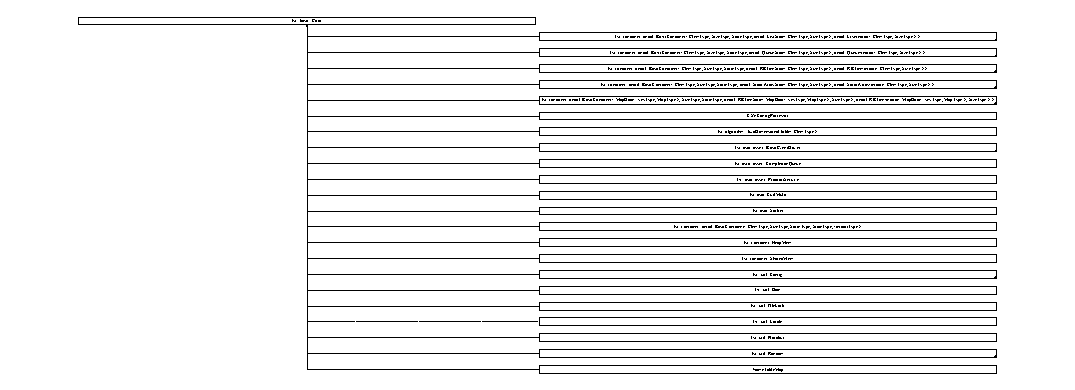
\includegraphics[height=4.7881cm]{classlsf_1_1basic_1_1Error}
\end{center}
\end{figure}
\subsection*{Public Member Functions}
\begin{DoxyCompactItemize}
\item 
\hypertarget{classlsf_1_1basic_1_1Error_aa66896c6cd0ac590bfa326d39b2a2865}{
std::string const \& {\bfseries ErrString} () const }
\label{classlsf_1_1basic_1_1Error_aa66896c6cd0ac590bfa326d39b2a2865}

\end{DoxyCompactItemize}
\subsection*{Static Public Member Functions}
\begin{DoxyCompactItemize}
\item 
\hypertarget{classlsf_1_1basic_1_1Error_aae00b39eca9e259591e3ece619bd2eca}{
static std::string {\bfseries SysErrString} ()}
\label{classlsf_1_1basic_1_1Error_aae00b39eca9e259591e3ece619bd2eca}

\end{DoxyCompactItemize}
\subsection*{Protected Member Functions}
\begin{DoxyCompactItemize}
\item 
\hypertarget{classlsf_1_1basic_1_1Error_a10932986050c12255877c402ae6f8ab7}{
{\footnotesize template$<$typename AnyType $>$ }\\AnyType {\bfseries ErrWrap} (AnyType expr) const }
\label{classlsf_1_1basic_1_1Error_a10932986050c12255877c402ae6f8ab7}

\item 
\hypertarget{classlsf_1_1basic_1_1Error_a69306bccfcf7728edfa573e4d173572f}{
{\footnotesize template$<$typename AnyType $>$ }\\AnyType {\bfseries ErrWrapPointer} (AnyType expr) const }
\label{classlsf_1_1basic_1_1Error_a69306bccfcf7728edfa573e4d173572f}

\item 
\hypertarget{classlsf_1_1basic_1_1Error_aaef55d948ef57d8ff530a0e6aa7c3c41}{
void {\bfseries SetErrString} (char const $\ast$char\_\-str) const }
\label{classlsf_1_1basic_1_1Error_aaef55d948ef57d8ff530a0e6aa7c3c41}

\item 
\hypertarget{classlsf_1_1basic_1_1Error_a7af216e3c9ebfa009d7e33f670918a41}{
void {\bfseries SetErrString} (std::string const \&str) const }
\label{classlsf_1_1basic_1_1Error_a7af216e3c9ebfa009d7e33f670918a41}

\end{DoxyCompactItemize}
\subsection*{Protected Attributes}
\begin{DoxyCompactItemize}
\item 
\hypertarget{classlsf_1_1basic_1_1Error_a97da44e3978bc4835cf44ce9ee049149}{
std::string {\bfseries \_\-err\_\-string}}
\label{classlsf_1_1basic_1_1Error_a97da44e3978bc4835cf44ce9ee049149}

\end{DoxyCompactItemize}


The documentation for this class was generated from the following file:\begin{DoxyCompactItemize}
\item 
dev/lsf/basic/error.hpp\end{DoxyCompactItemize}

\hypertarget{classlsf_1_1util_1_1FileLock}{
\section{lsf::util::FileLock Class Reference}
\label{classlsf_1_1util_1_1FileLock}\index{lsf::util::FileLock@{lsf::util::FileLock}}
}
Inheritance diagram for lsf::util::FileLock::\begin{figure}[H]
\begin{center}
\leavevmode
\includegraphics[height=2cm]{classlsf_1_1util_1_1FileLock}
\end{center}
\end{figure}
\subsection*{Public Member Functions}
\begin{DoxyCompactItemize}
\item 
\hypertarget{classlsf_1_1util_1_1FileLock_a4748fbc4b705d960f020f909c5e7a648}{
bool {\bfseries Lock} (char const $\ast$lockfile)}
\label{classlsf_1_1util_1_1FileLock_a4748fbc4b705d960f020f909c5e7a648}

\item 
\hypertarget{classlsf_1_1util_1_1FileLock_aa41e261e94e65724e58474c74ec7bf9a}{
bool {\bfseries UnLock} ()}
\label{classlsf_1_1util_1_1FileLock_aa41e261e94e65724e58474c74ec7bf9a}

\item 
\hypertarget{classlsf_1_1util_1_1FileLock_a930cbfcfe878e1e8b89b22b45d281327}{
bool {\bfseries IsLocked} ()}
\label{classlsf_1_1util_1_1FileLock_a930cbfcfe878e1e8b89b22b45d281327}

\end{DoxyCompactItemize}


The documentation for this class was generated from the following file:\begin{DoxyCompactItemize}
\item 
dev/lsf/util/file\_\-lock.hpp\end{DoxyCompactItemize}

\hypertarget{structlsf_1_1basic_1_1find__assignable_3_01T_01_4}{
\section{lsf::basic::find\_\-assignable$<$ T $>$ Struct Template Reference}
\label{structlsf_1_1basic_1_1find__assignable_3_01T_01_4}\index{lsf::basic::find\_\-assignable$<$ T $>$@{lsf::basic::find\_\-assignable$<$ T $>$}}
}
\subsubsection*{template$<$typename T$>$ struct lsf::basic::find\_\-assignable$<$ T $>$}



The documentation for this struct was generated from the following file:\begin{DoxyCompactItemize}
\item 
dev/lsf/basic/type\_\-traits.hpp\end{DoxyCompactItemize}

\hypertarget{structlsf_1_1basic_1_1find__assignable_3_01T_00_01T1_00_01Ts_8_8_8_4}{
\section{lsf::basic::find\_\-assignable$<$ T, T1, Ts...$>$ Struct Template Reference}
\label{structlsf_1_1basic_1_1find__assignable_3_01T_00_01T1_00_01Ts_8_8_8_4}\index{lsf::basic::find\_\-assignable$<$ T, T1, Ts...$>$@{lsf::basic::find\_\-assignable$<$ T, T1, Ts...$>$}}
}
\subsubsection*{template$<$typename T, typename T1, typename... Ts$>$ struct lsf::basic::find\_\-assignable$<$ T, T1, Ts...$>$}



The documentation for this struct was generated from the following file:\begin{DoxyCompactItemize}
\item 
dev/lsf/basic/type\_\-traits.hpp\end{DoxyCompactItemize}

\hypertarget{structlsf_1_1basic_1_1function__traits}{
\section{lsf::basic::function\_\-traits$<$ F $>$ Struct Template Reference}
\label{structlsf_1_1basic_1_1function__traits}\index{lsf::basic::function\_\-traits@{lsf::basic::function\_\-traits}}
}
\subsubsection*{template$<$class F$>$ struct lsf::basic::function\_\-traits$<$ F $>$}



The documentation for this struct was generated from the following file:\begin{DoxyCompactItemize}
\item 
dev/lsf/basic/type\_\-traits.hpp\end{DoxyCompactItemize}

\hypertarget{structlsf_1_1basic_1_1function__traits_3_01R_07_5_08_07Args_8_8_8_08_4}{
\section{lsf::basic::function\_\-traits$<$ R($\ast$)(Args...)$>$ Struct Template Reference}
\label{structlsf_1_1basic_1_1function__traits_3_01R_07_5_08_07Args_8_8_8_08_4}\index{lsf::basic::function\_\-traits$<$ R($\ast$)(Args...)$>$@{lsf::basic::function\_\-traits$<$ R($\ast$)(Args...)$>$}}
}
Inheritance diagram for lsf::basic::function\_\-traits$<$ R($\ast$)(Args...)$>$::\begin{figure}[H]
\begin{center}
\leavevmode
\includegraphics[height=2cm]{structlsf_1_1basic_1_1function__traits_3_01R_07_5_08_07Args_8_8_8_08_4}
\end{center}
\end{figure}
\subsubsection*{template$<$class R, class... Args$>$ struct lsf::basic::function\_\-traits$<$ R($\ast$)(Args...)$>$}



The documentation for this struct was generated from the following file:\begin{DoxyCompactItemize}
\item 
dev/lsf/basic/type\_\-traits.hpp\end{DoxyCompactItemize}

\hypertarget{structlsf_1_1basic_1_1function__traits_3_01R_07Args_8_8_8_08_4}{
\section{lsf::basic::function\_\-traits$<$ R(Args...)$>$ Struct Template Reference}
\label{structlsf_1_1basic_1_1function__traits_3_01R_07Args_8_8_8_08_4}\index{lsf::basic::function\_\-traits$<$ R(Args...)$>$@{lsf::basic::function\_\-traits$<$ R(Args...)$>$}}
}
Inheritance diagram for lsf::basic::function\_\-traits$<$ R(Args...)$>$::\begin{figure}[H]
\begin{center}
\leavevmode
\includegraphics[height=2cm]{structlsf_1_1basic_1_1function__traits_3_01R_07Args_8_8_8_08_4}
\end{center}
\end{figure}
\subsection*{Classes}
\begin{DoxyCompactItemize}
\item 
struct \hyperlink{structlsf_1_1basic_1_1function__traits_3_01R_07Args_8_8_8_08_4_1_1argument}{argument}
\end{DoxyCompactItemize}
\subsection*{Static Public Attributes}
\begin{DoxyCompactItemize}
\item 
\hypertarget{structlsf_1_1basic_1_1function__traits_3_01R_07Args_8_8_8_08_4_a3025bfe317abbbb2a4db0d4d26b2f028}{
static constexpr std::size\_\-t {\bfseries argument\_\-size} = sizeof...(Args)}
\label{structlsf_1_1basic_1_1function__traits_3_01R_07Args_8_8_8_08_4_a3025bfe317abbbb2a4db0d4d26b2f028}

\end{DoxyCompactItemize}
\subsubsection*{template$<$class R, class... Args$>$ struct lsf::basic::function\_\-traits$<$ R(Args...)$>$}



The documentation for this struct was generated from the following file:\begin{DoxyCompactItemize}
\item 
dev/lsf/basic/type\_\-traits.hpp\end{DoxyCompactItemize}

\hypertarget{structlsf_1_1basic_1_1function__traits_3_01R_07C_1_1_5_08_07Args_8_8_8_08_01const_01_01_4}{
\section{lsf::basic::function\_\-traits$<$ R(C::$\ast$)(Args...) const $>$ Struct Template Reference}
\label{structlsf_1_1basic_1_1function__traits_3_01R_07C_1_1_5_08_07Args_8_8_8_08_01const_01_01_4}\index{lsf::basic::function\_\-traits$<$ R(C::$\ast$)(Args...) const  $>$@{lsf::basic::function\_\-traits$<$ R(C::$\ast$)(Args...) const  $>$}}
}
Inheritance diagram for lsf::basic::function\_\-traits$<$ R(C::$\ast$)(Args...) const $>$::\begin{figure}[H]
\begin{center}
\leavevmode
\includegraphics[height=2cm]{structlsf_1_1basic_1_1function__traits_3_01R_07C_1_1_5_08_07Args_8_8_8_08_01const_01_01_4}
\end{center}
\end{figure}
\subsubsection*{template$<$class C, class R, class... Args$>$ struct lsf::basic::function\_\-traits$<$ R(C::$\ast$)(Args...) const  $>$}



The documentation for this struct was generated from the following file:\begin{DoxyCompactItemize}
\item 
dev/lsf/basic/type\_\-traits.hpp\end{DoxyCompactItemize}

\hypertarget{structlsf_1_1basic_1_1function__traits_3_01R_07C_1_1_5_08_07Args_8_8_8_08_4}{
\section{lsf::basic::function\_\-traits$<$ R(C::$\ast$)(Args...)$>$ Struct Template Reference}
\label{structlsf_1_1basic_1_1function__traits_3_01R_07C_1_1_5_08_07Args_8_8_8_08_4}\index{lsf::basic::function\_\-traits$<$ R(C::$\ast$)(Args...)$>$@{lsf::basic::function\_\-traits$<$ R(C::$\ast$)(Args...)$>$}}
}
Inheritance diagram for lsf::basic::function\_\-traits$<$ R(C::$\ast$)(Args...)$>$::\begin{figure}[H]
\begin{center}
\leavevmode
\includegraphics[height=2cm]{structlsf_1_1basic_1_1function__traits_3_01R_07C_1_1_5_08_07Args_8_8_8_08_4}
\end{center}
\end{figure}
\subsubsection*{template$<$class C, class R, class... Args$>$ struct lsf::basic::function\_\-traits$<$ R(C::$\ast$)(Args...)$>$}



The documentation for this struct was generated from the following file:\begin{DoxyCompactItemize}
\item 
dev/lsf/basic/type\_\-traits.hpp\end{DoxyCompactItemize}

\hypertarget{structlsf_1_1basic_1_1function__traits_3_01R_07C_1_1_5_08_4}{
\section{lsf::basic::function\_\-traits$<$ R(C::$\ast$)$>$ Struct Template Reference}
\label{structlsf_1_1basic_1_1function__traits_3_01R_07C_1_1_5_08_4}\index{lsf::basic::function\_\-traits$<$ R(C::$\ast$)$>$@{lsf::basic::function\_\-traits$<$ R(C::$\ast$)$>$}}
}
Inheritance diagram for lsf::basic::function\_\-traits$<$ R(C::$\ast$)$>$::\begin{figure}[H]
\begin{center}
\leavevmode
\includegraphics[height=2cm]{structlsf_1_1basic_1_1function__traits_3_01R_07C_1_1_5_08_4}
\end{center}
\end{figure}
\subsubsection*{template$<$class C, class R$>$ struct lsf::basic::function\_\-traits$<$ R(C::$\ast$)$>$}



The documentation for this struct was generated from the following file:\begin{DoxyCompactItemize}
\item 
dev/lsf/basic/type\_\-traits.hpp\end{DoxyCompactItemize}

\hypertarget{classGameServer}{
\section{GameServer Class Reference}
\label{classGameServer}\index{GameServer@{GameServer}}
}
Inheritance diagram for GameServer::\begin{figure}[H]
\begin{center}
\leavevmode
\includegraphics[height=3cm]{classGameServer}
\end{center}
\end{figure}
\subsection*{Public Member Functions}
\begin{DoxyCompactItemize}
\item 
\hypertarget{classGameServer_a7e20ecd0b94dc92da9e4b7564f8c0bc8}{
virtual bool {\bfseries OnRun} ()}
\label{classGameServer_a7e20ecd0b94dc92da9e4b7564f8c0bc8}

\item 
\hypertarget{classGameServer_a2174a01c41753000b241d60ac3b23ae3}{
virtual void {\bfseries OnExit} ()}
\label{classGameServer_a2174a01c41753000b241d60ac3b23ae3}

\end{DoxyCompactItemize}


The documentation for this class was generated from the following files:\begin{DoxyCompactItemize}
\item 
dev/svr/gamesvrd/game\_\-server.h\item 
dev/svr/gamesvrd/game\_\-server.cpp\end{DoxyCompactItemize}

\hypertarget{classHandlerManager}{
\section{HandlerManager Class Reference}
\label{classHandlerManager}\index{HandlerManager@{HandlerManager}}
}
Inheritance diagram for HandlerManager::\begin{figure}[H]
\begin{center}
\leavevmode
\includegraphics[height=2cm]{classHandlerManager}
\end{center}
\end{figure}
\subsection*{Static Public Member Functions}
\begin{DoxyCompactItemize}
\item 
\hypertarget{classHandlerManager_abb5d79359d60109fd740b0d5784a9cdc}{
static \hyperlink{classBasicHandler}{BasicHandler} $\ast$ {\bfseries Instance} (\hyperlink{classSession}{Session} const \&session)}
\label{classHandlerManager_abb5d79359d60109fd740b0d5784a9cdc}

\item 
\hypertarget{classHandlerManager_a9edd3b5bff2f8ba85e881c9afdb2d1e6}{
static \hyperlink{classBasicHandler}{BasicHandler} $\ast$ {\bfseries Instance} (msg::CS const \&message)}
\label{classHandlerManager_a9edd3b5bff2f8ba85e881c9afdb2d1e6}

\item 
\hypertarget{classHandlerManager_ab28fbca3c32dd7c2b842e4ee72addf7d}{
static \hyperlink{classBasicHandler}{BasicHandler} $\ast$ {\bfseries Instance} (msg::SS const \&message)}
\label{classHandlerManager_ab28fbca3c32dd7c2b842e4ee72addf7d}

\item 
\hypertarget{classHandlerManager_ab611079886d53d01c7122850bf403f20}{
static bool {\bfseries IsRequest} (msg::ENSSType msg\_\-type)}
\label{classHandlerManager_ab611079886d53d01c7122850bf403f20}

\item 
\hypertarget{classHandlerManager_af30ab96bb15ad16cd90e008c133309e8}{
{\footnotesize template$<$typename HandlerType $>$ }\\static void {\bfseries AddCSHandler} (msg::ENCSType req\_\-msg\_\-type, msg::ENCSType rsp\_\-msg\_\-type=msg::CS\_\-TYPE\_\-NONE)}
\label{classHandlerManager_af30ab96bb15ad16cd90e008c133309e8}

\item 
\hypertarget{classHandlerManager_a8761357449137f777cb09cef21032dd5}{
{\footnotesize template$<$typename HandlerType $>$ }\\static void {\bfseries AddSSHandler} (msg::ENSSType req\_\-msg\_\-type, msg::ENSSType rsp\_\-msg\_\-type=msg::SS\_\-TYPE\_\-NONE)}
\label{classHandlerManager_a8761357449137f777cb09cef21032dd5}

\end{DoxyCompactItemize}


The documentation for this class was generated from the following files:\begin{DoxyCompactItemize}
\item 
dev/svr/common/handler\_\-manager.h\item 
dev/svr/common/handler\_\-manager.cpp\end{DoxyCompactItemize}

\hypertarget{structstd_1_1hash_3_01lsf_1_1asio_1_1Curl_01_4}{
\section{std::hash$<$ lsf::asio::Curl $>$ Struct Template Reference}
\label{structstd_1_1hash_3_01lsf_1_1asio_1_1Curl_01_4}\index{std::hash$<$ lsf::asio::Curl $>$@{std::hash$<$ lsf::asio::Curl $>$}}
}
\subsection*{Public Member Functions}
\begin{DoxyCompactItemize}
\item 
\hypertarget{structstd_1_1hash_3_01lsf_1_1asio_1_1Curl_01_4_a41d7790ec16532992fb51b9a2b62be21}{
size\_\-t {\bfseries operator()} (\hyperlink{classlsf_1_1asio_1_1Curl}{lsf::asio::Curl} const \&curl) const }
\label{structstd_1_1hash_3_01lsf_1_1asio_1_1Curl_01_4_a41d7790ec16532992fb51b9a2b62be21}

\end{DoxyCompactItemize}
\subsubsection*{template$<$$>$ struct std::hash$<$ lsf::asio::Curl $>$}



The documentation for this struct was generated from the following file:\begin{DoxyCompactItemize}
\item 
dev/lsf/asio/curl.hpp\end{DoxyCompactItemize}

\hypertarget{structstd_1_1hash_3_01lsf_1_1asio_1_1Socket_01_4}{
\section{std::hash$<$ lsf::asio::Socket $>$ Struct Template Reference}
\label{structstd_1_1hash_3_01lsf_1_1asio_1_1Socket_01_4}\index{std::hash$<$ lsf::asio::Socket $>$@{std::hash$<$ lsf::asio::Socket $>$}}
}
\subsection*{Public Member Functions}
\begin{DoxyCompactItemize}
\item 
\hypertarget{structstd_1_1hash_3_01lsf_1_1asio_1_1Socket_01_4_a70c3d8ee09ed782151442dcc7487bcc8}{
size\_\-t {\bfseries operator()} (\hyperlink{classlsf_1_1asio_1_1Socket}{lsf::asio::Socket} const \&sock) const }
\label{structstd_1_1hash_3_01lsf_1_1asio_1_1Socket_01_4_a70c3d8ee09ed782151442dcc7487bcc8}

\end{DoxyCompactItemize}
\subsubsection*{template$<$$>$ struct std::hash$<$ lsf::asio::Socket $>$}



The documentation for this struct was generated from the following file:\begin{DoxyCompactItemize}
\item 
dev/lsf/asio/socket.hpp\end{DoxyCompactItemize}

\hypertarget{classmsg_1_1Header}{
\section{msg::Header Class Reference}
\label{classmsg_1_1Header}\index{msg::Header@{msg::Header}}
}
\subsection*{Public Member Functions}
\begin{DoxyCompactItemize}
\item 
\hypertarget{classmsg_1_1Header_a963a8444c026ef4e91e4f27a909315ea}{
void {\bfseries ntoh} ()}
\label{classmsg_1_1Header_a963a8444c026ef4e91e4f27a909315ea}

\item 
\hypertarget{classmsg_1_1Header_a5311d5957a4d6cd07b48fd53f5975dc6}{
void {\bfseries hton} ()}
\label{classmsg_1_1Header_a5311d5957a4d6cd07b48fd53f5975dc6}

\end{DoxyCompactItemize}
\subsection*{Public Attributes}
\begin{DoxyCompactItemize}
\item 
\hypertarget{classmsg_1_1Header_a59e56aecbff914a3d65f8ea49885dde8}{
uint8\_\-t {\bfseries magic} \mbox{[}2\mbox{]}}
\label{classmsg_1_1Header_a59e56aecbff914a3d65f8ea49885dde8}

\item 
\hypertarget{classmsg_1_1Header_a4ce6ee4b8d3940a87b86a22c7c4a8537}{
uint32\_\-t {\bfseries length}}
\label{classmsg_1_1Header_a4ce6ee4b8d3940a87b86a22c7c4a8537}

\end{DoxyCompactItemize}


The documentation for this class was generated from the following file:\begin{DoxyCompactItemize}
\item 
dev/svr/common/common\_\-proto.h\end{DoxyCompactItemize}

\hypertarget{classlsf_1_1container_1_1HeapMem}{
\section{lsf::container::HeapMem Class Reference}
\label{classlsf_1_1container_1_1HeapMem}\index{lsf::container::HeapMem@{lsf::container::HeapMem}}
}
Inheritance diagram for lsf::container::HeapMem::\begin{figure}[H]
\begin{center}
\leavevmode
\includegraphics[height=2cm]{classlsf_1_1container_1_1HeapMem}
\end{center}
\end{figure}
\subsection*{Public Member Functions}
\begin{DoxyCompactItemize}
\item 
\hypertarget{classlsf_1_1container_1_1HeapMem_a6c27c0e241eb309cbb3dc1178a8f8213}{
{\bfseries HeapMem} (size\_\-t byte\_\-size)}
\label{classlsf_1_1container_1_1HeapMem_a6c27c0e241eb309cbb3dc1178a8f8213}

\item 
\hypertarget{classlsf_1_1container_1_1HeapMem_a67f599680ce40b7329f8fa5690a26c90}{
void {\bfseries Malloc} (size\_\-t byte\_\-size)}
\label{classlsf_1_1container_1_1HeapMem_a67f599680ce40b7329f8fa5690a26c90}

\item 
\hypertarget{classlsf_1_1container_1_1HeapMem_a49be32275cc2b6be267a95480a6d75c5}{
void $\ast$ {\bfseries GetPtr} () const }
\label{classlsf_1_1container_1_1HeapMem_a49be32275cc2b6be267a95480a6d75c5}

\item 
\hypertarget{classlsf_1_1container_1_1HeapMem_a02a93262e5348e2b91dd912912680f51}{
size\_\-t {\bfseries GetSize} () const }
\label{classlsf_1_1container_1_1HeapMem_a02a93262e5348e2b91dd912912680f51}

\item 
\hypertarget{classlsf_1_1container_1_1HeapMem_a8364cacd04f3973b019ab44bb009cb41}{
size\_\-t {\bfseries GetUseCount} () const }
\label{classlsf_1_1container_1_1HeapMem_a8364cacd04f3973b019ab44bb009cb41}

\end{DoxyCompactItemize}


The documentation for this class was generated from the following file:\begin{DoxyCompactItemize}
\item 
dev/lsf/container/heap\_\-mem.hpp\end{DoxyCompactItemize}

\hypertarget{classHttpServer}{
\section{HttpServer Class Reference}
\label{classHttpServer}\index{HttpServer@{HttpServer}}
}
Inheritance diagram for HttpServer::\begin{figure}[H]
\begin{center}
\leavevmode
\includegraphics[height=3cm]{classHttpServer}
\end{center}
\end{figure}
\subsection*{Public Member Functions}
\begin{DoxyCompactItemize}
\item 
\hypertarget{classHttpServer_a368013113d8d8330b00c714096fc31dd}{
virtual bool {\bfseries OnRun} ()}
\label{classHttpServer_a368013113d8d8330b00c714096fc31dd}

\item 
\hypertarget{classHttpServer_ac8360438ce6e6b4eb28869c0dead8493}{
virtual void {\bfseries OnExit} ()}
\label{classHttpServer_ac8360438ce6e6b4eb28869c0dead8493}

\end{DoxyCompactItemize}


The documentation for this class was generated from the following files:\begin{DoxyCompactItemize}
\item 
dev/svr/httpsvrd/http\_\-server.h\item 
dev/svr/httpsvrd/http\_\-server.cpp\end{DoxyCompactItemize}

\hypertarget{classHttpService}{
\section{HttpService Class Reference}
\label{classHttpService}\index{HttpService@{HttpService}}
}
Inheritance diagram for HttpService::\begin{figure}[H]
\begin{center}
\leavevmode
\includegraphics[height=2cm]{classHttpService}
\end{center}
\end{figure}
\subsection*{Public Member Functions}
\begin{DoxyCompactItemize}
\item 
\hypertarget{classHttpService_a296e11a4bb783c4c3b76550b598f9344}{
bool {\bfseries Init} ()}
\label{classHttpService_a296e11a4bb783c4c3b76550b598f9344}

\item 
\hypertarget{classHttpService_a9fd7dbfe5ccade21bf3a0403ddf14d8a}{
void {\bfseries Exit} ()}
\label{classHttpService_a9fd7dbfe5ccade21bf3a0403ddf14d8a}

\end{DoxyCompactItemize}
\subsection*{Protected Member Functions}
\begin{DoxyCompactItemize}
\item 
\hypertarget{classHttpService_a145a834bce30b1a90c7d64dd0486142c}{
void {\bfseries MatchSvrGmOperation} (std::string query, std::string body)}
\label{classHttpService_a145a834bce30b1a90c7d64dd0486142c}

\item 
\hypertarget{classHttpService_a816ab28ee9302f74c8ee9ee1ed72d3c0}{
void {\bfseries GeneralSvrGmOperation} (std::string query, std::string body)}
\label{classHttpService_a816ab28ee9302f74c8ee9ee1ed72d3c0}

\item 
\hypertarget{classHttpService_a925991674186ae4dca2b788363d8bad6}{
bool {\bfseries ParseJson} (std::string uri, std::string const content)}
\label{classHttpService_a925991674186ae4dca2b788363d8bad6}

\item 
\hypertarget{classHttpService_a006e7756b3098fd7b3162058ad32e4d0}{
bool {\bfseries QueryStr2Message} (std::string query, ProtobufMsg \&message)}
\label{classHttpService_a006e7756b3098fd7b3162058ad32e4d0}

\end{DoxyCompactItemize}
\subsection*{Static Protected Attributes}
\begin{DoxyCompactItemize}
\item 
\hypertarget{classHttpService_aec9ec5c4f2eb9a7ecba8207d47f2509d}{
static const size\_\-t {\bfseries DEF\_\-CHECK\_\-INTERVAL} = 10}
\label{classHttpService_aec9ec5c4f2eb9a7ecba8207d47f2509d}

\item 
\hypertarget{classHttpService_addfbf7a63fdb80db25b5287d8a8a8179}{
static const size\_\-t {\bfseries DEF\_\-LOOP\_\-TIME} = 0}
\label{classHttpService_addfbf7a63fdb80db25b5287d8a8a8179}

\end{DoxyCompactItemize}


The documentation for this class was generated from the following files:\begin{DoxyCompactItemize}
\item 
dev/svr/httpsvrd/http\_\-service.h\item 
dev/svr/httpsvrd/http\_\-service.cpp\end{DoxyCompactItemize}

\hypertarget{structlsf_1_1basic_1_1index_3_01T_01_4}{
\section{lsf::basic::index$<$ T $>$ Struct Template Reference}
\label{structlsf_1_1basic_1_1index_3_01T_01_4}\index{lsf::basic::index$<$ T $>$@{lsf::basic::index$<$ T $>$}}
}
Inheritance diagram for lsf::basic::index$<$ T $>$::\begin{figure}[H]
\begin{center}
\leavevmode
\includegraphics[height=2cm]{structlsf_1_1basic_1_1index_3_01T_01_4}
\end{center}
\end{figure}
\subsubsection*{template$<$typename T$>$ struct lsf::basic::index$<$ T $>$}



The documentation for this struct was generated from the following file:\begin{DoxyCompactItemize}
\item 
dev/lsf/basic/type\_\-traits.hpp\end{DoxyCompactItemize}

\hypertarget{structlsf_1_1basic_1_1index_3_01T_00_01First_00_01Ts_8_8_8_4}{
\section{lsf::basic::index$<$ T, First, Ts...$>$ Struct Template Reference}
\label{structlsf_1_1basic_1_1index_3_01T_00_01First_00_01Ts_8_8_8_4}\index{lsf::basic::index$<$ T, First, Ts...$>$@{lsf::basic::index$<$ T, First, Ts...$>$}}
}
\subsubsection*{template$<$typename T, typename First, typename... Ts$>$ struct lsf::basic::index$<$ T, First, Ts...$>$}



The documentation for this struct was generated from the following file:\begin{DoxyCompactItemize}
\item 
dev/lsf/basic/type\_\-traits.hpp\end{DoxyCompactItemize}

\hypertarget{structlsf_1_1basic_1_1index_3_01T_00_01T_00_01Ts_8_8_8_4}{
\section{lsf::basic::index$<$ T, T, Ts...$>$ Struct Template Reference}
\label{structlsf_1_1basic_1_1index_3_01T_00_01T_00_01Ts_8_8_8_4}\index{lsf::basic::index$<$ T, T, Ts...$>$@{lsf::basic::index$<$ T, T, Ts...$>$}}
}
Inheritance diagram for lsf::basic::index$<$ T, T, Ts...$>$::\begin{figure}[H]
\begin{center}
\leavevmode
\includegraphics[height=2cm]{structlsf_1_1basic_1_1index_3_01T_00_01T_00_01Ts_8_8_8_4}
\end{center}
\end{figure}
\subsubsection*{template$<$typename T, typename... Ts$>$ struct lsf::basic::index$<$ T, T, Ts...$>$}



The documentation for this struct was generated from the following file:\begin{DoxyCompactItemize}
\item 
dev/lsf/basic/type\_\-traits.hpp\end{DoxyCompactItemize}

\hypertarget{structlsf_1_1basic_1_1index__type}{
\section{lsf::basic::index\_\-type$<$ N, Ts $>$ Struct Template Reference}
\label{structlsf_1_1basic_1_1index__type}\index{lsf::basic::index\_\-type@{lsf::basic::index\_\-type}}
}
\subsection*{Public Member Functions}
\begin{DoxyCompactItemize}
\item 
\hypertarget{structlsf_1_1basic_1_1index__type_aabe14ee1791f8fc3c5212eacdeffa378}{
{\bfseries static\_\-assert} (N$<$ sizeof...(Ts), LSF\_\-DEBUG\_\-INFO)}
\label{structlsf_1_1basic_1_1index__type_aabe14ee1791f8fc3c5212eacdeffa378}

\end{DoxyCompactItemize}
\subsubsection*{template$<$int N, typename... Ts$>$ struct lsf::basic::index\_\-type$<$ N, Ts $>$}



The documentation for this struct was generated from the following file:\begin{DoxyCompactItemize}
\item 
dev/lsf/basic/type\_\-traits.hpp\end{DoxyCompactItemize}

\hypertarget{classInsertDataHandler}{
\section{InsertDataHandler Class Reference}
\label{classInsertDataHandler}\index{InsertDataHandler@{InsertDataHandler}}
}
Inheritance diagram for InsertDataHandler::\begin{figure}[H]
\begin{center}
\leavevmode
\includegraphics[height=2cm]{classInsertDataHandler}
\end{center}
\end{figure}
\subsection*{Public Member Functions}
\begin{DoxyCompactItemize}
\item 
\hypertarget{classInsertDataHandler_a5a8ec18efb9e5e7f6d967820bf5e8f05}{
virtual data::ENSessionState {\bfseries OnServerRequest} (\hyperlink{classSession}{Session} \&session)}
\label{classInsertDataHandler_a5a8ec18efb9e5e7f6d967820bf5e8f05}

\end{DoxyCompactItemize}


The documentation for this class was generated from the following files:\begin{DoxyCompactItemize}
\item 
dev/svr/datasvrd/handler\_\-common.h\item 
dev/svr/datasvrd/handler\_\-common.cpp\end{DoxyCompactItemize}

\hypertarget{structlsf_1_1basic_1_1integer__max_3_01Arg_01_4}{
\section{lsf::basic::integer\_\-max$<$ Arg $>$ Struct Template Reference}
\label{structlsf_1_1basic_1_1integer__max_3_01Arg_01_4}\index{lsf::basic::integer\_\-max$<$ Arg $>$@{lsf::basic::integer\_\-max$<$ Arg $>$}}
}
\subsubsection*{template$<$size\_\-t Arg$>$ struct lsf::basic::integer\_\-max$<$ Arg $>$}



The documentation for this struct was generated from the following file:\begin{DoxyCompactItemize}
\item 
dev/lsf/basic/type\_\-traits.hpp\end{DoxyCompactItemize}

\hypertarget{structlsf_1_1basic_1_1integer__max_3_01arg1_00_01arg2_00_01Rest_8_8_8_4}{
\section{lsf::basic::integer\_\-max$<$ arg1, arg2, Rest...$>$ Struct Template Reference}
\label{structlsf_1_1basic_1_1integer__max_3_01arg1_00_01arg2_00_01Rest_8_8_8_4}\index{lsf::basic::integer\_\-max$<$ arg1, arg2, Rest...$>$@{lsf::basic::integer\_\-max$<$ arg1, arg2, Rest...$>$}}
}
\subsubsection*{template$<$size\_\-t arg1, size\_\-t arg2, size\_\-t... Rest$>$ struct lsf::basic::integer\_\-max$<$ arg1, arg2, Rest...$>$}



The documentation for this struct was generated from the following file:\begin{DoxyCompactItemize}
\item 
dev/lsf/basic/type\_\-traits.hpp\end{DoxyCompactItemize}

\hypertarget{classlsf_1_1asio_1_1IOService}{
\section{lsf::asio::IOService Class Reference}
\label{classlsf_1_1asio_1_1IOService}\index{lsf::asio::IOService@{lsf::asio::IOService}}
}
\subsection*{Classes}
\begin{DoxyCompactItemize}
\item 
class \hyperlink{classlsf_1_1asio_1_1IOService_1_1IOServiceContent}{IOServiceContent}
\end{DoxyCompactItemize}
\subsection*{Static Public Member Functions}
\begin{DoxyCompactItemize}
\item 
\hypertarget{classlsf_1_1asio_1_1IOService_a12e246738882eb0b19d5826da7c7e197}{
static ProactorSerivce $\ast$ {\bfseries Instance} ()}
\label{classlsf_1_1asio_1_1IOService_a12e246738882eb0b19d5826da7c7e197}

\item 
\hypertarget{classlsf_1_1asio_1_1IOService_a3243c6a8350cbfe62938eef04ebcda30}{
static ProactorSerivce \& {\bfseries Reference} ()}
\label{classlsf_1_1asio_1_1IOService_a3243c6a8350cbfe62938eef04ebcda30}

\item 
\hypertarget{classlsf_1_1asio_1_1IOService_a6d26e8b63283c1613b355bdff61cb58e}{
static void {\bfseries UseEpoll} ()}
\label{classlsf_1_1asio_1_1IOService_a6d26e8b63283c1613b355bdff61cb58e}

\item 
\hypertarget{classlsf_1_1asio_1_1IOService_a4e07f4ba20be9c1454efaa9b70b990ab}{
static void {\bfseries UsePoll} ()}
\label{classlsf_1_1asio_1_1IOService_a4e07f4ba20be9c1454efaa9b70b990ab}

\end{DoxyCompactItemize}
\subsection*{Static Public Attributes}
\begin{DoxyCompactItemize}
\item 
\hypertarget{classlsf_1_1asio_1_1IOService_afb05c1b261e1718e3567989ba995ddee}{
static const int {\bfseries FLAG\_\-READ} = async::BasicEventDriver::FLAG\_\-READ}
\label{classlsf_1_1asio_1_1IOService_afb05c1b261e1718e3567989ba995ddee}

\item 
\hypertarget{classlsf_1_1asio_1_1IOService_a3f4c0b9420386fe3a2c55b4873f0d783}{
static const int {\bfseries FLAG\_\-WRITE} = async::BasicEventDriver::FLAG\_\-WRITE}
\label{classlsf_1_1asio_1_1IOService_a3f4c0b9420386fe3a2c55b4873f0d783}

\item 
\hypertarget{classlsf_1_1asio_1_1IOService_af1e67e6626eb87a669db15538e9a8e9f}{
static const int {\bfseries FLAG\_\-ERR} = async::BasicEventDriver::FLAG\_\-ERR}
\label{classlsf_1_1asio_1_1IOService_af1e67e6626eb87a669db15538e9a8e9f}

\end{DoxyCompactItemize}
\subsection*{Protected Member Functions}
\begin{DoxyCompactItemize}
\item 
\hypertarget{classlsf_1_1asio_1_1IOService_a4733d5afe2c1233cf2ed0edeaa100abd}{
{\bfseries IOService} (\hyperlink{classlsf_1_1asio_1_1IOService}{IOService} const \&)}
\label{classlsf_1_1asio_1_1IOService_a4733d5afe2c1233cf2ed0edeaa100abd}

\item 
\hypertarget{classlsf_1_1asio_1_1IOService_a12ed35d6b137443d22ca1f7f65416b6e}{
\hyperlink{classlsf_1_1asio_1_1IOService}{IOService} \& {\bfseries operator=} (\hyperlink{classlsf_1_1asio_1_1IOService}{IOService} const \&)}
\label{classlsf_1_1asio_1_1IOService_a12ed35d6b137443d22ca1f7f65416b6e}

\end{DoxyCompactItemize}


The documentation for this class was generated from the following file:\begin{DoxyCompactItemize}
\item 
dev/lsf/asio/async.hpp\end{DoxyCompactItemize}

\hypertarget{classlsf_1_1asio_1_1IOService_1_1IOServiceContent}{
\section{lsf::asio::IOService::IOServiceContent Class Reference}
\label{classlsf_1_1asio_1_1IOService_1_1IOServiceContent}\index{lsf::asio::IOService::IOServiceContent@{lsf::asio::IOService::IOServiceContent}}
}
Inheritance diagram for lsf::asio::IOService::IOServiceContent::\begin{figure}[H]
\begin{center}
\leavevmode
\includegraphics[height=2cm]{classlsf_1_1asio_1_1IOService_1_1IOServiceContent}
\end{center}
\end{figure}
\subsection*{Public Attributes}
\begin{DoxyCompactItemize}
\item 
\hypertarget{classlsf_1_1asio_1_1IOService_1_1IOServiceContent_ad8e87d11d1fe2b0eac7d44bfac78fc4e}{
bool {\bfseries use\_\-epoll} = false}
\label{classlsf_1_1asio_1_1IOService_1_1IOServiceContent_ad8e87d11d1fe2b0eac7d44bfac78fc4e}

\item 
\hypertarget{classlsf_1_1asio_1_1IOService_1_1IOServiceContent_a695ecbcc6620529ab850254c9793a93c}{
ProactorSerivce $\ast$ {\bfseries epoll\_\-service} = nullptr}
\label{classlsf_1_1asio_1_1IOService_1_1IOServiceContent_a695ecbcc6620529ab850254c9793a93c}

\item 
\hypertarget{classlsf_1_1asio_1_1IOService_1_1IOServiceContent_a303ab2cecbc272778560d1a3237e02d6}{
ProactorSerivce $\ast$ {\bfseries poll\_\-service} = nullptr}
\label{classlsf_1_1asio_1_1IOService_1_1IOServiceContent_a303ab2cecbc272778560d1a3237e02d6}

\end{DoxyCompactItemize}


The documentation for this class was generated from the following file:\begin{DoxyCompactItemize}
\item 
dev/lsf/asio/async.hpp\end{DoxyCompactItemize}

\hypertarget{structlsf_1_1basic_1_1is__assignable}{
\section{lsf::basic::is\_\-assignable$<$ T1, T2 $>$ Struct Template Reference}
\label{structlsf_1_1basic_1_1is__assignable}\index{lsf::basic::is\_\-assignable@{lsf::basic::is\_\-assignable}}
}
\subsubsection*{template$<$typename T1, typename T2$>$ struct lsf::basic::is\_\-assignable$<$ T1, T2 $>$}



The documentation for this struct was generated from the following file:\begin{DoxyCompactItemize}
\item 
dev/lsf/basic/type\_\-traits.hpp\end{DoxyCompactItemize}

\hypertarget{structlsf_1_1basic_1_1is__assignable_3_01double_00_01float_01_4}{
\section{lsf::basic::is\_\-assignable$<$ double, float $>$ Struct Template Reference}
\label{structlsf_1_1basic_1_1is__assignable_3_01double_00_01float_01_4}\index{lsf::basic::is\_\-assignable$<$ double, float $>$@{lsf::basic::is\_\-assignable$<$ double, float $>$}}
}
\subsubsection*{template$<$$>$ struct lsf::basic::is\_\-assignable$<$ double, float $>$}



The documentation for this struct was generated from the following file:\begin{DoxyCompactItemize}
\item 
dev/lsf/basic/type\_\-traits.hpp\end{DoxyCompactItemize}

\hypertarget{structlsf_1_1basic_1_1is__assignable_3_01float_00_01double_01_4}{
\section{lsf::basic::is\_\-assignable$<$ float, double $>$ Struct Template Reference}
\label{structlsf_1_1basic_1_1is__assignable_3_01float_00_01double_01_4}\index{lsf::basic::is\_\-assignable$<$ float, double $>$@{lsf::basic::is\_\-assignable$<$ float, double $>$}}
}
\subsubsection*{template$<$$>$ struct lsf::basic::is\_\-assignable$<$ float, double $>$}



The documentation for this struct was generated from the following file:\begin{DoxyCompactItemize}
\item 
dev/lsf/basic/type\_\-traits.hpp\end{DoxyCompactItemize}

\hypertarget{structlsf_1_1basic_1_1is__assignable_3_01T_01const_01_5_00_01T_01_5_01_4}{
\section{lsf::basic::is\_\-assignable$<$ T const $\ast$, T $\ast$ $>$ Struct Template Reference}
\label{structlsf_1_1basic_1_1is__assignable_3_01T_01const_01_5_00_01T_01_5_01_4}\index{lsf::basic::is\_\-assignable$<$ T const $\ast$, T $\ast$ $>$@{lsf::basic::is\_\-assignable$<$ T const $\ast$, T $\ast$ $>$}}
}
\subsubsection*{template$<$typename T$>$ struct lsf::basic::is\_\-assignable$<$ T const $\ast$, T $\ast$ $>$}



The documentation for this struct was generated from the following file:\begin{DoxyCompactItemize}
\item 
dev/lsf/basic/type\_\-traits.hpp\end{DoxyCompactItemize}

\hypertarget{classLevelDBManager}{
\section{LevelDBManager Class Reference}
\label{classLevelDBManager}\index{LevelDBManager@{LevelDBManager}}
}
Inheritance diagram for LevelDBManager::\begin{figure}[H]
\begin{center}
\leavevmode
\includegraphics[height=2cm]{classLevelDBManager}
\end{center}
\end{figure}
\subsection*{Public Member Functions}
\begin{DoxyCompactItemize}
\item 
\hypertarget{classLevelDBManager_a9bb2eb976391a3a9dbef61c04d328a7c}{
bool {\bfseries Init} (size\_\-t leveldb\_\-cache, std::string const \&leveldb\_\-path)}
\label{classLevelDBManager_a9bb2eb976391a3a9dbef61c04d328a7c}

\item 
\hypertarget{classLevelDBManager_a59807591eb91c7438e39d63851ce1868}{
bool {\bfseries Has} (std::string const \&key)}
\label{classLevelDBManager_a59807591eb91c7438e39d63851ce1868}

\item 
\hypertarget{classLevelDBManager_aa28f74df620826d4692e91d8b04bb2ca}{
bool {\bfseries Query} (std::string const \&key, google::protobuf::Message \&message)}
\label{classLevelDBManager_aa28f74df620826d4692e91d8b04bb2ca}

\item 
\hypertarget{classLevelDBManager_a31004736e82748b2bff292b150dbfa1a}{
bool {\bfseries Query} (std::string const \&key, std::string \&content)}
\label{classLevelDBManager_a31004736e82748b2bff292b150dbfa1a}

\item 
\hypertarget{classLevelDBManager_a9522ef00c5e43ca71f4b24f9abfdca24}{
bool {\bfseries Update} (std::string const \&key, google::protobuf::Message const \&message)}
\label{classLevelDBManager_a9522ef00c5e43ca71f4b24f9abfdca24}

\item 
\hypertarget{classLevelDBManager_aa7fdee6fea29ffc7810254c2251d845e}{
bool {\bfseries Update} (std::string const \&key, std::string const \&content)}
\label{classLevelDBManager_aa7fdee6fea29ffc7810254c2251d845e}

\item 
\hypertarget{classLevelDBManager_a865672541d3f4a9a9a9ad350ea19d390}{
bool {\bfseries Delete} (std::string const \&key)}
\label{classLevelDBManager_a865672541d3f4a9a9a9ad350ea19d390}

\item 
\hypertarget{classLevelDBManager_a50ad4e7d39bd513d9d0e51230e8d5f2b}{
bool {\bfseries BatchUpdate} (std::vector$<$ \hyperlink{structDBBatchInfo}{DBBatchInfo} $>$ const \&batch\_\-ops)}
\label{classLevelDBManager_a50ad4e7d39bd513d9d0e51230e8d5f2b}

\end{DoxyCompactItemize}


The documentation for this class was generated from the following files:\begin{DoxyCompactItemize}
\item 
dev/svr/datasvrd/leveldb\_\-manager.h\item 
dev/svr/datasvrd/leveldb\_\-manager.cpp\end{DoxyCompactItemize}

\hypertarget{classlsf_1_1container_1_1List}{
\section{lsf::container::List$<$ ElemType, StoreType, SizeType $>$ Class Template Reference}
\label{classlsf_1_1container_1_1List}\index{lsf::container::List@{lsf::container::List}}
}
Inheritance diagram for lsf::container::List$<$ ElemType, StoreType, SizeType $>$::\begin{figure}[H]
\begin{center}
\leavevmode
\includegraphics[height=0.930233cm]{classlsf_1_1container_1_1List}
\end{center}
\end{figure}
\subsection*{Public Member Functions}
\begin{DoxyCompactItemize}
\item 
\hypertarget{classlsf_1_1container_1_1List_a53bf2732ee98a81538ded7bb0d06b3ad}{
bool {\bfseries PushBack} (value\_\-type const \&val)}
\label{classlsf_1_1container_1_1List_a53bf2732ee98a81538ded7bb0d06b3ad}

\item 
\hypertarget{classlsf_1_1container_1_1List_a34e085a9059d7b09552929952036efe6}{
bool {\bfseries PushFront} (value\_\-type const \&val)}
\label{classlsf_1_1container_1_1List_a34e085a9059d7b09552929952036efe6}

\item 
\hypertarget{classlsf_1_1container_1_1List_a990f0ca85ebf89299df90966b8f39292}{
bool {\bfseries PopFront} ()}
\label{classlsf_1_1container_1_1List_a990f0ca85ebf89299df90966b8f39292}

\item 
\hypertarget{classlsf_1_1container_1_1List_a2d85df79eb6ee0f7459dd64822d346e9}{
bool {\bfseries PopBack} ()}
\label{classlsf_1_1container_1_1List_a2d85df79eb6ee0f7459dd64822d346e9}

\item 
\hypertarget{classlsf_1_1container_1_1List_a5e2ef05129487b53eb282e7090fd7383}{
bool {\bfseries Insert} (iterator iter, value\_\-type const \&val)}
\label{classlsf_1_1container_1_1List_a5e2ef05129487b53eb282e7090fd7383}

\item 
\hypertarget{classlsf_1_1container_1_1List_ad8ee8e958e0dd3d17ef915c5b10e4f39}{
bool {\bfseries Erase} (iterator iter)}
\label{classlsf_1_1container_1_1List_ad8ee8e958e0dd3d17ef915c5b10e4f39}

\item 
\hypertarget{classlsf_1_1container_1_1List_a39e3d412da56ec7536941e16f2371942}{
bool {\bfseries Erase} (iterator iter\_\-st, iterator iter\_\-ed)}
\label{classlsf_1_1container_1_1List_a39e3d412da56ec7536941e16f2371942}

\item 
\hypertarget{classlsf_1_1container_1_1List_a4638a80895a4cc7f5f26609c1301547a}{
iterator {\bfseries Find} (value\_\-type const \&val)}
\label{classlsf_1_1container_1_1List_a4638a80895a4cc7f5f26609c1301547a}

\item 
\hypertarget{classlsf_1_1container_1_1List_ae2a63f292345bc54c71dba51ef9bcbf8}{
iterator {\bfseries GetFront} ()}
\label{classlsf_1_1container_1_1List_ae2a63f292345bc54c71dba51ef9bcbf8}

\item 
\hypertarget{classlsf_1_1container_1_1List_aa58c0f86a0a46e3b3878ac990de0b2c5}{
iterator {\bfseries GetBack} ()}
\label{classlsf_1_1container_1_1List_aa58c0f86a0a46e3b3878ac990de0b2c5}

\item 
\hypertarget{classlsf_1_1container_1_1List_a78dea9b87564d39ebe811239822d537a}{
iterator {\bfseries begin} ()}
\label{classlsf_1_1container_1_1List_a78dea9b87564d39ebe811239822d537a}

\item 
\hypertarget{classlsf_1_1container_1_1List_a16a74e517082b29bec47fc26d7186498}{
iterator {\bfseries end} ()}
\label{classlsf_1_1container_1_1List_a16a74e517082b29bec47fc26d7186498}

\item 
\hypertarget{classlsf_1_1container_1_1List_ae1278e2a8ea48485cdbb8907ba25265a}{
reverse\_\-iterator {\bfseries rbegin} ()}
\label{classlsf_1_1container_1_1List_ae1278e2a8ea48485cdbb8907ba25265a}

\item 
\hypertarget{classlsf_1_1container_1_1List_acef3625dc1aa09c4c941710410d7f592}{
reverse\_\-iterator {\bfseries rend} ()}
\label{classlsf_1_1container_1_1List_acef3625dc1aa09c4c941710410d7f592}

\end{DoxyCompactItemize}
\subsubsection*{template$<$typename ElemType = lsf::basic::EmptyType, typename StoreType = SharedMem, typename SizeType = size\_\-t$>$ class lsf::container::List$<$ ElemType, StoreType, SizeType $>$}



The documentation for this class was generated from the following file:\begin{DoxyCompactItemize}
\item 
dev/lsf/container/list.hpp\end{DoxyCompactItemize}

\hypertarget{classlsf_1_1container_1_1detail_1_1ListIterator}{
\section{lsf::container::detail::ListIterator$<$ ElemType, SizeType $>$ Class Template Reference}
\label{classlsf_1_1container_1_1detail_1_1ListIterator}\index{lsf::container::detail::ListIterator@{lsf::container::detail::ListIterator}}
}
\subsection*{Public Member Functions}
\begin{DoxyCompactItemize}
\item 
\hypertarget{classlsf_1_1container_1_1detail_1_1ListIterator_a737b012d4138d227dcbfb31c9a721ba2}{
{\bfseries ListIterator} (state\_\-type $\ast$ptr\_\-state=nullptr, size\_\-type pos=0)}
\label{classlsf_1_1container_1_1detail_1_1ListIterator_a737b012d4138d227dcbfb31c9a721ba2}

\item 
\hypertarget{classlsf_1_1container_1_1detail_1_1ListIterator_a23c39ffbc9244d26b856a64e299db1af}{
\hyperlink{classlsf_1_1container_1_1detail_1_1ListIterator}{ListIterator} {\bfseries operator+} (difference\_\-type diff) const }
\label{classlsf_1_1container_1_1detail_1_1ListIterator_a23c39ffbc9244d26b856a64e299db1af}

\item 
\hypertarget{classlsf_1_1container_1_1detail_1_1ListIterator_a76f943d712b5751198b316ec5798a4d7}{
\hyperlink{classlsf_1_1container_1_1detail_1_1ListIterator}{ListIterator} {\bfseries operator-\/} (difference\_\-type diff) const }
\label{classlsf_1_1container_1_1detail_1_1ListIterator_a76f943d712b5751198b316ec5798a4d7}

\item 
\hypertarget{classlsf_1_1container_1_1detail_1_1ListIterator_a0fc177f8b085bafb4a34d389834b4d3e}{
\hyperlink{classlsf_1_1container_1_1detail_1_1ListIterator}{ListIterator} \& {\bfseries operator++} ()}
\label{classlsf_1_1container_1_1detail_1_1ListIterator_a0fc177f8b085bafb4a34d389834b4d3e}

\item 
\hypertarget{classlsf_1_1container_1_1detail_1_1ListIterator_a5dec50962648d260a5bc4f47ef78e1bd}{
\hyperlink{classlsf_1_1container_1_1detail_1_1ListIterator}{ListIterator} \& {\bfseries operator-\/-\/} ()}
\label{classlsf_1_1container_1_1detail_1_1ListIterator_a5dec50962648d260a5bc4f47ef78e1bd}

\item 
\hypertarget{classlsf_1_1container_1_1detail_1_1ListIterator_aae23fe9a8b582b27d49469e9b2d856a6}{
pointer {\bfseries operator-\/$>$} ()}
\label{classlsf_1_1container_1_1detail_1_1ListIterator_aae23fe9a8b582b27d49469e9b2d856a6}

\item 
\hypertarget{classlsf_1_1container_1_1detail_1_1ListIterator_a1461443a653a5e9548b0b4030ba092e7}{
reference {\bfseries operator$\ast$} ()}
\label{classlsf_1_1container_1_1detail_1_1ListIterator_a1461443a653a5e9548b0b4030ba092e7}

\item 
\hypertarget{classlsf_1_1container_1_1detail_1_1ListIterator_ad2883b3bd7d78fbac482e0cf2fb25df8}{
\hyperlink{classlsf_1_1container_1_1detail_1_1ListIterator}{ListIterator} {\bfseries operator++} (int)}
\label{classlsf_1_1container_1_1detail_1_1ListIterator_ad2883b3bd7d78fbac482e0cf2fb25df8}

\item 
\hypertarget{classlsf_1_1container_1_1detail_1_1ListIterator_aa5dd72db1d28b2d95c3da1204f3e1b46}{
\hyperlink{classlsf_1_1container_1_1detail_1_1ListIterator}{ListIterator} {\bfseries operator-\/-\/} (int)}
\label{classlsf_1_1container_1_1detail_1_1ListIterator_aa5dd72db1d28b2d95c3da1204f3e1b46}

\item 
\hypertarget{classlsf_1_1container_1_1detail_1_1ListIterator_af3b1a2bdb7a11bdcb8e29d1b548834b5}{
bool {\bfseries operator==} (\hyperlink{classlsf_1_1container_1_1detail_1_1ListIterator}{ListIterator} const \&rhs) const }
\label{classlsf_1_1container_1_1detail_1_1ListIterator_af3b1a2bdb7a11bdcb8e29d1b548834b5}

\item 
\hypertarget{classlsf_1_1container_1_1detail_1_1ListIterator_a573f8acfca6184829d4095d77d398a46}{
bool {\bfseries operator!=} (\hyperlink{classlsf_1_1container_1_1detail_1_1ListIterator}{ListIterator} const \&rhs) const }
\label{classlsf_1_1container_1_1detail_1_1ListIterator_a573f8acfca6184829d4095d77d398a46}

\item 
\hypertarget{classlsf_1_1container_1_1detail_1_1ListIterator_a495d7d4af83cd34e5830fbada7b3ac5a}{
size\_\-type {\bfseries GetPos} () const }
\label{classlsf_1_1container_1_1detail_1_1ListIterator_a495d7d4af83cd34e5830fbada7b3ac5a}

\end{DoxyCompactItemize}
\subsubsection*{template$<$typename ElemType, typename SizeType$>$ class lsf::container::detail::ListIterator$<$ ElemType, SizeType $>$}



The documentation for this class was generated from the following file:\begin{DoxyCompactItemize}
\item 
dev/lsf/container/detail/impl\_\-bidirectional\_\-list.hpp\end{DoxyCompactItemize}

\hypertarget{structlsf_1_1container_1_1detail_1_1ListNode}{
\section{lsf::container::detail::ListNode$<$ ElemType, SizeType $>$ Struct Template Reference}
\label{structlsf_1_1container_1_1detail_1_1ListNode}\index{lsf::container::detail::ListNode@{lsf::container::detail::ListNode}}
}
\subsection*{Public Attributes}
\begin{DoxyCompactItemize}
\item 
\hypertarget{structlsf_1_1container_1_1detail_1_1ListNode_a9ef84b4f828ea496a8f43cf407448e8f}{
SizeType {\bfseries prev\_\-pos}}
\label{structlsf_1_1container_1_1detail_1_1ListNode_a9ef84b4f828ea496a8f43cf407448e8f}

\item 
\hypertarget{structlsf_1_1container_1_1detail_1_1ListNode_a6d36accad5ea01e5671108545a127ecb}{
SizeType {\bfseries next\_\-pos}}
\label{structlsf_1_1container_1_1detail_1_1ListNode_a6d36accad5ea01e5671108545a127ecb}

\item 
\hypertarget{structlsf_1_1container_1_1detail_1_1ListNode_a5fe40d90bb1917cfc5ee0d5ba81bd535}{
ElemType {\bfseries data}}
\label{structlsf_1_1container_1_1detail_1_1ListNode_a5fe40d90bb1917cfc5ee0d5ba81bd535}

\item 
\hypertarget{structlsf_1_1container_1_1detail_1_1ListNode_adf6bfb284745b5e6065b5cc70d84c88b}{
bool {\bfseries is\_\-use}}
\label{structlsf_1_1container_1_1detail_1_1ListNode_adf6bfb284745b5e6065b5cc70d84c88b}

\end{DoxyCompactItemize}
\subsubsection*{template$<$typename ElemType, typename SizeType$>$ struct lsf::container::detail::ListNode$<$ ElemType, SizeType $>$}



The documentation for this struct was generated from the following file:\begin{DoxyCompactItemize}
\item 
dev/lsf/container/detail/impl\_\-bidirectional\_\-list.hpp\end{DoxyCompactItemize}

\hypertarget{classlsf_1_1container_1_1detail_1_1ListState}{
\section{lsf::container::detail::ListState$<$ ElemType, SizeType $>$ Class Template Reference}
\label{classlsf_1_1container_1_1detail_1_1ListState}\index{lsf::container::detail::ListState@{lsf::container::detail::ListState}}
}
\subsection*{Public Member Functions}
\begin{DoxyCompactItemize}
\item 
\hypertarget{classlsf_1_1container_1_1detail_1_1ListState_a53915fc670975d2272590bbd9186ca90}{
void {\bfseries Init} (size\_\-t byte\_\-size)}
\label{classlsf_1_1container_1_1detail_1_1ListState_a53915fc670975d2272590bbd9186ca90}

\item 
\hypertarget{classlsf_1_1container_1_1detail_1_1ListState_ac1de0d5feec59a3528c9196c0d8c35e3}{
size\_\-type {\bfseries GetNewNodeAndInsert} (size\_\-type insert\_\-pos)}
\label{classlsf_1_1container_1_1detail_1_1ListState_ac1de0d5feec59a3528c9196c0d8c35e3}

\item 
\hypertarget{classlsf_1_1container_1_1detail_1_1ListState_a3e13ba9c59c8daf0ad4ca41ac69f1d89}{
void {\bfseries FreeNode} (size\_\-type pos)}
\label{classlsf_1_1container_1_1detail_1_1ListState_a3e13ba9c59c8daf0ad4ca41ac69f1d89}

\item 
\hypertarget{classlsf_1_1container_1_1detail_1_1ListState_adb7c86d17486812aa862d5784f34faea}{
size\_\-type {\bfseries size} () const }
\label{classlsf_1_1container_1_1detail_1_1ListState_adb7c86d17486812aa862d5784f34faea}

\item 
\hypertarget{classlsf_1_1container_1_1detail_1_1ListState_a78a102d8552cd41ede568c750b3c75d9}{
size\_\-type {\bfseries max\_\-size} () const }
\label{classlsf_1_1container_1_1detail_1_1ListState_a78a102d8552cd41ede568c750b3c75d9}

\item 
\hypertarget{classlsf_1_1container_1_1detail_1_1ListState_ae21c4740ff49b4b1459a41b1afac367e}{
size\_\-t {\bfseries ElemByteSize} () const }
\label{classlsf_1_1container_1_1detail_1_1ListState_ae21c4740ff49b4b1459a41b1afac367e}

\item 
\hypertarget{classlsf_1_1container_1_1detail_1_1ListState_abda927f98ee0320bf88aa84b706fb83c}{
bool {\bfseries full} () const }
\label{classlsf_1_1container_1_1detail_1_1ListState_abda927f98ee0320bf88aa84b706fb83c}

\item 
\hypertarget{classlsf_1_1container_1_1detail_1_1ListState_ad16433ad7c7067e559d86749e2fa5734}{
bool {\bfseries empty} () const }
\label{classlsf_1_1container_1_1detail_1_1ListState_ad16433ad7c7067e559d86749e2fa5734}

\item 
\hypertarget{classlsf_1_1container_1_1detail_1_1ListState_ab649a57755a6ec4f7b88b4dd6cfe1dde}{
node\_\-type $\ast$ {\bfseries GetNodePtr} (size\_\-type pos) const }
\label{classlsf_1_1container_1_1detail_1_1ListState_ab649a57755a6ec4f7b88b4dd6cfe1dde}

\item 
\hypertarget{classlsf_1_1container_1_1detail_1_1ListState_a8f341063e96cef3efe8ea49414ee7f0a}{
value\_\-type $\ast$ {\bfseries GetDataPtr} (size\_\-type pos) const }
\label{classlsf_1_1container_1_1detail_1_1ListState_a8f341063e96cef3efe8ea49414ee7f0a}

\item 
\hypertarget{classlsf_1_1container_1_1detail_1_1ListState_a182fe5c17b52a05bb842952d2689817e}{
size\_\-type \& {\bfseries GetHeadPos} ()}
\label{classlsf_1_1container_1_1detail_1_1ListState_a182fe5c17b52a05bb842952d2689817e}

\item 
\hypertarget{classlsf_1_1container_1_1detail_1_1ListState_a377e8af406bdb8cd618d4f54e3b10d14}{
size\_\-type \& {\bfseries GetNextPos} (size\_\-type pos)}
\label{classlsf_1_1container_1_1detail_1_1ListState_a377e8af406bdb8cd618d4f54e3b10d14}

\item 
\hypertarget{classlsf_1_1container_1_1detail_1_1ListState_aeb98eb350977e49ad89459c739fcc90b}{
size\_\-type \& {\bfseries GetPrevPos} (size\_\-type pos)}
\label{classlsf_1_1container_1_1detail_1_1ListState_aeb98eb350977e49ad89459c739fcc90b}

\item 
\hypertarget{classlsf_1_1container_1_1detail_1_1ListState_a31dc7ff7530ce2fdcef392e7021b9ff8}{
bool \& {\bfseries GetIsUse} (size\_\-type pos)}
\label{classlsf_1_1container_1_1detail_1_1ListState_a31dc7ff7530ce2fdcef392e7021b9ff8}

\end{DoxyCompactItemize}
\subsection*{Static Public Member Functions}
\begin{DoxyCompactItemize}
\item 
\hypertarget{classlsf_1_1container_1_1detail_1_1ListState_a635fa3f325735d1a05edff7c4bb110e1}{
static size\_\-t {\bfseries CalcByteSize} (size\_\-type size)}
\label{classlsf_1_1container_1_1detail_1_1ListState_a635fa3f325735d1a05edff7c4bb110e1}

\item 
\hypertarget{classlsf_1_1container_1_1detail_1_1ListState_a0819c52dafd7ea9be730c4e784b1f59b}{
static size\_\-t {\bfseries CalcElemByteSize} (void const $\ast$ptr)}
\label{classlsf_1_1container_1_1detail_1_1ListState_a0819c52dafd7ea9be730c4e784b1f59b}

\item 
\hypertarget{classlsf_1_1container_1_1detail_1_1ListState_a796d4226d6633e8793139da2f035396f}{
static size\_\-t {\bfseries CalcElemMaxSize} (void const $\ast$ptr)}
\label{classlsf_1_1container_1_1detail_1_1ListState_a796d4226d6633e8793139da2f035396f}

\end{DoxyCompactItemize}
\subsection*{Static Public Attributes}
\begin{DoxyCompactItemize}
\item 
\hypertarget{classlsf_1_1container_1_1detail_1_1ListState_a00fd41b8a72d126f5101062c59e7b1b9}{
static const size\_\-type {\bfseries ENDPOS} = 0}
\label{classlsf_1_1container_1_1detail_1_1ListState_a00fd41b8a72d126f5101062c59e7b1b9}

\end{DoxyCompactItemize}
\subsubsection*{template$<$typename ElemType, typename SizeType$>$ class lsf::container::detail::ListState$<$ ElemType, SizeType $>$}



The documentation for this class was generated from the following file:\begin{DoxyCompactItemize}
\item 
dev/lsf/container/detail/impl\_\-bidirectional\_\-list.hpp\end{DoxyCompactItemize}

\hypertarget{classlsf_1_1util_1_1Locale}{
\section{lsf::util::Locale Class Reference}
\label{classlsf_1_1util_1_1Locale}\index{lsf::util::Locale@{lsf::util::Locale}}
}
Inheritance diagram for lsf::util::Locale::\begin{figure}[H]
\begin{center}
\leavevmode
\includegraphics[height=2cm]{classlsf_1_1util_1_1Locale}
\end{center}
\end{figure}
\subsection*{Static Public Member Functions}
\begin{DoxyCompactItemize}
\item 
\hypertarget{classlsf_1_1util_1_1Locale_a1287bb29bd67179e7a57cb706c518c4e}{
static bool {\bfseries ConvertGbkToUtf8} (std::string \&output)}
\label{classlsf_1_1util_1_1Locale_a1287bb29bd67179e7a57cb706c518c4e}

\item 
\hypertarget{classlsf_1_1util_1_1Locale_a8cbb55470e94d63f69de69ae2d454ab6}{
static bool {\bfseries ConvertGbkToUtf8} (std::string const \&input, std::string \&output)}
\label{classlsf_1_1util_1_1Locale_a8cbb55470e94d63f69de69ae2d454ab6}

\item 
\hypertarget{classlsf_1_1util_1_1Locale_aa7fd42a2fd046c3519157ce29d34e925}{
static bool {\bfseries ConvertUtf8ToGbk} (std::string const \&input, std::string \&output)}
\label{classlsf_1_1util_1_1Locale_aa7fd42a2fd046c3519157ce29d34e925}

\end{DoxyCompactItemize}


The documentation for this class was generated from the following file:\begin{DoxyCompactItemize}
\item 
dev/lsf/util/locale.hpp\end{DoxyCompactItemize}

\hypertarget{classlsf_1_1util_1_1Log}{
\section{lsf::util::Log Class Reference}
\label{classlsf_1_1util_1_1Log}\index{lsf::util::Log@{lsf::util::Log}}
}
Inheritance diagram for lsf::util::Log::\begin{figure}[H]
\begin{center}
\leavevmode
\includegraphics[height=2cm]{classlsf_1_1util_1_1Log}
\end{center}
\end{figure}
\subsection*{Public Member Functions}
\begin{DoxyCompactItemize}
\item 
\hypertarget{classlsf_1_1util_1_1Log_a0f76c7b06dc2823eafa7fe00dc69f591}{
{\bfseries Log} (int mask=TYPE\_\-ALL)}
\label{classlsf_1_1util_1_1Log_a0f76c7b06dc2823eafa7fe00dc69f591}

\item 
\hypertarget{classlsf_1_1util_1_1Log_af43efc7e78a71ede2722da13702bface}{
void {\bfseries BingTerminalOut} ()}
\label{classlsf_1_1util_1_1Log_af43efc7e78a71ede2722da13702bface}

\item 
\hypertarget{classlsf_1_1util_1_1Log_a70e096378d7a63eecadac889b803971e}{
void {\bfseries BingTerminalErr} ()}
\label{classlsf_1_1util_1_1Log_a70e096378d7a63eecadac889b803971e}

\item 
\hypertarget{classlsf_1_1util_1_1Log_ab849a70a59e38153cd38b7a1b9726a05}{
void {\bfseries BindString} ()}
\label{classlsf_1_1util_1_1Log_ab849a70a59e38153cd38b7a1b9726a05}

\item 
\hypertarget{classlsf_1_1util_1_1Log_a35d0b839dfe610cd0e1aa724d208a118}{
bool {\bfseries BindFile} (std::string const \&file\_\-prefix, int shift\_\-type=LogFileBuf::SHIFT\_\-NONE)}
\label{classlsf_1_1util_1_1Log_a35d0b839dfe610cd0e1aa724d208a118}

\item 
\hypertarget{classlsf_1_1util_1_1Log_a66b67b19b61edea8c81bc1f548d465e5}{
std::string {\bfseries GetString} () const }
\label{classlsf_1_1util_1_1Log_a66b67b19b61edea8c81bc1f548d465e5}

\item 
\hypertarget{classlsf_1_1util_1_1Log_aa29de9ba6ef48964d962c6c30f78c586}{
bool {\bfseries CheckMask} (int type) const }
\label{classlsf_1_1util_1_1Log_aa29de9ba6ef48964d962c6c30f78c586}

\item 
\hypertarget{classlsf_1_1util_1_1Log_ac71086ae3995e25779e4951837474580}{
\hyperlink{classlsf_1_1util_1_1Log}{Log} \& {\bfseries Output} (int type, char const $\ast$fmt,...)}
\label{classlsf_1_1util_1_1Log_ac71086ae3995e25779e4951837474580}

\end{DoxyCompactItemize}
\subsection*{Static Public Attributes}
\begin{DoxyCompactItemize}
\item 
\hypertarget{classlsf_1_1util_1_1Log_a6dfea291c2f53d2129b94aa3b290cd3f}{
static const int {\bfseries TYPE\_\-INF} = 0x1 $<$$<$ 0}
\label{classlsf_1_1util_1_1Log_a6dfea291c2f53d2129b94aa3b290cd3f}

\item 
\hypertarget{classlsf_1_1util_1_1Log_a63bc050a8f0e5eb2851d5872863b073d}{
static const int {\bfseries TYPE\_\-DBG} = 0x1 $<$$<$ 1}
\label{classlsf_1_1util_1_1Log_a63bc050a8f0e5eb2851d5872863b073d}

\item 
\hypertarget{classlsf_1_1util_1_1Log_a5143d508eae2f3161472a8f0e5537ce8}{
static const int {\bfseries TYPE\_\-WRN} = 0x1 $<$$<$ 2}
\label{classlsf_1_1util_1_1Log_a5143d508eae2f3161472a8f0e5537ce8}

\item 
\hypertarget{classlsf_1_1util_1_1Log_a0e0ca10cb16c2458f970260fee9a63df}{
static const int {\bfseries TYPE\_\-ERR} = 0x1 $<$$<$ 3}
\label{classlsf_1_1util_1_1Log_a0e0ca10cb16c2458f970260fee9a63df}

\item 
\hypertarget{classlsf_1_1util_1_1Log_ab6953200e09f72ddf3b201637cf3ec8e}{
static const int {\bfseries TYPE\_\-FAT} = 0x1 $<$$<$ 4}
\label{classlsf_1_1util_1_1Log_ab6953200e09f72ddf3b201637cf3ec8e}

\item 
\hypertarget{classlsf_1_1util_1_1Log_a20e76a2c3bada2eea799a13a5e853e54}{
static const int {\bfseries TYPE\_\-ALL} = TYPE\_\-INF $|$ TYPE\_\-DBG $|$ TYPE\_\-WRN $|$ TYPE\_\-ERR $|$ TYPE\_\-FAT}
\label{classlsf_1_1util_1_1Log_a20e76a2c3bada2eea799a13a5e853e54}

\item 
\hypertarget{classlsf_1_1util_1_1Log_aec75120465d469f14f3ef017eec89459}{
static const size\_\-t {\bfseries MAX\_\-LOG\_\-SIZE} = 32768}
\label{classlsf_1_1util_1_1Log_aec75120465d469f14f3ef017eec89459}

\end{DoxyCompactItemize}
\subsection*{Protected Member Functions}
\begin{DoxyCompactItemize}
\item 
\hypertarget{classlsf_1_1util_1_1Log_ac839e7dd55367745fd10376b93b99981}{
void {\bfseries Release} ()}
\label{classlsf_1_1util_1_1Log_ac839e7dd55367745fd10376b93b99981}

\item 
\hypertarget{classlsf_1_1util_1_1Log_aba6627328c2e61525c3bc34da55dc0fe}{
void {\bfseries Reset} (std::streambuf $\ast$psb)}
\label{classlsf_1_1util_1_1Log_aba6627328c2e61525c3bc34da55dc0fe}

\end{DoxyCompactItemize}
\subsection*{Protected Attributes}
\begin{DoxyCompactItemize}
\item 
\hypertarget{classlsf_1_1util_1_1Log_a59fecf58f1e4a08845550bff3bb88dea}{
int {\bfseries \_\-mask} = TYPE\_\-ALL}
\label{classlsf_1_1util_1_1Log_a59fecf58f1e4a08845550bff3bb88dea}

\item 
\hypertarget{classlsf_1_1util_1_1Log_a75fb6bddf70527dcfab5a46786ae8a4e}{
std::streambuf $\ast$ {\bfseries \_\-psb} = nullptr}
\label{classlsf_1_1util_1_1Log_a75fb6bddf70527dcfab5a46786ae8a4e}

\end{DoxyCompactItemize}


The documentation for this class was generated from the following file:\begin{DoxyCompactItemize}
\item 
dev/lsf/util/log.hpp\end{DoxyCompactItemize}

\hypertarget{classlsf_1_1util_1_1LogFileBuf}{
\section{lsf::util::LogFileBuf Class Reference}
\label{classlsf_1_1util_1_1LogFileBuf}\index{lsf::util::LogFileBuf@{lsf::util::LogFileBuf}}
}
\subsection*{Public Member Functions}
\begin{DoxyCompactItemize}
\item 
\hypertarget{classlsf_1_1util_1_1LogFileBuf_a99668a3f8bcb7db5b4b24c812bbdcc67}{
{\bfseries LogFileBuf} (std::string const \&file\_\-prefix, int shift\_\-type)}
\label{classlsf_1_1util_1_1LogFileBuf_a99668a3f8bcb7db5b4b24c812bbdcc67}

\item 
\hypertarget{classlsf_1_1util_1_1LogFileBuf_a124a4185f6860c7ab77e25da1aea7b3a}{
virtual int {\bfseries overflow} (int c) override}
\label{classlsf_1_1util_1_1LogFileBuf_a124a4185f6860c7ab77e25da1aea7b3a}

\item 
\hypertarget{classlsf_1_1util_1_1LogFileBuf_a507c59acfef18c258aeb8e95635c540a}{
bool {\bfseries IsOpen} () const }
\label{classlsf_1_1util_1_1LogFileBuf_a507c59acfef18c258aeb8e95635c540a}

\end{DoxyCompactItemize}
\subsection*{Static Public Attributes}
\begin{DoxyCompactItemize}
\item 
\hypertarget{classlsf_1_1util_1_1LogFileBuf_a477cf95a4b4d7ebc5f382a2376872876}{
static const int {\bfseries SHIFT\_\-NONE} = 0}
\label{classlsf_1_1util_1_1LogFileBuf_a477cf95a4b4d7ebc5f382a2376872876}

\item 
\hypertarget{classlsf_1_1util_1_1LogFileBuf_aa81bfc6f81b41b0a49d372c9eaa3a061}{
static const int {\bfseries SHIFT\_\-DAY} = 1}
\label{classlsf_1_1util_1_1LogFileBuf_aa81bfc6f81b41b0a49d372c9eaa3a061}

\item 
\hypertarget{classlsf_1_1util_1_1LogFileBuf_a096457df6221763a13e9c72ee9c4a702}{
static const int {\bfseries SHIFT\_\-MONTH} = 2}
\label{classlsf_1_1util_1_1LogFileBuf_a096457df6221763a13e9c72ee9c4a702}

\item 
\hypertarget{classlsf_1_1util_1_1LogFileBuf_aa6000aecbd30b6b85f44ef83fa758a3b}{
static const char {\bfseries EOL} = '$\backslash$n'}
\label{classlsf_1_1util_1_1LogFileBuf_aa6000aecbd30b6b85f44ef83fa758a3b}

\end{DoxyCompactItemize}
\subsection*{Protected Member Functions}
\begin{DoxyCompactItemize}
\item 
\hypertarget{classlsf_1_1util_1_1LogFileBuf_afbe8d09c09a4416c4912f424a436a62a}{
void {\bfseries Open} ()}
\label{classlsf_1_1util_1_1LogFileBuf_afbe8d09c09a4416c4912f424a436a62a}

\item 
\hypertarget{classlsf_1_1util_1_1LogFileBuf_a85c0c75cfd8d7738948d78d8fee3912c}{
bool {\bfseries Shift} ()}
\label{classlsf_1_1util_1_1LogFileBuf_a85c0c75cfd8d7738948d78d8fee3912c}

\item 
\hypertarget{classlsf_1_1util_1_1LogFileBuf_a94cc1f99da578c6a66c274f85d11acc7}{
bool {\bfseries RealShift} (std::string const \&file)}
\label{classlsf_1_1util_1_1LogFileBuf_a94cc1f99da578c6a66c274f85d11acc7}

\item 
\hypertarget{classlsf_1_1util_1_1LogFileBuf_a9372b9a1e95c9a7f11871078292114a3}{
void {\bfseries TraverseAndMove} ()}
\label{classlsf_1_1util_1_1LogFileBuf_a9372b9a1e95c9a7f11871078292114a3}

\end{DoxyCompactItemize}
\subsection*{Protected Attributes}
\begin{DoxyCompactItemize}
\item 
\hypertarget{classlsf_1_1util_1_1LogFileBuf_a50597ab6d77356c388ee0266df9105a8}{
int {\bfseries \_\-shift\_\-type} = SHIFT\_\-NONE}
\label{classlsf_1_1util_1_1LogFileBuf_a50597ab6d77356c388ee0266df9105a8}

\item 
\hypertarget{classlsf_1_1util_1_1LogFileBuf_a9d32c18d7b7f3190475171a8c3651cc5}{
int {\bfseries \_\-last\_\-shift\_\-val} = -\/1}
\label{classlsf_1_1util_1_1LogFileBuf_a9d32c18d7b7f3190475171a8c3651cc5}

\item 
\hypertarget{classlsf_1_1util_1_1LogFileBuf_a3e7061fcf5307ef6f5f373f909ed119f}{
std::string {\bfseries \_\-file\_\-prefix}}
\label{classlsf_1_1util_1_1LogFileBuf_a3e7061fcf5307ef6f5f373f909ed119f}

\item 
\hypertarget{classlsf_1_1util_1_1LogFileBuf_a240c7b823b55bcfad6e1b02f41631571}{
std::string {\bfseries \_\-file\_\-path}}
\label{classlsf_1_1util_1_1LogFileBuf_a240c7b823b55bcfad6e1b02f41631571}

\item 
\hypertarget{classlsf_1_1util_1_1LogFileBuf_a35c89c6a1c300ea0b99b19b327d5cc65}{
std::filebuf {\bfseries \_\-file\_\-buf}}
\label{classlsf_1_1util_1_1LogFileBuf_a35c89c6a1c300ea0b99b19b327d5cc65}

\end{DoxyCompactItemize}


The documentation for this class was generated from the following file:\begin{DoxyCompactItemize}
\item 
dev/lsf/util/log.hpp\end{DoxyCompactItemize}

\hypertarget{classlsf_1_1container_1_1Map}{
\section{lsf::container::Map$<$ KeyType, MapType, StoreType, SizeType $>$ Class Template Reference}
\label{classlsf_1_1container_1_1Map}\index{lsf::container::Map@{lsf::container::Map}}
}
Inheritance diagram for lsf::container::Map$<$ KeyType, MapType, StoreType, SizeType $>$::\begin{figure}[H]
\begin{center}
\leavevmode
\includegraphics[height=0.624535cm]{classlsf_1_1container_1_1Map}
\end{center}
\end{figure}
\subsection*{Public Member Functions}
\begin{DoxyCompactItemize}
\item 
\hypertarget{classlsf_1_1container_1_1Map_ab64e3f23f786d07318c43f56a68020f7}{
bool {\bfseries Insert} (key\_\-type const \&key, map\_\-type const \&val)}
\label{classlsf_1_1container_1_1Map_ab64e3f23f786d07318c43f56a68020f7}

\item 
\hypertarget{classlsf_1_1container_1_1Map_a9e62e4bb77c8506a89b4bbb4b49b8a38}{
bool {\bfseries Erase} (key\_\-type const \&key)}
\label{classlsf_1_1container_1_1Map_a9e62e4bb77c8506a89b4bbb4b49b8a38}

\item 
\hypertarget{classlsf_1_1container_1_1Map_aa99cfab681658b26556c400771cd472b}{
iterator {\bfseries Find} (key\_\-type const \&key)}
\label{classlsf_1_1container_1_1Map_aa99cfab681658b26556c400771cd472b}

\item 
\hypertarget{classlsf_1_1container_1_1Map_a4945785866cf81805103f7596e82b1f0}{
map\_\-type \& {\bfseries operator\mbox{[}$\,$\mbox{]}} (key\_\-type const \&key)}
\label{classlsf_1_1container_1_1Map_a4945785866cf81805103f7596e82b1f0}

\item 
\hypertarget{classlsf_1_1container_1_1Map_acbde5f39ecab751a3dd9da8e5707b54c}{
iterator {\bfseries begin} ()}
\label{classlsf_1_1container_1_1Map_acbde5f39ecab751a3dd9da8e5707b54c}

\item 
\hypertarget{classlsf_1_1container_1_1Map_a52ffacb7e942bfb02bf3a22fa567e746}{
iterator {\bfseries end} ()}
\label{classlsf_1_1container_1_1Map_a52ffacb7e942bfb02bf3a22fa567e746}

\item 
\hypertarget{classlsf_1_1container_1_1Map_a55740fde8f7e4ef62127980a98cdf69c}{
const\_\-iterator {\bfseries begin} () const }
\label{classlsf_1_1container_1_1Map_a55740fde8f7e4ef62127980a98cdf69c}

\item 
\hypertarget{classlsf_1_1container_1_1Map_aa59b5b5c109c0c6af4ebd5b5e8d5a15b}{
const\_\-iterator {\bfseries end} () const }
\label{classlsf_1_1container_1_1Map_aa59b5b5c109c0c6af4ebd5b5e8d5a15b}

\item 
\hypertarget{classlsf_1_1container_1_1Map_a83b350d1543fd125fdb239a945826582}{
reverse\_\-iterator {\bfseries rbegin} ()}
\label{classlsf_1_1container_1_1Map_a83b350d1543fd125fdb239a945826582}

\item 
\hypertarget{classlsf_1_1container_1_1Map_ad212a86eb66a12ab2ac93f1267431015}{
reverse\_\-iterator {\bfseries rend} ()}
\label{classlsf_1_1container_1_1Map_ad212a86eb66a12ab2ac93f1267431015}

\item 
\hypertarget{classlsf_1_1container_1_1Map_accf116e00b713a2e89a5dbb3d5ee3a86}{
const\_\-reverse\_\-iterator {\bfseries rbegin} () const }
\label{classlsf_1_1container_1_1Map_accf116e00b713a2e89a5dbb3d5ee3a86}

\item 
\hypertarget{classlsf_1_1container_1_1Map_ab64e8ee2b0e8fa220127c4436ada8cf3}{
const\_\-reverse\_\-iterator {\bfseries rend} () const }
\label{classlsf_1_1container_1_1Map_ab64e8ee2b0e8fa220127c4436ada8cf3}

\end{DoxyCompactItemize}
\subsubsection*{template$<$typename KeyType, typename MapType, typename StoreType = SharedMem, typename SizeType = size\_\-t$>$ class lsf::container::Map$<$ KeyType, MapType, StoreType, SizeType $>$}



The documentation for this class was generated from the following file:\begin{DoxyCompactItemize}
\item 
dev/lsf/container/map.hpp\end{DoxyCompactItemize}

\hypertarget{classlsf_1_1container_1_1MapData}{
\section{lsf::container::MapData$<$ KeyType, MapType $>$ Class Template Reference}
\label{classlsf_1_1container_1_1MapData}\index{lsf::container::MapData@{lsf::container::MapData}}
}
\subsection*{Public Member Functions}
\begin{DoxyCompactItemize}
\item 
\hypertarget{classlsf_1_1container_1_1MapData_a076dadcd88cc1333816db9e461073b57}{
{\bfseries MapData} (KeyType const \&\_\-key)}
\label{classlsf_1_1container_1_1MapData_a076dadcd88cc1333816db9e461073b57}

\item 
\hypertarget{classlsf_1_1container_1_1MapData_a17644728a6dc58c9a1825e75bd1d63e3}{
{\bfseries MapData} (KeyType const \&\_\-key, MapType const \&\_\-value)}
\label{classlsf_1_1container_1_1MapData_a17644728a6dc58c9a1825e75bd1d63e3}

\item 
\hypertarget{classlsf_1_1container_1_1MapData_a6325c77a9e0b5f7a028d04540969dc91}{
bool {\bfseries operator!=} (\hyperlink{classlsf_1_1container_1_1MapData}{MapData} const \&rhs) const }
\label{classlsf_1_1container_1_1MapData_a6325c77a9e0b5f7a028d04540969dc91}

\item 
\hypertarget{classlsf_1_1container_1_1MapData_a1dd06357db5e2a04fec182178be2cf0e}{
bool {\bfseries operator==} (\hyperlink{classlsf_1_1container_1_1MapData}{MapData} const \&rhs) const }
\label{classlsf_1_1container_1_1MapData_a1dd06357db5e2a04fec182178be2cf0e}

\item 
\hypertarget{classlsf_1_1container_1_1MapData_acfd7e4723270d5fe361023e8133568dd}{
bool {\bfseries operator$<$} (\hyperlink{classlsf_1_1container_1_1MapData}{MapData} const \&rhs) const }
\label{classlsf_1_1container_1_1MapData_acfd7e4723270d5fe361023e8133568dd}

\item 
\hypertarget{classlsf_1_1container_1_1MapData_ad9c5233ac5786d9d48a71713fd80367a}{
bool {\bfseries operator$>$} (\hyperlink{classlsf_1_1container_1_1MapData}{MapData} const \&rhs) const }
\label{classlsf_1_1container_1_1MapData_ad9c5233ac5786d9d48a71713fd80367a}

\end{DoxyCompactItemize}
\subsection*{Public Attributes}
\begin{DoxyCompactItemize}
\item 
\hypertarget{classlsf_1_1container_1_1MapData_a39d1db137ae810a635c72813fed82325}{
KeyType {\bfseries key}}
\label{classlsf_1_1container_1_1MapData_a39d1db137ae810a635c72813fed82325}

\item 
\hypertarget{classlsf_1_1container_1_1MapData_ae2dd1b136b0a86128e9ccada64c28bf6}{
MapType {\bfseries value}}
\label{classlsf_1_1container_1_1MapData_ae2dd1b136b0a86128e9ccada64c28bf6}

\end{DoxyCompactItemize}
\subsubsection*{template$<$typename KeyType, typename MapType$>$ class lsf::container::MapData$<$ KeyType, MapType $>$}



The documentation for this class was generated from the following file:\begin{DoxyCompactItemize}
\item 
dev/lsf/container/map.hpp\end{DoxyCompactItemize}

\hypertarget{classNameTableMap}{
\section{NameTableMap Class Reference}
\label{classNameTableMap}\index{NameTableMap@{NameTableMap}}
}
Inheritance diagram for NameTableMap::\begin{figure}[H]
\begin{center}
\leavevmode
\includegraphics[height=2cm]{classNameTableMap}
\end{center}
\end{figure}
\subsection*{Public Member Functions}
\begin{DoxyCompactItemize}
\item 
\hypertarget{classNameTableMap_a214d27d4845d8bf8613bbfb4b0117316}{
bool {\bfseries Init} (std::string const \&file\_\-name)}
\label{classNameTableMap_a214d27d4845d8bf8613bbfb4b0117316}

\item 
\hypertarget{classNameTableMap_ae553aa79487a1bf1a25573c2d641094a}{
void {\bfseries Clear} ()}
\label{classNameTableMap_ae553aa79487a1bf1a25573c2d641094a}

\item 
\hypertarget{classNameTableMap_a09b5392727ccb2bfdc2cc8ac5520f03e}{
bool {\bfseries TranslateMessageName} (google::protobuf::Descriptor const $\ast$pdesc, std::string \&ch\_\-name, std::string \&en\_\-name)}
\label{classNameTableMap_a09b5392727ccb2bfdc2cc8ac5520f03e}

\item 
\hypertarget{classNameTableMap_ab216c3f6a5626ab4a98947cf7946b9f8}{
bool {\bfseries TranslateEnumName} (std::string const \&enum\_\-name, std::string \&value\_\-name)}
\label{classNameTableMap_ab216c3f6a5626ab4a98947cf7946b9f8}

\end{DoxyCompactItemize}
\subsection*{Static Public Attributes}
\begin{DoxyCompactItemize}
\item 
\hypertarget{classNameTableMap_a5213ae1ca6adcac9db5ed9a85ac7571b}{
static constexpr char const $\ast$ {\bfseries COMMENT} = \char`\"{}//\char`\"{}}
\label{classNameTableMap_a5213ae1ca6adcac9db5ed9a85ac7571b}

\item 
\hypertarget{classNameTableMap_aeae4435f4262bc70922885bf97f69acd}{
static constexpr char const $\ast$ {\bfseries MESSSAGE} = \char`\"{}message\char`\"{}}
\label{classNameTableMap_aeae4435f4262bc70922885bf97f69acd}

\item 
\hypertarget{classNameTableMap_af70af21aab87ec51140114a5b0015374}{
static constexpr char const $\ast$ {\bfseries ENUM} = \char`\"{}enum\char`\"{}}
\label{classNameTableMap_af70af21aab87ec51140114a5b0015374}

\item 
\hypertarget{classNameTableMap_a9470247f1c307822affadfd97c354eac}{
static constexpr char const $\ast$ {\bfseries BLOCK\_\-END} = \char`\"{}\}\char`\"{}}
\label{classNameTableMap_a9470247f1c307822affadfd97c354eac}

\item 
\hypertarget{classNameTableMap_a0852000386dda5fae14734fed43e76af}{
static constexpr char const $\ast$ {\bfseries PACKAGE} = \char`\"{}package\char`\"{}}
\label{classNameTableMap_a0852000386dda5fae14734fed43e76af}

\item 
\hypertarget{classNameTableMap_a6e1096194e68e7f8b5a8095c32727dbb}{
static constexpr char const $\ast$ {\bfseries OPTION} = \char`\"{}option\char`\"{}}
\label{classNameTableMap_a6e1096194e68e7f8b5a8095c32727dbb}

\item 
\hypertarget{classNameTableMap_a0f6d51a6a8030679ac0fa10bfb482b95}{
static constexpr char const $\ast$ {\bfseries OPTIONAL} = \char`\"{}optional\char`\"{}}
\label{classNameTableMap_a0f6d51a6a8030679ac0fa10bfb482b95}

\item 
\hypertarget{classNameTableMap_a7ecb0b9c2b08a1ed0a814e922366917b}{
static constexpr char const $\ast$ {\bfseries REQUIRED} = \char`\"{}required\char`\"{}}
\label{classNameTableMap_a7ecb0b9c2b08a1ed0a814e922366917b}

\item 
\hypertarget{classNameTableMap_a946e7f7c94113ab0425d7838977051ac}{
static constexpr char const $\ast$ {\bfseries REPEATED} = \char`\"{}repeated\char`\"{}}
\label{classNameTableMap_a946e7f7c94113ab0425d7838977051ac}

\end{DoxyCompactItemize}


The documentation for this class was generated from the following files:\begin{DoxyCompactItemize}
\item 
dev/svr/confsvrd/name\_\-table\_\-map.h\item 
dev/svr/confsvrd/name\_\-table\_\-map.cpp\end{DoxyCompactItemize}

\hypertarget{classlsf_1_1basic_1_1NonCopyable}{
\section{lsf::basic::NonCopyable Class Reference}
\label{classlsf_1_1basic_1_1NonCopyable}\index{lsf::basic::NonCopyable@{lsf::basic::NonCopyable}}
}
Inheritance diagram for lsf::basic::NonCopyable::\begin{figure}[H]
\begin{center}
\leavevmode
\includegraphics[height=3.74721cm]{classlsf_1_1basic_1_1NonCopyable}
\end{center}
\end{figure}
\subsection*{Public Member Functions}
\begin{DoxyCompactItemize}
\item 
\hypertarget{classlsf_1_1basic_1_1NonCopyable_a73bcf9c859d45025ab19ce4bf0a77d79}{
{\bfseries NonCopyable} (\hyperlink{classlsf_1_1basic_1_1NonCopyable}{NonCopyable} \&\&)}
\label{classlsf_1_1basic_1_1NonCopyable_a73bcf9c859d45025ab19ce4bf0a77d79}

\end{DoxyCompactItemize}


The documentation for this class was generated from the following file:\begin{DoxyCompactItemize}
\item 
dev/lsf/basic/noncopyable.hpp\end{DoxyCompactItemize}

\hypertarget{classPb2Json}{
\section{Pb2Json Class Reference}
\label{classPb2Json}\index{Pb2Json@{Pb2Json}}
}
\subsection*{Static Public Member Functions}
\begin{DoxyCompactItemize}
\item 
\hypertarget{classPb2Json_a481b1b84286221d8b11b6b224d90ef61}{
static bool {\bfseries Json2Message} (const Json \&json, ProtobufMsg \&message)}
\label{classPb2Json_a481b1b84286221d8b11b6b224d90ef61}

\item 
\hypertarget{classPb2Json_a80957965cb005a70ee1e5be130e3af59}{
static void {\bfseries Message2Json} (const ProtobufMsg \&message, Json \&json)}
\label{classPb2Json_a80957965cb005a70ee1e5be130e3af59}

\end{DoxyCompactItemize}
\subsection*{Static Protected Member Functions}
\begin{DoxyCompactItemize}
\item 
\hypertarget{classPb2Json_a67fefc34ce95ac99626c7af7f0a89e36}{
static bool {\bfseries Json2RepeatedMessage} (const Json \&json, ProtobufMsg \&message, const ProtobufFieldDescriptor $\ast$field, const ProtobufReflection $\ast$reflection)}
\label{classPb2Json_a67fefc34ce95ac99626c7af7f0a89e36}

\item 
\hypertarget{classPb2Json_a878e9488b78eca4f4925985c2537f09c}{
static void {\bfseries RepeatedMessage2Json} (const ProtobufMsg \&message, const ProtobufFieldDescriptor $\ast$field, const ProtobufReflection $\ast$reflection, Json \&json)}
\label{classPb2Json_a878e9488b78eca4f4925985c2537f09c}

\end{DoxyCompactItemize}


The documentation for this class was generated from the following files:\begin{DoxyCompactItemize}
\item 
dev/svr/common/pb2json.h\item 
dev/svr/common/pb2json.cpp\end{DoxyCompactItemize}

\hypertarget{classflashd_1_1policy__server}{
\section{flashd::policy\_\-server Class Reference}
\label{classflashd_1_1policy__server}\index{flashd::policy\_\-server@{flashd::policy\_\-server}}
}
\subsection*{Public Member Functions}
\begin{DoxyCompactItemize}
\item 
\hypertarget{classflashd_1_1policy__server_a5ed7724247e765d943ea71838edd4f16}{
def {\bfseries \_\-\_\-init\_\-\_\-}}
\label{classflashd_1_1policy__server_a5ed7724247e765d943ea71838edd4f16}

\item 
\hypertarget{classflashd_1_1policy__server_aacf4df89a3c1304563c66c70314a2427}{
def {\bfseries read\_\-policy}}
\label{classflashd_1_1policy__server_aacf4df89a3c1304563c66c70314a2427}

\item 
\hypertarget{classflashd_1_1policy__server_a56e516d65be4858e24ad2266d8bf5f13}{
def {\bfseries run}}
\label{classflashd_1_1policy__server_a56e516d65be4858e24ad2266d8bf5f13}

\item 
\hypertarget{classflashd_1_1policy__server_ad65c995167602ddeb034e697d835b7ec}{
def {\bfseries handle}}
\label{classflashd_1_1policy__server_ad65c995167602ddeb034e697d835b7ec}

\item 
\hypertarget{classflashd_1_1policy__server_afe100e5ad238c9958c9254542ba7331d}{
def {\bfseries log}}
\label{classflashd_1_1policy__server_afe100e5ad238c9958c9254542ba7331d}

\end{DoxyCompactItemize}
\subsection*{Public Attributes}
\begin{DoxyCompactItemize}
\item 
\hypertarget{classflashd_1_1policy__server_a12042e326d6d4d264d8fe549325d8d3d}{
{\bfseries port}}
\label{classflashd_1_1policy__server_a12042e326d6d4d264d8fe549325d8d3d}

\item 
\hypertarget{classflashd_1_1policy__server_a9ec14a44cef258eaa09070ff57aa79a3}{
{\bfseries path}}
\label{classflashd_1_1policy__server_a9ec14a44cef258eaa09070ff57aa79a3}

\item 
\hypertarget{classflashd_1_1policy__server_aee146bf9f26dbaa56847eec96b5d5395}{
{\bfseries policy}}
\label{classflashd_1_1policy__server_aee146bf9f26dbaa56847eec96b5d5395}

\item 
\hypertarget{classflashd_1_1policy__server_abe61bb235e6f59eed07ae915d84f1a9e}{
{\bfseries sock}}
\label{classflashd_1_1policy__server_abe61bb235e6f59eed07ae915d84f1a9e}

\end{DoxyCompactItemize}


The documentation for this class was generated from the following file:\begin{DoxyCompactItemize}
\item 
release/script/flashd.py\end{DoxyCompactItemize}

\hypertarget{classlsf_1_1asio_1_1async_1_1PollEventDriver}{
\section{lsf::asio::async::PollEventDriver Class Reference}
\label{classlsf_1_1asio_1_1async_1_1PollEventDriver}\index{lsf::asio::async::PollEventDriver@{lsf::asio::async::PollEventDriver}}
}
Inheritance diagram for lsf::asio::async::PollEventDriver::\begin{figure}[H]
\begin{center}
\leavevmode
\includegraphics[height=3cm]{classlsf_1_1asio_1_1async_1_1PollEventDriver}
\end{center}
\end{figure}
\subsection*{Public Member Functions}
\begin{DoxyCompactItemize}
\item 
\hypertarget{classlsf_1_1asio_1_1async_1_1PollEventDriver_abbdad02b28313bc8fff06d1a22b0a834}{
bool {\bfseries RegisterEvent} (int fd, int flag)}
\label{classlsf_1_1asio_1_1async_1_1PollEventDriver_abbdad02b28313bc8fff06d1a22b0a834}

\item 
\hypertarget{classlsf_1_1asio_1_1async_1_1PollEventDriver_a5149fa483470e89b631d8203cad12780}{
void {\bfseries CancelEvent} (int fd)}
\label{classlsf_1_1asio_1_1async_1_1PollEventDriver_a5149fa483470e89b631d8203cad12780}

\item 
\hypertarget{classlsf_1_1asio_1_1async_1_1PollEventDriver_a22542c55bb10a1a8085d7bdccfacd705}{
bool {\bfseries WaitEvent} (int timeout)}
\label{classlsf_1_1asio_1_1async_1_1PollEventDriver_a22542c55bb10a1a8085d7bdccfacd705}

\item 
\hypertarget{classlsf_1_1asio_1_1async_1_1PollEventDriver_a616a0889b2d564886437472169055b4c}{
bool {\bfseries GetReadyEvent} (int $\ast$pfd, int $\ast$pflag)}
\label{classlsf_1_1asio_1_1async_1_1PollEventDriver_a616a0889b2d564886437472169055b4c}

\item 
\hypertarget{classlsf_1_1asio_1_1async_1_1PollEventDriver_ac301bb0360c1b89fb041db48d27815d7}{
size\_\-t {\bfseries GetRegisterEventSize} () const }
\label{classlsf_1_1asio_1_1async_1_1PollEventDriver_ac301bb0360c1b89fb041db48d27815d7}

\end{DoxyCompactItemize}
\subsection*{Static Public Attributes}
\begin{DoxyCompactItemize}
\item 
\hypertarget{classlsf_1_1asio_1_1async_1_1PollEventDriver_a80362a30f2085b5959a70c3259563534}{
static const size\_\-t {\bfseries MAX\_\-FD\_\-NUM} = 1024}
\label{classlsf_1_1asio_1_1async_1_1PollEventDriver_a80362a30f2085b5959a70c3259563534}

\end{DoxyCompactItemize}


The documentation for this class was generated from the following file:\begin{DoxyCompactItemize}
\item 
dev/lsf/asio/async/poll\_\-event\_\-driver.hpp\end{DoxyCompactItemize}

\hypertarget{classlsf_1_1container_1_1Pool}{
\section{lsf::container::Pool$<$ ElemType, StoreType, SizeType $>$ Class Template Reference}
\label{classlsf_1_1container_1_1Pool}\index{lsf::container::Pool@{lsf::container::Pool}}
}
Inheritance diagram for lsf::container::Pool$<$ ElemType, StoreType, SizeType $>$::\begin{figure}[H]
\begin{center}
\leavevmode
\includegraphics[height=0.930233cm]{classlsf_1_1container_1_1Pool}
\end{center}
\end{figure}
\subsection*{Public Member Functions}
\begin{DoxyCompactItemize}
\item 
\hypertarget{classlsf_1_1container_1_1Pool_a8702b4894e4958874c8fa6d2749e3f08}{
size\_\-type {\bfseries Malloc} ()}
\label{classlsf_1_1container_1_1Pool_a8702b4894e4958874c8fa6d2749e3f08}

\item 
\hypertarget{classlsf_1_1container_1_1Pool_af10b513edcfc52ce510a99f4d6d0ab64}{
size\_\-type {\bfseries Malloc} (value\_\-type const \&val)}
\label{classlsf_1_1container_1_1Pool_af10b513edcfc52ce510a99f4d6d0ab64}

\item 
\hypertarget{classlsf_1_1container_1_1Pool_aa818a3fc20d5e226e7cfc277558c2016}{
bool {\bfseries Free} (iterator iter)}
\label{classlsf_1_1container_1_1Pool_aa818a3fc20d5e226e7cfc277558c2016}

\item 
\hypertarget{classlsf_1_1container_1_1Pool_a864a4b97f08d176d5d888de55a0fa8ed}{
bool {\bfseries Free} (size\_\-type index)}
\label{classlsf_1_1container_1_1Pool_a864a4b97f08d176d5d888de55a0fa8ed}

\item 
\hypertarget{classlsf_1_1container_1_1Pool_a558a0e034a509980e556fedaf265b718}{
value\_\-type $\ast$ {\bfseries GetPtr} (size\_\-type index)}
\label{classlsf_1_1container_1_1Pool_a558a0e034a509980e556fedaf265b718}

\item 
\hypertarget{classlsf_1_1container_1_1Pool_a65d83c34ce0b39c2266c554e6693e82c}{
value\_\-type \& {\bfseries Get} (size\_\-type index)}
\label{classlsf_1_1container_1_1Pool_a65d83c34ce0b39c2266c554e6693e82c}

\item 
\hypertarget{classlsf_1_1container_1_1Pool_a005d44abeaa9f2be0131d81a34f98ee9}{
iterator {\bfseries begin} ()}
\label{classlsf_1_1container_1_1Pool_a005d44abeaa9f2be0131d81a34f98ee9}

\item 
\hypertarget{classlsf_1_1container_1_1Pool_a17dcb30ef72e7effff0db5d0035a0f3a}{
iterator {\bfseries end} ()}
\label{classlsf_1_1container_1_1Pool_a17dcb30ef72e7effff0db5d0035a0f3a}

\item 
\hypertarget{classlsf_1_1container_1_1Pool_afdeca45a728b1a59107dfd989f00b6be}{
reverse\_\-iterator {\bfseries rbegin} ()}
\label{classlsf_1_1container_1_1Pool_afdeca45a728b1a59107dfd989f00b6be}

\item 
\hypertarget{classlsf_1_1container_1_1Pool_a0428bb678272d1faf6d9b1302de7c56c}{
reverse\_\-iterator {\bfseries rend} ()}
\label{classlsf_1_1container_1_1Pool_a0428bb678272d1faf6d9b1302de7c56c}

\end{DoxyCompactItemize}
\subsubsection*{template$<$typename ElemType, typename StoreType = SharedMem, typename SizeType = size\_\-t$>$ class lsf::container::Pool$<$ ElemType, StoreType, SizeType $>$}



The documentation for this class was generated from the following file:\begin{DoxyCompactItemize}
\item 
dev/lsf/container/pool.hpp\end{DoxyCompactItemize}

\hypertarget{classlsf_1_1asio_1_1async_1_1ProactorSerivce}{
\section{lsf::asio::async::ProactorSerivce Class Reference}
\label{classlsf_1_1asio_1_1async_1_1ProactorSerivce}\index{lsf::asio::async::ProactorSerivce@{lsf::asio::async::ProactorSerivce}}
}
Inheritance diagram for lsf::asio::async::ProactorSerivce::\begin{figure}[H]
\begin{center}
\leavevmode
\includegraphics[height=2cm]{classlsf_1_1asio_1_1async_1_1ProactorSerivce}
\end{center}
\end{figure}
\subsection*{Public Member Functions}
\begin{DoxyCompactItemize}
\item 
\hypertarget{classlsf_1_1asio_1_1async_1_1ProactorSerivce_a0cbf6b525d13721e4c3fb6e128708ba4}{
{\bfseries ProactorSerivce} (\hyperlink{classlsf_1_1asio_1_1async_1_1BasicEventDriver}{BasicEventDriver} $\ast$pdriver)}
\label{classlsf_1_1asio_1_1async_1_1ProactorSerivce_a0cbf6b525d13721e4c3fb6e128708ba4}

\item 
\hypertarget{classlsf_1_1asio_1_1async_1_1ProactorSerivce_a9c2ba845eff58eb3de8808efbbebba09}{
{\footnotesize template$<$typename HandlerType1 , typename HandlerType2  = std::nullptr\_\-t$>$ }\\bool {\bfseries AsyncAccept} (\hyperlink{classlsf_1_1asio_1_1SharedSocket}{SharedSocket} shared\_\-socket, HandlerType1 \&\&handler, HandlerType2 \&\&fail\_\-handler=nullptr)}
\label{classlsf_1_1asio_1_1async_1_1ProactorSerivce_a9c2ba845eff58eb3de8808efbbebba09}

\item 
\hypertarget{classlsf_1_1asio_1_1async_1_1ProactorSerivce_a82fdfae765df9c0d2424e1aece967dfb}{
{\footnotesize template$<$typename HandlerType1 , typename HandlerType2  = std::nullptr\_\-t$>$ }\\bool {\bfseries AsyncConnect} (\hyperlink{classlsf_1_1asio_1_1SharedSocket}{SharedSocket} shared\_\-socket, \hyperlink{classlsf_1_1asio_1_1Address}{Address} const \&address, uint16\_\-t port, HandlerType1 \&\&handler, HandlerType2 \&\&fail\_\-handler=nullptr)}
\label{classlsf_1_1asio_1_1async_1_1ProactorSerivce_a82fdfae765df9c0d2424e1aece967dfb}

\item 
\hypertarget{classlsf_1_1asio_1_1async_1_1ProactorSerivce_a7bd63579178580d47211072f4221ff9a}{
{\footnotesize template$<$typename HandlerType1 , typename HandlerType2  = std::nullptr\_\-t$>$ }\\bool {\bfseries AsyncConnect} (\hyperlink{classlsf_1_1asio_1_1SharedSocket}{SharedSocket} shared\_\-socket, \hyperlink{classlsf_1_1asio_1_1SockAddr}{SockAddr} const \&sockaddr, HandlerType1 \&\&handler, HandlerType2 \&\&fail\_\-handler=nullptr)}
\label{classlsf_1_1asio_1_1async_1_1ProactorSerivce_a7bd63579178580d47211072f4221ff9a}

\item 
\hypertarget{classlsf_1_1asio_1_1async_1_1ProactorSerivce_a5371f4da671cdfd2784f2bd96d295617}{
{\footnotesize template$<$typename StringType , typename HandlerType $>$ }\\bool {\bfseries AsyncWrite} (\hyperlink{classlsf_1_1asio_1_1SharedSocket}{SharedSocket} shared\_\-socket, StringType \&\&buffer, HandlerType \&\&handler)}
\label{classlsf_1_1asio_1_1async_1_1ProactorSerivce_a5371f4da671cdfd2784f2bd96d295617}

\item 
\hypertarget{classlsf_1_1asio_1_1async_1_1ProactorSerivce_a6325d6ce050b29c3168b014cd785bc35}{
{\footnotesize template$<$typename HandlerType1 , typename HandlerType2  = std::nullptr\_\-t$>$ }\\bool {\bfseries AsyncRead} (\hyperlink{classlsf_1_1asio_1_1SharedSocket}{SharedSocket} shared\_\-socket, HandlerType1 \&\&handler, HandlerType2 \&\&peer\_\-close\_\-handler=nullptr)}
\label{classlsf_1_1asio_1_1async_1_1ProactorSerivce_a6325d6ce050b29c3168b014cd785bc35}

\item 
\hypertarget{classlsf_1_1asio_1_1async_1_1ProactorSerivce_a58cfb7b9acceb8603c130dcfc6f34d7c}{
{\footnotesize template$<$typename HandlerType $>$ }\\bool {\bfseries AsyncRawCallback} (int sockfd, int flags, HandlerType \&\&handler)}
\label{classlsf_1_1asio_1_1async_1_1ProactorSerivce_a58cfb7b9acceb8603c130dcfc6f34d7c}

\item 
\hypertarget{classlsf_1_1asio_1_1async_1_1ProactorSerivce_a3b9f3a725367bfa23c792bf92bf8e466}{
{\footnotesize template$<$typename HandlerType $>$ }\\int {\bfseries AsyncAddTimerOnce} (uint64\_\-t milli\_\-expire, HandlerType \&\&handler)}
\label{classlsf_1_1asio_1_1async_1_1ProactorSerivce_a3b9f3a725367bfa23c792bf92bf8e466}

\item 
\hypertarget{classlsf_1_1asio_1_1async_1_1ProactorSerivce_a0c94afc94f98c8dfd79b560db75c5ac7}{
{\footnotesize template$<$typename HandlerType $>$ }\\int {\bfseries AsyncAddTimerForever} (uint64\_\-t milli\_\-expire, HandlerType \&\&handler)}
\label{classlsf_1_1asio_1_1async_1_1ProactorSerivce_a0c94afc94f98c8dfd79b560db75c5ac7}

\item 
\hypertarget{classlsf_1_1asio_1_1async_1_1ProactorSerivce_a66e43eda511faf7b82553de9bb9aaf65}{
{\footnotesize template$<$typename HandlerType $>$ }\\int {\bfseries AsyncAddTimerForeverAndTriggerNow} (uint64\_\-t milli\_\-expire, HandlerType \&\&handler)}
\label{classlsf_1_1asio_1_1async_1_1ProactorSerivce_a66e43eda511faf7b82553de9bb9aaf65}

\item 
\hypertarget{classlsf_1_1asio_1_1async_1_1ProactorSerivce_ac32b291ce74e4caf837bb6c192274cc7}{
{\footnotesize template$<$typename HandlerType $>$ }\\int {\bfseries AsyncAddTimerMulti} (uint64\_\-t milli\_\-expire, size\_\-t trigger\_\-count, HandlerType \&\&handler)}
\label{classlsf_1_1asio_1_1async_1_1ProactorSerivce_ac32b291ce74e4caf837bb6c192274cc7}

\item 
\hypertarget{classlsf_1_1asio_1_1async_1_1ProactorSerivce_a45a28f612525128216e1b08e8fded891}{
{\footnotesize template$<$typename HandlerType $>$ }\\int {\bfseries AsyncAddTimer} (uint64\_\-t milli\_\-expire, uint64\_\-t milli\_\-interval, size\_\-t trigger\_\-count, HandlerType \&\&handler)}
\label{classlsf_1_1asio_1_1async_1_1ProactorSerivce_a45a28f612525128216e1b08e8fded891}

\item 
\hypertarget{classlsf_1_1asio_1_1async_1_1ProactorSerivce_a345c811991813881ea529b8bb11131d6}{
std::pair$<$ uint64\_\-t, uint64\_\-t $>$ {\bfseries AsyncGetTimer} (int fd)}
\label{classlsf_1_1asio_1_1async_1_1ProactorSerivce_a345c811991813881ea529b8bb11131d6}

\item 
\hypertarget{classlsf_1_1asio_1_1async_1_1ProactorSerivce_aac0d6b22e353022d75bc4e8437dfa5cc}{
void {\bfseries AsyncCancel} (\hyperlink{classlsf_1_1asio_1_1SharedSocket}{SharedSocket} socket)}
\label{classlsf_1_1asio_1_1async_1_1ProactorSerivce_aac0d6b22e353022d75bc4e8437dfa5cc}

\item 
\hypertarget{classlsf_1_1asio_1_1async_1_1ProactorSerivce_a5a82488543f1ee18cc83763c8f170a63}{
void {\bfseries AsyncCancel} (int fd)}
\label{classlsf_1_1asio_1_1async_1_1ProactorSerivce_a5a82488543f1ee18cc83763c8f170a63}

\item 
\hypertarget{classlsf_1_1asio_1_1async_1_1ProactorSerivce_a0633c96e82a7758c088d65a4b831774f}{
void {\bfseries AsyncCloseTimer} (int sockfd)}
\label{classlsf_1_1asio_1_1async_1_1ProactorSerivce_a0633c96e82a7758c088d65a4b831774f}

\item 
\hypertarget{classlsf_1_1asio_1_1async_1_1ProactorSerivce_a92e86ffd3479d070017bd2ec8cbc4ba1}{
void {\bfseries Run} ()}
\label{classlsf_1_1asio_1_1async_1_1ProactorSerivce_a92e86ffd3479d070017bd2ec8cbc4ba1}

\item 
\hypertarget{classlsf_1_1asio_1_1async_1_1ProactorSerivce_a7cb28747d2836490ea6dec0825828e41}{
void {\bfseries OnAcceptEvent} (CompletionQueue::shared\_\-read\_\-completion\_\-type shared\_\-completion)}
\label{classlsf_1_1asio_1_1async_1_1ProactorSerivce_a7cb28747d2836490ea6dec0825828e41}

\item 
\hypertarget{classlsf_1_1asio_1_1async_1_1ProactorSerivce_a11bcfac500734a98428747a09910d621}{
void {\bfseries OnConnectEvent} (CompletionQueue::shared\_\-write\_\-completion\_\-type shared\_\-completion)}
\label{classlsf_1_1asio_1_1async_1_1ProactorSerivce_a11bcfac500734a98428747a09910d621}

\item 
\hypertarget{classlsf_1_1asio_1_1async_1_1ProactorSerivce_a872fd24926e09282061a63208a5d3ad5}{
void {\bfseries OnWriteEvent} (CompletionQueue::shared\_\-write\_\-completion\_\-type shared\_\-completion)}
\label{classlsf_1_1asio_1_1async_1_1ProactorSerivce_a872fd24926e09282061a63208a5d3ad5}

\item 
\hypertarget{classlsf_1_1asio_1_1async_1_1ProactorSerivce_a566a8f7b0578c2d12d1db5724f0cf28a}{
void {\bfseries OnReadEvent} (CompletionQueue::shared\_\-read\_\-completion\_\-type shared\_\-completion)}
\label{classlsf_1_1asio_1_1async_1_1ProactorSerivce_a566a8f7b0578c2d12d1db5724f0cf28a}

\item 
\hypertarget{classlsf_1_1asio_1_1async_1_1ProactorSerivce_aaa44b55e85cdadd8a55ec57d2ca1939c}{
void {\bfseries OnTimerEvent} (CompletionQueue::shared\_\-read\_\-completion\_\-type shared\_\-completion)}
\label{classlsf_1_1asio_1_1async_1_1ProactorSerivce_aaa44b55e85cdadd8a55ec57d2ca1939c}

\item 
\hypertarget{classlsf_1_1asio_1_1async_1_1ProactorSerivce_a0768e919c0d70e72a0c79133b124e53a}{
void {\bfseries OnErrorEvent} (int fd)}
\label{classlsf_1_1asio_1_1async_1_1ProactorSerivce_a0768e919c0d70e72a0c79133b124e53a}

\item 
\hypertarget{classlsf_1_1asio_1_1async_1_1ProactorSerivce_a290fc88522e84498d7050c2baa6dec7a}{
{\footnotesize template$<$typename SharedSocket $>$ }\\void {\bfseries SaveUnusedData} (\hyperlink{classlsf_1_1asio_1_1SharedSocket}{SharedSocket} shared\_\-socket, std::string const \&data)}
\label{classlsf_1_1asio_1_1async_1_1ProactorSerivce_a290fc88522e84498d7050c2baa6dec7a}

\item 
\hypertarget{classlsf_1_1asio_1_1async_1_1ProactorSerivce_a8cff2ec06820695cadcf2dd02766dfe1}{
{\footnotesize template$<$typename SharedSocket $>$ }\\void {\bfseries SaveUnusedData} (\hyperlink{classlsf_1_1asio_1_1SharedSocket}{SharedSocket} shared\_\-socket, char const $\ast$data, size\_\-t len)}
\label{classlsf_1_1asio_1_1async_1_1ProactorSerivce_a8cff2ec06820695cadcf2dd02766dfe1}

\item 
\hypertarget{classlsf_1_1asio_1_1async_1_1ProactorSerivce_a74f68a45feaab2a9b5a0eaa64058f7ba}{
void {\bfseries SetExit} ()}
\label{classlsf_1_1asio_1_1async_1_1ProactorSerivce_a74f68a45feaab2a9b5a0eaa64058f7ba}

\item 
\hypertarget{classlsf_1_1asio_1_1async_1_1ProactorSerivce_a6ec39ecb7fe19d050f4194904b91b862}{
uint64\_\-t {\bfseries ClockTime} () const }
\label{classlsf_1_1asio_1_1async_1_1ProactorSerivce_a6ec39ecb7fe19d050f4194904b91b862}

\item 
\hypertarget{classlsf_1_1asio_1_1async_1_1ProactorSerivce_a028dfeb5686a933132abade33b407d86}{
uint64\_\-t {\bfseries ClockTimeMilli} () const }
\label{classlsf_1_1asio_1_1async_1_1ProactorSerivce_a028dfeb5686a933132abade33b407d86}

\item 
\hypertarget{classlsf_1_1asio_1_1async_1_1ProactorSerivce_a868e08bd60b367c910412b685b83bedb}{
uint64\_\-t {\bfseries ClockTimeMicro} () const }
\label{classlsf_1_1asio_1_1async_1_1ProactorSerivce_a868e08bd60b367c910412b685b83bedb}

\item 
\hypertarget{classlsf_1_1asio_1_1async_1_1ProactorSerivce_a15c5f9bda2cb0ac3494f92cffb509944}{
uint64\_\-t {\bfseries ClockTimeNano} () const }
\label{classlsf_1_1asio_1_1async_1_1ProactorSerivce_a15c5f9bda2cb0ac3494f92cffb509944}

\item 
\hypertarget{classlsf_1_1asio_1_1async_1_1ProactorSerivce_a3dbdbe88a995df89d3829f44abf82e58}{
\hyperlink{classlsf_1_1asio_1_1async_1_1BasicEventDriver}{BasicEventDriver} const $\ast$ {\bfseries Driver} () const }
\label{classlsf_1_1asio_1_1async_1_1ProactorSerivce_a3dbdbe88a995df89d3829f44abf82e58}

\item 
\hypertarget{classlsf_1_1asio_1_1async_1_1ProactorSerivce_a8de473d6fe447231218fdbb92530af72}{
\hyperlink{classlsf_1_1asio_1_1async_1_1CompletionQueue}{CompletionQueue} const \& {\bfseries Queue} () const }
\label{classlsf_1_1asio_1_1async_1_1ProactorSerivce_a8de473d6fe447231218fdbb92530af72}

\end{DoxyCompactItemize}
\subsection*{Static Public Member Functions}
\begin{DoxyCompactItemize}
\item 
\hypertarget{classlsf_1_1asio_1_1async_1_1ProactorSerivce_a4768ab940e5d50a49a29bd709a2acfb3}{
static \hyperlink{classlsf_1_1asio_1_1async_1_1ProactorSerivce}{ProactorSerivce} $\ast$ {\bfseries Inspect} (\hyperlink{classlsf_1_1asio_1_1async_1_1ProactorSerivce}{ProactorSerivce} $\ast$ptr)}
\label{classlsf_1_1asio_1_1async_1_1ProactorSerivce_a4768ab940e5d50a49a29bd709a2acfb3}

\end{DoxyCompactItemize}
\subsection*{Static Public Attributes}
\begin{DoxyCompactItemize}
\item 
\hypertarget{classlsf_1_1asio_1_1async_1_1ProactorSerivce_a5a95395f27d3b5d57cd3892bde54154c}{
static const size\_\-t {\bfseries MAX\_\-WAIT\_\-MILLI\_\-SECONDS} = 10}
\label{classlsf_1_1asio_1_1async_1_1ProactorSerivce_a5a95395f27d3b5d57cd3892bde54154c}

\item 
\hypertarget{classlsf_1_1asio_1_1async_1_1ProactorSerivce_a052f9070bdd7ff10c24ccb2125b4244c}{
static const size\_\-t {\bfseries MAX\_\-BUFFER\_\-LEN} = 128 $\ast$ 1024}
\label{classlsf_1_1asio_1_1async_1_1ProactorSerivce_a052f9070bdd7ff10c24ccb2125b4244c}

\end{DoxyCompactItemize}
\subsection*{Friends}
\begin{DoxyCompactItemize}
\item 
\hypertarget{classlsf_1_1asio_1_1async_1_1ProactorSerivce_a23aa0d9f9675607f604ca5189754360a}{
\hyperlink{classlsf_1_1asio_1_1async_1_1ProactorSerivce}{ProactorSerivce} $\ast$ {\bfseries Inspect} (\hyperlink{classlsf_1_1asio_1_1async_1_1ProactorSerivce}{ProactorSerivce} $\ast$ptr)}
\label{classlsf_1_1asio_1_1async_1_1ProactorSerivce_a23aa0d9f9675607f604ca5189754360a}

\end{DoxyCompactItemize}


The documentation for this class was generated from the following file:\begin{DoxyCompactItemize}
\item 
dev/lsf/asio/async/proactor\_\-service.hpp\end{DoxyCompactItemize}

\hypertarget{classlsf_1_1util_1_1Protobuf}{
\section{lsf::util::Protobuf Class Reference}
\label{classlsf_1_1util_1_1Protobuf}\index{lsf::util::Protobuf@{lsf::util::Protobuf}}
}
Inheritance diagram for lsf::util::Protobuf::\begin{figure}[H]
\begin{center}
\leavevmode
\includegraphics[height=2cm]{classlsf_1_1util_1_1Protobuf}
\end{center}
\end{figure}
\subsection*{Public Member Functions}
\begin{DoxyCompactItemize}
\item 
\hypertarget{classlsf_1_1util_1_1Protobuf_a229c631d62aa488b76adc22eb9e8a560}{
void {\bfseries Init} ()}
\label{classlsf_1_1util_1_1Protobuf_a229c631d62aa488b76adc22eb9e8a560}

\item 
\hypertarget{classlsf_1_1util_1_1Protobuf_a1682ce25f0d25bfdbcdb0208619da0c6}{
void {\bfseries LogHandle} (google::protobuf::LogLevel level, char const $\ast$filename, int line, std::string const \&message)}
\label{classlsf_1_1util_1_1Protobuf_a1682ce25f0d25bfdbcdb0208619da0c6}

\end{DoxyCompactItemize}
\subsection*{Static Public Member Functions}
\begin{DoxyCompactItemize}
\item 
\hypertarget{classlsf_1_1util_1_1Protobuf_ad786f00759f15cab47fd9d44ddf8478b}{
static void {\bfseries ProtoBufLogHandler} (google::protobuf::LogLevel level, char const $\ast$filename, int line, std::string const \&message)}
\label{classlsf_1_1util_1_1Protobuf_ad786f00759f15cab47fd9d44ddf8478b}

\item 
\hypertarget{classlsf_1_1util_1_1Protobuf_aa24054dfde3d7cabb26ecceab1c8392e}{
static bool {\bfseries SerializeProtoMsgToString} (std::string \&content, google::protobuf::Message const \&message)}
\label{classlsf_1_1util_1_1Protobuf_aa24054dfde3d7cabb26ecceab1c8392e}

\item 
\hypertarget{classlsf_1_1util_1_1Protobuf_a80c042c02febdeb208be42c2b437e9de}{
static bool {\bfseries ParseProtoMsgFromString} (std::string const \&content, google::protobuf::Message \&message)}
\label{classlsf_1_1util_1_1Protobuf_a80c042c02febdeb208be42c2b437e9de}

\item 
\hypertarget{classlsf_1_1util_1_1Protobuf_a9e8f08c3a442422ad27e71dcdc9ea62f}{
static bool {\bfseries SerializeProtoMsgToTextFormatString} (std::string \&content, google::protobuf::Message const \&message)}
\label{classlsf_1_1util_1_1Protobuf_a9e8f08c3a442422ad27e71dcdc9ea62f}

\item 
\hypertarget{classlsf_1_1util_1_1Protobuf_a0ee3aa7cb3a2f2dc470f05fd70088965}{
static bool {\bfseries ParseProtoMsgFromTextFormatString} (std::string const \&content, google::protobuf::Message \&message)}
\label{classlsf_1_1util_1_1Protobuf_a0ee3aa7cb3a2f2dc470f05fd70088965}

\item 
\hypertarget{classlsf_1_1util_1_1Protobuf_a474125bdf4607ebcb59dd831eabe1aa8}{
static std::string {\bfseries MsgToTextFormatString} (google::protobuf::Message const \&message)}
\label{classlsf_1_1util_1_1Protobuf_a474125bdf4607ebcb59dd831eabe1aa8}

\item 
\hypertarget{classlsf_1_1util_1_1Protobuf_a2b51efd8a7ceaae4a545762aee5f3312}{
static bool {\bfseries SerializeProtoMsgToBinFile} (std::string const \&file, google::protobuf::Message const \&message)}
\label{classlsf_1_1util_1_1Protobuf_a2b51efd8a7ceaae4a545762aee5f3312}

\item 
\hypertarget{classlsf_1_1util_1_1Protobuf_a7710a96992ab07fee0fa2bdef894350c}{
static bool {\bfseries ParseProtoMsgFromBinFile} (std::string const \&file, google::protobuf::Message \&message)}
\label{classlsf_1_1util_1_1Protobuf_a7710a96992ab07fee0fa2bdef894350c}

\item 
\hypertarget{classlsf_1_1util_1_1Protobuf_ac1763e3fcf2f87249f6d35b3af6baece}{
static bool {\bfseries SerializeProtoMsgToFile} (std::string const \&file, google::protobuf::Message const \&message)}
\label{classlsf_1_1util_1_1Protobuf_ac1763e3fcf2f87249f6d35b3af6baece}

\item 
\hypertarget{classlsf_1_1util_1_1Protobuf_ab54b7115f588bd83bab816eabfda72ab}{
static bool {\bfseries ParseProtoMsgFromFile} (std::string const \&file, google::protobuf::Message \&message)}
\label{classlsf_1_1util_1_1Protobuf_ab54b7115f588bd83bab816eabfda72ab}

\item 
\hypertarget{classlsf_1_1util_1_1Protobuf_aeb78417e1539188b2f975ad7bdc860a7}{
static bool {\bfseries SerializeProtoMsgToJson} (std::string \&content, google::protobuf::Message const \&message)}
\label{classlsf_1_1util_1_1Protobuf_aeb78417e1539188b2f975ad7bdc860a7}

\end{DoxyCompactItemize}


The documentation for this class was generated from the following file:\begin{DoxyCompactItemize}
\item 
dev/lsf/util/protobuf.hpp\end{DoxyCompactItemize}

\hypertarget{classlsf_1_1asio_1_1proto_1_1Protocol}{
\section{lsf::asio::proto::Protocol Class Reference}
\label{classlsf_1_1asio_1_1proto_1_1Protocol}\index{lsf::asio::proto::Protocol@{lsf::asio::proto::Protocol}}
}
\subsection*{Public Member Functions}
\begin{DoxyCompactItemize}
\item 
\hypertarget{classlsf_1_1asio_1_1proto_1_1Protocol_ae2237cc9961ce2c629fef40ce5c3901c}{
constexpr {\bfseries Protocol} (\hyperlink{classlsf_1_1asio_1_1proto_1_1Domain}{Domain} domain, int type, int protocol)}
\label{classlsf_1_1asio_1_1proto_1_1Protocol_ae2237cc9961ce2c629fef40ce5c3901c}

\item 
\hypertarget{classlsf_1_1asio_1_1proto_1_1Protocol_ad297fb92f46bd6bb273bca116c095b7e}{
\hyperlink{classlsf_1_1asio_1_1proto_1_1Domain}{Domain} {\bfseries domain} () const }
\label{classlsf_1_1asio_1_1proto_1_1Protocol_ad297fb92f46bd6bb273bca116c095b7e}

\item 
\hypertarget{classlsf_1_1asio_1_1proto_1_1Protocol_abdd854111eb30386335844b5cb683e07}{
int {\bfseries type} () const }
\label{classlsf_1_1asio_1_1proto_1_1Protocol_abdd854111eb30386335844b5cb683e07}

\item 
\hypertarget{classlsf_1_1asio_1_1proto_1_1Protocol_a9a246f1be5cd32c831ffe71cd306fe19}{
int {\bfseries protocol} () const }
\label{classlsf_1_1asio_1_1proto_1_1Protocol_a9a246f1be5cd32c831ffe71cd306fe19}

\item 
\hypertarget{classlsf_1_1asio_1_1proto_1_1Protocol_a352e73cf5d36948a20be7481095f14f3}{
bool {\bfseries IsV4} () const }
\label{classlsf_1_1asio_1_1proto_1_1Protocol_a352e73cf5d36948a20be7481095f14f3}

\item 
\hypertarget{classlsf_1_1asio_1_1proto_1_1Protocol_a13f1e546d1b98d99c99a19f7252b0b90}{
bool {\bfseries IsV6} () const }
\label{classlsf_1_1asio_1_1proto_1_1Protocol_a13f1e546d1b98d99c99a19f7252b0b90}

\item 
\hypertarget{classlsf_1_1asio_1_1proto_1_1Protocol_a32d854e31af1f94911760b6a43595f50}{
bool {\bfseries operator==} (\hyperlink{classlsf_1_1asio_1_1proto_1_1Protocol}{Protocol} const \&rhs) const }
\label{classlsf_1_1asio_1_1proto_1_1Protocol_a32d854e31af1f94911760b6a43595f50}

\item 
\hypertarget{classlsf_1_1asio_1_1proto_1_1Protocol_a8f888763e6c010d8fec31f3e4e736a69}{
bool {\bfseries operator!=} (\hyperlink{classlsf_1_1asio_1_1proto_1_1Protocol}{Protocol} const \&rhs) const }
\label{classlsf_1_1asio_1_1proto_1_1Protocol_a8f888763e6c010d8fec31f3e4e736a69}

\end{DoxyCompactItemize}


The documentation for this class was generated from the following file:\begin{DoxyCompactItemize}
\item 
dev/lsf/asio/protocol.hpp\end{DoxyCompactItemize}

\hypertarget{classProxyServer}{
\section{ProxyServer Class Reference}
\label{classProxyServer}\index{ProxyServer@{ProxyServer}}
}
Inheritance diagram for ProxyServer::\begin{figure}[H]
\begin{center}
\leavevmode
\includegraphics[height=3cm]{classProxyServer}
\end{center}
\end{figure}
\subsection*{Public Member Functions}
\begin{DoxyCompactItemize}
\item 
\hypertarget{classProxyServer_aa18b615dc62b4f40694df0e75fb843c9}{
virtual bool {\bfseries OnRun} ()}
\label{classProxyServer_aa18b615dc62b4f40694df0e75fb843c9}

\end{DoxyCompactItemize}


The documentation for this class was generated from the following files:\begin{DoxyCompactItemize}
\item 
dev/svr/proxysvrd/proxy\_\-server.h\item 
dev/svr/proxysvrd/proxy\_\-server.cpp\end{DoxyCompactItemize}

\hypertarget{classQueryDataHandler}{
\section{QueryDataHandler Class Reference}
\label{classQueryDataHandler}\index{QueryDataHandler@{QueryDataHandler}}
}
Inheritance diagram for QueryDataHandler::\begin{figure}[H]
\begin{center}
\leavevmode
\includegraphics[height=2cm]{classQueryDataHandler}
\end{center}
\end{figure}
\subsection*{Public Member Functions}
\begin{DoxyCompactItemize}
\item 
\hypertarget{classQueryDataHandler_aa0a6129308ae53defd4e3fb375482286}{
virtual data::ENSessionState {\bfseries OnServerRequest} (\hyperlink{classSession}{Session} \&session)}
\label{classQueryDataHandler_aa0a6129308ae53defd4e3fb375482286}

\end{DoxyCompactItemize}


The documentation for this class was generated from the following files:\begin{DoxyCompactItemize}
\item 
dev/svr/datasvrd/handler\_\-common.h\item 
dev/svr/datasvrd/handler\_\-common.cpp\end{DoxyCompactItemize}

\hypertarget{classlsf_1_1container_1_1Queue}{
\section{lsf::container::Queue$<$ ElemType, StoreType, SizeType $>$ Class Template Reference}
\label{classlsf_1_1container_1_1Queue}\index{lsf::container::Queue@{lsf::container::Queue}}
}
Inheritance diagram for lsf::container::Queue$<$ ElemType, StoreType, SizeType $>$::\begin{figure}[H]
\begin{center}
\leavevmode
\includegraphics[height=0.892667cm]{classlsf_1_1container_1_1Queue}
\end{center}
\end{figure}
\subsection*{Public Member Functions}
\begin{DoxyCompactItemize}
\item 
\hypertarget{classlsf_1_1container_1_1Queue_af8748217a040e186374b6fc32e5ec4d6}{
bool {\bfseries PushFront} (value\_\-type const \&val)}
\label{classlsf_1_1container_1_1Queue_af8748217a040e186374b6fc32e5ec4d6}

\item 
\hypertarget{classlsf_1_1container_1_1Queue_a8d8f0a7b29d7e9f1ce7f82183bee9131}{
bool {\bfseries PushBack} (value\_\-type const \&val)}
\label{classlsf_1_1container_1_1Queue_a8d8f0a7b29d7e9f1ce7f82183bee9131}

\item 
\hypertarget{classlsf_1_1container_1_1Queue_abe9b5dd91cfff989feca527a2787a40c}{
bool {\bfseries PopFront} ()}
\label{classlsf_1_1container_1_1Queue_abe9b5dd91cfff989feca527a2787a40c}

\item 
\hypertarget{classlsf_1_1container_1_1Queue_a7f238ddd2e85671a8c58cb924714a6d2}{
bool {\bfseries PopBack} ()}
\label{classlsf_1_1container_1_1Queue_a7f238ddd2e85671a8c58cb924714a6d2}

\item 
\hypertarget{classlsf_1_1container_1_1Queue_acf9393d59e7e4c1d148674643287c8a8}{
iterator {\bfseries GetFront} ()}
\label{classlsf_1_1container_1_1Queue_acf9393d59e7e4c1d148674643287c8a8}

\item 
\hypertarget{classlsf_1_1container_1_1Queue_a9094ca7823cf1bb8c13940874efc9472}{
iterator {\bfseries GetBack} ()}
\label{classlsf_1_1container_1_1Queue_a9094ca7823cf1bb8c13940874efc9472}

\item 
\hypertarget{classlsf_1_1container_1_1Queue_ae2096b81113eab4cc836e01d4dfefd75}{
iterator {\bfseries begin} ()}
\label{classlsf_1_1container_1_1Queue_ae2096b81113eab4cc836e01d4dfefd75}

\item 
\hypertarget{classlsf_1_1container_1_1Queue_a6227553357dec1aaef1852951e78dde8}{
iterator {\bfseries end} ()}
\label{classlsf_1_1container_1_1Queue_a6227553357dec1aaef1852951e78dde8}

\item 
\hypertarget{classlsf_1_1container_1_1Queue_a67edeb737521c285aeef34b56ecbe5f1}{
reverse\_\-iterator {\bfseries rbegin} ()}
\label{classlsf_1_1container_1_1Queue_a67edeb737521c285aeef34b56ecbe5f1}

\item 
\hypertarget{classlsf_1_1container_1_1Queue_a28050fe09381f85da0912572876e2626}{
reverse\_\-iterator {\bfseries rend} ()}
\label{classlsf_1_1container_1_1Queue_a28050fe09381f85da0912572876e2626}

\end{DoxyCompactItemize}
\subsubsection*{template$<$typename ElemType, typename StoreType = SharedMem, typename SizeType = size\_\-t$>$ class lsf::container::Queue$<$ ElemType, StoreType, SizeType $>$}



The documentation for this class was generated from the following file:\begin{DoxyCompactItemize}
\item 
dev/lsf/container/queue.hpp\end{DoxyCompactItemize}

\hypertarget{classlsf_1_1container_1_1detail_1_1QueueIterator}{
\section{lsf::container::detail::QueueIterator$<$ ElemType, SizeType $>$ Class Template Reference}
\label{classlsf_1_1container_1_1detail_1_1QueueIterator}\index{lsf::container::detail::QueueIterator@{lsf::container::detail::QueueIterator}}
}
\subsection*{Public Member Functions}
\begin{DoxyCompactItemize}
\item 
\hypertarget{classlsf_1_1container_1_1detail_1_1QueueIterator_aa03bd14203a4ce7622429a08bec9a287}{
{\bfseries QueueIterator} (state\_\-type $\ast$ptr\_\-state=nullptr, size\_\-type idx=0)}
\label{classlsf_1_1container_1_1detail_1_1QueueIterator_aa03bd14203a4ce7622429a08bec9a287}

\item 
\hypertarget{classlsf_1_1container_1_1detail_1_1QueueIterator_a05484b2c8e4fa8cb8780d687a4a61f64}{
\hyperlink{classlsf_1_1container_1_1detail_1_1QueueIterator}{QueueIterator} \& {\bfseries operator++} ()}
\label{classlsf_1_1container_1_1detail_1_1QueueIterator_a05484b2c8e4fa8cb8780d687a4a61f64}

\item 
\hypertarget{classlsf_1_1container_1_1detail_1_1QueueIterator_aed0ca376cbe30640bcd8ddcdf2b38746}{
\hyperlink{classlsf_1_1container_1_1detail_1_1QueueIterator}{QueueIterator} \& {\bfseries operator-\/-\/} ()}
\label{classlsf_1_1container_1_1detail_1_1QueueIterator_aed0ca376cbe30640bcd8ddcdf2b38746}

\item 
\hypertarget{classlsf_1_1container_1_1detail_1_1QueueIterator_a52eed5a49d96f623e01b4467dc8d9962}{
pointer {\bfseries operator-\/$>$} () const }
\label{classlsf_1_1container_1_1detail_1_1QueueIterator_a52eed5a49d96f623e01b4467dc8d9962}

\item 
\hypertarget{classlsf_1_1container_1_1detail_1_1QueueIterator_a3662abbcb64b8adc34397c09c643d71d}{
reference {\bfseries operator$\ast$} () const }
\label{classlsf_1_1container_1_1detail_1_1QueueIterator_a3662abbcb64b8adc34397c09c643d71d}

\item 
\hypertarget{classlsf_1_1container_1_1detail_1_1QueueIterator_aa5c007587a2a8def5918de9a48d36f76}{
\hyperlink{classlsf_1_1container_1_1detail_1_1QueueIterator}{QueueIterator} {\bfseries operator++} (int)}
\label{classlsf_1_1container_1_1detail_1_1QueueIterator_aa5c007587a2a8def5918de9a48d36f76}

\item 
\hypertarget{classlsf_1_1container_1_1detail_1_1QueueIterator_a700afa78427482c8cde88c25b7ca8a69}{
\hyperlink{classlsf_1_1container_1_1detail_1_1QueueIterator}{QueueIterator} {\bfseries operator-\/-\/} (int)}
\label{classlsf_1_1container_1_1detail_1_1QueueIterator_a700afa78427482c8cde88c25b7ca8a69}

\item 
\hypertarget{classlsf_1_1container_1_1detail_1_1QueueIterator_ac20c1c4414f7f91b6eb83a0906d7fcbd}{
bool {\bfseries operator==} (\hyperlink{classlsf_1_1container_1_1detail_1_1QueueIterator}{QueueIterator} const \&rhs)}
\label{classlsf_1_1container_1_1detail_1_1QueueIterator_ac20c1c4414f7f91b6eb83a0906d7fcbd}

\item 
\hypertarget{classlsf_1_1container_1_1detail_1_1QueueIterator_a97bfad1e060c14cd54ab3ece74f453cf}{
bool {\bfseries operator!=} (\hyperlink{classlsf_1_1container_1_1detail_1_1QueueIterator}{QueueIterator} const \&rhs)}
\label{classlsf_1_1container_1_1detail_1_1QueueIterator_a97bfad1e060c14cd54ab3ece74f453cf}

\end{DoxyCompactItemize}
\subsubsection*{template$<$typename ElemType, typename SizeType$>$ class lsf::container::detail::QueueIterator$<$ ElemType, SizeType $>$}



The documentation for this class was generated from the following file:\begin{DoxyCompactItemize}
\item 
dev/lsf/container/detail/impl\_\-circular\_\-queue.hpp\end{DoxyCompactItemize}

\hypertarget{classlsf_1_1container_1_1detail_1_1QueueState}{
\section{lsf::container::detail::QueueState$<$ ElemType, SizeType $>$ Class Template Reference}
\label{classlsf_1_1container_1_1detail_1_1QueueState}\index{lsf::container::detail::QueueState@{lsf::container::detail::QueueState}}
}
\subsection*{Public Member Functions}
\begin{DoxyCompactItemize}
\item 
\hypertarget{classlsf_1_1container_1_1detail_1_1QueueState_a3c79dbfafbd8b80080023af1bd897e3d}{
void {\bfseries Init} (size\_\-t byte\_\-size)}
\label{classlsf_1_1container_1_1detail_1_1QueueState_a3c79dbfafbd8b80080023af1bd897e3d}

\item 
\hypertarget{classlsf_1_1container_1_1detail_1_1QueueState_a429b15161a9167e6b794de8620f71446}{
size\_\-type {\bfseries size} () const }
\label{classlsf_1_1container_1_1detail_1_1QueueState_a429b15161a9167e6b794de8620f71446}

\item 
\hypertarget{classlsf_1_1container_1_1detail_1_1QueueState_ac57ab9be16e85d13475e06b855c2d736}{
size\_\-type {\bfseries max\_\-size} () const }
\label{classlsf_1_1container_1_1detail_1_1QueueState_ac57ab9be16e85d13475e06b855c2d736}

\item 
\hypertarget{classlsf_1_1container_1_1detail_1_1QueueState_ada74fc0c760af648d31100d6856e2e9a}{
size\_\-t {\bfseries ElemByteSize} () const }
\label{classlsf_1_1container_1_1detail_1_1QueueState_ada74fc0c760af648d31100d6856e2e9a}

\item 
\hypertarget{classlsf_1_1container_1_1detail_1_1QueueState_a99c4bab3ed1dc8adf1af3bf856b0ad11}{
bool {\bfseries empty} () const }
\label{classlsf_1_1container_1_1detail_1_1QueueState_a99c4bab3ed1dc8adf1af3bf856b0ad11}

\item 
\hypertarget{classlsf_1_1container_1_1detail_1_1QueueState_a8cbec852e7d79e6bc54318c1615e691e}{
bool {\bfseries full} () const }
\label{classlsf_1_1container_1_1detail_1_1QueueState_a8cbec852e7d79e6bc54318c1615e691e}

\item 
\hypertarget{classlsf_1_1container_1_1detail_1_1QueueState_aabcff8f41fe6f47d249378046d1ba780}{
value\_\-type $\ast$ {\bfseries GetDataPtr} (size\_\-type pos) const }
\label{classlsf_1_1container_1_1detail_1_1QueueState_aabcff8f41fe6f47d249378046d1ba780}

\item 
\hypertarget{classlsf_1_1container_1_1detail_1_1QueueState_a0c6d9fafaaef482995384e83844c0af7}{
size\_\-type \& {\bfseries GetHeadPos} ()}
\label{classlsf_1_1container_1_1detail_1_1QueueState_a0c6d9fafaaef482995384e83844c0af7}

\item 
\hypertarget{classlsf_1_1container_1_1detail_1_1QueueState_a247d0a4d08bf6cb32568a72c5eb5403b}{
size\_\-type \& {\bfseries GetTailPos} ()}
\label{classlsf_1_1container_1_1detail_1_1QueueState_a247d0a4d08bf6cb32568a72c5eb5403b}

\item 
\hypertarget{classlsf_1_1container_1_1detail_1_1QueueState_a892b89fecb6f854ecade7ee53991c7c8}{
size\_\-type {\bfseries CalcAbsolutePos} (size\_\-type pos) const }
\label{classlsf_1_1container_1_1detail_1_1QueueState_a892b89fecb6f854ecade7ee53991c7c8}

\item 
\hypertarget{classlsf_1_1container_1_1detail_1_1QueueState_afb7ffef9d2e069255cd466a0ee8b6a75}{
void {\bfseries HeadPosInc} ()}
\label{classlsf_1_1container_1_1detail_1_1QueueState_afb7ffef9d2e069255cd466a0ee8b6a75}

\item 
\hypertarget{classlsf_1_1container_1_1detail_1_1QueueState_a44ce11d07c57b417a48ef3acb4d58947}{
void {\bfseries HeadPosDec} ()}
\label{classlsf_1_1container_1_1detail_1_1QueueState_a44ce11d07c57b417a48ef3acb4d58947}

\item 
\hypertarget{classlsf_1_1container_1_1detail_1_1QueueState_a5f328f6c4a66033416bb67b7ac1190cc}{
void {\bfseries TailPosInc} ()}
\label{classlsf_1_1container_1_1detail_1_1QueueState_a5f328f6c4a66033416bb67b7ac1190cc}

\item 
\hypertarget{classlsf_1_1container_1_1detail_1_1QueueState_a3fedae3bef55e1ec82b435267f4ab221}{
void {\bfseries TailPosDec} ()}
\label{classlsf_1_1container_1_1detail_1_1QueueState_a3fedae3bef55e1ec82b435267f4ab221}

\end{DoxyCompactItemize}
\subsection*{Static Public Member Functions}
\begin{DoxyCompactItemize}
\item 
\hypertarget{classlsf_1_1container_1_1detail_1_1QueueState_a4e733fcdda98a3e90b22aec278e8bb09}{
static size\_\-t {\bfseries CalcByteSize} (size\_\-type size)}
\label{classlsf_1_1container_1_1detail_1_1QueueState_a4e733fcdda98a3e90b22aec278e8bb09}

\item 
\hypertarget{classlsf_1_1container_1_1detail_1_1QueueState_a0c177c47503fde2d2be8eda3da5fe295}{
static size\_\-t {\bfseries CalcElemByteSize} (void const $\ast$ptr)}
\label{classlsf_1_1container_1_1detail_1_1QueueState_a0c177c47503fde2d2be8eda3da5fe295}

\item 
\hypertarget{classlsf_1_1container_1_1detail_1_1QueueState_a2989fabcae9c034c30be3d053892925b}{
static size\_\-t {\bfseries CalcElemMaxSize} (void const $\ast$ptr)}
\label{classlsf_1_1container_1_1detail_1_1QueueState_a2989fabcae9c034c30be3d053892925b}

\end{DoxyCompactItemize}
\subsubsection*{template$<$typename ElemType, typename SizeType$>$ class lsf::container::detail::QueueState$<$ ElemType, SizeType $>$}



The documentation for this class was generated from the following file:\begin{DoxyCompactItemize}
\item 
dev/lsf/container/detail/impl\_\-circular\_\-queue.hpp\end{DoxyCompactItemize}

\hypertarget{classlsf_1_1util_1_1Random}{
\section{lsf::util::Random Class Reference}
\label{classlsf_1_1util_1_1Random}\index{lsf::util::Random@{lsf::util::Random}}
}
Inheritance diagram for lsf::util::Random::\begin{figure}[H]
\begin{center}
\leavevmode
\includegraphics[height=3cm]{classlsf_1_1util_1_1Random}
\end{center}
\end{figure}
\subsection*{Public Member Functions}
\begin{DoxyCompactItemize}
\item 
\hypertarget{classlsf_1_1util_1_1Random_a33be8723e4bcf792d8a0d4f1996a9c01}{
{\bfseries Random} (size\_\-t max\_\-cnt=MAX\_\-RANDOM\_\-COUNT)}
\label{classlsf_1_1util_1_1Random_a33be8723e4bcf792d8a0d4f1996a9c01}

\item 
\hypertarget{classlsf_1_1util_1_1Random_ab19d4154ceb6ab4c7b65c5774ff9b946}{
void {\bfseries InitSeed} ()}
\label{classlsf_1_1util_1_1Random_ab19d4154ceb6ab4c7b65c5774ff9b946}

\item 
\hypertarget{classlsf_1_1util_1_1Random_a29bc664ff73924cc28029e5870d4bc71}{
uint32\_\-t {\bfseries GetRand} (uint32\_\-t end)}
\label{classlsf_1_1util_1_1Random_a29bc664ff73924cc28029e5870d4bc71}

\item 
\hypertarget{classlsf_1_1util_1_1Random_a34c39a5d54f88e9b5b23d7649ac9772c}{
uint32\_\-t {\bfseries GetRand} (uint32\_\-t start, uint32\_\-t end)}
\label{classlsf_1_1util_1_1Random_a34c39a5d54f88e9b5b23d7649ac9772c}

\item 
\hypertarget{classlsf_1_1util_1_1Random_a5dd53e21b246aaefc7e404884bc4e3f7}{
{\footnotesize template$<$typename ElemType $>$ }\\ElemType {\bfseries GetRand} (std::set$<$ ElemType $>$ const \&container)}
\label{classlsf_1_1util_1_1Random_a5dd53e21b246aaefc7e404884bc4e3f7}

\item 
\hypertarget{classlsf_1_1util_1_1Random_afaa9705314a753c6995507ff38c56059}{
void {\bfseries SetMaxCount} (size\_\-t max\_\-cnt)}
\label{classlsf_1_1util_1_1Random_afaa9705314a753c6995507ff38c56059}

\item 
\hypertarget{classlsf_1_1util_1_1Random_a87f7b9f8c177cbfc0254ee7525829fec}{
size\_\-t {\bfseries GetUseCount} () const }
\label{classlsf_1_1util_1_1Random_a87f7b9f8c177cbfc0254ee7525829fec}

\end{DoxyCompactItemize}
\subsection*{Static Public Attributes}
\begin{DoxyCompactItemize}
\item 
\hypertarget{classlsf_1_1util_1_1Random_afc8046468a1e0ab07760875f8865bce4}{
static const size\_\-t {\bfseries MAX\_\-RANDOM\_\-COUNT} = 10000}
\label{classlsf_1_1util_1_1Random_afc8046468a1e0ab07760875f8865bce4}

\end{DoxyCompactItemize}


The documentation for this class was generated from the following file:\begin{DoxyCompactItemize}
\item 
dev/lsf/util/random.hpp\end{DoxyCompactItemize}

\hypertarget{structlsf_1_1asio_1_1async_1_1CompletionQueue_1_1RawCompletionFunc}{
\section{lsf::asio::async::CompletionQueue::RawCompletionFunc Struct Reference}
\label{structlsf_1_1asio_1_1async_1_1CompletionQueue_1_1RawCompletionFunc}\index{lsf::asio::async::CompletionQueue::RawCompletionFunc@{lsf::asio::async::CompletionQueue::RawCompletionFunc}}
}
\subsection*{Public Attributes}
\begin{DoxyCompactItemize}
\item 
\hypertarget{structlsf_1_1asio_1_1async_1_1CompletionQueue_1_1RawCompletionFunc_af6d2722d0fb017dc91064f8c38907a33}{
raw\_\-func\_\-type {\bfseries raw\_\-func}}
\label{structlsf_1_1asio_1_1async_1_1CompletionQueue_1_1RawCompletionFunc_af6d2722d0fb017dc91064f8c38907a33}

\end{DoxyCompactItemize}


The documentation for this struct was generated from the following file:\begin{DoxyCompactItemize}
\item 
dev/lsf/asio/async/completion\_\-queue.hpp\end{DoxyCompactItemize}

\hypertarget{classlsf_1_1container_1_1detail_1_1RBTreeIterator}{
\section{lsf::container::detail::RBTreeIterator$<$ ElemType, SizeType $>$ Class Template Reference}
\label{classlsf_1_1container_1_1detail_1_1RBTreeIterator}\index{lsf::container::detail::RBTreeIterator@{lsf::container::detail::RBTreeIterator}}
}
\subsection*{Public Member Functions}
\begin{DoxyCompactItemize}
\item 
\hypertarget{classlsf_1_1container_1_1detail_1_1RBTreeIterator_af6abb51aaa3b7dc437b113f043eaa159}{
{\bfseries RBTreeIterator} (state\_\-type $\ast$ptr\_\-state=nullptr, size\_\-type pos=0)}
\label{classlsf_1_1container_1_1detail_1_1RBTreeIterator_af6abb51aaa3b7dc437b113f043eaa159}

\item 
\hypertarget{classlsf_1_1container_1_1detail_1_1RBTreeIterator_a8186169482f8d458816e455dc20403fc}{
\hyperlink{classlsf_1_1container_1_1detail_1_1RBTreeIterator}{RBTreeIterator} {\bfseries operator+} (difference\_\-type diff) const }
\label{classlsf_1_1container_1_1detail_1_1RBTreeIterator_a8186169482f8d458816e455dc20403fc}

\item 
\hypertarget{classlsf_1_1container_1_1detail_1_1RBTreeIterator_a00f2020447efee7e352f96535beb9ca3}{
\hyperlink{classlsf_1_1container_1_1detail_1_1RBTreeIterator}{RBTreeIterator} {\bfseries operator-\/} (difference\_\-type diff) const }
\label{classlsf_1_1container_1_1detail_1_1RBTreeIterator_a00f2020447efee7e352f96535beb9ca3}

\item 
\hypertarget{classlsf_1_1container_1_1detail_1_1RBTreeIterator_ae6e45a86ba4efc258bb70ebe05cbe712}{
\hyperlink{classlsf_1_1container_1_1detail_1_1RBTreeIterator}{RBTreeIterator} \& {\bfseries operator++} ()}
\label{classlsf_1_1container_1_1detail_1_1RBTreeIterator_ae6e45a86ba4efc258bb70ebe05cbe712}

\item 
\hypertarget{classlsf_1_1container_1_1detail_1_1RBTreeIterator_a919e86a6d1b725253ca4037f6f3031e0}{
\hyperlink{classlsf_1_1container_1_1detail_1_1RBTreeIterator}{RBTreeIterator} \& {\bfseries operator-\/-\/} ()}
\label{classlsf_1_1container_1_1detail_1_1RBTreeIterator_a919e86a6d1b725253ca4037f6f3031e0}

\item 
\hypertarget{classlsf_1_1container_1_1detail_1_1RBTreeIterator_a19bf82f399fb929575d09c4aacc59d60}{
pointer {\bfseries operator-\/$>$} ()}
\label{classlsf_1_1container_1_1detail_1_1RBTreeIterator_a19bf82f399fb929575d09c4aacc59d60}

\item 
\hypertarget{classlsf_1_1container_1_1detail_1_1RBTreeIterator_a8f6a58857275485c4cdc898aa5f7dbef}{
reference {\bfseries operator$\ast$} ()}
\label{classlsf_1_1container_1_1detail_1_1RBTreeIterator_a8f6a58857275485c4cdc898aa5f7dbef}

\item 
\hypertarget{classlsf_1_1container_1_1detail_1_1RBTreeIterator_ad57edd5d7eec399c96037b52cd7d1de3}{
\hyperlink{classlsf_1_1container_1_1detail_1_1RBTreeIterator}{RBTreeIterator} {\bfseries operator++} (int)}
\label{classlsf_1_1container_1_1detail_1_1RBTreeIterator_ad57edd5d7eec399c96037b52cd7d1de3}

\item 
\hypertarget{classlsf_1_1container_1_1detail_1_1RBTreeIterator_adbf6b34776c025c5b3940e001158cb32}{
\hyperlink{classlsf_1_1container_1_1detail_1_1RBTreeIterator}{RBTreeIterator} {\bfseries operator-\/-\/} (int)}
\label{classlsf_1_1container_1_1detail_1_1RBTreeIterator_adbf6b34776c025c5b3940e001158cb32}

\item 
\hypertarget{classlsf_1_1container_1_1detail_1_1RBTreeIterator_aff06d06eb0bb1c5570695e1c8188b493}{
bool {\bfseries operator==} (\hyperlink{classlsf_1_1container_1_1detail_1_1RBTreeIterator}{RBTreeIterator} const \&rhs) const }
\label{classlsf_1_1container_1_1detail_1_1RBTreeIterator_aff06d06eb0bb1c5570695e1c8188b493}

\item 
\hypertarget{classlsf_1_1container_1_1detail_1_1RBTreeIterator_a358e56681bf0d469140a2563494df16f}{
bool {\bfseries operator!=} (\hyperlink{classlsf_1_1container_1_1detail_1_1RBTreeIterator}{RBTreeIterator} const \&rhs) const }
\label{classlsf_1_1container_1_1detail_1_1RBTreeIterator_a358e56681bf0d469140a2563494df16f}

\item 
\hypertarget{classlsf_1_1container_1_1detail_1_1RBTreeIterator_a1414b82315fe3c2107a1e8108cc27a65}{
size\_\-type {\bfseries GetPos} () const }
\label{classlsf_1_1container_1_1detail_1_1RBTreeIterator_a1414b82315fe3c2107a1e8108cc27a65}

\end{DoxyCompactItemize}
\subsubsection*{template$<$typename ElemType, typename SizeType$>$ class lsf::container::detail::RBTreeIterator$<$ ElemType, SizeType $>$}



The documentation for this class was generated from the following file:\begin{DoxyCompactItemize}
\item 
dev/lsf/container/detail/impl\_\-red\_\-black\_\-tree.hpp\end{DoxyCompactItemize}

\hypertarget{structlsf_1_1container_1_1detail_1_1RBTreeNode}{
\section{lsf::container::detail::RBTreeNode$<$ ElemType, SizeType $>$ Struct Template Reference}
\label{structlsf_1_1container_1_1detail_1_1RBTreeNode}\index{lsf::container::detail::RBTreeNode@{lsf::container::detail::RBTreeNode}}
}
\subsection*{Public Attributes}
\begin{DoxyCompactItemize}
\item 
\hypertarget{structlsf_1_1container_1_1detail_1_1RBTreeNode_a33672c041087c528450038838150a521}{
SizeType {\bfseries lchild\_\-pos}}
\label{structlsf_1_1container_1_1detail_1_1RBTreeNode_a33672c041087c528450038838150a521}

\item 
\hypertarget{structlsf_1_1container_1_1detail_1_1RBTreeNode_a16ce879c65e479834e500823c1f3243e}{
SizeType {\bfseries rchild\_\-pos}}
\label{structlsf_1_1container_1_1detail_1_1RBTreeNode_a16ce879c65e479834e500823c1f3243e}

\item 
\hypertarget{structlsf_1_1container_1_1detail_1_1RBTreeNode_ac36167b7ae989702e5d8e1944513d8bd}{
SizeType {\bfseries parent\_\-pos}}
\label{structlsf_1_1container_1_1detail_1_1RBTreeNode_ac36167b7ae989702e5d8e1944513d8bd}

\item 
\hypertarget{structlsf_1_1container_1_1detail_1_1RBTreeNode_a34a38900cf7bf8b97695158edd73494c}{
ElemType {\bfseries data}}
\label{structlsf_1_1container_1_1detail_1_1RBTreeNode_a34a38900cf7bf8b97695158edd73494c}

\item 
\hypertarget{structlsf_1_1container_1_1detail_1_1RBTreeNode_a42348f4b69cfdef90d76089e0a3138ac}{
uint8\_\-t {\bfseries color}}
\label{structlsf_1_1container_1_1detail_1_1RBTreeNode_a42348f4b69cfdef90d76089e0a3138ac}

\end{DoxyCompactItemize}
\subsubsection*{template$<$typename ElemType, typename SizeType$>$ struct lsf::container::detail::RBTreeNode$<$ ElemType, SizeType $>$}



The documentation for this struct was generated from the following file:\begin{DoxyCompactItemize}
\item 
dev/lsf/container/detail/impl\_\-red\_\-black\_\-tree.hpp\end{DoxyCompactItemize}

\hypertarget{classlsf_1_1container_1_1detail_1_1RBTreeState}{
\section{lsf::container::detail::RBTreeState$<$ ElemType, SizeType $>$ Class Template Reference}
\label{classlsf_1_1container_1_1detail_1_1RBTreeState}\index{lsf::container::detail::RBTreeState@{lsf::container::detail::RBTreeState}}
}
\subsection*{Public Member Functions}
\begin{DoxyCompactItemize}
\item 
\hypertarget{classlsf_1_1container_1_1detail_1_1RBTreeState_af83f48f391e5d24f883adc81df5f273c}{
void {\bfseries Init} (size\_\-type byte\_\-size)}
\label{classlsf_1_1container_1_1detail_1_1RBTreeState_af83f48f391e5d24f883adc81df5f273c}

\item 
\hypertarget{classlsf_1_1container_1_1detail_1_1RBTreeState_a4e318df00ff51892982671ecdd429e2b}{
bool {\bfseries CheckConsist} () const }
\label{classlsf_1_1container_1_1detail_1_1RBTreeState_a4e318df00ff51892982671ecdd429e2b}

\item 
\hypertarget{classlsf_1_1container_1_1detail_1_1RBTreeState_ad3060be1ce6c407d5f2e9a076af1a37d}{
std::pair$<$ size\_\-type, size\_\-type $>$ {\bfseries FindNode} (value\_\-type const \&val)}
\label{classlsf_1_1container_1_1detail_1_1RBTreeState_ad3060be1ce6c407d5f2e9a076af1a37d}

\item 
\hypertarget{classlsf_1_1container_1_1detail_1_1RBTreeState_a985ec78507bef1775d69b191d2006730}{
size\_\-type {\bfseries FindSmallestPos} () const }
\label{classlsf_1_1container_1_1detail_1_1RBTreeState_a985ec78507bef1775d69b191d2006730}

\item 
\hypertarget{classlsf_1_1container_1_1detail_1_1RBTreeState_ae6d4d4b9b55abd6e3af87b8593a612e3}{
size\_\-type {\bfseries FindSmallestPos} (size\_\-type from\_\-pos) const }
\label{classlsf_1_1container_1_1detail_1_1RBTreeState_ae6d4d4b9b55abd6e3af87b8593a612e3}

\item 
\hypertarget{classlsf_1_1container_1_1detail_1_1RBTreeState_a7b8f0354788f1459b0e7c989fd22d5f7}{
size\_\-type {\bfseries FindBiggestPos} () const }
\label{classlsf_1_1container_1_1detail_1_1RBTreeState_a7b8f0354788f1459b0e7c989fd22d5f7}

\item 
\hypertarget{classlsf_1_1container_1_1detail_1_1RBTreeState_a4576793e64b2a8c20f80efd4f9ecba68}{
size\_\-type {\bfseries FindBiggestPos} (size\_\-type from\_\-pos) const }
\label{classlsf_1_1container_1_1detail_1_1RBTreeState_a4576793e64b2a8c20f80efd4f9ecba68}

\item 
\hypertarget{classlsf_1_1container_1_1detail_1_1RBTreeState_ac835ea5df05ac36a4c1311908bd05593}{
size\_\-type {\bfseries FindNextBigPos} (size\_\-type pos) const }
\label{classlsf_1_1container_1_1detail_1_1RBTreeState_ac835ea5df05ac36a4c1311908bd05593}

\item 
\hypertarget{classlsf_1_1container_1_1detail_1_1RBTreeState_a3a958ed8aa1338a3dae766060b19e161}{
size\_\-type {\bfseries FindNextSmallPos} (size\_\-type pos) const }
\label{classlsf_1_1container_1_1detail_1_1RBTreeState_a3a958ed8aa1338a3dae766060b19e161}

\item 
\hypertarget{classlsf_1_1container_1_1detail_1_1RBTreeState_a0f2a4867a83bc3ed4b1e84c79b7f9535}{
void {\bfseries RotateRight} (size\_\-type pos)}
\label{classlsf_1_1container_1_1detail_1_1RBTreeState_a0f2a4867a83bc3ed4b1e84c79b7f9535}

\item 
\hypertarget{classlsf_1_1container_1_1detail_1_1RBTreeState_a770cacd4871335f9eae223b896f4c8da}{
void {\bfseries RotateLeft} (size\_\-type pos)}
\label{classlsf_1_1container_1_1detail_1_1RBTreeState_a770cacd4871335f9eae223b896f4c8da}

\item 
\hypertarget{classlsf_1_1container_1_1detail_1_1RBTreeState_a872cb1fa7fcf7f11077e1f4afa492c31}{
size\_\-type {\bfseries GetNewNodeAndInsert} (value\_\-type const \&val)}
\label{classlsf_1_1container_1_1detail_1_1RBTreeState_a872cb1fa7fcf7f11077e1f4afa492c31}

\item 
\hypertarget{classlsf_1_1container_1_1detail_1_1RBTreeState_a22490c20f3ce5579f5ff6d5133f56cff}{
void {\bfseries InsertFixup} (size\_\-type new\_\-pos)}
\label{classlsf_1_1container_1_1detail_1_1RBTreeState_a22490c20f3ce5579f5ff6d5133f56cff}

\item 
\hypertarget{classlsf_1_1container_1_1detail_1_1RBTreeState_aec5e3b6f8480fe4408cfb17fe76f4365}{
void {\bfseries EraseNode} (std::pair$<$ size\_\-type, size\_\-type $>$ pos\_\-pair)}
\label{classlsf_1_1container_1_1detail_1_1RBTreeState_aec5e3b6f8480fe4408cfb17fe76f4365}

\item 
\hypertarget{classlsf_1_1container_1_1detail_1_1RBTreeState_a51afa35c2e46966f69ec6a631e7b66b2}{
void {\bfseries DeleteAndFreeNode} (size\_\-type pos, size\_\-type replace\_\-pos)}
\label{classlsf_1_1container_1_1detail_1_1RBTreeState_a51afa35c2e46966f69ec6a631e7b66b2}

\item 
\hypertarget{classlsf_1_1container_1_1detail_1_1RBTreeState_a69205eed45131987ea8aa1e35ddad46e}{
void {\bfseries EraseFixup} (size\_\-type parent\_\-pos, size\_\-type pos)}
\label{classlsf_1_1container_1_1detail_1_1RBTreeState_a69205eed45131987ea8aa1e35ddad46e}

\item 
\hypertarget{classlsf_1_1container_1_1detail_1_1RBTreeState_a98a6487978f6015c9858fd2276a579bb}{
size\_\-type {\bfseries GetNodeFromEmptyList} ()}
\label{classlsf_1_1container_1_1detail_1_1RBTreeState_a98a6487978f6015c9858fd2276a579bb}

\item 
\hypertarget{classlsf_1_1container_1_1detail_1_1RBTreeState_a5723cc48bc6b6ddb92a4ac5f3215a89d}{
void {\bfseries InsertNodeToEmptyList} (size\_\-type pos)}
\label{classlsf_1_1container_1_1detail_1_1RBTreeState_a5723cc48bc6b6ddb92a4ac5f3215a89d}

\item 
\hypertarget{classlsf_1_1container_1_1detail_1_1RBTreeState_aaea717df20640b7edc6840f3ad2f83fe}{
bool {\bfseries full} () const }
\label{classlsf_1_1container_1_1detail_1_1RBTreeState_aaea717df20640b7edc6840f3ad2f83fe}

\item 
\hypertarget{classlsf_1_1container_1_1detail_1_1RBTreeState_add8883141b61eb6443ef23c600b9b25f}{
bool {\bfseries empty} () const }
\label{classlsf_1_1container_1_1detail_1_1RBTreeState_add8883141b61eb6443ef23c600b9b25f}

\item 
\hypertarget{classlsf_1_1container_1_1detail_1_1RBTreeState_ac5959dc2763766b506a6a9cf5a2fdd7a}{
size\_\-type {\bfseries size} () const }
\label{classlsf_1_1container_1_1detail_1_1RBTreeState_ac5959dc2763766b506a6a9cf5a2fdd7a}

\item 
\hypertarget{classlsf_1_1container_1_1detail_1_1RBTreeState_a3040bd1cab2b8499665736754311e4a5}{
size\_\-type {\bfseries max\_\-size} () const }
\label{classlsf_1_1container_1_1detail_1_1RBTreeState_a3040bd1cab2b8499665736754311e4a5}

\item 
\hypertarget{classlsf_1_1container_1_1detail_1_1RBTreeState_ad1237a7c2c6b54c6f748e8fc1a3658cd}{
size\_\-t {\bfseries ElemByteSize} () const }
\label{classlsf_1_1container_1_1detail_1_1RBTreeState_ad1237a7c2c6b54c6f748e8fc1a3658cd}

\item 
\hypertarget{classlsf_1_1container_1_1detail_1_1RBTreeState_a33f651f617a143a7b85580da55f31eeb}{
node\_\-type $\ast$ {\bfseries GetNodePtr} (size\_\-type pos)}
\label{classlsf_1_1container_1_1detail_1_1RBTreeState_a33f651f617a143a7b85580da55f31eeb}

\item 
\hypertarget{classlsf_1_1container_1_1detail_1_1RBTreeState_ae718bc3ae8e21efb56857f0c1b078f5f}{
value\_\-type $\ast$ {\bfseries GetDataPtr} (size\_\-type pos)}
\label{classlsf_1_1container_1_1detail_1_1RBTreeState_ae718bc3ae8e21efb56857f0c1b078f5f}

\item 
\hypertarget{classlsf_1_1container_1_1detail_1_1RBTreeState_aab2bb8b334726b13542ca5afe5698230}{
node\_\-type const $\ast$ {\bfseries GetNodePtr} (size\_\-type pos) const }
\label{classlsf_1_1container_1_1detail_1_1RBTreeState_aab2bb8b334726b13542ca5afe5698230}

\item 
\hypertarget{classlsf_1_1container_1_1detail_1_1RBTreeState_aedf57a7f72c63a7d876701873bca6fe3}{
value\_\-type const $\ast$ {\bfseries GetDataPtr} (size\_\-type pos) const }
\label{classlsf_1_1container_1_1detail_1_1RBTreeState_aedf57a7f72c63a7d876701873bca6fe3}

\item 
\hypertarget{classlsf_1_1container_1_1detail_1_1RBTreeState_a3cffae9e9cf9ad42f07a3e8d42c644ae}{
size\_\-type {\bfseries GetRootPos} () const }
\label{classlsf_1_1container_1_1detail_1_1RBTreeState_a3cffae9e9cf9ad42f07a3e8d42c644ae}

\item 
\hypertarget{classlsf_1_1container_1_1detail_1_1RBTreeState_a53ef782448163f175e94a40a02158c8c}{
size\_\-type {\bfseries GetLChildPos} (size\_\-type pos) const }
\label{classlsf_1_1container_1_1detail_1_1RBTreeState_a53ef782448163f175e94a40a02158c8c}

\item 
\hypertarget{classlsf_1_1container_1_1detail_1_1RBTreeState_a88a46a2d7a5b433b0e7d7a4782e63ab1}{
size\_\-type {\bfseries GetRChildPos} (size\_\-type pos) const }
\label{classlsf_1_1container_1_1detail_1_1RBTreeState_a88a46a2d7a5b433b0e7d7a4782e63ab1}

\item 
\hypertarget{classlsf_1_1container_1_1detail_1_1RBTreeState_afadd26b45d6b8b463f5e952e81693c70}{
size\_\-type {\bfseries GetParentPos} (size\_\-type pos) const }
\label{classlsf_1_1container_1_1detail_1_1RBTreeState_afadd26b45d6b8b463f5e952e81693c70}

\item 
\hypertarget{classlsf_1_1container_1_1detail_1_1RBTreeState_a1b4d4966a5d945dee0693ee4fc0ead9f}{
uint8\_\-t {\bfseries GetColor} (size\_\-type pos) const }
\label{classlsf_1_1container_1_1detail_1_1RBTreeState_a1b4d4966a5d945dee0693ee4fc0ead9f}

\item 
\hypertarget{classlsf_1_1container_1_1detail_1_1RBTreeState_a3254b17590a9090a42b8e87169247cae}{
void {\bfseries SetLChildPos} (size\_\-type pos, size\_\-type lchild\_\-pos)}
\label{classlsf_1_1container_1_1detail_1_1RBTreeState_a3254b17590a9090a42b8e87169247cae}

\item 
\hypertarget{classlsf_1_1container_1_1detail_1_1RBTreeState_ab01c4db737db0f0df682e23e1e969a91}{
void {\bfseries SetRChildPos} (size\_\-type pos, size\_\-type rchild\_\-pos)}
\label{classlsf_1_1container_1_1detail_1_1RBTreeState_ab01c4db737db0f0df682e23e1e969a91}

\item 
\hypertarget{classlsf_1_1container_1_1detail_1_1RBTreeState_a51a8992824c37f52d873c256bb72bd58}{
void {\bfseries SetParentPos} (size\_\-type pos, size\_\-type parent\_\-pos)}
\label{classlsf_1_1container_1_1detail_1_1RBTreeState_a51a8992824c37f52d873c256bb72bd58}

\item 
\hypertarget{classlsf_1_1container_1_1detail_1_1RBTreeState_a06c65283747e7b69fd3cd4a58adf5084}{
void {\bfseries SetColor} (size\_\-type pos, uint8\_\-t color)}
\label{classlsf_1_1container_1_1detail_1_1RBTreeState_a06c65283747e7b69fd3cd4a58adf5084}

\item 
\hypertarget{classlsf_1_1container_1_1detail_1_1RBTreeState_adb851432deabd89eb484a4bf6531ef58}{
size\_\-type {\bfseries GetBrotherPos} (size\_\-type pos) const }
\label{classlsf_1_1container_1_1detail_1_1RBTreeState_adb851432deabd89eb484a4bf6531ef58}

\item 
\hypertarget{classlsf_1_1container_1_1detail_1_1RBTreeState_aab0261c78ff0e0b81be51aa84dd18e5d}{
size\_\-type {\bfseries GetBrotherPos} (size\_\-type parent\_\-pos, size\_\-type pos) const }
\label{classlsf_1_1container_1_1detail_1_1RBTreeState_aab0261c78ff0e0b81be51aa84dd18e5d}

\end{DoxyCompactItemize}
\subsection*{Static Public Member Functions}
\begin{DoxyCompactItemize}
\item 
\hypertarget{classlsf_1_1container_1_1detail_1_1RBTreeState_ad237a9e370a77d97bd20e88b405fc4d9}{
static size\_\-t {\bfseries CalcByteSize} (size\_\-type size)}
\label{classlsf_1_1container_1_1detail_1_1RBTreeState_ad237a9e370a77d97bd20e88b405fc4d9}

\item 
\hypertarget{classlsf_1_1container_1_1detail_1_1RBTreeState_a26e2fde544ddd90da3c5b56d4d0d36df}{
static size\_\-t {\bfseries CalcElemByteSize} (void const $\ast$ptr)}
\label{classlsf_1_1container_1_1detail_1_1RBTreeState_a26e2fde544ddd90da3c5b56d4d0d36df}

\item 
\hypertarget{classlsf_1_1container_1_1detail_1_1RBTreeState_a3c101dae93f4af5f370729cf937be99e}{
static size\_\-t {\bfseries CalcElemMaxSize} (void const $\ast$ptr)}
\label{classlsf_1_1container_1_1detail_1_1RBTreeState_a3c101dae93f4af5f370729cf937be99e}

\end{DoxyCompactItemize}
\subsection*{Static Public Attributes}
\begin{DoxyCompactItemize}
\item 
\hypertarget{classlsf_1_1container_1_1detail_1_1RBTreeState_adc64c1ccade0d66f3714250cd73506f0}{
static const size\_\-type {\bfseries NPOS} = 0}
\label{classlsf_1_1container_1_1detail_1_1RBTreeState_adc64c1ccade0d66f3714250cd73506f0}

\item 
\hypertarget{classlsf_1_1container_1_1detail_1_1RBTreeState_af93e35f5e479b5ee98dfc59a4c5f7a12}{
static const uint8\_\-t {\bfseries BLACK} = 0x0}
\label{classlsf_1_1container_1_1detail_1_1RBTreeState_af93e35f5e479b5ee98dfc59a4c5f7a12}

\item 
\hypertarget{classlsf_1_1container_1_1detail_1_1RBTreeState_aec867615c5e0a1fc2ef4a4b1da0c2906}{
static const uint8\_\-t {\bfseries RED} = 0x1}
\label{classlsf_1_1container_1_1detail_1_1RBTreeState_aec867615c5e0a1fc2ef4a4b1da0c2906}

\item 
\hypertarget{classlsf_1_1container_1_1detail_1_1RBTreeState_ae46405456954a34c65a9becf26cf07db}{
static const uint8\_\-t {\bfseries EMPTY} = 0x2}
\label{classlsf_1_1container_1_1detail_1_1RBTreeState_ae46405456954a34c65a9becf26cf07db}

\end{DoxyCompactItemize}
\subsubsection*{template$<$typename ElemType, typename SizeType$>$ class lsf::container::detail::RBTreeState$<$ ElemType, SizeType $>$}



The documentation for this class was generated from the following file:\begin{DoxyCompactItemize}
\item 
dev/lsf/container/detail/impl\_\-red\_\-black\_\-tree.hpp\end{DoxyCompactItemize}

\hypertarget{structlsf_1_1asio_1_1async_1_1CompletionQueue_1_1ReadCompletionFunc}{
\section{lsf::asio::async::CompletionQueue::ReadCompletionFunc Struct Reference}
\label{structlsf_1_1asio_1_1async_1_1CompletionQueue_1_1ReadCompletionFunc}\index{lsf::asio::async::CompletionQueue::ReadCompletionFunc@{lsf::asio::async::CompletionQueue::ReadCompletionFunc}}
}
\subsection*{Public Attributes}
\begin{DoxyCompactItemize}
\item 
\hypertarget{structlsf_1_1asio_1_1async_1_1CompletionQueue_1_1ReadCompletionFunc_a224cf36c7a36e120e62ca7b4aeb4fafb}{
accept\_\-func\_\-type {\bfseries accept\_\-func}}
\label{structlsf_1_1asio_1_1async_1_1CompletionQueue_1_1ReadCompletionFunc_a224cf36c7a36e120e62ca7b4aeb4fafb}

\item 
\hypertarget{structlsf_1_1asio_1_1async_1_1CompletionQueue_1_1ReadCompletionFunc_a5a4beb2041b17203401017fa220cc91d}{
accept\_\-fail\_\-func\_\-type {\bfseries accept\_\-fail\_\-func}}
\label{structlsf_1_1asio_1_1async_1_1CompletionQueue_1_1ReadCompletionFunc_a5a4beb2041b17203401017fa220cc91d}

\item 
\hypertarget{structlsf_1_1asio_1_1async_1_1CompletionQueue_1_1ReadCompletionFunc_a828b87469f52210104ca6f96af2db3f4}{
read\_\-func\_\-type {\bfseries read\_\-func}}
\label{structlsf_1_1asio_1_1async_1_1CompletionQueue_1_1ReadCompletionFunc_a828b87469f52210104ca6f96af2db3f4}

\item 
\hypertarget{structlsf_1_1asio_1_1async_1_1CompletionQueue_1_1ReadCompletionFunc_a31f318f345ea74c9f7c5f80404fcbf32}{
read\_\-peer\_\-close\_\-func\_\-type {\bfseries read\_\-peer\_\-close\_\-func}}
\label{structlsf_1_1asio_1_1async_1_1CompletionQueue_1_1ReadCompletionFunc_a31f318f345ea74c9f7c5f80404fcbf32}

\item 
\hypertarget{structlsf_1_1asio_1_1async_1_1CompletionQueue_1_1ReadCompletionFunc_aed3653191754c4ab74fe32924c183756}{
timer\_\-func\_\-type {\bfseries timer\_\-func}}
\label{structlsf_1_1asio_1_1async_1_1CompletionQueue_1_1ReadCompletionFunc_aed3653191754c4ab74fe32924c183756}

\item 
\hypertarget{structlsf_1_1asio_1_1async_1_1CompletionQueue_1_1ReadCompletionFunc_ae1b4780b3e6a783ccd833127d9208970}{
\hyperlink{classlsf_1_1asio_1_1SharedSocket}{SharedSocket} {\bfseries shared\_\-socket}}
\label{structlsf_1_1asio_1_1async_1_1CompletionQueue_1_1ReadCompletionFunc_ae1b4780b3e6a783ccd833127d9208970}

\item 
\hypertarget{structlsf_1_1asio_1_1async_1_1CompletionQueue_1_1ReadCompletionFunc_a044c44a4c311f0b2244cac866dd0cefc}{
short {\bfseries action} = 0}
\label{structlsf_1_1asio_1_1async_1_1CompletionQueue_1_1ReadCompletionFunc_a044c44a4c311f0b2244cac866dd0cefc}

\item 
\hypertarget{structlsf_1_1asio_1_1async_1_1CompletionQueue_1_1ReadCompletionFunc_a2c7a7e67e39b89f8f134a3e86fe937bb}{
int {\bfseries timer\_\-fd} = -\/1}
\label{structlsf_1_1asio_1_1async_1_1CompletionQueue_1_1ReadCompletionFunc_a2c7a7e67e39b89f8f134a3e86fe937bb}

\item 
\hypertarget{structlsf_1_1asio_1_1async_1_1CompletionQueue_1_1ReadCompletionFunc_a62a158dd597054b0642c59f79a387113}{
size\_\-t {\bfseries timer\_\-count} = 0}
\label{structlsf_1_1asio_1_1async_1_1CompletionQueue_1_1ReadCompletionFunc_a62a158dd597054b0642c59f79a387113}

\end{DoxyCompactItemize}


The documentation for this struct was generated from the following file:\begin{DoxyCompactItemize}
\item 
dev/lsf/asio/async/completion\_\-queue.hpp\end{DoxyCompactItemize}

\hypertarget{classlsf_1_1asio_1_1async_1_1ReadDataBuffer}{
\section{lsf::asio::async::ReadDataBuffer Class Reference}
\label{classlsf_1_1asio_1_1async_1_1ReadDataBuffer}\index{lsf::asio::async::ReadDataBuffer@{lsf::asio::async::ReadDataBuffer}}
}
Inheritance diagram for lsf::asio::async::ReadDataBuffer::\begin{figure}[H]
\begin{center}
\leavevmode
\includegraphics[height=2cm]{classlsf_1_1asio_1_1async_1_1ReadDataBuffer}
\end{center}
\end{figure}
\subsection*{Public Member Functions}
\begin{DoxyCompactItemize}
\item 
\hypertarget{classlsf_1_1asio_1_1async_1_1ReadDataBuffer_a8edcebbc2fff23e6ce7c9f3c10eba496}{
void {\bfseries AppendUnusedData} (int sockfd, std::string const \&data)}
\label{classlsf_1_1asio_1_1async_1_1ReadDataBuffer_a8edcebbc2fff23e6ce7c9f3c10eba496}

\item 
\hypertarget{classlsf_1_1asio_1_1async_1_1ReadDataBuffer_a5710e34b904b4891e67e1c770d4f6c3c}{
void {\bfseries AppendUnusedData} (int sockfd, char const $\ast$data, size\_\-t len)}
\label{classlsf_1_1asio_1_1async_1_1ReadDataBuffer_a5710e34b904b4891e67e1c770d4f6c3c}

\item 
\hypertarget{classlsf_1_1asio_1_1async_1_1ReadDataBuffer_ae1b47957b9b6c1e97e73a0d3cff9e5e7}{
void {\bfseries CheckUnusedData} (int sockfd, std::string \&data)}
\label{classlsf_1_1asio_1_1async_1_1ReadDataBuffer_ae1b47957b9b6c1e97e73a0d3cff9e5e7}

\item 
\hypertarget{classlsf_1_1asio_1_1async_1_1ReadDataBuffer_a0d2c20b21912fb06e7a206c5e54a2e76}{
void {\bfseries ClearUnusedData} (int sockfd)}
\label{classlsf_1_1asio_1_1async_1_1ReadDataBuffer_a0d2c20b21912fb06e7a206c5e54a2e76}

\end{DoxyCompactItemize}


The documentation for this class was generated from the following file:\begin{DoxyCompactItemize}
\item 
dev/lsf/asio/async/read\_\-data\_\-buffer.hpp\end{DoxyCompactItemize}

\hypertarget{classlsf_1_1basic_1_1detail_1_1ScopeExit}{
\section{lsf::basic::detail::ScopeExit$<$ FuncType $>$ Class Template Reference}
\label{classlsf_1_1basic_1_1detail_1_1ScopeExit}\index{lsf::basic::detail::ScopeExit@{lsf::basic::detail::ScopeExit}}
}
Inheritance diagram for lsf::basic::detail::ScopeExit$<$ FuncType $>$::\begin{figure}[H]
\begin{center}
\leavevmode
\includegraphics[height=2cm]{classlsf_1_1basic_1_1detail_1_1ScopeExit}
\end{center}
\end{figure}
\subsection*{Public Member Functions}
\begin{DoxyCompactItemize}
\item 
\hypertarget{classlsf_1_1basic_1_1detail_1_1ScopeExit_a602ab91f3a349ddd1934931d90e57fb1}{
{\bfseries ScopeExit} (FuncType \&\&func)}
\label{classlsf_1_1basic_1_1detail_1_1ScopeExit_a602ab91f3a349ddd1934931d90e57fb1}

\item 
\hypertarget{classlsf_1_1basic_1_1detail_1_1ScopeExit_af772cc24ed6fa8880780806fbf9296a9}{
{\bfseries ScopeExit} (FuncType const \&func)}
\label{classlsf_1_1basic_1_1detail_1_1ScopeExit_af772cc24ed6fa8880780806fbf9296a9}

\item 
\hypertarget{classlsf_1_1basic_1_1detail_1_1ScopeExit_a1693a60fbc69ad8df4452697b33e328c}{
{\bfseries ScopeExit} (\hyperlink{classlsf_1_1basic_1_1detail_1_1ScopeExit}{ScopeExit} \&\&rhs)}
\label{classlsf_1_1basic_1_1detail_1_1ScopeExit_a1693a60fbc69ad8df4452697b33e328c}

\item 
\hypertarget{classlsf_1_1basic_1_1detail_1_1ScopeExit_a950a04b52bd0ef20da3a3607a9561e2a}{
void {\bfseries Dismiss} ()}
\label{classlsf_1_1basic_1_1detail_1_1ScopeExit_a950a04b52bd0ef20da3a3607a9561e2a}

\end{DoxyCompactItemize}
\subsubsection*{template$<$typename FuncType$>$ class lsf::basic::detail::ScopeExit$<$ FuncType $>$}



The documentation for this class was generated from the following file:\begin{DoxyCompactItemize}
\item 
dev/lsf/basic/scope\_\-exit.hpp\end{DoxyCompactItemize}

\hypertarget{classlsf_1_1basic_1_1detail_1_1ScopeExitCreator}{
\section{lsf::basic::detail::ScopeExitCreator Class Reference}
\label{classlsf_1_1basic_1_1detail_1_1ScopeExitCreator}\index{lsf::basic::detail::ScopeExitCreator@{lsf::basic::detail::ScopeExitCreator}}
}
\subsection*{Public Member Functions}
\begin{DoxyCompactItemize}
\item 
\hypertarget{classlsf_1_1basic_1_1detail_1_1ScopeExitCreator_a77e99e52067791f34edfa2d3e9a9d48a}{
{\footnotesize template$<$typename FuncType $>$ }\\\hyperlink{classlsf_1_1basic_1_1detail_1_1ScopeExit}{detail::ScopeExit}$<$ typename std::decay$<$ FuncType $>$::type $>$ {\bfseries operator$<$$<$} (FuncType \&\&func)}
\label{classlsf_1_1basic_1_1detail_1_1ScopeExitCreator_a77e99e52067791f34edfa2d3e9a9d48a}

\end{DoxyCompactItemize}


The documentation for this class was generated from the following file:\begin{DoxyCompactItemize}
\item 
dev/lsf/basic/scope\_\-exit.hpp\end{DoxyCompactItemize}

\hypertarget{classSession}{
\section{Session Class Reference}
\label{classSession}\index{Session@{Session}}
}
\subsection*{Public Member Functions}
\begin{DoxyCompactItemize}
\item 
\hypertarget{classSession_ad3139ef121a0122172f22487a088153f}{
bool {\bfseries Serialize} (void $\ast$buf, size\_\-t buflen, size\_\-t \&uselen) const }
\label{classSession_ad3139ef121a0122172f22487a088153f}

\item 
\hypertarget{classSession_a49d17f978e4a2e79612d49a325eb06b8}{
bool {\bfseries UnSerialize} (void $\ast$buf, size\_\-t buflen, size\_\-t \&uselen)}
\label{classSession_a49d17f978e4a2e79612d49a325eb06b8}

\item 
\hypertarget{classSession_abf68a14ed79bf7302ad4d34f6bc7b14d}{
void {\bfseries AfterUnSerialize} ()}
\label{classSession_abf68a14ed79bf7302ad4d34f6bc7b14d}

\item 
\hypertarget{classSession_a8e289f9bb6ec00452749bf2af9d7fe67}{
size\_\-t {\bfseries GetSize} () const }
\label{classSession_a8e289f9bb6ec00452749bf2af9d7fe67}

\item 
\hypertarget{classSession_a00988747b3edc6257ccdd1130a18e1d5}{
key\_\-type {\bfseries GetKey} () const }
\label{classSession_a00988747b3edc6257ccdd1130a18e1d5}

\item 
\hypertarget{classSession_a6d0295a47d4a82fbed73723f5940665e}{
std::string {\bfseries ToString} () const }
\label{classSession_a6d0295a47d4a82fbed73723f5940665e}

\item 
\hypertarget{classSession_a4c4d09bea41e184fa153bc97f5582326}{
char const $\ast$ {\bfseries GetType} () const }
\label{classSession_a4c4d09bea41e184fa153bc97f5582326}

\item 
\hypertarget{classSession_a715604bd46487623a62c50f92c36794d}{
data::DBHandle \& {\bfseries GetDBHandle} ()}
\label{classSession_a715604bd46487623a62c50f92c36794d}

\item 
\hypertarget{classSession_adcaaa409b954d0b9480be390012d6b88}{
data::RobotData \& {\bfseries GetRobotData} ()}
\label{classSession_adcaaa409b954d0b9480be390012d6b88}

\item 
\hypertarget{classSession_aab8a6f4e66e81ae46298dbcf47be3603}{
bool {\bfseries IsIndexValid} (size\_\-t index)}
\label{classSession_aab8a6f4e66e81ae46298dbcf47be3603}

\end{DoxyCompactItemize}


The documentation for this class was generated from the following files:\begin{DoxyCompactItemize}
\item 
dev/svr/common/session\_\-manager.h\item 
dev/svr/common/session\_\-manager.cpp\end{DoxyCompactItemize}

\hypertarget{classSessionManager}{
\section{SessionManager Class Reference}
\label{classSessionManager}\index{SessionManager@{SessionManager}}
}
Inheritance diagram for SessionManager::\begin{figure}[H]
\begin{center}
\leavevmode
\includegraphics[height=3cm]{classSessionManager}
\end{center}
\end{figure}
\subsection*{Public Member Functions}
\begin{DoxyCompactItemize}
\item 
\hypertarget{classSessionManager_a611e1e7c2ef141e7d7dca353686094b2}{
bool {\bfseries Init} (key\_\-t shm\_\-key, uint32\_\-t max\_\-size)}
\label{classSessionManager_a611e1e7c2ef141e7d7dca353686094b2}

\item 
\hypertarget{classSessionManager_a59b561b3b601d1504d273e41bd83ceca}{
\hyperlink{classSession}{Session} $\ast$ {\bfseries CreateSession} ()}
\label{classSessionManager_a59b561b3b601d1504d273e41bd83ceca}

\item 
\hypertarget{classSessionManager_a8812315191f8501f898bba5545de0535}{
\hyperlink{classSession}{Session} $\ast$ {\bfseries GetSession} (uint32\_\-t session\_\-id)}
\label{classSessionManager_a8812315191f8501f898bba5545de0535}

\item 
\hypertarget{classSessionManager_a6a57811fa8978e3356fad4822224a224}{
void {\bfseries ReleaseSession} (uint32\_\-t session\_\-id)}
\label{classSessionManager_a6a57811fa8978e3356fad4822224a224}

\end{DoxyCompactItemize}
\subsection*{Static Public Attributes}
\begin{DoxyCompactItemize}
\item 
\hypertarget{classSessionManager_aea350b6b987f04cb9364fb1e16c32513}{
static const size\_\-t {\bfseries MAX\_\-SESSION\_\-ID} = 0xffffff}
\label{classSessionManager_aea350b6b987f04cb9364fb1e16c32513}

\item 
\hypertarget{classSessionManager_a06c67189f6db26cddf7eb8f4b37e4c40}{
static const size\_\-t {\bfseries DEF\_\-SESSION\_\-LEAK\_\-TIME} = 300$\ast$1000}
\label{classSessionManager_a06c67189f6db26cddf7eb8f4b37e4c40}

\item 
\hypertarget{classSessionManager_a942bbca0c357a97bbaf5f07aea2c0f40}{
static const size\_\-t {\bfseries DEF\_\-SESSION\_\-LEAK\_\-CHECK\_\-INTERVAL} = 30$\ast$1000}
\label{classSessionManager_a942bbca0c357a97bbaf5f07aea2c0f40}

\end{DoxyCompactItemize}


The documentation for this class was generated from the following files:\begin{DoxyCompactItemize}
\item 
dev/svr/common/session\_\-manager.h\item 
dev/svr/common/session\_\-manager.cpp\end{DoxyCompactItemize}

\hypertarget{classlsf_1_1container_1_1Set}{
\section{lsf::container::Set$<$ ElemType, StoreType, SizeType $>$ Class Template Reference}
\label{classlsf_1_1container_1_1Set}\index{lsf::container::Set@{lsf::container::Set}}
}
Inheritance diagram for lsf::container::Set$<$ ElemType, StoreType, SizeType $>$::\begin{figure}[H]
\begin{center}
\leavevmode
\includegraphics[height=0.885142cm]{classlsf_1_1container_1_1Set}
\end{center}
\end{figure}
\subsection*{Public Member Functions}
\begin{DoxyCompactItemize}
\item 
\hypertarget{classlsf_1_1container_1_1Set_a878f4b5be86bc067c0f69424fbe68b11}{
bool {\bfseries Insert} (value\_\-type const \&val)}
\label{classlsf_1_1container_1_1Set_a878f4b5be86bc067c0f69424fbe68b11}

\item 
\hypertarget{classlsf_1_1container_1_1Set_a8cab584ff5978e5bb858ba71f6c7bec8}{
bool {\bfseries Erase} (value\_\-type const \&val)}
\label{classlsf_1_1container_1_1Set_a8cab584ff5978e5bb858ba71f6c7bec8}

\item 
\hypertarget{classlsf_1_1container_1_1Set_abd166ceffeaf13acd2f7882f4dac3641}{
iterator {\bfseries Find} (value\_\-type const \&val)}
\label{classlsf_1_1container_1_1Set_abd166ceffeaf13acd2f7882f4dac3641}

\item 
\hypertarget{classlsf_1_1container_1_1Set_aa9ea27c2d1a50b7f949e1366de9137f0}{
iterator {\bfseries operator\mbox{[}$\,$\mbox{]}} (value\_\-type const \&val)}
\label{classlsf_1_1container_1_1Set_aa9ea27c2d1a50b7f949e1366de9137f0}

\item 
\hypertarget{classlsf_1_1container_1_1Set_a31fa679d1a1449d607ce37fa9993a540}{
iterator {\bfseries begin} ()}
\label{classlsf_1_1container_1_1Set_a31fa679d1a1449d607ce37fa9993a540}

\item 
\hypertarget{classlsf_1_1container_1_1Set_a9f51c07fe58a09ed43d386e903842bb4}{
iterator {\bfseries end} ()}
\label{classlsf_1_1container_1_1Set_a9f51c07fe58a09ed43d386e903842bb4}

\item 
\hypertarget{classlsf_1_1container_1_1Set_ade81728a003d0445cb36a0aa3b54fa05}{
const\_\-iterator {\bfseries begin} () const }
\label{classlsf_1_1container_1_1Set_ade81728a003d0445cb36a0aa3b54fa05}

\item 
\hypertarget{classlsf_1_1container_1_1Set_a2edb1bee70013662045a459117bc8712}{
const\_\-iterator {\bfseries end} () const }
\label{classlsf_1_1container_1_1Set_a2edb1bee70013662045a459117bc8712}

\item 
\hypertarget{classlsf_1_1container_1_1Set_ac79d1cffa21529f47e2c192b4cd47218}{
reverse\_\-iterator {\bfseries rbegin} ()}
\label{classlsf_1_1container_1_1Set_ac79d1cffa21529f47e2c192b4cd47218}

\item 
\hypertarget{classlsf_1_1container_1_1Set_a3f18b8772ebb6acb5b210993175b54da}{
reverse\_\-iterator {\bfseries rend} ()}
\label{classlsf_1_1container_1_1Set_a3f18b8772ebb6acb5b210993175b54da}

\item 
\hypertarget{classlsf_1_1container_1_1Set_ae1af2f2f131fb4ed151e35844192fe07}{
const\_\-reverse\_\-iterator {\bfseries rbegin} () const }
\label{classlsf_1_1container_1_1Set_ae1af2f2f131fb4ed151e35844192fe07}

\item 
\hypertarget{classlsf_1_1container_1_1Set_ac6336e0211e8e0e7bed27a0bde875a5d}{
const\_\-reverse\_\-iterator {\bfseries rend} () const }
\label{classlsf_1_1container_1_1Set_ac6336e0211e8e0e7bed27a0bde875a5d}

\end{DoxyCompactItemize}
\subsubsection*{template$<$typename ElemType, typename StoreType = SharedMem, typename SizeType = size\_\-t$>$ class lsf::container::Set$<$ ElemType, StoreType, SizeType $>$}



The documentation for this class was generated from the following file:\begin{DoxyCompactItemize}
\item 
dev/lsf/container/set.hpp\end{DoxyCompactItemize}

\hypertarget{classlsf_1_1asio_1_1SharedCurl}{
\section{lsf::asio::SharedCurl Class Reference}
\label{classlsf_1_1asio_1_1SharedCurl}\index{lsf::asio::SharedCurl@{lsf::asio::SharedCurl}}
}


The documentation for this class was generated from the following file:\begin{DoxyCompactItemize}
\item 
dev/lsf/asio/curl.hpp\end{DoxyCompactItemize}

\hypertarget{classlsf_1_1container_1_1SharedMem}{
\section{lsf::container::SharedMem Class Reference}
\label{classlsf_1_1container_1_1SharedMem}\index{lsf::container::SharedMem@{lsf::container::SharedMem}}
}
Inheritance diagram for lsf::container::SharedMem::\begin{figure}[H]
\begin{center}
\leavevmode
\includegraphics[height=2cm]{classlsf_1_1container_1_1SharedMem}
\end{center}
\end{figure}
\subsection*{Public Member Functions}
\begin{DoxyCompactItemize}
\item 
\hypertarget{classlsf_1_1container_1_1SharedMem_a98877c888e855265e04d618cbe876cbe}{
{\bfseries SharedMem} (key\_\-t key)}
\label{classlsf_1_1container_1_1SharedMem_a98877c888e855265e04d618cbe876cbe}

\item 
\hypertarget{classlsf_1_1container_1_1SharedMem_acc284fb5d44ad727f10dc6290fdf5d6d}{
{\bfseries SharedMem} (\hyperlink{classlsf_1_1container_1_1SharedMem}{SharedMem} const \&rhs)}
\label{classlsf_1_1container_1_1SharedMem_acc284fb5d44ad727f10dc6290fdf5d6d}

\item 
\hypertarget{classlsf_1_1container_1_1SharedMem_a83c8b22abff5d2770f3e2a418802b356}{
\hyperlink{classlsf_1_1container_1_1SharedMem}{SharedMem} \& {\bfseries operator=} (\hyperlink{classlsf_1_1container_1_1SharedMem}{SharedMem} const \&rhs)}
\label{classlsf_1_1container_1_1SharedMem_a83c8b22abff5d2770f3e2a418802b356}

\item 
\hypertarget{classlsf_1_1container_1_1SharedMem_abeddda984e85d1d967178d58715aa467}{
bool {\bfseries Attach} (key\_\-t key, int shmflg=0)}
\label{classlsf_1_1container_1_1SharedMem_abeddda984e85d1d967178d58715aa467}

\item 
\hypertarget{classlsf_1_1container_1_1SharedMem_a4a357ee297d212b0db8916b909b510c7}{
bool {\bfseries Detach} ()}
\label{classlsf_1_1container_1_1SharedMem_a4a357ee297d212b0db8916b909b510c7}

\item 
\hypertarget{classlsf_1_1container_1_1SharedMem_a4aa4c93a1d739800eb578f8176214089}{
void $\ast$ {\bfseries GetPtr} () const }
\label{classlsf_1_1container_1_1SharedMem_a4aa4c93a1d739800eb578f8176214089}

\item 
\hypertarget{classlsf_1_1container_1_1SharedMem_a749e93ea01ea8761a042003852e07dab}{
size\_\-t {\bfseries GetSize} () const }
\label{classlsf_1_1container_1_1SharedMem_a749e93ea01ea8761a042003852e07dab}

\item 
\hypertarget{classlsf_1_1container_1_1SharedMem_af79d1649d45742a6390e9e6193e139ff}{
size\_\-t {\bfseries GetAttachedNum} () const }
\label{classlsf_1_1container_1_1SharedMem_af79d1649d45742a6390e9e6193e139ff}

\item 
\hypertarget{classlsf_1_1container_1_1SharedMem_a455698076d6302f26892bac316b3ec80}{
bool {\bfseries IsAttached} () const }
\label{classlsf_1_1container_1_1SharedMem_a455698076d6302f26892bac316b3ec80}

\end{DoxyCompactItemize}
\subsection*{Static Public Member Functions}
\begin{DoxyCompactItemize}
\item 
\hypertarget{classlsf_1_1container_1_1SharedMem_a323c1358f8906774fe5b15012ec2398d}{
static bool {\bfseries Create} (key\_\-t key, size\_\-t size, int modflag=0666)}
\label{classlsf_1_1container_1_1SharedMem_a323c1358f8906774fe5b15012ec2398d}

\item 
\hypertarget{classlsf_1_1container_1_1SharedMem_a6662b10bf4df2a546966ed079fce621f}{
static bool {\bfseries Delete} (key\_\-t key)}
\label{classlsf_1_1container_1_1SharedMem_a6662b10bf4df2a546966ed079fce621f}

\item 
\hypertarget{classlsf_1_1container_1_1SharedMem_a1d118630009dc3945a38b4f54a3f8c7a}{
static bool {\bfseries Lock} (key\_\-t key)}
\label{classlsf_1_1container_1_1SharedMem_a1d118630009dc3945a38b4f54a3f8c7a}

\item 
\hypertarget{classlsf_1_1container_1_1SharedMem_a668dacd1204e79a48aaf9a2d2649c0e9}{
static bool {\bfseries UnLock} (key\_\-t key)}
\label{classlsf_1_1container_1_1SharedMem_a668dacd1204e79a48aaf9a2d2649c0e9}

\item 
\hypertarget{classlsf_1_1container_1_1SharedMem_a71114d67921266eeebd39afa1133896b}{
static size\_\-t {\bfseries QueryAttachedNum} (key\_\-t key)}
\label{classlsf_1_1container_1_1SharedMem_a71114d67921266eeebd39afa1133896b}

\item 
\hypertarget{classlsf_1_1container_1_1SharedMem_a745b76e0f82f89eff06b3b3f1914a7d9}{
static size\_\-t {\bfseries QueryShmSize} (key\_\-t key)}
\label{classlsf_1_1container_1_1SharedMem_a745b76e0f82f89eff06b3b3f1914a7d9}

\item 
\hypertarget{classlsf_1_1container_1_1SharedMem_ad2f09518544b9184f711ba544d7965b3}{
static bool {\bfseries IsShmExist} (key\_\-t key)}
\label{classlsf_1_1container_1_1SharedMem_ad2f09518544b9184f711ba544d7965b3}

\end{DoxyCompactItemize}


The documentation for this class was generated from the following file:\begin{DoxyCompactItemize}
\item 
dev/lsf/container/shared\_\-mem.hpp\end{DoxyCompactItemize}

\hypertarget{classlsf_1_1asio_1_1SharedSocket}{
\section{lsf::asio::SharedSocket Class Reference}
\label{classlsf_1_1asio_1_1SharedSocket}\index{lsf::asio::SharedSocket@{lsf::asio::SharedSocket}}
}
\subsection*{Public Member Functions}
\begin{DoxyCompactItemize}
\item 
\hypertarget{classlsf_1_1asio_1_1SharedSocket_a7c5b1369360aa7979f9b2548f2c1c8d7}{
{\bfseries SharedSocket} (\hyperlink{classlsf_1_1asio_1_1Socket}{Socket} $\ast$psocket)}
\label{classlsf_1_1asio_1_1SharedSocket_a7c5b1369360aa7979f9b2548f2c1c8d7}

\item 
\hypertarget{classlsf_1_1asio_1_1SharedSocket_a399b1b2d390d9be9fb8299067927dfd8}{
{\bfseries SharedSocket} (\hyperlink{classlsf_1_1asio_1_1proto_1_1Protocol}{proto::Protocol} proto)}
\label{classlsf_1_1asio_1_1SharedSocket_a399b1b2d390d9be9fb8299067927dfd8}

\item 
\hypertarget{classlsf_1_1asio_1_1SharedSocket_ade652c9e0606b82f77513cb92951fc05}{
void {\bfseries reset} (\hyperlink{classlsf_1_1asio_1_1proto_1_1Protocol}{proto::Protocol} proto)}
\label{classlsf_1_1asio_1_1SharedSocket_ade652c9e0606b82f77513cb92951fc05}

\end{DoxyCompactItemize}


The documentation for this class was generated from the following file:\begin{DoxyCompactItemize}
\item 
dev/lsf/asio/socket.hpp\end{DoxyCompactItemize}

\hypertarget{classlsf_1_1util_1_1SingleConfig}{
\section{lsf::util::SingleConfig Class Reference}
\label{classlsf_1_1util_1_1SingleConfig}\index{lsf::util::SingleConfig@{lsf::util::SingleConfig}}
}
Inheritance diagram for lsf::util::SingleConfig::\begin{figure}[H]
\begin{center}
\leavevmode
\includegraphics[height=3cm]{classlsf_1_1util_1_1SingleConfig}
\end{center}
\end{figure}


The documentation for this class was generated from the following file:\begin{DoxyCompactItemize}
\item 
dev/lsf/util/config.hpp\end{DoxyCompactItemize}

\hypertarget{classlsf_1_1util_1_1SingleLog}{
\section{lsf::util::SingleLog Class Reference}
\label{classlsf_1_1util_1_1SingleLog}\index{lsf::util::SingleLog@{lsf::util::SingleLog}}
}
Inheritance diagram for lsf::util::SingleLog::\begin{figure}[H]
\begin{center}
\leavevmode
\includegraphics[height=2cm]{classlsf_1_1util_1_1SingleLog}
\end{center}
\end{figure}


The documentation for this class was generated from the following file:\begin{DoxyCompactItemize}
\item 
dev/lsf/util/log.hpp\end{DoxyCompactItemize}

\hypertarget{classlsf_1_1util_1_1SingleRandom}{
\section{lsf::util::SingleRandom Class Reference}
\label{classlsf_1_1util_1_1SingleRandom}\index{lsf::util::SingleRandom@{lsf::util::SingleRandom}}
}
Inheritance diagram for lsf::util::SingleRandom::\begin{figure}[H]
\begin{center}
\leavevmode
\includegraphics[height=3cm]{classlsf_1_1util_1_1SingleRandom}
\end{center}
\end{figure}


The documentation for this class was generated from the following file:\begin{DoxyCompactItemize}
\item 
dev/lsf/util/random.hpp\end{DoxyCompactItemize}

\hypertarget{classlsf_1_1basic_1_1Singleton}{
\section{lsf::basic::Singleton$<$ ObjectType $>$ Class Template Reference}
\label{classlsf_1_1basic_1_1Singleton}\index{lsf::basic::Singleton@{lsf::basic::Singleton}}
}
\subsection*{Static Public Member Functions}
\begin{DoxyCompactItemize}
\item 
\hypertarget{classlsf_1_1basic_1_1Singleton_a4016a690341c7c5f1c1d7cebe9714455}{
static ObjectType $\ast$ {\bfseries Instance} ()}
\label{classlsf_1_1basic_1_1Singleton_a4016a690341c7c5f1c1d7cebe9714455}

\item 
\hypertarget{classlsf_1_1basic_1_1Singleton_ac9410f83c5b5595c09be9933a59b8aba}{
static ObjectType \& {\bfseries Reference} ()}
\label{classlsf_1_1basic_1_1Singleton_ac9410f83c5b5595c09be9933a59b8aba}

\end{DoxyCompactItemize}
\subsection*{Protected Member Functions}
\begin{DoxyCompactItemize}
\item 
\hypertarget{classlsf_1_1basic_1_1Singleton_a94a1d39626178ed2ec783d76a854074f}{
{\bfseries Singleton} (\hyperlink{classlsf_1_1basic_1_1Singleton}{Singleton} const \&)}
\label{classlsf_1_1basic_1_1Singleton_a94a1d39626178ed2ec783d76a854074f}

\item 
\hypertarget{classlsf_1_1basic_1_1Singleton_a1c98e242d9514e0ed9d9269f0bdf0fd1}{
\hyperlink{classlsf_1_1basic_1_1Singleton}{Singleton} \& {\bfseries operator=} (\hyperlink{classlsf_1_1basic_1_1Singleton}{Singleton} const \&)}
\label{classlsf_1_1basic_1_1Singleton_a1c98e242d9514e0ed9d9269f0bdf0fd1}

\end{DoxyCompactItemize}
\subsubsection*{template$<$typename ObjectType$>$ class lsf::basic::Singleton$<$ ObjectType $>$}



The documentation for this class was generated from the following file:\begin{DoxyCompactItemize}
\item 
dev/lsf/basic/singleton.hpp\end{DoxyCompactItemize}

\hypertarget{classlsf_1_1asio_1_1SockAddr}{
\section{lsf::asio::SockAddr Class Reference}
\label{classlsf_1_1asio_1_1SockAddr}\index{lsf::asio::SockAddr@{lsf::asio::SockAddr}}
}
\subsection*{Public Member Functions}
\begin{DoxyCompactItemize}
\item 
\hypertarget{classlsf_1_1asio_1_1SockAddr_aea1bbbd8a7422c048e1ffc76a7fda352}{
{\bfseries SockAddr} (\hyperlink{classlsf_1_1asio_1_1proto_1_1Domain}{proto::Domain} domain=proto::v4)}
\label{classlsf_1_1asio_1_1SockAddr_aea1bbbd8a7422c048e1ffc76a7fda352}

\item 
\hypertarget{classlsf_1_1asio_1_1SockAddr_a321d7e79df0fc0102dba4b19aaacdc0b}{
{\bfseries SockAddr} (std::string const \&str)}
\label{classlsf_1_1asio_1_1SockAddr_a321d7e79df0fc0102dba4b19aaacdc0b}

\item 
\hypertarget{classlsf_1_1asio_1_1SockAddr_a77c0fe31ca978859ed798e751a97f700}{
{\bfseries SockAddr} (\hyperlink{classlsf_1_1asio_1_1Address}{Address} const \&address, uint16\_\-t port)}
\label{classlsf_1_1asio_1_1SockAddr_a77c0fe31ca978859ed798e751a97f700}

\item 
\hypertarget{classlsf_1_1asio_1_1SockAddr_ab9e989b96e5235081ebb7d6a9412fbe3}{
{\bfseries SockAddr} (sockaddr const $\ast$paddr)}
\label{classlsf_1_1asio_1_1SockAddr_ab9e989b96e5235081ebb7d6a9412fbe3}

\item 
\hypertarget{classlsf_1_1asio_1_1SockAddr_a604abd8a96b80017eaf0b9e18c7a3705}{
std::string {\bfseries ToString} () const }
\label{classlsf_1_1asio_1_1SockAddr_a604abd8a96b80017eaf0b9e18c7a3705}

\item 
\hypertarget{classlsf_1_1asio_1_1SockAddr_a65eabf4c5f172a24a4da94749a09e404}{
uint16\_\-t {\bfseries GetPort} () const }
\label{classlsf_1_1asio_1_1SockAddr_a65eabf4c5f172a24a4da94749a09e404}

\item 
\hypertarget{classlsf_1_1asio_1_1SockAddr_a6c9941736b4aaaa25b46599b9eedc313}{
\hyperlink{classlsf_1_1asio_1_1Address}{Address} {\bfseries GetAddress} () const }
\label{classlsf_1_1asio_1_1SockAddr_a6c9941736b4aaaa25b46599b9eedc313}

\item 
\hypertarget{classlsf_1_1asio_1_1SockAddr_ab84a1f24bb07d687bf5db80385813e75}{
bool {\bfseries IsV4} () const }
\label{classlsf_1_1asio_1_1SockAddr_ab84a1f24bb07d687bf5db80385813e75}

\item 
\hypertarget{classlsf_1_1asio_1_1SockAddr_a443b74234c26c974be42093230d00ad0}{
bool {\bfseries IsV6} () const }
\label{classlsf_1_1asio_1_1SockAddr_a443b74234c26c974be42093230d00ad0}

\item 
\hypertarget{classlsf_1_1asio_1_1SockAddr_aac1c3ed4b2792f9269dfee4d82ec3683}{
bool {\bfseries operator==} (\hyperlink{classlsf_1_1asio_1_1SockAddr}{SockAddr} const \&rhs) const }
\label{classlsf_1_1asio_1_1SockAddr_aac1c3ed4b2792f9269dfee4d82ec3683}

\item 
\hypertarget{classlsf_1_1asio_1_1SockAddr_a74b6371260ed0e90af8591250875fb90}{
bool {\bfseries operator!=} (\hyperlink{classlsf_1_1asio_1_1SockAddr}{SockAddr} const \&rhs) const }
\label{classlsf_1_1asio_1_1SockAddr_a74b6371260ed0e90af8591250875fb90}

\item 
\hypertarget{classlsf_1_1asio_1_1SockAddr_a01ed07d2995b08cd4910ae50039241a6}{
sockaddr const $\ast$ {\bfseries data} () const }
\label{classlsf_1_1asio_1_1SockAddr_a01ed07d2995b08cd4910ae50039241a6}

\item 
\hypertarget{classlsf_1_1asio_1_1SockAddr_a2fc4ea284e6d55a4bebce19e487dd18b}{
socklen\_\-t {\bfseries size} () const }
\label{classlsf_1_1asio_1_1SockAddr_a2fc4ea284e6d55a4bebce19e487dd18b}

\end{DoxyCompactItemize}
\subsection*{Static Public Member Functions}
\begin{DoxyCompactItemize}
\item 
\hypertarget{classlsf_1_1asio_1_1SockAddr_a453a6d8ce67ab33f3022c704a7c3f1f9}{
static \hyperlink{classlsf_1_1asio_1_1SockAddr}{SockAddr} {\bfseries Any} (\hyperlink{classlsf_1_1asio_1_1proto_1_1Domain}{proto::Domain} domain=proto::v4)}
\label{classlsf_1_1asio_1_1SockAddr_a453a6d8ce67ab33f3022c704a7c3f1f9}

\end{DoxyCompactItemize}
\subsection*{Public Attributes}
\begin{DoxyCompactItemize}
\item 
\hypertarget{classlsf_1_1asio_1_1SockAddr_a4f9ff7f1fef58080776f0ea6a0032542}{
sockaddr\_\-in {\bfseries v4}}
\label{classlsf_1_1asio_1_1SockAddr_a4f9ff7f1fef58080776f0ea6a0032542}

\item 
\hypertarget{classlsf_1_1asio_1_1SockAddr_a3ee4827e60b045c116cba3b59f3944ec}{
sockaddr\_\-in6 {\bfseries v6}}
\label{classlsf_1_1asio_1_1SockAddr_a3ee4827e60b045c116cba3b59f3944ec}

\end{DoxyCompactItemize}


The documentation for this class was generated from the following file:\begin{DoxyCompactItemize}
\item 
dev/lsf/asio/sockaddr.hpp\end{DoxyCompactItemize}

\hypertarget{classlsf_1_1asio_1_1Socket}{
\section{lsf::asio::Socket Class Reference}
\label{classlsf_1_1asio_1_1Socket}\index{lsf::asio::Socket@{lsf::asio::Socket}}
}
Inheritance diagram for lsf::asio::Socket::\begin{figure}[H]
\begin{center}
\leavevmode
\includegraphics[height=2cm]{classlsf_1_1asio_1_1Socket}
\end{center}
\end{figure}
\subsection*{Public Member Functions}
\begin{DoxyCompactItemize}
\item 
\hypertarget{classlsf_1_1asio_1_1Socket_ad44f4f4da027beee6ee66d878d063675}{
{\bfseries Socket} (\hyperlink{classlsf_1_1asio_1_1proto_1_1Protocol}{proto::Protocol} proto, int sockfd, bool is\_\-connect)}
\label{classlsf_1_1asio_1_1Socket_ad44f4f4da027beee6ee66d878d063675}

\item 
\hypertarget{classlsf_1_1asio_1_1Socket_a29eb72f06406444b49db750c84ea2e23}{
{\bfseries Socket} (\hyperlink{classlsf_1_1asio_1_1proto_1_1Protocol}{proto::Protocol} proto)}
\label{classlsf_1_1asio_1_1Socket_a29eb72f06406444b49db750c84ea2e23}

\item 
\hypertarget{classlsf_1_1asio_1_1Socket_ae6ff3c2c49aa58b1fc155624ac2c4ee1}{
int {\bfseries SockFd} () const }
\label{classlsf_1_1asio_1_1Socket_ae6ff3c2c49aa58b1fc155624ac2c4ee1}

\item 
\hypertarget{classlsf_1_1asio_1_1Socket_a0ed4cc3acb0f675f5b3b21af8e00aba5}{
\hyperlink{classlsf_1_1asio_1_1proto_1_1Protocol}{proto::Protocol} {\bfseries protocol} () const }
\label{classlsf_1_1asio_1_1Socket_a0ed4cc3acb0f675f5b3b21af8e00aba5}

\item 
\hypertarget{classlsf_1_1asio_1_1Socket_afbd01aa3b2f93daf9ab1d868afa1b7e4}{
{\bfseries operator bool} () const }
\label{classlsf_1_1asio_1_1Socket_afbd01aa3b2f93daf9ab1d868afa1b7e4}

\item 
\hypertarget{classlsf_1_1asio_1_1Socket_a4e659c99dcf87a79227733aff20e31ff}{
bool {\bfseries IsV4} () const }
\label{classlsf_1_1asio_1_1Socket_a4e659c99dcf87a79227733aff20e31ff}

\item 
\hypertarget{classlsf_1_1asio_1_1Socket_a5a400d6a58fba55e157fb68b1d1f42ed}{
bool {\bfseries IsV6} () const }
\label{classlsf_1_1asio_1_1Socket_a5a400d6a58fba55e157fb68b1d1f42ed}

\item 
\hypertarget{classlsf_1_1asio_1_1Socket_a122f13d47d58603a6a9af363aafb5909}{
bool {\bfseries IsConnect} () const }
\label{classlsf_1_1asio_1_1Socket_a122f13d47d58603a6a9af363aafb5909}

\item 
\hypertarget{classlsf_1_1asio_1_1Socket_a597e127dff8028eaed7adea557db4b56}{
bool {\bfseries operator==} (\hyperlink{classlsf_1_1asio_1_1Socket}{Socket} const \&rhs) const }
\label{classlsf_1_1asio_1_1Socket_a597e127dff8028eaed7adea557db4b56}

\item 
\hypertarget{classlsf_1_1asio_1_1Socket_aed6fd7a6762f864756c14fb1d92ff8d0}{
bool {\bfseries operator!=} (\hyperlink{classlsf_1_1asio_1_1Socket}{Socket} const \&rhs) const }
\label{classlsf_1_1asio_1_1Socket_aed6fd7a6762f864756c14fb1d92ff8d0}

\item 
\hypertarget{classlsf_1_1asio_1_1Socket_acc55b7fec90d5ad95d3e424ccada70e7}{
bool {\bfseries operator$<$} (\hyperlink{classlsf_1_1asio_1_1Socket}{Socket} const \&rhs) const }
\label{classlsf_1_1asio_1_1Socket_acc55b7fec90d5ad95d3e424ccada70e7}

\item 
\hypertarget{classlsf_1_1asio_1_1Socket_a759fa2cc2c35f36bfb63706ebfad8f62}{
bool {\bfseries ShutDown} ()}
\label{classlsf_1_1asio_1_1Socket_a759fa2cc2c35f36bfb63706ebfad8f62}

\item 
\hypertarget{classlsf_1_1asio_1_1Socket_aa3fbd05b99f7c0ab350c5633d749e599}{
bool {\bfseries Bind} (\hyperlink{classlsf_1_1asio_1_1Address}{Address} const \&address, uint16\_\-t port)}
\label{classlsf_1_1asio_1_1Socket_aa3fbd05b99f7c0ab350c5633d749e599}

\item 
\hypertarget{classlsf_1_1asio_1_1Socket_a2a00303eafcdefd903e8994a292e7f31}{
bool {\bfseries Bind} (\hyperlink{classlsf_1_1asio_1_1SockAddr}{SockAddr} const \&sockaddr)}
\label{classlsf_1_1asio_1_1Socket_a2a00303eafcdefd903e8994a292e7f31}

\item 
\hypertarget{classlsf_1_1asio_1_1Socket_ab1775b67c31868b47c0b0d87f59d21ce}{
bool {\bfseries Listen} (int backlog=DEF\_\-LISTEN\_\-QUEUE\_\-SIZE)}
\label{classlsf_1_1asio_1_1Socket_ab1775b67c31868b47c0b0d87f59d21ce}

\item 
\hypertarget{classlsf_1_1asio_1_1Socket_a3457c082dab1111d8e83178cfc715a89}{
\hyperlink{classlsf_1_1asio_1_1Socket}{Socket} $\ast$ {\bfseries Accept} ()}
\label{classlsf_1_1asio_1_1Socket_a3457c082dab1111d8e83178cfc715a89}

\item 
\hypertarget{classlsf_1_1asio_1_1Socket_a345b652b6af6da315bc9c31c6b17345a}{
bool {\bfseries CheckSockError} () const }
\label{classlsf_1_1asio_1_1Socket_a345b652b6af6da315bc9c31c6b17345a}

\item 
\hypertarget{classlsf_1_1asio_1_1Socket_ad0582a7e280d915a428375b63c56a68d}{
bool {\bfseries Connect} (\hyperlink{classlsf_1_1asio_1_1Address}{Address} const \&address, uint16\_\-t port, uint64\_\-t milli\_\-expire=DEF\_\-TIMEOUT)}
\label{classlsf_1_1asio_1_1Socket_ad0582a7e280d915a428375b63c56a68d}

\item 
\hypertarget{classlsf_1_1asio_1_1Socket_a26cdb2b2f44a542ce41298f854084c63}{
bool {\bfseries Connect} (\hyperlink{classlsf_1_1asio_1_1SockAddr}{SockAddr} const \&remote, uint64\_\-t milli\_\-expire=DEF\_\-TIMEOUT)}
\label{classlsf_1_1asio_1_1Socket_a26cdb2b2f44a542ce41298f854084c63}

\item 
\hypertarget{classlsf_1_1asio_1_1Socket_a7a746f5a2929c56fbcfbbb21439a6642}{
bool {\bfseries Recv} (std::string \&content, uint64\_\-t milli\_\-expire=DEF\_\-TIMEOUT)}
\label{classlsf_1_1asio_1_1Socket_a7a746f5a2929c56fbcfbbb21439a6642}

\item 
\hypertarget{classlsf_1_1asio_1_1Socket_ad37798e9ab91781704f66eea7a4e7aea}{
bool {\bfseries Send} (std::string const \&content, uint64\_\-t milli\_\-expire=DEF\_\-TIMEOUT)}
\label{classlsf_1_1asio_1_1Socket_ad37798e9ab91781704f66eea7a4e7aea}

\item 
\hypertarget{classlsf_1_1asio_1_1Socket_a6f2342ebfcad55889435fb8cfff1500e}{
bool {\bfseries Send} (void const $\ast$buf, size\_\-t len, uint64\_\-t milli\_\-expire=DEF\_\-TIMEOUT)}
\label{classlsf_1_1asio_1_1Socket_a6f2342ebfcad55889435fb8cfff1500e}

\item 
\hypertarget{classlsf_1_1asio_1_1Socket_a55a943c161cd9f0c496bf65e01c64aa5}{
\hyperlink{classlsf_1_1asio_1_1SockAddr}{SockAddr} {\bfseries LocalSockAddr} ()}
\label{classlsf_1_1asio_1_1Socket_a55a943c161cd9f0c496bf65e01c64aa5}

\item 
\hypertarget{classlsf_1_1asio_1_1Socket_ac6c6d8910025e3e7cc956cdd268bcbb8}{
\hyperlink{classlsf_1_1asio_1_1SockAddr}{SockAddr} {\bfseries RemoteSockAddr} ()}
\label{classlsf_1_1asio_1_1Socket_ac6c6d8910025e3e7cc956cdd268bcbb8}

\item 
\hypertarget{classlsf_1_1asio_1_1Socket_a7933def8e97a6fc9f000306fa24d9587}{
bool {\bfseries SetNonBlock} ()}
\label{classlsf_1_1asio_1_1Socket_a7933def8e97a6fc9f000306fa24d9587}

\item 
\hypertarget{classlsf_1_1asio_1_1Socket_abb71100c20f10ff533c012c1711ef14e}{
bool {\bfseries SetBlock} ()}
\label{classlsf_1_1asio_1_1Socket_abb71100c20f10ff533c012c1711ef14e}

\item 
\hypertarget{classlsf_1_1asio_1_1Socket_a24eb4c31ac6fb5ab052102e0563650c0}{
bool {\bfseries SetSendBuf} (size\_\-t buflen)}
\label{classlsf_1_1asio_1_1Socket_a24eb4c31ac6fb5ab052102e0563650c0}

\item 
\hypertarget{classlsf_1_1asio_1_1Socket_a05fd939075cf42b6bcf1db80959d7427}{
bool {\bfseries SetRecvBuf} (size\_\-t buflen)}
\label{classlsf_1_1asio_1_1Socket_a05fd939075cf42b6bcf1db80959d7427}

\item 
\hypertarget{classlsf_1_1asio_1_1Socket_a157c7ab4fab01b9ef6d36ba444e486fd}{
bool {\bfseries SetSockReuse} ()}
\label{classlsf_1_1asio_1_1Socket_a157c7ab4fab01b9ef6d36ba444e486fd}

\item 
\hypertarget{classlsf_1_1asio_1_1Socket_a723e939fca5119a9ee48ae780b525e16}{
bool {\bfseries SetSendTimeout} (timeval const \&tv)}
\label{classlsf_1_1asio_1_1Socket_a723e939fca5119a9ee48ae780b525e16}

\item 
\hypertarget{classlsf_1_1asio_1_1Socket_a8b6571bd325e8c84c9dcb0da67da3621}{
bool {\bfseries SetRecvTimeout} (timeval const \&tv)}
\label{classlsf_1_1asio_1_1Socket_a8b6571bd325e8c84c9dcb0da67da3621}

\item 
\hypertarget{classlsf_1_1asio_1_1Socket_ab7b34a22ae6d25c491bd1835e18d59b1}{
bool {\bfseries SetLinger} (bool is\_\-on, int sec)}
\label{classlsf_1_1asio_1_1Socket_ab7b34a22ae6d25c491bd1835e18d59b1}

\item 
\hypertarget{classlsf_1_1asio_1_1Socket_a5e29ec1dca6e28f89e5c98ea142e40ac}{
size\_\-t {\bfseries GetRecvBufLen} () const }
\label{classlsf_1_1asio_1_1Socket_a5e29ec1dca6e28f89e5c98ea142e40ac}

\item 
\hypertarget{classlsf_1_1asio_1_1Socket_acadb59d2aedea98e4f7c821b3255e317}{
size\_\-t {\bfseries GetSendBufLen} () const }
\label{classlsf_1_1asio_1_1Socket_acadb59d2aedea98e4f7c821b3255e317}

\end{DoxyCompactItemize}
\subsection*{Static Public Attributes}
\begin{DoxyCompactItemize}
\item 
\hypertarget{classlsf_1_1asio_1_1Socket_acccc7de87aaf825185bdffbe836251fe}{
static const int {\bfseries DEF\_\-LISTEN\_\-QUEUE\_\-SIZE} = 128}
\label{classlsf_1_1asio_1_1Socket_acccc7de87aaf825185bdffbe836251fe}

\item 
\hypertarget{classlsf_1_1asio_1_1Socket_acabc64a16cd69168ecae9001bb44c864}{
static const size\_\-t {\bfseries MAX\_\-BUFFER\_\-LEN} = 128 $\ast$ 1024}
\label{classlsf_1_1asio_1_1Socket_acabc64a16cd69168ecae9001bb44c864}

\item 
\hypertarget{classlsf_1_1asio_1_1Socket_a8736d123120a02e242c231d2bf839c42}{
static const size\_\-t {\bfseries DEF\_\-TIMEOUT} = 1000}
\label{classlsf_1_1asio_1_1Socket_a8736d123120a02e242c231d2bf839c42}

\end{DoxyCompactItemize}


The documentation for this class was generated from the following file:\begin{DoxyCompactItemize}
\item 
dev/lsf/asio/socket.hpp\end{DoxyCompactItemize}

\hypertarget{structAcceptClientMsgService_1_1SockInfo}{
\section{AcceptClientMsgService::SockInfo Struct Reference}
\label{structAcceptClientMsgService_1_1SockInfo}\index{AcceptClientMsgService::SockInfo@{AcceptClientMsgService::SockInfo}}
}
\subsection*{Public Attributes}
\begin{DoxyCompactItemize}
\item 
\hypertarget{structAcceptClientMsgService_1_1SockInfo_a8d659a6069dac7f7d960b90d2492cbbe}{
\hyperlink{classlsf_1_1asio_1_1SharedSocket}{lsf::asio::SharedSocket} {\bfseries socket}}
\label{structAcceptClientMsgService_1_1SockInfo_a8d659a6069dac7f7d960b90d2492cbbe}

\item 
\hypertarget{structAcceptClientMsgService_1_1SockInfo_a028c5c0de7e12ac5764bfe3fa01d9a3b}{
msg::ConnHead {\bfseries conn\_\-head}}
\label{structAcceptClientMsgService_1_1SockInfo_a028c5c0de7e12ac5764bfe3fa01d9a3b}

\item 
\hypertarget{structAcceptClientMsgService_1_1SockInfo_acdfd0abb7c101d3b07d1105958090364}{
uint64\_\-t {\bfseries last\_\-heart\_\-beat\_\-time} = 0}
\label{structAcceptClientMsgService_1_1SockInfo_acdfd0abb7c101d3b07d1105958090364}

\end{DoxyCompactItemize}


The documentation for this struct was generated from the following file:\begin{DoxyCompactItemize}
\item 
dev/svr/connsvrd/accept\_\-client\_\-msg\_\-service.h\end{DoxyCompactItemize}

\hypertarget{classlsf_1_1container_1_1detail_1_1StaticArrayIterator}{
\section{lsf::container::detail::StaticArrayIterator$<$ ElemType, SizeType $>$ Class Template Reference}
\label{classlsf_1_1container_1_1detail_1_1StaticArrayIterator}\index{lsf::container::detail::StaticArrayIterator@{lsf::container::detail::StaticArrayIterator}}
}
\subsection*{Public Member Functions}
\begin{DoxyCompactItemize}
\item 
\hypertarget{classlsf_1_1container_1_1detail_1_1StaticArrayIterator_a8f53d59be8217d88c90fd9145e9d91de}{
{\bfseries StaticArrayIterator} (state\_\-type $\ast$ptr\_\-state=nullptr, size\_\-type pos=0)}
\label{classlsf_1_1container_1_1detail_1_1StaticArrayIterator_a8f53d59be8217d88c90fd9145e9d91de}

\item 
\hypertarget{classlsf_1_1container_1_1detail_1_1StaticArrayIterator_aa318149dac97e1c0e41a4d8c54f815df}{
\hyperlink{classlsf_1_1container_1_1detail_1_1StaticArrayIterator}{StaticArrayIterator} \& {\bfseries operator++} ()}
\label{classlsf_1_1container_1_1detail_1_1StaticArrayIterator_aa318149dac97e1c0e41a4d8c54f815df}

\item 
\hypertarget{classlsf_1_1container_1_1detail_1_1StaticArrayIterator_ae15f3519f8029152063b583db7512bf0}{
\hyperlink{classlsf_1_1container_1_1detail_1_1StaticArrayIterator}{StaticArrayIterator} \& {\bfseries operator-\/-\/} ()}
\label{classlsf_1_1container_1_1detail_1_1StaticArrayIterator_ae15f3519f8029152063b583db7512bf0}

\item 
\hypertarget{classlsf_1_1container_1_1detail_1_1StaticArrayIterator_abd7a9d000ac6105ed337bf00024695c7}{
pointer {\bfseries operator-\/$>$} () const }
\label{classlsf_1_1container_1_1detail_1_1StaticArrayIterator_abd7a9d000ac6105ed337bf00024695c7}

\item 
\hypertarget{classlsf_1_1container_1_1detail_1_1StaticArrayIterator_a27df28a0acc8c6b23282e3802313d40a}{
reference {\bfseries operator$\ast$} () const }
\label{classlsf_1_1container_1_1detail_1_1StaticArrayIterator_a27df28a0acc8c6b23282e3802313d40a}

\item 
\hypertarget{classlsf_1_1container_1_1detail_1_1StaticArrayIterator_acecb86bbd3c497adccc068c209249a2f}{
\hyperlink{classlsf_1_1container_1_1detail_1_1StaticArrayIterator}{StaticArrayIterator} {\bfseries operator++} (int)}
\label{classlsf_1_1container_1_1detail_1_1StaticArrayIterator_acecb86bbd3c497adccc068c209249a2f}

\item 
\hypertarget{classlsf_1_1container_1_1detail_1_1StaticArrayIterator_a32efca3861b16209d7494d910d539347}{
\hyperlink{classlsf_1_1container_1_1detail_1_1StaticArrayIterator}{StaticArrayIterator} {\bfseries operator-\/-\/} (int)}
\label{classlsf_1_1container_1_1detail_1_1StaticArrayIterator_a32efca3861b16209d7494d910d539347}

\item 
\hypertarget{classlsf_1_1container_1_1detail_1_1StaticArrayIterator_a5a4b4f28b8e409326790ce7b72d47a87}{
bool {\bfseries operator==} (\hyperlink{classlsf_1_1container_1_1detail_1_1StaticArrayIterator}{StaticArrayIterator} const \&rhs)}
\label{classlsf_1_1container_1_1detail_1_1StaticArrayIterator_a5a4b4f28b8e409326790ce7b72d47a87}

\item 
\hypertarget{classlsf_1_1container_1_1detail_1_1StaticArrayIterator_a96f8936227726ee17422afc0feb0128c}{
bool {\bfseries operator!=} (\hyperlink{classlsf_1_1container_1_1detail_1_1StaticArrayIterator}{StaticArrayIterator} const \&rhs)}
\label{classlsf_1_1container_1_1detail_1_1StaticArrayIterator_a96f8936227726ee17422afc0feb0128c}

\end{DoxyCompactItemize}
\subsubsection*{template$<$typename ElemType, typename SizeType$>$ class lsf::container::detail::StaticArrayIterator$<$ ElemType, SizeType $>$}



The documentation for this class was generated from the following file:\begin{DoxyCompactItemize}
\item 
dev/lsf/container/detail/impl\_\-static\_\-array.hpp\end{DoxyCompactItemize}

\hypertarget{classlsf_1_1container_1_1detail_1_1StaticArrayState}{
\section{lsf::container::detail::StaticArrayState$<$ ElemType, SizeType $>$ Class Template Reference}
\label{classlsf_1_1container_1_1detail_1_1StaticArrayState}\index{lsf::container::detail::StaticArrayState@{lsf::container::detail::StaticArrayState}}
}
\subsection*{Public Member Functions}
\begin{DoxyCompactItemize}
\item 
\hypertarget{classlsf_1_1container_1_1detail_1_1StaticArrayState_a7ebfcac289127df331d7b61654a2b6e4}{
void {\bfseries Init} (size\_\-t byte\_\-size)}
\label{classlsf_1_1container_1_1detail_1_1StaticArrayState_a7ebfcac289127df331d7b61654a2b6e4}

\item 
\hypertarget{classlsf_1_1container_1_1detail_1_1StaticArrayState_a0721859984c9f38ff72a942cd346bb6a}{
size\_\-type {\bfseries size} () const }
\label{classlsf_1_1container_1_1detail_1_1StaticArrayState_a0721859984c9f38ff72a942cd346bb6a}

\item 
\hypertarget{classlsf_1_1container_1_1detail_1_1StaticArrayState_acaa9e115db92c2744852a8bb04641bb7}{
size\_\-type {\bfseries max\_\-size} () const }
\label{classlsf_1_1container_1_1detail_1_1StaticArrayState_acaa9e115db92c2744852a8bb04641bb7}

\item 
\hypertarget{classlsf_1_1container_1_1detail_1_1StaticArrayState_a3c9411b268c1f2b20d44b2cdeefa4c26}{
size\_\-t {\bfseries ElemByteSize} () const }
\label{classlsf_1_1container_1_1detail_1_1StaticArrayState_a3c9411b268c1f2b20d44b2cdeefa4c26}

\item 
\hypertarget{classlsf_1_1container_1_1detail_1_1StaticArrayState_a4bf1ebc9740670c72e8f2093b0d1a8c7}{
bool {\bfseries empty} () const }
\label{classlsf_1_1container_1_1detail_1_1StaticArrayState_a4bf1ebc9740670c72e8f2093b0d1a8c7}

\item 
\hypertarget{classlsf_1_1container_1_1detail_1_1StaticArrayState_aa3b27946e7fcac3113689d96b32fd578}{
bool {\bfseries full} () const }
\label{classlsf_1_1container_1_1detail_1_1StaticArrayState_aa3b27946e7fcac3113689d96b32fd578}

\item 
\hypertarget{classlsf_1_1container_1_1detail_1_1StaticArrayState_a0a7c654f1dee8298a31bf49497e8eb83}{
value\_\-type $\ast$ {\bfseries GetDataPtr} (size\_\-type pos) const }
\label{classlsf_1_1container_1_1detail_1_1StaticArrayState_a0a7c654f1dee8298a31bf49497e8eb83}

\end{DoxyCompactItemize}
\subsection*{Static Public Member Functions}
\begin{DoxyCompactItemize}
\item 
\hypertarget{classlsf_1_1container_1_1detail_1_1StaticArrayState_aeab1da21d81c0395a5df89946ebf563c}{
static size\_\-t {\bfseries CalcByteSize} (size\_\-type size)}
\label{classlsf_1_1container_1_1detail_1_1StaticArrayState_aeab1da21d81c0395a5df89946ebf563c}

\item 
\hypertarget{classlsf_1_1container_1_1detail_1_1StaticArrayState_abe99d753c95e661af2fcf56ce4c43a3b}{
static size\_\-t {\bfseries CalcElemByteSize} (void const $\ast$ptr)}
\label{classlsf_1_1container_1_1detail_1_1StaticArrayState_abe99d753c95e661af2fcf56ce4c43a3b}

\item 
\hypertarget{classlsf_1_1container_1_1detail_1_1StaticArrayState_a98ba244459b95c56b80859b8c5703427}{
static size\_\-t {\bfseries CalcElemMaxSize} (void const $\ast$ptr)}
\label{classlsf_1_1container_1_1detail_1_1StaticArrayState_a98ba244459b95c56b80859b8c5703427}

\end{DoxyCompactItemize}
\subsubsection*{template$<$typename ElemType, typename SizeType$>$ class lsf::container::detail::StaticArrayState$<$ ElemType, SizeType $>$}



The documentation for this class was generated from the following file:\begin{DoxyCompactItemize}
\item 
dev/lsf/container/detail/impl\_\-static\_\-array.hpp\end{DoxyCompactItemize}

\hypertarget{classlsf_1_1util_1_1StringExt}{
\section{lsf::util::StringExt Class Reference}
\label{classlsf_1_1util_1_1StringExt}\index{lsf::util::StringExt@{lsf::util::StringExt}}
}
\subsection*{Static Public Member Functions}
\begin{DoxyCompactItemize}
\item 
\hypertarget{classlsf_1_1util_1_1StringExt_a650ba7529b3e89359fab336e504079d5}{
{\footnotesize template$<$typename DelimitType $>$ }\\static std::string {\bfseries SplitGet} (std::string const \&input, DelimitType const \&delimit, size\_\-t index, bool ignore\_\-repeated=false)}
\label{classlsf_1_1util_1_1StringExt_a650ba7529b3e89359fab336e504079d5}

\item 
\hypertarget{classlsf_1_1util_1_1StringExt_ac5ccfe5e5c6c7e0fafd789d311af8181}{
{\footnotesize template$<$typename DelimitType $>$ }\\static std::string {\bfseries SplitGetNext} (std::string const \&input, DelimitType const \&delimit, size\_\-t \&offset, bool ignore\_\-repeated=false)}
\label{classlsf_1_1util_1_1StringExt_ac5ccfe5e5c6c7e0fafd789d311af8181}

\item 
\hypertarget{classlsf_1_1util_1_1StringExt_ab4b108338c6be993b3dcffa747962e6d}{
{\footnotesize template$<$typename DelimitType $>$ }\\static std::vector$<$ std::string $>$ {\bfseries SplitStr} (std::string const \&input, DelimitType const \&delimit, bool ignore\_\-repeated=false)}
\label{classlsf_1_1util_1_1StringExt_ab4b108338c6be993b3dcffa747962e6d}

\item 
\hypertarget{classlsf_1_1util_1_1StringExt_abcdf3acdbb743e6429e000e24c2edb13}{
{\footnotesize template$<$typename DelimitType1 , typename DelimitType2 $>$ }\\static std::string \& {\bfseries FindAndTrimBlock} (std::string \&input, DelimitType1 const \&begin\_\-pattern, DelimitType2 const \&end\_\-pattern, bool ignore\_\-repeated=false)}
\label{classlsf_1_1util_1_1StringExt_abcdf3acdbb743e6429e000e24c2edb13}

\item 
\hypertarget{classlsf_1_1util_1_1StringExt_a39efda3173dd7874db13cd8c4ac31b46}{
static std::string \& {\bfseries ReplaceInplace} (std::string \&src, std::string const \&to\_\-replace, std::string const \&replace\_\-with)}
\label{classlsf_1_1util_1_1StringExt_a39efda3173dd7874db13cd8c4ac31b46}

\item 
\hypertarget{classlsf_1_1util_1_1StringExt_af01a9b0e334605e12ac7fa2dbc179a6b}{
static std::string {\bfseries Replace} (std::string const \&src, std::string const \&to\_\-replace, std::string const \&replace\_\-with)}
\label{classlsf_1_1util_1_1StringExt_af01a9b0e334605e12ac7fa2dbc179a6b}

\item 
\hypertarget{classlsf_1_1util_1_1StringExt_ab34e6c6e36796a5394d5df1d1b2c5855}{
static std::string \& {\bfseries RemoveHeadWhitespace} (std::string \&input)}
\label{classlsf_1_1util_1_1StringExt_ab34e6c6e36796a5394d5df1d1b2c5855}

\item 
\hypertarget{classlsf_1_1util_1_1StringExt_aef8d13e267b90b0f6cc1e425724aff6c}{
static std::string \& {\bfseries RemoveTailWhitespace} (std::string \&input)}
\label{classlsf_1_1util_1_1StringExt_aef8d13e267b90b0f6cc1e425724aff6c}

\item 
\hypertarget{classlsf_1_1util_1_1StringExt_afb948b221029c5aa30c0b4b0880add6d}{
static std::string {\bfseries GetDirName} (std::string const \&input)}
\label{classlsf_1_1util_1_1StringExt_afb948b221029c5aa30c0b4b0880add6d}

\item 
\hypertarget{classlsf_1_1util_1_1StringExt_abf68e2952c513f8d92689edb3172264a}{
static std::string {\bfseries GetBaseName} (std::string const \&input)}
\label{classlsf_1_1util_1_1StringExt_abf68e2952c513f8d92689edb3172264a}

\item 
\hypertarget{classlsf_1_1util_1_1StringExt_aad58a5c479fe26b2ff96aaf850930555}{
static std::string {\bfseries GetSuffix} (std::string const \&input)}
\label{classlsf_1_1util_1_1StringExt_aad58a5c479fe26b2ff96aaf850930555}

\item 
\hypertarget{classlsf_1_1util_1_1StringExt_a2e4b54b6c060655c9d8e50178e6d3e8a}{
static std::string {\bfseries BinToString} (void const $\ast$input, size\_\-t inlen)}
\label{classlsf_1_1util_1_1StringExt_a2e4b54b6c060655c9d8e50178e6d3e8a}

\item 
\hypertarget{classlsf_1_1util_1_1StringExt_ae6524cfc1014b468fd9bcc2a94e6a2d1}{
static std::string {\bfseries BinToHexString} (void const $\ast$input, size\_\-t inlen)}
\label{classlsf_1_1util_1_1StringExt_ae6524cfc1014b468fd9bcc2a94e6a2d1}

\item 
\hypertarget{classlsf_1_1util_1_1StringExt_a3b1b5555efe4d611647b7f2da99b8664}{
static std::string {\bfseries HexStringToBin} (char const $\ast$input, size\_\-t inlen)}
\label{classlsf_1_1util_1_1StringExt_a3b1b5555efe4d611647b7f2da99b8664}

\item 
\hypertarget{classlsf_1_1util_1_1StringExt_a35461d430b8cac9cebb62882170a8867}{
static std::string {\bfseries BinToString} (std::string const \&input)}
\label{classlsf_1_1util_1_1StringExt_a35461d430b8cac9cebb62882170a8867}

\item 
\hypertarget{classlsf_1_1util_1_1StringExt_abc038d2b0181fd692690b3125ec2be5f}{
static std::string {\bfseries BinToHexString} (std::string const \&input)}
\label{classlsf_1_1util_1_1StringExt_abc038d2b0181fd692690b3125ec2be5f}

\item 
\hypertarget{classlsf_1_1util_1_1StringExt_a637b1ea40506f667ffce08780c8ffa4c}{
static std::string {\bfseries HexStringToBin} (std::string const \&input)}
\label{classlsf_1_1util_1_1StringExt_a637b1ea40506f667ffce08780c8ffa4c}

\item 
\hypertarget{classlsf_1_1util_1_1StringExt_a65240b9fa2e116d9bd51b8d16a00c86e}{
static std::string {\bfseries Format} (char const $\ast$fmt,...)}
\label{classlsf_1_1util_1_1StringExt_a65240b9fa2e116d9bd51b8d16a00c86e}

\item 
\hypertarget{classlsf_1_1util_1_1StringExt_a3c97c56670b2fe924fc0f4447464ec1f}{
static size\_\-t {\bfseries Utf8Length} (std::string const \&str)}
\label{classlsf_1_1util_1_1StringExt_a3c97c56670b2fe924fc0f4447464ec1f}

\item 
\hypertarget{classlsf_1_1util_1_1StringExt_adc34cd32331e78888afd8ee95d9cad07}{
static size\_\-t {\bfseries Utf8Length} (char const $\ast$str)}
\label{classlsf_1_1util_1_1StringExt_adc34cd32331e78888afd8ee95d9cad07}

\item 
\hypertarget{classlsf_1_1util_1_1StringExt_a8033929e8fb5716c6048291dd1861eaf}{
static std::istream \& {\bfseries SafeGetLine} (std::istream \&is, std::string \&t)}
\label{classlsf_1_1util_1_1StringExt_a8033929e8fb5716c6048291dd1861eaf}

\end{DoxyCompactItemize}
\subsection*{Static Public Attributes}
\begin{DoxyCompactItemize}
\item 
\hypertarget{classlsf_1_1util_1_1StringExt_af0b20fb110a2457ff4adff7fddb67f46}{
static constexpr char const $\ast$ {\bfseries WHITE\_\-SPACES} = \char`\"{} $\backslash$r$\backslash$n$\backslash$f$\backslash$t$\backslash$v\char`\"{}}
\label{classlsf_1_1util_1_1StringExt_af0b20fb110a2457ff4adff7fddb67f46}

\end{DoxyCompactItemize}


The documentation for this class was generated from the following file:\begin{DoxyCompactItemize}
\item 
dev/lsf/util/string\_\-ext.hpp\end{DoxyCompactItemize}

\hypertarget{classlsf_1_1util_1_1System}{
\section{lsf::util::System Class Reference}
\label{classlsf_1_1util_1_1System}\index{lsf::util::System@{lsf::util::System}}
}
\subsection*{Static Public Member Functions}
\begin{DoxyCompactItemize}
\item 
\hypertarget{classlsf_1_1util_1_1System_a6b7a78dcaf43c9f4144b6a64f67b33bf}{
static bool {\bfseries ChDir} (std::string const \&path)}
\label{classlsf_1_1util_1_1System_a6b7a78dcaf43c9f4144b6a64f67b33bf}

\item 
\hypertarget{classlsf_1_1util_1_1System_ad8fd013c23da964ebfb946050cb892d8}{
static std::string {\bfseries GetAbsPath} (std::string const \&path)}
\label{classlsf_1_1util_1_1System_ad8fd013c23da964ebfb946050cb892d8}

\item 
\hypertarget{classlsf_1_1util_1_1System_afa1cb7e7e9a06228599a6e1b66739bd1}{
static std::string {\bfseries GetPwd} ()}
\label{classlsf_1_1util_1_1System_afa1cb7e7e9a06228599a6e1b66739bd1}

\item 
\hypertarget{classlsf_1_1util_1_1System_a486e4d16505ba926a33d43772294bb25}{
static bool {\bfseries IsFile} (std::string const \&path)}
\label{classlsf_1_1util_1_1System_a486e4d16505ba926a33d43772294bb25}

\item 
\hypertarget{classlsf_1_1util_1_1System_ac1e38674a9b4ba5f5f50e5ef749b1d27}{
static bool {\bfseries IsDir} (std::string const \&path)}
\label{classlsf_1_1util_1_1System_ac1e38674a9b4ba5f5f50e5ef749b1d27}

\item 
\hypertarget{classlsf_1_1util_1_1System_a899ee2ad237684e4807f94f5ed1fc7f8}{
static bool {\bfseries IsSock} (std::string const \&path)}
\label{classlsf_1_1util_1_1System_a899ee2ad237684e4807f94f5ed1fc7f8}

\item 
\hypertarget{classlsf_1_1util_1_1System_abae151fde34e8297cdc5a1105d015869}{
static bool {\bfseries IsExist} (std::string const \&path)}
\label{classlsf_1_1util_1_1System_abae151fde34e8297cdc5a1105d015869}

\item 
\hypertarget{classlsf_1_1util_1_1System_a5b6202572344b214000d9fa8c5ed9984}{
static bool {\bfseries IsReadable} (std::string const \&path)}
\label{classlsf_1_1util_1_1System_a5b6202572344b214000d9fa8c5ed9984}

\item 
\hypertarget{classlsf_1_1util_1_1System_ac9ce08b7cb3cfce9fe9d69a875d3ff6c}{
static bool {\bfseries IsWritable} (std::string const \&path)}
\label{classlsf_1_1util_1_1System_ac9ce08b7cb3cfce9fe9d69a875d3ff6c}

\item 
\hypertarget{classlsf_1_1util_1_1System_ad09deda9908b4373e4b62b5b724c50d9}{
static bool {\bfseries IsExecutable} (std::string const \&path)}
\label{classlsf_1_1util_1_1System_ad09deda9908b4373e4b62b5b724c50d9}

\item 
\hypertarget{classlsf_1_1util_1_1System_a667b5d603c3a6210e6355b5a63a670a8}{
static mode\_\-t {\bfseries GetFileMode} (std::string const \&path)}
\label{classlsf_1_1util_1_1System_a667b5d603c3a6210e6355b5a63a670a8}

\item 
\hypertarget{classlsf_1_1util_1_1System_a964ede98dd06653a6b3a765aaef4f1b1}{
static bool {\bfseries MkDir} (std::string const \&path)}
\label{classlsf_1_1util_1_1System_a964ede98dd06653a6b3a765aaef4f1b1}

\item 
\hypertarget{classlsf_1_1util_1_1System_a61df94045c7410c7173e245f50d09b73}{
static bool {\bfseries Rm} (std::string const \&path)}
\label{classlsf_1_1util_1_1System_a61df94045c7410c7173e245f50d09b73}

\item 
\hypertarget{classlsf_1_1util_1_1System_a5dabe3676d0ef7d6c0780bcc28e84a01}{
static bool {\bfseries Rename} (std::string const \&old\_\-path, std::string const \&new\_\-path)}
\label{classlsf_1_1util_1_1System_a5dabe3676d0ef7d6c0780bcc28e84a01}

\item 
\hypertarget{classlsf_1_1util_1_1System_afd50ecf8a675d9351cbaf58f55f12eb0}{
static bool {\bfseries RunShellCmd} (std::string const \&cmd)}
\label{classlsf_1_1util_1_1System_afd50ecf8a675d9351cbaf58f55f12eb0}

\item 
\hypertarget{classlsf_1_1util_1_1System_a1cb223f53208a948c397f6f982536554}{
{\footnotesize template$<$typename FuncType $>$ }\\static bool {\bfseries ForFilesWithinFold} (std::string const \&folder\_\-path, FuncType \&\&func)}
\label{classlsf_1_1util_1_1System_a1cb223f53208a948c397f6f982536554}

\item 
\hypertarget{classlsf_1_1util_1_1System_a302772a58f112e6dfa2177ebd992d52e}{
static bool {\bfseries SetSignal} (int sig\_\-num, handler\_\-type sig\_\-handler)}
\label{classlsf_1_1util_1_1System_a302772a58f112e6dfa2177ebd992d52e}

\item 
\hypertarget{classlsf_1_1util_1_1System_a80d507028831bf939f95f0e8ac5caddd}{
static bool {\bfseries SetMaxNofile} (int max\_\-nofile=DEF\_\-MAX\_\-NOFILE)}
\label{classlsf_1_1util_1_1System_a80d507028831bf939f95f0e8ac5caddd}

\item 
\hypertarget{classlsf_1_1util_1_1System_adc6283bfeccd9110983c3509a550e386}{
static bool {\bfseries SetMaxCore} (int max\_\-core=DEF\_\-MAX\_\-CORE\_\-SIZE)}
\label{classlsf_1_1util_1_1System_adc6283bfeccd9110983c3509a550e386}

\item 
\hypertarget{classlsf_1_1util_1_1System_ab46186f6c6bcb772ac2424b76eda8692}{
static std::pair$<$ int, int $>$ {\bfseries GetMaxNofile} ()}
\label{classlsf_1_1util_1_1System_ab46186f6c6bcb772ac2424b76eda8692}

\item 
\hypertarget{classlsf_1_1util_1_1System_a1eb3fff8ef1543f6901e81ff7f69a384}{
static std::pair$<$ int, int $>$ {\bfseries GetMaxCore} ()}
\label{classlsf_1_1util_1_1System_a1eb3fff8ef1543f6901e81ff7f69a384}

\item 
\hypertarget{classlsf_1_1util_1_1System_af6823b1f0d63945c9a46fb32d235ff38}{
static void {\bfseries Daemonize} ()}
\label{classlsf_1_1util_1_1System_af6823b1f0d63945c9a46fb32d235ff38}

\item 
\hypertarget{classlsf_1_1util_1_1System_a87a1c4edc7a3be2a52685ba4a0cc134b}{
static bool {\bfseries IsRoot} ()}
\label{classlsf_1_1util_1_1System_a87a1c4edc7a3be2a52685ba4a0cc134b}

\item 
\hypertarget{classlsf_1_1util_1_1System_aacee719381f7591cd536126626423931}{
static bool {\bfseries GetAllAddress} (std::vector$<$ \hyperlink{classlsf_1_1asio_1_1Address}{lsf::asio::Address} $>$ \&address\_\-vec)}
\label{classlsf_1_1util_1_1System_aacee719381f7591cd536126626423931}

\item 
\hypertarget{classlsf_1_1util_1_1System_ad7a6f0ad612397903e1a13e5512eb02f}{
static \hyperlink{classlsf_1_1asio_1_1Address}{lsf::asio::Address} {\bfseries GetExternalAddress} ()}
\label{classlsf_1_1util_1_1System_ad7a6f0ad612397903e1a13e5512eb02f}

\item 
\hypertarget{classlsf_1_1util_1_1System_a99a7f985dcabbb7e31855b6252f054ad}{
static \hyperlink{classlsf_1_1asio_1_1Address}{lsf::asio::Address} {\bfseries GetInternalAddress} ()}
\label{classlsf_1_1util_1_1System_a99a7f985dcabbb7e31855b6252f054ad}

\end{DoxyCompactItemize}
\subsection*{Static Public Attributes}
\begin{DoxyCompactItemize}
\item 
\hypertarget{classlsf_1_1util_1_1System_a8923ac56abd7a1b653e9d8adaa8cb209}{
static const int {\bfseries DEF\_\-MAX\_\-NOFILE} = 1024}
\label{classlsf_1_1util_1_1System_a8923ac56abd7a1b653e9d8adaa8cb209}

\item 
\hypertarget{classlsf_1_1util_1_1System_a26ac9b7e8402c8d924efe04eacbec301}{
static const int {\bfseries DEF\_\-MAX\_\-CORE\_\-SIZE} = 1 $<$$<$ 26}
\label{classlsf_1_1util_1_1System_a26ac9b7e8402c8d924efe04eacbec301}

\end{DoxyCompactItemize}


The documentation for this class was generated from the following file:\begin{DoxyCompactItemize}
\item 
dev/lsf/util/system.hpp\end{DoxyCompactItemize}

\hypertarget{classTable}{
\section{Table Class Reference}
\label{classTable}\index{Table@{Table}}
}
\subsection*{Public Member Functions}
\begin{DoxyCompactItemize}
\item 
\hypertarget{classTable_ad0952d646df0d2fad37aa71e6828b063}{
bool {\bfseries Serialize} (void $\ast$buf, size\_\-t buflen, size\_\-t \&uselen) const }
\label{classTable_ad0952d646df0d2fad37aa71e6828b063}

\item 
\hypertarget{classTable_acc66420ebab51b40799d14041d91f64d}{
bool {\bfseries UnSerialize} (void $\ast$buf, size\_\-t buflen, size\_\-t \&uselen)}
\label{classTable_acc66420ebab51b40799d14041d91f64d}

\item 
\hypertarget{classTable_a7de7db429f4969f21c7670315bf46f25}{
void {\bfseries AfterUnSerialize} ()}
\label{classTable_a7de7db429f4969f21c7670315bf46f25}

\item 
\hypertarget{classTable_a1fec31d028114d83d8fa8f292efdaa69}{
size\_\-t {\bfseries GetSize} () const }
\label{classTable_a1fec31d028114d83d8fa8f292efdaa69}

\item 
\hypertarget{classTable_a9729a722c9e8ac69528a3fcd5352d49f}{
key\_\-type {\bfseries GetKey} () const }
\label{classTable_a9729a722c9e8ac69528a3fcd5352d49f}

\item 
\hypertarget{classTable_a025ceec472aab8151ddd122dac1ced83}{
std::string {\bfseries ToString} () const }
\label{classTable_a025ceec472aab8151ddd122dac1ced83}

\item 
\hypertarget{classTable_a30712be24e89e69b5e253185147082ae}{
void {\bfseries OnTableRoutineCheck} ()}
\label{classTable_a30712be24e89e69b5e253185147082ae}

\end{DoxyCompactItemize}


The documentation for this class was generated from the following files:\begin{DoxyCompactItemize}
\item 
dev/svr/gamesvrd/table\_\-manager.h\item 
dev/svr/gamesvrd/table\_\-manager.cpp\end{DoxyCompactItemize}

\hypertarget{classTableManager}{
\section{TableManager Class Reference}
\label{classTableManager}\index{TableManager@{TableManager}}
}
Inheritance diagram for TableManager::\begin{figure}[H]
\begin{center}
\leavevmode
\includegraphics[height=3cm]{classTableManager}
\end{center}
\end{figure}
\subsection*{Public Member Functions}
\begin{DoxyCompactItemize}
\item 
\hypertarget{classTableManager_aeb010ac15d6a77c83b628672daad8a07}{
bool {\bfseries Init} (key\_\-t shm\_\-key, uint32\_\-t max\_\-size)}
\label{classTableManager_aeb010ac15d6a77c83b628672daad8a07}

\item 
\hypertarget{classTableManager_a82a19594b66b1110e213e241cbcb8c58}{
\hyperlink{classTable}{Table} $\ast$ {\bfseries GetTable} (uint32\_\-t table\_\-id)}
\label{classTableManager_a82a19594b66b1110e213e241cbcb8c58}

\end{DoxyCompactItemize}
\subsection*{Static Public Attributes}
\begin{DoxyCompactItemize}
\item 
\hypertarget{classTableManager_a0374c7fca3da6a0f5c98eeee433b6e8d}{
static const size\_\-t {\bfseries DEF\_\-CHECK\_\-INTERVAL} = 10$\ast$1000}
\label{classTableManager_a0374c7fca3da6a0f5c98eeee433b6e8d}

\end{DoxyCompactItemize}
\subsection*{Protected Member Functions}
\begin{DoxyCompactItemize}
\item 
\hypertarget{classTableManager_a78a56fd0695d35eec2690a616128c53c}{
\hyperlink{classTable}{Table} $\ast$ {\bfseries CreateTable} (conf::Table const \&table\_\-conf)}
\label{classTableManager_a78a56fd0695d35eec2690a616128c53c}

\item 
\hypertarget{classTableManager_a6a986a40ab8d42c8850439b496286a86}{
void {\bfseries ReleaseTable} (uint32\_\-t table\_\-id)}
\label{classTableManager_a6a986a40ab8d42c8850439b496286a86}

\item 
\hypertarget{classTableManager_ae2ee1ee27de259dadb61a3bd56f0a179}{
std::set$<$ uint32\_\-t $>$ \& {\bfseries GetRoomIndex} (conf::ENTableType type, uint64\_\-t sb)}
\label{classTableManager_ae2ee1ee27de259dadb61a3bd56f0a179}

\item 
\hypertarget{classTableManager_afc7c9bb919bd5dab04a6c33644c0e739}{
std::set$<$ uint32\_\-t $>$ \& {\bfseries GetRoomIndex} (\hyperlink{classTable}{Table} const \&table)}
\label{classTableManager_afc7c9bb919bd5dab04a6c33644c0e739}

\end{DoxyCompactItemize}


The documentation for this class was generated from the following files:\begin{DoxyCompactItemize}
\item 
dev/svr/gamesvrd/table\_\-manager.h\item 
dev/svr/gamesvrd/table\_\-manager.cpp\end{DoxyCompactItemize}

\hypertarget{classlsf_1_1basic_1_1TestCase}{
\section{lsf::basic::TestCase Class Reference}
\label{classlsf_1_1basic_1_1TestCase}\index{lsf::basic::TestCase@{lsf::basic::TestCase}}
}
\subsection*{Public Member Functions}
\begin{DoxyCompactItemize}
\item 
\hypertarget{classlsf_1_1basic_1_1TestCase_a63f9147d479c22c3e9d2b2152f8eecc4}{
{\bfseries TestCase} (std::string const \&case\_\-name)}
\label{classlsf_1_1basic_1_1TestCase_a63f9147d479c22c3e9d2b2152f8eecc4}

\item 
\hypertarget{classlsf_1_1basic_1_1TestCase_a785320423f39a9105f96e9a85dcc0e14}{
virtual void {\bfseries Run} ()=0}
\label{classlsf_1_1basic_1_1TestCase_a785320423f39a9105f96e9a85dcc0e14}

\item 
\hypertarget{classlsf_1_1basic_1_1TestCase_a42322f625cd0c83dfc0f59e14f05d132}{
std::string const \& {\bfseries CaseName} () const }
\label{classlsf_1_1basic_1_1TestCase_a42322f625cd0c83dfc0f59e14f05d132}

\end{DoxyCompactItemize}
\subsection*{Protected Attributes}
\begin{DoxyCompactItemize}
\item 
\hypertarget{classlsf_1_1basic_1_1TestCase_a8300043304018e5c838b12a1c1f87c4c}{
std::string {\bfseries \_\-case\_\-name}}
\label{classlsf_1_1basic_1_1TestCase_a8300043304018e5c838b12a1c1f87c4c}

\end{DoxyCompactItemize}


The documentation for this class was generated from the following file:\begin{DoxyCompactItemize}
\item 
dev/lsf/basic/unit\_\-test.hpp\end{DoxyCompactItemize}

\hypertarget{classlsf_1_1util_1_1Time}{
\section{lsf::util::Time Class Reference}
\label{classlsf_1_1util_1_1Time}\index{lsf::util::Time@{lsf::util::Time}}
}
\subsection*{Static Public Member Functions}
\begin{DoxyCompactItemize}
\item 
\hypertarget{classlsf_1_1util_1_1Time_a3ca6501d91743cfa2c44e45f3fc1b1e3}{
static uint64\_\-t {\bfseries TimeValToMilli} (struct timeval const \&tv)}
\label{classlsf_1_1util_1_1Time_a3ca6501d91743cfa2c44e45f3fc1b1e3}

\item 
\hypertarget{classlsf_1_1util_1_1Time_a41d1a276c99d13c95f77c8106bb2ad8a}{
static int64\_\-t {\bfseries TimeValDiff} (struct timeval const \&tv1, struct timeval const \&tv2)}
\label{classlsf_1_1util_1_1Time_a41d1a276c99d13c95f77c8106bb2ad8a}

\item 
\hypertarget{classlsf_1_1util_1_1Time_acad7899d0554c034a7eede334b037d49}{
static uint64\_\-t {\bfseries Now} ()}
\label{classlsf_1_1util_1_1Time_acad7899d0554c034a7eede334b037d49}

\end{DoxyCompactItemize}


The documentation for this class was generated from the following file:\begin{DoxyCompactItemize}
\item 
dev/lsf/util/time.hpp\end{DoxyCompactItemize}

\hypertarget{classTimer}{
\section{Timer Class Reference}
\label{classTimer}\index{Timer@{Timer}}
}
\subsection*{Public Member Functions}
\begin{DoxyCompactItemize}
\item 
\hypertarget{classTimer_afa521b31ad111d0a30e6fd63d5532815}{
bool {\bfseries Serialize} (void $\ast$buf, size\_\-t buflen, size\_\-t \&uselen) const }
\label{classTimer_afa521b31ad111d0a30e6fd63d5532815}

\item 
\hypertarget{classTimer_a9819349424a89392c852a7e792a0d7d2}{
bool {\bfseries UnSerialize} (void $\ast$buf, size\_\-t buflen, size\_\-t \&uselen)}
\label{classTimer_a9819349424a89392c852a7e792a0d7d2}

\item 
\hypertarget{classTimer_aa6f9f43db0feabd621e0a4ba0d005787}{
void {\bfseries AfterUnSerialize} ()}
\label{classTimer_aa6f9f43db0feabd621e0a4ba0d005787}

\item 
\hypertarget{classTimer_a6e69f7386c37c98189763eb1240d1124}{
size\_\-t {\bfseries GetSize} () const }
\label{classTimer_a6e69f7386c37c98189763eb1240d1124}

\item 
\hypertarget{classTimer_a1405682e533dc158007ec8ce12eab490}{
key\_\-type {\bfseries GetKey} () const }
\label{classTimer_a1405682e533dc158007ec8ce12eab490}

\item 
\hypertarget{classTimer_ace2d43cac4789925097be551390268c0}{
pair\_\-type {\bfseries ToPair} () const }
\label{classTimer_ace2d43cac4789925097be551390268c0}

\item 
\hypertarget{classTimer_a4849689a80aff58f35edd5f7a818add2}{
std::string {\bfseries ToString} () const }
\label{classTimer_a4849689a80aff58f35edd5f7a818add2}

\end{DoxyCompactItemize}


The documentation for this class was generated from the following files:\begin{DoxyCompactItemize}
\item 
dev/svr/common/timer\_\-manager.h\item 
dev/svr/common/timer\_\-manager.cpp\end{DoxyCompactItemize}

\hypertarget{classTimerManager}{
\section{TimerManager Class Reference}
\label{classTimerManager}\index{TimerManager@{TimerManager}}
}
Inheritance diagram for TimerManager::\begin{figure}[H]
\begin{center}
\leavevmode
\includegraphics[height=3cm]{classTimerManager}
\end{center}
\end{figure}
\subsection*{Public Member Functions}
\begin{DoxyCompactItemize}
\item 
\hypertarget{classTimerManager_aa1a214b434d5aeed16ebd88c7a67fdb2}{
bool {\bfseries Init} (uint32\_\-t shm\_\-key, uint32\_\-t max\_\-size)}
\label{classTimerManager_aa1a214b434d5aeed16ebd88c7a67fdb2}

\item 
\hypertarget{classTimerManager_a8b6d06e83fa028b0a96ff5e102716936}{
\hyperlink{classTimer}{Timer} $\ast$ {\bfseries CreateTimer} (uint64\_\-t milli\_\-second, data::ENTimerType timer\_\-type)}
\label{classTimerManager_a8b6d06e83fa028b0a96ff5e102716936}

\item 
\hypertarget{classTimerManager_a1247d4bfc6159d81b8bdf2307f53dc54}{
\hyperlink{classTimer}{Timer} $\ast$ {\bfseries GetTimer} (uint32\_\-t timer\_\-id)}
\label{classTimerManager_a1247d4bfc6159d81b8bdf2307f53dc54}

\item 
\hypertarget{classTimerManager_a8ee6859d7ab5c9172c9c58a576023969}{
void {\bfseries ReleaseTimer} (uint32\_\-t timer\_\-id)}
\label{classTimerManager_a8ee6859d7ab5c9172c9c58a576023969}

\item 
\hypertarget{classTimerManager_a17e09453e26d72d7f00c8611239bb4ba}{
void {\bfseries OnTick} ()}
\label{classTimerManager_a17e09453e26d72d7f00c8611239bb4ba}

\item 
\hypertarget{classTimerManager_ad0fa10103c71526a900349d723cb9aa5}{
{\footnotesize template$<$typename HandlerType $>$ }\\void {\bfseries AddTimerHandle} (data::ENTimerType timer\_\-type, HandlerType \&\&handler)}
\label{classTimerManager_ad0fa10103c71526a900349d723cb9aa5}

\end{DoxyCompactItemize}
\subsection*{Static Public Attributes}
\begin{DoxyCompactItemize}
\item 
\hypertarget{classTimerManager_ab8e26d413323cae3f6a9c6250d04cf7c}{
static const size\_\-t {\bfseries MAX\_\-TIMER\_\-ID} = 0xffffff}
\label{classTimerManager_ab8e26d413323cae3f6a9c6250d04cf7c}

\item 
\hypertarget{classTimerManager_a303db1cfb7662747065e655ef56a99d5}{
static const size\_\-t {\bfseries DEF\_\-TIMER\_\-TICK\_\-INTERVAL} = 10}
\label{classTimerManager_a303db1cfb7662747065e655ef56a99d5}

\item 
\hypertarget{classTimerManager_a7fa69d8915b8df557988d91cf3016c23}{
static const size\_\-t {\bfseries DEF\_\-CHECK\_\-INTERVAL} = 30$\ast$1000}
\label{classTimerManager_a7fa69d8915b8df557988d91cf3016c23}

\end{DoxyCompactItemize}


The documentation for this class was generated from the following files:\begin{DoxyCompactItemize}
\item 
dev/svr/common/timer\_\-manager.h\item 
dev/svr/common/timer\_\-manager.cpp\end{DoxyCompactItemize}

\hypertarget{classlsf_1_1algorithm_1_1TwoDimensionalTable}{
\section{lsf::algorithm::TwoDimensionalTable$<$ ElemType $>$ Class Template Reference}
\label{classlsf_1_1algorithm_1_1TwoDimensionalTable}\index{lsf::algorithm::TwoDimensionalTable@{lsf::algorithm::TwoDimensionalTable}}
}
Inheritance diagram for lsf::algorithm::TwoDimensionalTable$<$ ElemType $>$::\begin{figure}[H]
\begin{center}
\leavevmode
\includegraphics[height=2cm]{classlsf_1_1algorithm_1_1TwoDimensionalTable}
\end{center}
\end{figure}
\subsection*{Public Member Functions}
\begin{DoxyCompactItemize}
\item 
\hypertarget{classlsf_1_1algorithm_1_1TwoDimensionalTable_a2ece46cd50fcd00b80fb185f793a5c14}{
std::string {\bfseries ToString} (size\_\-t off)}
\label{classlsf_1_1algorithm_1_1TwoDimensionalTable_a2ece46cd50fcd00b80fb185f793a5c14}

\item 
\hypertarget{classlsf_1_1algorithm_1_1TwoDimensionalTable_a73652a341f32e05062318b2ae38a3a19}{
ElemType {\bfseries Get} (size\_\-t voff, size\_\-t hoff)}
\label{classlsf_1_1algorithm_1_1TwoDimensionalTable_a73652a341f32e05062318b2ae38a3a19}

\item 
\hypertarget{classlsf_1_1algorithm_1_1TwoDimensionalTable_ab1ad29890ba054cc75e4914f7feab169}{
bool {\bfseries ParseFromFile} (std::string const \&file\_\-name)}
\label{classlsf_1_1algorithm_1_1TwoDimensionalTable_ab1ad29890ba054cc75e4914f7feab169}

\end{DoxyCompactItemize}
\subsection*{Static Public Attributes}
\begin{DoxyCompactItemize}
\item 
\hypertarget{classlsf_1_1algorithm_1_1TwoDimensionalTable_a2f8a0787f93b6f90909c7d57d891d810}{
static const int {\bfseries FIELD\_\-DELIMIT} = ','}
\label{classlsf_1_1algorithm_1_1TwoDimensionalTable_a2f8a0787f93b6f90909c7d57d891d810}

\end{DoxyCompactItemize}
\subsubsection*{template$<$typename ElemType$>$ class lsf::algorithm::TwoDimensionalTable$<$ ElemType $>$}



The documentation for this class was generated from the following file:\begin{DoxyCompactItemize}
\item 
dev/lsf/algorithm/two\_\-dimensional\_\-table.hpp\end{DoxyCompactItemize}

\hypertarget{classlsf_1_1basic_1_1UnitTest}{
\section{lsf::basic::UnitTest Class Reference}
\label{classlsf_1_1basic_1_1UnitTest}\index{lsf::basic::UnitTest@{lsf::basic::UnitTest}}
}
Inheritance diagram for lsf::basic::UnitTest::\begin{figure}[H]
\begin{center}
\leavevmode
\includegraphics[height=2cm]{classlsf_1_1basic_1_1UnitTest}
\end{center}
\end{figure}
\subsection*{Public Member Functions}
\begin{DoxyCompactItemize}
\item 
\hypertarget{classlsf_1_1basic_1_1UnitTest_a9df63e70701f549426fa3f96f93e5bd3}{
\hyperlink{classlsf_1_1basic_1_1TestCase}{TestCase} $\ast$ {\bfseries RegisterCase} (\hyperlink{classlsf_1_1basic_1_1TestCase}{TestCase} $\ast$ptr\_\-test\_\-case)}
\label{classlsf_1_1basic_1_1UnitTest_a9df63e70701f549426fa3f96f93e5bd3}

\item 
\hypertarget{classlsf_1_1basic_1_1UnitTest_ae761e8cde7af7f9b74ddb5268781ae30}{
bool {\bfseries Run} (int argc, char $\ast$$\ast$argv)}
\label{classlsf_1_1basic_1_1UnitTest_ae761e8cde7af7f9b74ddb5268781ae30}

\item 
\hypertarget{classlsf_1_1basic_1_1UnitTest_a99662c2d37ef2c7a12b25deb782921e3}{
void {\bfseries SetFail} ()}
\label{classlsf_1_1basic_1_1UnitTest_a99662c2d37ef2c7a12b25deb782921e3}

\end{DoxyCompactItemize}


The documentation for this class was generated from the following file:\begin{DoxyCompactItemize}
\item 
dev/lsf/basic/unit\_\-test.hpp\end{DoxyCompactItemize}

\hypertarget{classUnlockDataHandler}{
\section{UnlockDataHandler Class Reference}
\label{classUnlockDataHandler}\index{UnlockDataHandler@{UnlockDataHandler}}
}
Inheritance diagram for UnlockDataHandler::\begin{figure}[H]
\begin{center}
\leavevmode
\includegraphics[height=2cm]{classUnlockDataHandler}
\end{center}
\end{figure}
\subsection*{Public Member Functions}
\begin{DoxyCompactItemize}
\item 
\hypertarget{classUnlockDataHandler_a15b10449e6de4672b27230d7c6f7dffb}{
virtual data::ENSessionState {\bfseries OnServerRequest} (\hyperlink{classSession}{Session} \&session)}
\label{classUnlockDataHandler_a15b10449e6de4672b27230d7c6f7dffb}

\end{DoxyCompactItemize}


The documentation for this class was generated from the following files:\begin{DoxyCompactItemize}
\item 
dev/svr/datasvrd/handler\_\-common.h\item 
dev/svr/datasvrd/handler\_\-common.cpp\end{DoxyCompactItemize}

\hypertarget{classUpdateDataHandler}{
\section{UpdateDataHandler Class Reference}
\label{classUpdateDataHandler}\index{UpdateDataHandler@{UpdateDataHandler}}
}
Inheritance diagram for UpdateDataHandler::\begin{figure}[H]
\begin{center}
\leavevmode
\includegraphics[height=2cm]{classUpdateDataHandler}
\end{center}
\end{figure}
\subsection*{Public Member Functions}
\begin{DoxyCompactItemize}
\item 
\hypertarget{classUpdateDataHandler_a65a04485e9413d67d471e783f00c7da6}{
virtual data::ENSessionState {\bfseries OnServerRequest} (\hyperlink{classSession}{Session} \&session)}
\label{classUpdateDataHandler_a65a04485e9413d67d471e783f00c7da6}

\end{DoxyCompactItemize}


The documentation for this class was generated from the following files:\begin{DoxyCompactItemize}
\item 
dev/svr/datasvrd/handler\_\-common.h\item 
dev/svr/datasvrd/handler\_\-common.cpp\end{DoxyCompactItemize}

\hypertarget{classstd_1_1vector}{
\section{vector Class Reference}
\label{classstd_1_1vector}\index{std::vector@{std::vector}}
}


Inherited by \hyperlink{classlsf_1_1algorithm_1_1TwoDimensionalTable}{lsf::algorithm::TwoDimensionalTable$<$ int $>$}.

The documentation for this class was generated from the following file:\begin{DoxyCompactItemize}
\item 
dev/lsf/algorithm/two\_\-dimensional\_\-table.hpp\end{DoxyCompactItemize}

\hypertarget{classlsf_1_1util_1_1WordsFilter}{
\section{lsf::util::WordsFilter Class Reference}
\label{classlsf_1_1util_1_1WordsFilter}\index{lsf::util::WordsFilter@{lsf::util::WordsFilter}}
}
Inheritance diagram for lsf::util::WordsFilter::\begin{figure}[H]
\begin{center}
\leavevmode
\includegraphics[height=2cm]{classlsf_1_1util_1_1WordsFilter}
\end{center}
\end{figure}
\subsection*{Public Member Functions}
\begin{DoxyCompactItemize}
\item 
\hypertarget{classlsf_1_1util_1_1WordsFilter_a84a4bd9b6cae3dc36029951e23401766}{
void {\bfseries AddWord} (std::string const \&word)}
\label{classlsf_1_1util_1_1WordsFilter_a84a4bd9b6cae3dc36029951e23401766}

\item 
\hypertarget{classlsf_1_1util_1_1WordsFilter_ad591d039cc5be8c5e9cb6cf5ecfc00bd}{
void {\bfseries Clear} ()}
\label{classlsf_1_1util_1_1WordsFilter_ad591d039cc5be8c5e9cb6cf5ecfc00bd}

\item 
\hypertarget{classlsf_1_1util_1_1WordsFilter_a075bbaa2f7ac0e150f7b426cabffd372}{
bool {\bfseries CheckHasWord} (std::string const \&sentence)}
\label{classlsf_1_1util_1_1WordsFilter_a075bbaa2f7ac0e150f7b426cabffd372}

\item 
\hypertarget{classlsf_1_1util_1_1WordsFilter_a5e0f58d35d9aa7fd423f547069219d53}{
bool {\bfseries SubstitueInplace} (std::string \&sentence, char subchar=DEF\_\-SUB\_\-STRING)}
\label{classlsf_1_1util_1_1WordsFilter_a5e0f58d35d9aa7fd423f547069219d53}

\item 
\hypertarget{classlsf_1_1util_1_1WordsFilter_a27945859efe23b9af4709fd5ebcc7a5c}{
std::string {\bfseries Substitue} (std::string const \&sentence, char subchar=DEF\_\-SUB\_\-STRING)}
\label{classlsf_1_1util_1_1WordsFilter_a27945859efe23b9af4709fd5ebcc7a5c}

\end{DoxyCompactItemize}
\subsection*{Static Public Attributes}
\begin{DoxyCompactItemize}
\item 
\hypertarget{classlsf_1_1util_1_1WordsFilter_aa09fb65f1a27a38c258cee2b214c5683}{
static constexpr char {\bfseries DEF\_\-SUB\_\-STRING} = '$\ast$'}
\label{classlsf_1_1util_1_1WordsFilter_aa09fb65f1a27a38c258cee2b214c5683}

\end{DoxyCompactItemize}


The documentation for this class was generated from the following file:\begin{DoxyCompactItemize}
\item 
dev/lsf/util/words\_\-filter.hpp\end{DoxyCompactItemize}

\hypertarget{structlsf_1_1asio_1_1async_1_1CompletionQueue_1_1WriteCompletionFunc}{
\section{lsf::asio::async::CompletionQueue::WriteCompletionFunc Struct Reference}
\label{structlsf_1_1asio_1_1async_1_1CompletionQueue_1_1WriteCompletionFunc}\index{lsf::asio::async::CompletionQueue::WriteCompletionFunc@{lsf::asio::async::CompletionQueue::WriteCompletionFunc}}
}
\subsection*{Public Attributes}
\begin{DoxyCompactItemize}
\item 
\hypertarget{structlsf_1_1asio_1_1async_1_1CompletionQueue_1_1WriteCompletionFunc_a4593d707f7a72eb79b605a26ad2e365e}{
connect\_\-func\_\-type {\bfseries connect\_\-func}}
\label{structlsf_1_1asio_1_1async_1_1CompletionQueue_1_1WriteCompletionFunc_a4593d707f7a72eb79b605a26ad2e365e}

\item 
\hypertarget{structlsf_1_1asio_1_1async_1_1CompletionQueue_1_1WriteCompletionFunc_aad91f9ebb776931feebe00b7e43301cb}{
connect\_\-fail\_\-func\_\-type {\bfseries connect\_\-fail\_\-func}}
\label{structlsf_1_1asio_1_1async_1_1CompletionQueue_1_1WriteCompletionFunc_aad91f9ebb776931feebe00b7e43301cb}

\item 
\hypertarget{structlsf_1_1asio_1_1async_1_1CompletionQueue_1_1WriteCompletionFunc_adf38462462be54b243c05c9580a05cce}{
write\_\-func\_\-type {\bfseries write\_\-func}}
\label{structlsf_1_1asio_1_1async_1_1CompletionQueue_1_1WriteCompletionFunc_adf38462462be54b243c05c9580a05cce}

\item 
\hypertarget{structlsf_1_1asio_1_1async_1_1CompletionQueue_1_1WriteCompletionFunc_aff240844a59d39eaccaa666df219a80b}{
\hyperlink{classlsf_1_1asio_1_1SharedSocket}{SharedSocket} {\bfseries shared\_\-socket}}
\label{structlsf_1_1asio_1_1async_1_1CompletionQueue_1_1WriteCompletionFunc_aff240844a59d39eaccaa666df219a80b}

\item 
\hypertarget{structlsf_1_1asio_1_1async_1_1CompletionQueue_1_1WriteCompletionFunc_aaf2437786d1cfef660a598e0a73bb410}{
\hyperlink{classlsf_1_1asio_1_1SockAddr}{SockAddr} {\bfseries sockaddr}}
\label{structlsf_1_1asio_1_1async_1_1CompletionQueue_1_1WriteCompletionFunc_aaf2437786d1cfef660a598e0a73bb410}

\item 
\hypertarget{structlsf_1_1asio_1_1async_1_1CompletionQueue_1_1WriteCompletionFunc_a7ba3e2090893de04ac3232feb2640b59}{
std::string {\bfseries buffer}}
\label{structlsf_1_1asio_1_1async_1_1CompletionQueue_1_1WriteCompletionFunc_a7ba3e2090893de04ac3232feb2640b59}

\item 
\hypertarget{structlsf_1_1asio_1_1async_1_1CompletionQueue_1_1WriteCompletionFunc_a3129ea9181ec140fb36e3a6f03f38f69}{
short {\bfseries action} = 0}
\label{structlsf_1_1asio_1_1async_1_1CompletionQueue_1_1WriteCompletionFunc_a3129ea9181ec140fb36e3a6f03f38f69}

\end{DoxyCompactItemize}


The documentation for this struct was generated from the following file:\begin{DoxyCompactItemize}
\item 
dev/lsf/asio/async/completion\_\-queue.hpp\end{DoxyCompactItemize}

\printindex
\end{document}
